\def\linkdethi{} %Đường link cần dẫn tới
\anmaQR
%%%%%%%%%%%%%%%%%%%%%%%%
\def\toanlop{12}
\def\thoigian{90}
\def\namhoc{2025 - 2026}
\begin{dethi}
	{Bộ GD\&ĐT}
	{VTED ft KING EDU}
	{TDMZZ01}
	{Đề thi thử THPTQG 2026}
\end{dethi}
\caulc
\Opensolutionfile{ans}[ans/ansTN-Dung]
%%%=============EX_1=============%%%
\begin{ex}%[1D6H4-3]%[TDMZZ01-1-TN]%[Mui Doan]
	Tập nghiệm của bất phương trình $\log_2(3x-1)<3$ là
	\choice
	{\True $\left(\dfrac{1}{3};3\right)$}
	{$(0;2)$}
	{$(1;4)$}
	{$(2;6)$}
	\loigiai{
		Điều kiện $3x-1>0\Leftrightarrow x>\dfrac{1}{3}$.\\
		Ta có $\log_2(3x-1)<3\Leftrightarrow3x-1<8\Leftrightarrow x<3$.\\
		Kết hợp với điều kiện, tập nghiệm của bất phương trình là $\left(\dfrac{1}{3};3\right)$.
	}
\end{ex}
%%%=============================%%%

%%%=============EX_2=============%%%
\begin{ex}%[1D7N2-1]%[TDMZZ01]%[Trí Thiện]
	Đạo hàm của hàm số $y=2^x$ là
	\choice
	{\True $y'=2^x\cdot\ln 2$}
	{$y'=2^x$}
	{$y'=\dfrac{2^x}{\ln 2}$}
	{$y'=x\cdot2^{x-1}$}
	\loigiai{
		Ta có $y'=\left(2^x\right)'=2^x\cdot\ln 2$.
	}
\end{ex}
%%%=============================%%%

%%%=============EX_3=============%%%
\begin{ex}%[1H8H7-4]%[TDMZZ01]%[Chu Ha]
	\immini[thm]
	{
		Cho hình lăng trụ đứng $ABC. A'B'C'$ có đáy là tam giác đều và có mặt bên là hình vuông có diện tích bằng $16$. Thể tích của $ABC. A'B'C'$ bằng
		\choice
		{$4\sqrt{3}$}
		{$24$}
		{$8\sqrt{6}$}
		{\True $16\sqrt{3}$}
	}
	{
		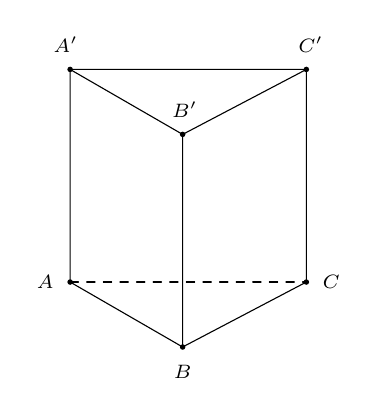
\begin{tikzpicture}[scale=1, font=\footnotesize, line join=round, line cap=round, >=stealth, declare function={a=3; b=0.55*a; h=0.9*a;}]
			\path (0:0) coordinate (A)
			(-30:b) coordinate (B)
			(a,0) coordinate (C)
			\foreach \x in {A,B,C}{(\x)++(90:h) coordinate (\x1)};
			\draw[dashed] (A)--(C);
			\draw (B1)--(A1)--(C1)--cycle
			(A1)--(A)--(B)--(B1)
			(C1)--(C)--(B);
			\foreach \x/\goc/\t in {A/180/A,B/-90/B,C/0/C,A1/100/A',B1/85/B',C1/80/C'}
			\fill (\x) circle (1pt) node[shift={(\goc:9pt)},font=\scriptsize]{$\t$};
		\end{tikzpicture}
	}
	\loigiai{
		Mặt bên là hình vuông có diện tích $16$ nên cạnh hình vuông bằng $4$.\\ Do đó chiều cao lăng trụ bằng $4$ và cạnh đáy tam giác đều bằng $4$.\\
		Diện tích đáy $ABC$ bằng $S_{ABC}=\dfrac{4^2\sqrt{3}}{4}=4\sqrt{3}$.\\
		Thể tích lăng trụ bằng $V=S_{ABC}\cdot h=4\sqrt{3}\cdot4=16\sqrt{3}$.
	}
\end{ex}
%%%=============================%%%

%%%=============EX_4=============%%%
\begin{ex}%[1D2H2-2]%[TDMZZ01]%[Nguyễn Tấn Linh]
	Cho cấp số cộng $(u_n)$ có tổng hai số hạng đầu bằng $3$ và tổng ba số hạng đầu bằng $6$. Công sai của $(u_n)$ bằng
	\choice
	{$3$}
	{$2$}
	{\True $1$}
	{$4$}
	\loigiai{
		Theo giả thiết, ta có hệ phương trình
		\[\heva{& S_2=3 \\ & S_3=6} \Leftrightarrow \heva{& 2u_1+d=3 \\ & 3u_1+3d=6} \Leftrightarrow \heva{& 2u_1+d=3 \\ & u_1+d=2} \Leftrightarrow \heva{& u_1=1 \\ & d=1.}\]
		Vậy công sai của cấp số cộng bằng $1$.
	}
\end{ex}
%%%=============================%%%

%%%=============EX_5=============%%%
\begin{ex}%[2D3N1-2]%[TDMZZ01]%[Phạm Hải Dương]
	Cho mẫu số liệu ghép nhóm $M$ với bảng tần số ghép nhóm như sau:
	\begin{center}
		\begin{tabular}{|c|c|c|c|c|c|c|}
			\hline
			Nhóm & $[8;10)$ & $[10;12)$ & $[12;14)$ & $[14;16)$ & $[16;18)$ & $[18;19)$ \\ \hline
			Tần số & $6$ & $6$ & $8$ & $4$ & $6$ & $7$ \\ \hline
		\end{tabular}
	\end{center}
	Hãy xác định khoảng biến thiên của mẫu số liệu $M$.
	\choice
	{$12$}
	{\True $11$}
	{$19$}
	{$8$}
	\loigiai{
		Khoảng biến thiên của mẫu số liệu $M$ là $R=19-8=11$.
	}
\end{ex}
%%%=============================%%%

%%%=============EX_6=============%%%
\begin{ex}%[2D1N4-1]%[TDMZZ01]%[Nguyễn Sơn Thành]
	Số đường tiệm cận của đồ thị hàm số $y = \dfrac{2x - 1}{3x + 1}$ là
	\choice
	{\True $2$}
	{$1$}
	{$0$}
	{$3$}
	\loigiai{
		Ta có
		\begin{itemize}
			\item Tập xác định là $\mathscr{D}=\mathbb{R}\setminus\left\{-\dfrac{1}{3}\right\}$.
			\item $\displaystyle\lim\limits_{x\to+\infty}\dfrac{2x - 1}{3x + 1}=\dfrac{2}{3}$, $\displaystyle\lim\limits_{x\to-\infty}\dfrac{2x - 1}{3x + 1}=\dfrac{2}{3}$ suy ra $y=\dfrac{2}{3}$ là tiệm cận ngang của đồ thị hàm số.
			\item $\displaystyle\lim\limits_{x \to \left(-\frac{1}{3}\right)^+} \dfrac{2x - 1}{3x + 1}=-\infty$, $\displaystyle\lim\limits_{x \to \left(-\frac{1}{3}\right)^-} \dfrac{2x - 1}{3x + 1}=+\infty$ suy ra $x=-\dfrac{1}{3}$ là tiệm cận đứng của đồ thị hàm số.
		\end{itemize}
		Vậy đồ thị hàm số có $2$ đường tiệm cận.
	}
\end{ex}
%%%=============================%%%

%%%=============EX_7=============%%%
\begin{ex}%[2D4N1-3]%[TDMZZ01]%[Bồ Văn Hậu]
	Họ nguyên hàm của hàm số $f(x)=\cos x$ là
	\choice
	{$-\sin x + C$}
	{$-\cos x + C$}
	{$\cos x + C$}
	{\True $\sin x + C$}
	\loigiai{
		Với mọi $x\in \mathbb{R}$ thì $\left(\sin x\right)'=\cos x$ nên \[\displaystyle\int \cos x \mathrm{\,d}x=\sin x +C.\]
	}
\end{ex}
%%%=============================%%%

%%%=============EX_8=============%%%
\begin{ex}%[2D4N3-1]%[TDMZZ01]%[Lê Phúc]
	Cho hình phẳng $(H)$ giới hạn bởi các đường thẳng $y=f(x)$, $Ox$, $x=a$, $x=b$ ($a>b$). Diện tích hình phẳng $(H)$ được tính theo công thức là
	\choice
	{$S=\displaystyle\int\limits^b_a f(x) \mathrm{\,d}x$}
	{$S=\pi\displaystyle\int\limits^a_b \left|f(x)\right| \mathrm{\,d}x$}
	{\True $S=\displaystyle\int\limits^a_b \left|f(x)\right| \mathrm{\,d}x$}
	{$S=\pi\displaystyle\int\limits^1_0 \left[f(x)\right]^2 \mathrm{\,d}x$}
	\loigiai{
		Diện tích hình phẳng $(H)$ là $S=\displaystyle\int\limits^a_b \left|f(x)\right| \mathrm{\,d}x$.
	}
\end{ex}
%%%=============================%%%

%%%=============EX_9=============%%%
\begin{ex}%[2D1N5-3]%[TDMZZ01]%[Trần Văn Thiện]
	\immini[thm]{Cho đồ thị hàm số $y=f(x)$ như hình vẽ bên. Hỏi hàm số $f(x)$ có thể là hàm số nào dưới đây?
		\choice
		{$f(x)=ax^4+bx^2+c$}
		{$f(x)=ax^2+bx+c$}
		{\True $f(x)=ax^3+bx^2+cx+d$}
		{$f(x)=\dfrac{ax+b}{cx+d}$}
	}
	{ 	
		\begin{tikzpicture}[scale=1, font=\footnotesize, line join=round, line cap=round, >=stealth]
			\draw[->] (-1.5,0)--(3.2,0) node[shift={(-100:7pt)},font=\footnotesize]{$x$};
			\draw[->] (0,-1)--(0,2) node[shift={(180:7pt)},font=\footnotesize]{$y$};
			\fill (0,0) circle (1pt) node[shift={(225:9pt)},font=\footnotesize]{$O$};
			\tikzset{declare function={f (\x)=1/2*(\x)^3-3/2*(\x)^2+3/2;}}
			\begin{scope}
				\draw[samples=100,smooth] plot[domain=-1.05:3] (\x,{f (\x)});
			\end{scope}
			\node[left] at (2.9,1.1) {$f (x)$};
		\end{tikzpicture}
	}
	\loigiai{
		Từ đồ thị hàm số đã cho ta nhận thấy đây là đồ thị hàm số đa thức bậc $3$.
	}
\end{ex}
%%%=============================%%%

%%%=============EX_10=============%%%
\begin{ex}%[2H2N2-4]%[TDMZZ01]%[Đình Nguyên]
	Trong không gian $Oxyz$, khoảng cách từ điểm $M(2;1;-3)$ đến gốc tọa độ $O$ bằng
	\choice
	{\True $\sqrt{14}$}
	{$\sqrt{5}$}
	{$\sqrt{10}$}
	{$0$}
	\loigiai{
		Khoảng cách từ điểm $M(2;1;-3)$ đến gốc tọa độ $O(0;0;0)$ là
		\[OM = \sqrt{2^2 + 1^2 + (-3)^2} = \sqrt{14}.\]
	}
\end{ex}
%%%=============================%%%

%%%=============EX_11=============%%%
\begin{ex}%[2H5H3-2]%[TDMZZ01]%[Huỳnh Quốc Đạt]
	Trong không gian $Oxyz$, cho một mặt cầu $(S)$ có phương trình: $x^2+y^2+z^2-2z-1=0$. Diện tích mặt cầu $(S)$ bằng
	\choice
	{\True $8\pi$}
	{$16\pi$}
	{$4\pi$}
	{$8\dfrac{\pi}{3}$}
	\loigiai{
		Ta có $x^2+y^2+z^2-2z-1=0\Rightarrow \heva{&a=0\\&b=0\\&c=1\\&d=-1}\Rightarrow R=\sqrt{a^2+b^2+c^2-d}=\sqrt{0^2+0^2+1^2+1}=\sqrt{2}$.\\
		Diện tích mặt cầu $(S)$ bằng $S=4\pi\cdot \left(\sqrt{2}\right)^2=8\pi$.
	}
\end{ex}
%%%=============================%%%

%%%=============EX_12=============%%%
\begin{ex}%[2H2H1-2]%[TDMZZ01]%[Nguyễn Trí Minh Tuấn]
	\immini[thm]{Cho hình hộp chữ nhật $ABCD. A'B'C'D'$. Đáp án nhận xét \textbf{đúng} là
		\choice
		{$\left|\overrightarrow{AC}+\overrightarrow{CC'}\right|
			=\left|\overrightarrow{AD}+\overrightarrow{DB'}\right|$}
		{$\left|\overrightarrow{BD}+\overrightarrow{DA'}\right|
			=\left|\overrightarrow{BD'}+\overrightarrow{D'A}\right|$}
		{$\left|\overrightarrow{DB}+\overrightarrow{BB'}\right|
			=\left|\overrightarrow{DC'}+\overrightarrow{C'B}\right|$}
		{\True $\left|\overrightarrow{AB}+\overrightarrow{BC'}\right|
			=\left|\overrightarrow{CD}+\overrightarrow{D'A}\right|$}
	}{
		\begin{tikzpicture}[scale=1, font=\footnotesize, line join=round, line cap=round, >=stealth, declare function={a=3; b=0.45*a; h=0.65*a;}]
			\path (0:0) coordinate (A)
			(220:b) coordinate (B)
			($(B)+(a,0)$) coordinate (C)
			(a,0) coordinate (D)
			\foreach \x in {A,B,C,D}{(\x)++(90:h) coordinate (\x1)};
			\draw[dashed] (A1)--(A)--(B) (A)--(D);
			\draw (B1)--(A1)--(D1)--(C1) (D1)--(D)--(C) (B)--(C)--(C1)--(B1)--cycle;
			\foreach \x/\goc/\t in {A/45/A,B/-90/B,C/-90/C,D/0/D,A1/90/A',B1/90/B',C1/90/C',D1/90/D'}
			\fill (\x) circle (1pt) node[shift={(\goc:7pt)},font=\scriptsize]{$\t$};
		\end{tikzpicture}
	}
	\loigiai{
		Ta có $\left|\overrightarrow{AB}+\overrightarrow{BC'}\right|
		=\left|\overrightarrow{AC'}\right|$.\\
		Lại có
		$\left|\overrightarrow{CD}+\overrightarrow{D'A}\right|=\left|\overrightarrow{C'D'}+\overrightarrow{D'A}\right|=\left|\overrightarrow{C'A}\right|=\left|\overrightarrow{AC'}\right|$.\\
		Do đó $\left|\overrightarrow{AB}+\overrightarrow{BC'}\right|
		=\left|\overrightarrow{CD}+\overrightarrow{D'A}\right|$.
	}
\end{ex}
%%%=============================%%%
\Closesolutionfile{ans}

\cauds
\Opensolutionfile{ans}[ans/ansTN-DungSai]
%%%=============EX_13=============%%%
\begin{ex}%[2D1V5-1]%[TDMZZ01]%[Văn Minh Thoại]
	\immini[thm]{
		Cho hàm số $y=f(x)$ có đồ thị $(C)$ như hình vẽ bên. Biết rằng các nghiệm bội chỉ được tính là một nghiệm.
		\choiceTF
		{Đồ thị của hàm số $y=\dfrac{1}{f(x)}$ có tất cả $4$ đường tiệm cận đứng và ngang}
		{\True $(C)$ có $4$ điểm cực trị}
		{\True Phương trình $\sqrt{f(x)}\cdot\sqrt{f'(x)}=0$ có tất cả $5$ nghiệm thực}
		{Nếu hàm số $F(x)$ là một nguyên hàm của hàm số $f(x)$ thì đồ thị của hàm số $y=F(x)$ có $4$ điểm cực trị}
	}{
		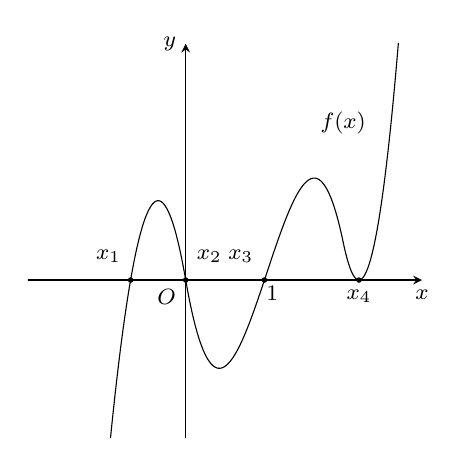
\begin{tikzpicture}[scale=1, font=\footnotesize, line join=round, line cap=round, >=stealth, declare function={yL (\x) = -8.228571*(\x+0.35)^2 + 1.008; yC (\x) = -2.76*(\x)^3 + 8.52*(\x)^2 - 5.76*(\x); yR (\x) = 12*(\x-2.2)^2;}]
			\def \xmin{-2}
			\def \xmax{3}
			\def \ymin{-2}
			\def \ymax{3}
			\draw[->] (\xmin,0)--(\xmax,0) node[below] {$x$};
			\draw[->] (0,\ymin)--(0,\ymax) node[left] {$y$};
			\fill (0,0) circle (1pt) node[below left] {$O$};
			\fill (1,0) circle (1pt) node[shift=(-60:0.2)] {$1$};
			\clip (\xmin,\ymin) rectangle (\xmax,\ymax);
			\draw[smooth, samples=100, domain=\xmin:0] plot (\x,{yL (\x)});
			\draw[smooth, samples=100, domain=0:2.0] plot (\x,{yC (\x)});
			\draw[smooth, samples=100, domain=2.0:\xmax] plot (\x,{yR (\x)});
			\node at (2,2) {$f(x)$};
			\fill (-0.7,0) circle (1pt) node[left, shift={(0,0.3)}] {$x_1$};
			\node at (0.3,0.3) {$x_2$};
			\node at (0.7,0.3) {$x_3$};
			\fill (2.2,0) circle (1pt) node[below] {$x_4$};
		\end{tikzpicture}
	}
	\loigiai{
		Dựa vào đồ thị hàm số $(C)$, ta có
		\begin{itemchoice}
			\itemch 
			Từ đồ thị ta thấy $\lim\limits_{x \to \pm \infty} f(x) = +\infty$ nên $\lim\limits_{x \to \pm \infty} \dfrac{1}{f(x)} = 0$, do đó đồ thị hàm số $y=\dfrac{1}{f(x)}$ có $1$ đường tiệm cận ngang là $y=0$.\\
			Mặt khác, phương trình $f(x)=0$ có $4$ nghiệm phân biệt nên đồ thị hàm số $y=\dfrac{1}{f(x)}$ có $4$ đường tiệm cận đứng.\\
			Vậy đồ thị hàm số $y=\dfrac{1}{f(x)}$ có tất cả $1+4=5$ đường tiệm cận đứng và ngang.
			\itemch 
			Quan sát đồ thị, ta thấy hàm số $y=f(x)$ có $2$ điểm cực đại (lồi) và $2$ điểm cực tiểu (lõm).\\ Do đó $(C)$ có $4$ điểm cực trị.
			\itemch 
			Điều kiện xác định $\heva{&f(x) \ge 0 \\ &f'(x) \ge 0}$ (tức là đồ thị nằm phía trên trục hoành và hàm số đang đồng biến hoặc đạt cực trị).\\
			Ta có $\sqrt{f(x)}\cdot\sqrt{f'(x)}=0 \Leftrightarrow \hoac{&f(x)=0 \\ &f'(x)=0.}$
			\begin{itemize}
				\item Xét $f(x)=0$: Dựa vào đồ thị, phương trình có $4$ nghiệm phân biệt.
				\begin{itemize}
					\item Tại $2$ nghiệm mà đồ thị cắt trục hoành và đi lên, hàm số đồng biến nên $f'(x) > 0$ (thỏa mãn điều kiện). Ta nhận $2$ nghiệm này.
					\item Tại nghiệm mà đồ thị cắt trục hoành và đi xuống (gốc tọa độ $O$), hàm số nghịch biến nên $f'(x) < 0$ (không thỏa mãn điều kiện). Ta loại nghiệm này.
					\item Tại điểm tiếp xúc với trục hoành, hàm số đạt cực tiểu nên $f'(x) = 0$ (thỏa mãn điều kiện). Ta nhận nghiệm này.
				\end{itemize}
				Suy ra phương trình $f(x)=0$ cho ta $3$ nghiệm thỏa mãn điều kiện.
				\item Xét $f'(x)=0$: Phương trình có $4$ nghiệm phân biệt tương ứng là hoành độ của $4$ điểm cực trị.
				\begin{itemize}
					\item Tại $2$ điểm cực đại, đồ thị nằm phía trên trục hoành nên $f(x) > 0$ (thỏa mãn điều kiện). Ta nhận $2$ nghiệm này.
					\item Tại điểm cực tiểu nằm phía dưới trục hoành, ta có $f(x) < 0$ (không thỏa mãn điều kiện). Ta loại nghiệm này.
					\item Tại điểm cực tiểu nằm trên trục hoành, ta có $f(x) = 0$ (thỏa mãn điều kiện, tuy nhiên nghiệm này đã trùng và được đếm ở trường hợp $f(x)=0$).
				\end{itemize}
				Suy ra phương trình $f'(x)=0$ cho ta thêm $2$ nghiệm mới thỏa mãn điều kiện.
			\end{itemize}
			Vậy phương trình đã cho có tất cả $3+2=5$ nghiệm thực phân biệt.
			\itemch 
			Vì $F(x)$ là nguyên hàm của $f(x)$ nên $F'(x) = f(x)$.\\
			Số điểm cực trị của hàm số $y=F(x)$ bằng số lần $F'(x)$ (tức là $f(x)$) đổi dấu.\\
			Dựa vào đồ thị, ta thấy $f(x)$ cắt ngang qua trục hoành tại $3$ điểm phân biệt nên $f(x)$ đổi dấu $3$ lần.\\
			Vậy đồ thị hàm số $y=F(x)$ chỉ có $3$ điểm cực trị.
		\end{itemchoice}
	}
\end{ex}
%%%=============================%%%

%%%=============EX_14=============%%%
\begin{ex}%[2D4V2-6]%[TDMZZ01]%[Dương Công Tạo]
	\immini[thm]{Một đoàn tàu dài $140$\,m đang chuyển động thẳng đều trên một đường ray với tốc độ $25$\,m/s thì thấy ở phía trước $450$\,m so với đầu tàu $A$ có đầu $C$ của một chiếc cầu dài $270$\,m. Người lái tàu ngay sau đó $5$\,giây bắt đầu cho tàu giảm tốc độ theo gia tốc $a=-bt$\,(m/s$^2$), với $t$ tính theo giây và là thời gian tính từ lúc bắt đầu giảm tốc, $b$ là số thực dương. Biết rằng sau khi giảm tốc được $12$\,giây thì đầu tàu đến điểm $D$ và đạt tốc độ $10$\,m/s. Tại $D$ bắt đầu cho tàu chuyển động đều để đi qua cầu cho an toàn.}{
	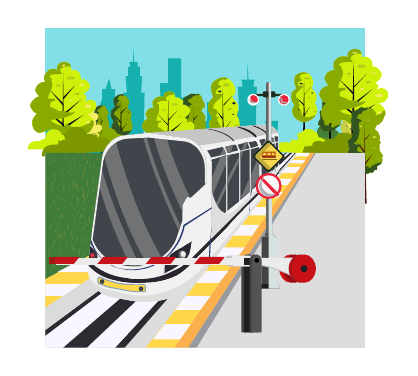
\begin{tikzpicture}[scale=0.15,line cap=round,line join=round,semithick,yscale=-1]
		\definecolor{c82dfe7}{RGB}{130,223,231}
		\definecolor{c16b0ae}{RGB}{22,176,174}
		\definecolor{c438138}{RGB}{67,129,56}
		\definecolor{c89a900}{RGB}{137,169,0}
		\definecolor{c040305}{RGB}{4,3,5}
		\definecolor{c9bad23}{RGB}{155,173,35}
		\definecolor{c325421}{RGB}{50,84,33}
		\definecolor{cf6ee64}{RGB}{246,238,100}
		\definecolor{c07060a}{RGB}{7,6,10}
		\definecolor{c2e283d}{RGB}{46,40,61}
		\definecolor{ccff009}{RGB}{207,240,9}
		\definecolor{c89ab00}{RGB}{137,171,0}
		\definecolor{c7d9700}{RGB}{125,151,0}
		\definecolor{c110f19}{RGB}{17,15,25}
		\definecolor{cf4ed63}{RGB}{244,237,99}
		\definecolor{c4b1910}{RGB}{75,25,16}
		\definecolor{cf6ef63}{RGB}{246,239,99}
		\definecolor{c050407}{RGB}{5,4,7}
		\definecolor{cdddddd}{RGB}{221,221,221}
		\definecolor{c407d3a}{RGB}{64,125,58}
		\definecolor{c969a41}{RGB}{150,154,65}
		\definecolor{cfab04d}{RGB}{250,176,77}
		\definecolor{c2b2c31}{RGB}{43,44,49}
		\definecolor{cf9f6ff}{RGB}{249,246,255}
		\definecolor{cffd749}{RGB}{255,215,73}
		\definecolor{cdbdbdb}{RGB}{219,219,219}
		\definecolor{cf1f1f1}{RGB}{241,241,241}
		\definecolor{c40454b}{RGB}{64,69,75}
		\definecolor{cc6c6c6}{RGB}{198,198,198}
		\definecolor{c2b252f}{RGB}{43,37,47}
		\definecolor{c2c3d73}{RGB}{44,61,115}
		\definecolor{cdedede}{RGB}{222,222,222}
		\definecolor{c231f20}{RGB}{35,31,32}
		\definecolor{c717274}{RGB}{113,114,116}
		\definecolor{c87a2b4}{RGB}{135,162,180}
		\definecolor{c2a2634}{RGB}{42,38,52}
		\definecolor{c3e4245}{RGB}{62,66,69}
		\definecolor{cf2f2f2}{RGB}{242,242,242}
		\definecolor{c24272c}{RGB}{36,39,44}
		\definecolor{c929397}{RGB}{146,147,151}
		\definecolor{cf12b4c}{RGB}{241,43,76}
		\definecolor{c7c353d}{RGB}{124,53,61}
		\definecolor{c979a9f}{RGB}{151,154,159}
		\definecolor{c666666}{RGB}{102,102,102}
		\definecolor{c1f2b1f}{RGB}{31,43,31}
		\definecolor{c444444}{RGB}{68,68,68}
		\definecolor{c545454}{RGB}{84,84,84}
		\definecolor{c1f1f1f}{RGB}{31,31,31}
		\definecolor{cd6e2e2}{RGB}{214,226,226}
		\definecolor{cea243b}{RGB}{234,36,59}
		\definecolor{cfcf8f7}{RGB}{252,248,247}
		\definecolor{cf6d852}{RGB}{246,216,82}
		\definecolor{cc05706}{RGB}{192,87,6}
		\definecolor{c7f1f23}{RGB}{127,31,35}
		\definecolor{c856b0e}{RGB}{133,107,14}
		\definecolor{cb09a34}{RGB}{176,154,52}
		\definecolor{cb0afb7}{RGB}{176,175,183}
		\definecolor{cc5c5c5}{RGB}{197,197,197}
		\definecolor{cebebeb}{RGB}{235,235,235}
		\definecolor{c9f1a13}{RGB}{159,26,19}
		\definecolor{cc7131c}{RGB}{199,19,28}
		\definecolor{cececec}{RGB}{236,236,236}
		\definecolor{c1e1e1e}{RGB}{30,30,30}
		\definecolor{cca1117}{RGB}{202,17,23}
		\definecolor{c950e12}{RGB}{149,14,18}
		\definecolor{cc3c3c3}{RGB}{195,195,195}
		\definecolor{caf1418}{RGB}{175,20,24}
		\path[fill=white,opacity=0] (0,0) rectangle (27.1,27.1);
		\path[fill=c82dfe7] (0,0) rectangle (27.1,27.1);
		\path[fill=c16b0ae] (0.1,10.6) -- (19.8,10.6) -- (19.8,9.5) -- (19.6,9.5) -- (19.7,7.9) -- (18.6,7.9) -- (18.7,8.7) -- (17.8,8.7) -- (17.9,5) -- (17.6,5) -- (17.7,4.4) -- (17.2,4.4) -- (17.1,3) -- (17.1,3) -- (17.1,4.4) -- (16.6,4.4) -- (16.7,5) -- (16.3,5) -- (16.4,7) -- (15.3,7) -- (15.4,9.5) -- (15,9.5) -- (15.1,6.3) -- (14.4,6.3) -- (14.4,5.6) -- (14.3,5.6) -- (14.3,6.3) -- (13.7,6.3) -- (13.7,7.9) -- (13,7.9) -- (13,9.9) -- (12.6,9.9) -- (12.8,6.1) -- (12.1,6.1) -- (12.1,5.9) -- (11.5,5.9) -- (11.5,2.6) -- (10.4,2.6) -- (10.4,4.7) -- (9.7,4.7) -- (9.8,7.6) -- (9.6,7.6) -- (9.5,6.8) -- (9.5,6.8) -- (9.4,7.6) -- (8.7,7.6) -- (8.8,9.8) -- (8.3,9.8) -- (8.4,5.5) -- (8.1,5.5) -- (8.2,4.1) -- (8,4.1) -- (8,3.3) -- (7.8,3.3) -- (7.8,2.9) -- (7.5,2.9) -- (7.5,1.6) -- (7.5,1.6) -- (7.4,2.9) -- (7.1,2.9) -- (7.2,3.3) -- (7,3.3) -- (7,4.1) -- (6.8,4.1) -- (6.9,5.5) -- (6.6,5.5) -- (6.6,7.3) -- (6,7.3) -- (6,6.6) -- (5.9,6) -- (5.9,5.2) -- (5.6,5.2) -- (5.4,4.3) -- (5.1,5.2) -- (4.8,5.2) -- (4.8,6) -- (4.6,6.6) -- (4.7,9.4) -- (4.3,9.4) -- (4.4,7.6) -- (4.1,7.6) -- (4.2,7.2) -- (2.9,7.2) -- (2.9,7.6) -- (2.7,7.6) -- (2.7,8.4) -- (2.4,8.4) -- (2.5,5.3) -- (0.8,5.3) -- (0.9,7.2) -- (0,7.2) -- (0.1,10.6)-- cycle;
		\path[fill=c438138] (25.7,9.3).. controls +(0:0) and +(0:0).. (25.6,9.3).. controls +(-90:0.2) and +(0:0.2).. (25.2,8.9).. controls +(180:0.1) and +(-45:0.1).. (24.9,9).. controls +(-115:0.2) and +(0:0.2).. (24.4,8.6).. controls +(0:0) and +(0:0).. (24.3,8.6).. controls +(-115:0.2) and +(0:0.3).. (23.7,8.2).. controls +(180:0.4) and +(-90:0.3).. (23,8.8).. controls +(0:0) and +(0:0).. (23,8.9).. controls +(0:0) and +(0:0).. (23,8.9).. controls +(180:0.2) and +(-65:0.2).. (22.5,9.2).. controls +(-90:0.1) and +(0:0.1).. (22.3,9.1).. controls +(180:0.4) and +(-90:0.3).. (21.6,9.7) -- (22.7,9.7) -- (22.8,9.7) -- (23,9.7) -- (23.1,9.7) -- (25,9.7) -- (25.2,9.7) -- (25.3,9.7) -- (25.6,9.7) -- (26.1,9.7).. controls +(0:0) and +(0:0).. (26.1,9.7).. controls +(-90:0.2) and +(0:0.2).. (25.7,9.3) -- cycle;
		\path[fill=c89a900] (24.9,7.4).. controls +(-135:0.1) and +(0:0).. (24.8,7.3).. controls +(0:0) and +(0:0).. (24.9,7.2).. controls +(-90:0.1) and +(0:0).. (24.8,7.1).. controls +(-65:0.2) and +(45:0.1).. (24.8,6.7).. controls +(-90:0.1) and +(90:0.1).. (24.6,6.5).. controls +(0:0) and +(90:0.1).. (24.7,6.2).. controls +(0:0.1) and +(-90:0.1).. (24.8,6.3).. controls +(-45:0.1) and +(45:0.1).. (24.7,5.8).. controls +(-90:0.2) and +(25:0.2).. (24.4,5.4).. controls +(180:0.1) and +(0:0.1).. (24.1,5.4) -- (24,5.4).. controls +(180:0.1) and +(0:0).. (23.9,5.4).. controls +(0:0) and +(0:0).. (23.9,5.4).. controls +(180:0.1) and +(0:0.1).. (23.7,5.5).. controls +(0:0) and +(0:0.1).. (23.6,5.5).. controls +(135:0.1) and +(180:0.2).. (23.5,5.8).. controls +(115:0.2) and +(-135:0.1).. (23.5,6.3).. controls +(135:0.1) and +(-90:0.1).. (23.4,6.5).. controls +(0:0) and +(0:0).. (23.5,6.5).. controls +(135:0.1) and +(-90:0.2).. (23.4,7).. controls +(180:0.1) and +(-90:0.1).. (23.2,7.2).. controls +(0:0) and +(0:0).. (23.3,7.2).. controls +(135:0.1) and +(180:0.1).. (23.3,7.4).. controls +(90:0.1) and +(180:0.1).. (23.3,7.7).. controls +(135:0.1) and +(-90:0.1).. (23.1,8.1).. controls +(90:0.1) and +(155:0.2).. (23.3,8.3).. controls +(90:0.1) and +(-135:0.1).. (23.3,8.6).. controls +(-90:0.1) and +(0:0).. (23.4,8.5).. controls +(90:0.1) and +(180:0.1).. (23.6,8.8).. controls +(0:0.1) and +(180:0.1).. (23.8,8.7).. controls +(0:0) and +(0:0).. (23.9,8.8).. controls +(0:0.2) and +(135:0.1).. (24.4,8.7).. controls +(45:0.1) and +(135:0.1).. (24.6,8.5).. controls +(45:0.1) and +(45:0.1).. (24.7,8.4).. controls +(0:0.2) and +(45:0.1).. (25,8).. controls +(-25:0.2) and +(115:0.2).. (24.9,7.4) -- cycle;
		\path[fill=c040305] (24,10.3) -- (24.1,6.2) -- (24.2,10.3) -- (24,10.3)-- cycle;
		\path[fill=c040305] (24.5,7.7) -- (24.1,8.2) -- (24.1,8.3) -- (24.5,7.7)-- cycle;
		\path[fill=c040305] (23.7,7.2).. controls +(0:0) and +(0:0).. (24.1,7.6) -- (24.1,7.7) -- (23.7,7.2) -- cycle;
		\path[fill=c040305] (24.3,6.7) -- (24.1,7) -- (24.1,7) -- (24.3,6.7)-- cycle;
		\path[fill=c9bad23,opacity=0.5] (24.4,6).. controls +(90:0.1) and +(0:0.1).. (24.3,6.1).. controls +(180:0.1) and +(90:0.1).. (24.1,6).. controls +(0:0) and +(180:0.1).. (24.3,6).. controls +(0:0.1) and +(0:0).. (24.4,6) -- cycle;
		\path[fill=c9bad23,opacity=0.5] (24.9,8).. controls +(0:0) and +(0:0.1).. (24.7,8).. controls +(0:0) and +(0:0).. (24.6,8).. controls +(0:0) and +(0:0).. (24.7,7.9).. controls +(0:0.1) and +(0:0).. (24.9,8) -- cycle;
		\path[fill=c9bad23,opacity=0.5] (24.5,7.2).. controls +(0:0) and +(0:0.1).. (24.4,7.2).. controls +(180:0.1) and +(0:0).. (24.3,7.2).. controls +(0:0) and +(180:0.1).. (24.4,7.1).. controls +(0:0.1) and +(0:0).. (24.5,7.2) -- cycle;
		\path[fill=c9bad23,opacity=0.5] (24.5,6.3).. controls +(0:0) and +(0:0).. (24.5,6.3).. controls +(180:0.1) and +(0:0).. (24.4,6.3).. controls +(0:0) and +(180:0.1).. (24.5,6.3).. controls +(0:0) and +(0:0).. (24.5,6.3) -- cycle;
		\path[fill=c9bad23,opacity=0.5];
		\path[fill=c325421] (25,8.2).. controls +(180:0.2) and +(-90:0.1).. (24.4,8.5).. controls +(-135:0.1) and +(0:0).. (24.2,8.4).. controls +(0:0) and +(0:0).. (24.2,8.5).. controls +(-105:0.4) and +(65:0.2).. (23.6,8.2).. controls +(-90:0.1) and +(180:0.2).. (23.7,7.9).. controls +(-90:0.2) and +(90:0.1).. (24,7.6).. controls +(135:0.4) and +(-165:0.4).. (23.9,7.4).. controls +(-115:0.2) and +(25:0.2).. (23.5,7.2).. controls +(-25:0.2) and +(90:0.2).. (23.8,6.6).. controls +(-90:0.2) and +(180:0.3).. (24,6.1).. controls +(-135:0.1) and +(0:0.1).. (23.7,5.9).. controls +(-90:0.1) and +(180:0.1).. (23.9,5.7).. controls +(0:0.1) and +(0:0).. (24,5.6).. controls +(0:0.1) and +(155:0.2).. (24.3,5.4).. controls +(0:0.1) and +(-135:0.1).. (24.5,5.5).. controls +(-90:0.1) and +(0:0).. (24.4,5.4).. controls +(180:0.1) and +(0:0.1).. (24.1,5.4) -- (24,5.4).. controls +(180:0.1) and +(0:0).. (23.9,5.4).. controls +(0:0) and +(0:0).. (23.9,5.4).. controls +(180:0.1) and +(-45:0.1).. (23.7,5.5).. controls +(0:0) and +(0:0.1).. (23.6,5.5).. controls +(135:0.1) and +(180:0.2).. (23.5,5.8).. controls +(115:0.2) and +(-135:0.1).. (23.5,6.3).. controls +(135:0.1) and +(-90:0.1).. (23.4,6.5).. controls +(0:0) and +(0:0).. (23.5,6.5).. controls +(135:0.1) and +(-90:0.2).. (23.4,7).. controls +(180:0.1) and +(-90:0.1).. (23.2,7.2).. controls +(0:0) and +(0:0).. (23.3,7.2).. controls +(135:0.1) and +(180:0.1).. (23.3,7.4).. controls +(90:0.1) and +(180:0.1).. (23.3,7.7).. controls +(135:0.1) and +(-90:0.1).. (23.1,8.1).. controls +(90:0.1) and +(155:0.2).. (23.3,8.3).. controls +(90:0.1) and +(-135:0.1).. (23.3,8.6).. controls +(-90:0.1) and +(0:0).. (23.4,8.5).. controls +(90:0.1) and +(180:0.1).. (23.6,8.8).. controls +(0:0.1) and +(180:0.1).. (23.8,8.7).. controls +(0:0) and +(0:0).. (23.9,8.8).. controls +(0:0.2) and +(135:0.1).. (24.4,8.7).. controls +(45:0.1) and +(135:0.1).. (24.6,8.5).. controls +(45:0.1) and +(45:0.1).. (24.7,8.4).. controls +(0:0.1) and +(135:0.1).. (25,8.2) -- cycle;
		\path[fill=cf6ee64] (25.3,6.5).. controls +(0:0) and +(160:0.6).. (25.5,5.4).. controls +(0:0) and +(-135:0.6).. (26.4,5.4).. controls +(0:0) and +(-65:0.7).. (26.7,6.4).. controls +(0:0) and +(-135:0.1).. (26.6,6.6).. controls +(45:0.1) and +(0:0).. (26.7,6.7).. controls +(35:0.4) and +(-60:0.6).. (26.8,7.8).. controls +(0:0) and +(-45:0.7).. (26.8,8.9).. controls +(0:0) and +(0:0.7).. (26,9.3).. controls +(0:0) and +(90:0.8).. (25,8.4).. controls +(0:0) and +(135:0.3).. (25.2,8).. controls +(0:0) and +(45:0.1).. (25.1,7.8).. controls +(0:0) and +(150:0.9).. (25.3,6.6).. controls +(0:0) and +(0:0).. (25.3,6.5) -- cycle;
		\path[fill=c07060a] (25.9,11.8) -- (25.9,5.9) -- (26.1,11.8) -- (25.9,11.8)-- cycle;
		\path[fill=c07060a] (26.5,8.1) -- (26,8.8) -- (26,8.9) -- (26.5,8.1)-- cycle;
		\path[fill=c07060a] (25.4,7.4).. controls +(0:0.1) and +(0:0).. (25.9,7.9) -- (25.9,8) -- (25.4,7.4) -- cycle;
		\path[fill=c07060a] (26.5,6.5) -- (26,7.1) -- (26,7.1) -- (26.5,6.5)-- cycle;
		\begin{scope}[opacity=0.5,transparency group]
			\path[fill=c9bad23] (26.8,8.9).. controls +(0:0.1) and +(0:0).. (26.9,8.8).. controls +(180:0.2) and +(0:0.2).. (26.3,9).. controls +(180:0.2) and +(0:0.1).. (25.8,8.8).. controls +(-65:0.4) and +(160:0.5).. (25.7,7.9).. controls +(180:0.1) and +(0:0).. (25.5,7.9).. controls +(-70:0.3) and +(25:0.2).. (25.3,7.3).. controls +(0:0) and +(0:0.1).. (25.2,7.3).. controls +(-105:0.4) and +(125:0.4).. (26,6.3).. controls +(155:0.2) and +(45:0.1).. (25.5,6.3).. controls +(-115:0.2) and +(180:0.2).. (25.8,5.9).. controls +(-90:0.1) and +(45:0.1).. (25.6,5.6).. controls +(-70:0.3) and +(180:0.3).. (26.3,5.3).. controls +(-145:0.4) and +(0:0).. (25.5,5.4).. controls +(160:0.6) and +(0:0).. (25.3,6.5).. controls +(0:0) and +(0:0).. (25.3,6.6).. controls +(150:0.9) and +(0:0).. (25.1,7.8).. controls +(45:0.1) and +(0:0).. (25.2,8).. controls +(135:0.3) and +(0:0).. (25,8.4).. controls +(90:0.8) and +(0:0).. (26,9.3).. controls +(0:0.7) and +(0:0).. (26.8,8.9) -- cycle;
		\end{scope}
		\path[fill=c9bad23,opacity=0.5] (26.4,5.7).. controls +(90:0.1) and +(0:0.1).. (26.2,5.8).. controls +(180:0.2) and +(90:0.1).. (25.9,5.7).. controls +(-90:0.1) and +(180:0.2).. (26.2,5.6).. controls +(0:0.1) and +(-90:0.1).. (26.4,5.7) -- cycle;
		\path[fill=c9bad23,opacity=0.5] (27,8.5).. controls +(0:0) and +(0:0.1).. (26.9,8.6).. controls +(180:0.1) and +(0:0).. (26.7,8.5).. controls +(-90:0.1) and +(180:0.1).. (26.9,8.4).. controls +(0:0.1) and +(-90:0.1).. (27,8.5) -- cycle;
		\path[fill=c9bad23,opacity=0.5] (26.5,7.3).. controls +(90:0.1) and +(0:0.1).. (26.4,7.4).. controls +(180:0.1) and +(90:0.1).. (26.2,7.3).. controls +(0:0) and +(180:0.1).. (26.4,7.3).. controls +(0:0.1) and +(0:0).. (26.5,7.3) -- cycle;
		\path[fill=c9bad23,opacity=0.5] (26.5,6.1).. controls +(0:0) and +(0:0).. (26.5,6.1).. controls +(180:0.1) and +(0:0).. (26.4,6.1).. controls +(0:0) and +(180:0.1).. (26.5,6.1).. controls +(-90:0.1) and +(0:0).. (26.5,6.1) -- cycle;
		\path[fill=c9bad23,opacity=0.5] (26.2,8.2).. controls +(0:0) and +(0:0.1).. (26.1,8.2).. controls +(0:0) and +(0:0).. (26,8.2).. controls +(-90:0.1) and +(0:0).. (26.1,8.1).. controls +(0:0.1) and +(-90:0.1).. (26.2,8.2) -- cycle;
		\path[fill=c2e283d] (26.8,6.9).. controls +(90:0.1) and +(0:0.1).. (26.7,7).. controls +(180:0.1) and +(90:0.1).. (26.5,6.9).. controls +(0:0) and +(0:0).. (26.6,6.9).. controls +(0:0.1) and +(0:0).. (26.8,6.9) -- cycle;
		\path[fill=c2e283d] (25.8,6.2).. controls +(0:0) and +(0:0.1).. (25.7,6.2).. controls +(180:0.1) and +(0:0).. (25.6,6.2).. controls +(-90:0.1) and +(180:0.1).. (25.7,6.1).. controls +(0:0.1) and +(-90:0.1).. (25.8,6.2) -- cycle;
		\path[fill=c2e283d] (26.2,5.3).. controls +(0:0) and +(0:0).. (26.1,5.4).. controls +(0:0) and +(0:0).. (26,5.3).. controls +(0:0) and +(0:0).. (26.1,5.3).. controls +(0:0) and +(0:0).. (26.2,5.3) -- cycle;
		\path[fill=c2e283d] (26.7,7.7).. controls +(0:0) and +(0:0.1).. (26.6,7.7).. controls +(0:0) and +(0:0).. (26.6,7.7).. controls +(0:0) and +(0:0).. (26.6,7.7).. controls +(0:0.1) and +(0:0).. (26.7,7.7) -- cycle;
		\path[fill=c2e283d] (25.6,8.3).. controls +(0:0) and +(0:0).. (25.5,8.4).. controls +(0:0) and +(0:0).. (25.5,8.3).. controls +(0:0) and +(0:0).. (25.5,8.3).. controls +(0:0) and +(0:0).. (25.6,8.3) -- cycle;
		\path[fill=ccff009] (21.2,5).. controls +(0:0) and +(155:0.7).. (21.4,3.9).. controls +(0:0) and +(-135:0.4).. (22.3,3.9).. controls +(0:0) and +(-65:0.7).. (22.6,5).. controls +(0:0) and +(-155:0.2).. (22.6,5.2).. controls +(90:0.1) and +(180:0.1).. (22.7,5.3).. controls +(45:0.3) and +(-60:0.6).. (22.8,6.4).. controls +(0:0) and +(-45:0.7).. (22.8,7.5).. controls +(0:0) and +(-10:0.7).. (21.9,8).. controls +(0:0) and +(90:0.9).. (20.9,7).. controls +(0:0) and +(135:0.3).. (21.1,6.6).. controls +(0:0) and +(45:0.1).. (21,6.4).. controls +(0:0) and +(150:0.9).. (21.2,5.2).. controls +(0:0) and +(45:0.1).. (21.2,5) -- cycle;
		\path[fill=c07060a] (21.8,10.4) -- (21.9,4.5) -- (22,10.4) -- (21.8,10.4)-- cycle;
		\path[fill=c07060a] (22.4,6.7) -- (21.9,7.4) -- (21.9,7.5) -- (22.4,6.7)-- cycle;
		\path[fill=c07060a] (21.3,6).. controls +(0:0.1) and +(0:0).. (21.9,6.5) -- (21.9,6.6) -- (21.3,6) -- cycle;
		\path[fill=c07060a] (22.5,5) -- (21.9,5.7) -- (21.9,5.7) -- (22.5,5)-- cycle;
		\path[fill=c89ab00] (22.8,7.5).. controls +(0:0) and +(0:0).. (22.9,7.4).. controls +(180:0.2) and +(0:0.2).. (22.2,7.6).. controls +(180:0.2) and +(25:0.2).. (21.7,7.4).. controls +(-65:0.4) and +(160:0.5).. (21.6,6.5).. controls +(0:0) and +(0:0.1).. (21.4,6.5).. controls +(-65:0.4) and +(20:0.3).. (21.2,5.9).. controls +(0:0) and +(0:0).. (21.2,5.9).. controls +(-115:0.4) and +(125:0.4).. (21.9,4.9).. controls +(155:0.2) and +(0:0.2).. (21.4,4.9).. controls +(-110:0.3) and +(180:0.2).. (21.7,4.5).. controls +(-90:0.1) and +(25:0.2).. (21.5,4.2).. controls +(-75:0.4) and +(180:0.3).. (22.3,3.9).. controls +(-145:0.5) and +(0:0).. (21.4,3.9).. controls +(155:0.7) and +(0:0).. (21.2,5).. controls +(45:0.1) and +(0:0).. (21.2,5.2).. controls +(150:0.9) and +(0:0).. (21,6.4).. controls +(45:0.1) and +(0:0).. (21.1,6.6).. controls +(135:0.3) and +(0:0).. (20.9,7).. controls +(90:0.9) and +(0:0).. (21.9,8).. controls +(-10:0.7) and +(0:0).. (22.8,7.5) -- cycle;
		\path[fill=c9bad23,opacity=0.5] (22.4,4.3).. controls +(0:0) and +(0:0.2).. (22.1,4.4).. controls +(180:0.1) and +(0:0).. (21.9,4.3).. controls +(-90:0.1) and +(180:0.1).. (22.1,4.2).. controls +(0:0.2) and +(-90:0.1).. (22.4,4.3) -- cycle;
		\path[fill=c9bad23,opacity=0.5] (23,7.1).. controls +(0:0) and +(0:0.1).. (22.8,7.2).. controls +(180:0.1) and +(0:0).. (22.7,7.1).. controls +(0:0) and +(180:0.1).. (22.8,7).. controls +(0:0.1) and +(0:0).. (23,7.1) -- cycle;
		\path[fill=c9bad23,opacity=0.5] (22.5,5.9).. controls +(90:0.1) and +(0:0.1).. (22.3,6).. controls +(180:0.1) and +(90:0.1).. (22.2,5.9).. controls +(0:0) and +(180:0.1).. (22.3,5.9).. controls +(0:0.1) and +(0:0).. (22.5,5.9) -- cycle;
		\path[fill=c9bad23,opacity=0.5] (22.5,4.7).. controls +(0:0) and +(0:0.1).. (22.4,4.7).. controls +(0:0) and +(0:0).. (22.3,4.7).. controls +(-90:0.1) and +(0:0).. (22.4,4.6).. controls +(0:0.1) and +(-90:0.1).. (22.5,4.7) -- cycle;
		\path[fill=c9bad23,opacity=0.5] (22.1,6.8).. controls +(0:0) and +(0:0).. (22.1,6.8).. controls +(180:0.1) and +(0:0).. (22,6.8).. controls +(-90:0.1) and +(180:0.1).. (22.1,6.7).. controls +(0:0) and +(-90:0.1).. (22.1,6.8) -- cycle;
		\path[fill=c2e283d] (22.7,5.5).. controls +(90:0.1) and +(0:0.1).. (22.6,5.6).. controls +(0:0) and +(90:0.1).. (22.5,5.5).. controls +(0:0) and +(180:0.1).. (22.6,5.5).. controls +(0:0) and +(0:0).. (22.7,5.5) -- cycle;
		\path[fill=c2e283d] (21.8,4.7).. controls +(90:0.1) and +(0:0.1).. (21.6,4.8).. controls +(0:0) and +(90:0.1).. (21.5,4.7).. controls +(0:0) and +(0:0).. (21.6,4.7).. controls +(0:0.1) and +(0:0).. (21.8,4.7) -- cycle;
		\path[fill=c2e283d] (22.1,3.9).. controls +(0:0) and +(0:0.1).. (22,3.9).. controls +(0:0) and +(0:0).. (22,3.9).. controls +(0:0) and +(0:0).. (22,3.9).. controls +(0:0.1) and +(0:0).. (22.1,3.9) -- cycle;
		\path[fill=c2e283d] (22.6,6.3).. controls +(0:0) and +(0:0).. (22.6,6.3).. controls +(180:0.1) and +(0:0).. (22.5,6.3).. controls +(0:0) and +(180:0.1).. (22.6,6.3).. controls +(0:0) and +(0:0).. (22.6,6.3) -- cycle;
		\path[fill=c2e283d] (21.5,6.9).. controls +(0:0) and +(0:0.1).. (21.4,7).. controls +(0:0) and +(0:0).. (21.4,6.9).. controls +(0:0) and +(0:0).. (21.4,6.9).. controls +(0:0.1) and +(0:0).. (21.5,6.9) -- cycle;
		\path[fill=ccff009] (25.5,10.6).. controls +(0:0.1) and +(0:0).. (25.6,10.6).. controls +(0:0) and +(0:0).. (25.6,10.6).. controls +(0:0) and +(0:0).. (25.5,10.6).. controls +(0:0) and +(0:0).. (25.5,10.6).. controls +(0:0) and +(0:0).. (25.5,10.6).. controls +(0:0) and +(0:0).. (25.4,10.6).. controls +(0:0) and +(0:0).. (25.4,10.6).. controls +(0:0) and +(0:0).. (25.4,10.6).. controls +(0:0) and +(0:0).. (25.4,10.6).. controls +(0:0) and +(0:0).. (25.4,10.6).. controls +(0:0) and +(0:0).. (25.4,10.6).. controls +(-90:0.1) and +(0:0).. (25.4,10.5).. controls +(0:0) and +(0:0).. (25.4,10.5).. controls +(0:0) and +(0:0).. (25.4,10.5).. controls +(0:0) and +(0:0.1).. (25.3,10.5).. controls +(0:0) and +(0:0).. (25.3,10.5).. controls +(0:0) and +(0:0).. (25.3,10.5).. controls +(0:0) and +(0:0).. (25.3,10.5).. controls +(180:0.1) and +(0:0).. (25.2,10.5).. controls +(0:0) and +(0:0).. (25.2,10.5).. controls +(0:0) and +(0:0).. (25.2,10.5).. controls +(0:0) and +(90:0.1).. (25.1,10.4).. controls +(0:0) and +(0:0).. (25.1,10.4).. controls +(0:0) and +(0:0).. (25.1,10.4).. controls +(0:0) and +(0:0.1).. (25,10.4).. controls +(0:0) and +(0:0).. (25,10.4).. controls +(0:0) and +(0:0).. (25,10.4).. controls +(180:0.1) and +(0:0).. (24.9,10.4).. controls +(0:0) and +(0:0).. (24.9,10.4).. controls +(0:0) and +(0:0).. (24.9,10.4).. controls +(0:0) and +(0:0).. (24.9,10.4).. controls +(0:0) and +(0:0).. (24.9,10.4).. controls +(0:0) and +(0:0).. (24.9,10.3).. controls +(0:0) and +(0:0).. (24.9,10.3).. controls +(0:0) and +(0:0).. (24.9,10.3).. controls +(0:0) and +(0:0).. (24.9,10.3).. controls +(-90:0.1) and +(0:0).. (24.9,10.2).. controls +(0:0) and +(0:0.1).. (24.8,10.2).. controls +(0:0) and +(0:0).. (24.8,10.2).. controls +(0:0) and +(90:0.1).. (24.8,10.1).. controls +(0:0) and +(0:0).. (24.8,10.1).. controls +(0:0) and +(0:0).. (24.8,10.1).. controls +(0:0) and +(0:0).. (24.8,10.1).. controls +(0:0) and +(0:0).. (24.8,10.1).. controls +(-90:0.1) and +(0:0).. (24.8,10).. controls +(180:0.1) and +(0:0).. (24.7,10).. controls +(0:0) and +(0:0).. (24.7,10).. controls +(0:0) and +(0:0).. (24.7,10).. controls +(0:0) and +(90:0.1).. (24.7,9.9).. controls +(0:0) and +(0:0.1).. (24.6,9.9).. controls +(0:0) and +(0:0).. (24.6,9.9).. controls +(0:0) and +(0:0).. (24.6,9.9).. controls +(0:0) and +(0:0).. (24.6,9.9).. controls +(0:0) and +(0:0).. (24.6,9.9).. controls +(180:0.1) and +(0:0).. (24.5,9.9).. controls +(-90:0.1) and +(0:0).. (24.5,9.8).. controls +(0:0) and +(0:0).. (24.5,9.8).. controls +(0:0) and +(0:0).. (24.4,9.8).. controls +(0:0) and +(0:0).. (24.4,9.8).. controls +(0:0) and +(0:0).. (24.4,9.8).. controls +(0:0) and +(0:0).. (24.3,9.8).. controls +(0:0) and +(0:0).. (24.3,9.8).. controls +(0:0) and +(0:0).. (24.2,9.8).. controls +(0:0) and +(0:0).. (24.2,9.8).. controls +(0:0) and +(0:0).. (24.2,9.8).. controls +(0:0) and +(0:0.1).. (24.1,9.8).. controls +(0:0) and +(0:0).. (24.1,9.8).. controls +(0:0) and +(0:0).. (24.1,9.8).. controls +(0:0) and +(0:0).. (24.1,9.8).. controls +(180:0.1) and +(0:0).. (24,9.8).. controls +(0:0) and +(0:0).. (24,9.8).. controls +(0:0) and +(0:0).. (24,9.9).. controls +(0:0) and +(0:0).. (24,9.9).. controls +(0:0) and +(0:0.1).. (23.9,9.9).. controls +(0:0) and +(0:0).. (23.9,9.9).. controls +(0:0) and +(0:0).. (23.9,9.8).. controls +(0:0) and +(0:0).. (23.9,9.8).. controls +(0:0) and +(0:0).. (23.9,9.8).. controls +(0:0) and +(0:0).. (23.9,9.7).. controls +(0:0) and +(0:0).. (23.9,9.7).. controls +(0:0) and +(0:0).. (23.9,9.7).. controls +(0:0) and +(0:0).. (23.9,9.7).. controls +(0:0) and +(0:0).. (23.9,9.7).. controls +(0:0) and +(0:0).. (23.9,9.7).. controls +(0:0) and +(0:0).. (23.9,9.7).. controls +(0:0) and +(0:0).. (23.9,9.6).. controls +(0:0) and +(0:0).. (23.9,9.6).. controls +(0:0) and +(0:0).. (23.9,9.6).. controls +(0:0) and +(180:0.1).. (24,9.6).. controls +(0:0) and +(0:0).. (24,9.6).. controls +(0:0) and +(0:0).. (24,9.6).. controls +(0:0) and +(0:0).. (24,9.6).. controls +(0:0) and +(0:0).. (24,9.6).. controls +(0:0) and +(0:0).. (24,9.6).. controls +(0:0) and +(0:0).. (24,9.6).. controls +(0:0) and +(0:0).. (24,9.6).. controls +(0:0) and +(0:0.1).. (23.9,9.6).. controls +(0:0) and +(0:0).. (23.9,9.6).. controls +(0:0) and +(0:0).. (23.9,9.6).. controls +(0:0) and +(0:0).. (23.9,9.6).. controls +(0:0) and +(0:0).. (23.9,9.6).. controls +(0:0) and +(0:0).. (23.9,9.6).. controls +(0:0) and +(0:0).. (23.9,9.6).. controls +(0:0) and +(0:0.1).. (23.8,9.6).. controls +(0:0) and +(0:0).. (23.8,9.6).. controls +(0:0) and +(0:0).. (23.8,9.6).. controls +(0:0) and +(0:0).. (23.8,9.6).. controls +(-45:0.1) and +(0:0).. (23.9,9.5).. controls +(0:0) and +(0:0).. (23.9,9.5).. controls +(0:0) and +(0:0).. (23.9,9.5).. controls +(0:0) and +(0:0).. (23.9,9.5).. controls +(0:0) and +(0:0).. (23.9,9.5).. controls +(0:0) and +(0:0.1).. (23.8,9.5).. controls +(0:0) and +(0:0).. (23.8,9.5).. controls +(0:0) and +(0:0).. (23.8,9.5).. controls +(0:0) and +(0:0).. (23.8,9.5).. controls +(0:0) and +(0:0).. (23.8,9.5).. controls +(0:0) and +(0:0).. (23.8,9.5).. controls +(0:0) and +(0:0).. (23.8,9.5).. controls +(0:0) and +(0:0).. (23.8,9.5).. controls +(0:0) and +(0:0.1).. (23.7,9.5).. controls +(0:0) and +(0:0).. (23.7,9.5).. controls +(0:0) and +(0:0).. (23.7,9.5).. controls +(0:0) and +(0:0).. (23.7,9.5).. controls +(0:0) and +(0:0).. (23.7,9.5).. controls +(0:0) and +(0:0).. (23.7,9.5).. controls +(180:0.1) and +(0:0).. (23.6,9.5).. controls +(-90:0.1) and +(0:0).. (23.6,9.4).. controls +(0:0) and +(0:0).. (23.6,9.4).. controls +(0:0) and +(0:0).. (23.5,9.4).. controls +(0:0) and +(0:0).. (23.5,9.4).. controls +(0:0) and +(0:0).. (23.5,9.4).. controls +(180:0.1) and +(0:0).. (23.4,9.4).. controls +(0:0) and +(90:0.1).. (23.4,9.3).. controls +(0:0) and +(0:0).. (23.4,9.3).. controls +(180:0.1) and +(0:0).. (23.3,9.3).. controls +(0:0) and +(0:0).. (23.2,9.3).. controls +(0:0) and +(0:0).. (23.2,9.3).. controls +(0:0) and +(0:0).. (23.2,9.3).. controls +(0:0) and +(0:0.1).. (23.1,9.2).. controls +(0:0) and +(0:0).. (23.1,9.2).. controls +(0:0) and +(0:0).. (23.1,9.1).. controls +(0:0) and +(0:0).. (23.1,9.1).. controls +(0:0) and +(0:0.1).. (23,9).. controls +(0:0) and +(0:0).. (23,9).. controls +(0:0) and +(90:0.1).. (23,8.9).. controls +(0:0) and +(0:0).. (23,8.9).. controls +(0:0) and +(90:0.1).. (22.9,8.8).. controls +(0:0) and +(0:0).. (22.9,8.8).. controls +(0:0) and +(0:0.1).. (22.8,8.8).. controls +(0:0) and +(0:0).. (22.8,8.8).. controls +(0:0) and +(0:0.1).. (22.7,8.7).. controls +(0:0) and +(0:0).. (22.7,8.7).. controls +(0:0) and +(0:0).. (22.7,8.7).. controls +(0:0) and +(0:0).. (22.7,8.7).. controls +(180:0.1) and +(0:0.1).. (22.5,8.6).. controls +(0:0) and +(0:0).. (22.5,8.6).. controls +(0:0) and +(0:0).. (22.5,8.6).. controls +(180:0.1) and +(0:0).. (22.4,8.6).. controls +(0:0) and +(0:0).. (22.4,8.6).. controls +(0:0) and +(0:0).. (22.3,8.6).. controls +(0:0) and +(0:0).. (22.3,8.6).. controls +(0:0) and +(0:0).. (22.3,8.6).. controls +(0:0) and +(0:0).. (22.3,8.6).. controls +(180:0.1) and +(0:0).. (22.2,8.6).. controls +(0:0) and +(0:0).. (22.2,8.6).. controls +(0:0) and +(0:0).. (22.2,8.6).. controls +(0:0) and +(0:0).. (22.2,8.6).. controls +(0:0) and +(0:0).. (22.2,8.6).. controls +(180:0.1) and +(0:0).. (22.1,8.6).. controls +(0:0) and +(0:0).. (22.1,8.6).. controls +(0:0) and +(0:0).. (22.1,8.6).. controls +(0:0) and +(0:0).. (22.1,8.6).. controls +(0:0) and +(0:0).. (22.1,8.6).. controls +(0:0) and +(0:0).. (22.1,8.6).. controls +(0:0) and +(0:0).. (22.1,8.6).. controls +(0:0) and +(0:0).. (22.1,8.6).. controls +(0:0) and +(0:0).. (22.1,8.6).. controls +(0:0) and +(0:0).. (22.1,8.6).. controls +(0:0) and +(0:0).. (22.1,8.6).. controls +(0:0) and +(0:0).. (22.1,8.6).. controls +(0:0) and +(0:0).. (22.1,8.6).. controls +(0:0) and +(0:0).. (22.1,8.6).. controls +(0:0) and +(0:0).. (22.1,8.6).. controls +(0:0) and +(0:0).. (22.1,8.6).. controls +(0:0) and +(0:0).. (22,8.6).. controls +(0:0) and +(0:0).. (22,8.6).. controls +(135:0.1) and +(-90:0.1).. (21.8,8.8).. controls +(0:0) and +(0:0).. (21.8,8.8).. controls +(0:0) and +(0:0).. (21.7,8.8).. controls +(0:0) and +(0:0).. (21.7,8.8).. controls +(0:0) and +(0:0).. (21.7,8.8).. controls +(0:0) and +(0:0).. (21.7,8.8).. controls +(0:0) and +(0:0).. (21.7,8.8).. controls +(0:0) and +(0:0).. (21.7,8.8).. controls +(135:0.1) and +(0:0).. (21.6,8.9).. controls +(0:0) and +(0:0).. (21.6,8.9).. controls +(0:0) and +(0:0).. (21.5,9).. controls +(0:0) and +(0:0).. (21.5,9).. controls +(0:0) and +(0:0).. (21.5,9).. controls +(0:0) and +(0:0).. (21.5,9).. controls +(0:0) and +(0:0).. (21.5,9).. controls +(0:0) and +(0:0).. (21.5,9).. controls +(0:0) and +(0:0).. (21.5,9).. controls +(-90:0.1) and +(0:0).. (21.5,8.9).. controls +(0:0) and +(0:0).. (21.5,8.9).. controls +(180:0.1) and +(0:0).. (21.4,8.9).. controls +(0:0) and +(0:0).. (21.4,8.9).. controls +(0:0) and +(0:0).. (21.4,8.9).. controls +(0:0) and +(0:0).. (21.4,8.9).. controls +(0:0) and +(0:0).. (21.4,8.9).. controls +(0:0) and +(0:0).. (21.4,8.9).. controls +(0:0) and +(0:0).. (21.4,8.9).. controls +(0:0) and +(0:0).. (21.4,8.9).. controls +(0:0) and +(-90:0.1).. (21.4,9.1).. controls +(0:0) and +(0:0).. (21.4,9.1).. controls +(0:0) and +(0:0).. (21.4,9.1).. controls +(0:0) and +(0:0).. (21.4,9.1).. controls +(0:0) and +(0:0).. (21.4,9).. controls +(0:0) and +(0:0).. (21.4,9).. controls +(180:0.1) and +(0:0).. (21.3,9).. controls +(0:0) and +(0:0).. (21.3,9).. controls +(0:0) and +(0:0).. (21.3,9).. controls +(0:0) and +(0:0).. (21.3,9).. controls +(0:0) and +(0:0).. (21.3,9).. controls +(0:0) and +(0:0).. (21.3,9).. controls +(0:0) and +(0:0).. (21.3,9).. controls +(0:0) and +(-135:0.1).. (21.4,9.2).. controls +(0:0) and +(0:0).. (21.4,9.2).. controls +(0:0) and +(0:0).. (21.4,9.2).. controls +(0:0) and +(0:0).. (21.4,9.2).. controls +(0:0) and +(0:0).. (21.4,9.3).. controls +(0:0) and +(0:0).. (21.4,9.3).. controls +(0:0) and +(-90:0.1).. (21.4,9.4).. controls +(0:0) and +(0:0).. (21.4,9.4).. controls +(0:0) and +(0:0).. (21.4,9.4).. controls +(90:0.1) and +(0:0).. (21.4,9.5).. controls +(0:0) and +(0:0).. (21.4,9.5).. controls +(0:0) and +(0:0).. (21.3,9.5).. controls +(0:0) and +(0:0).. (21.3,9.5).. controls +(0:0) and +(0:0.1).. (21.2,9.5).. controls +(0:0) and +(0:0).. (21.2,9.5).. controls +(0:0) and +(0:0).. (21.2,9.5).. controls +(0:0) and +(0:0).. (21.2,9.5).. controls +(180:0.1) and +(0:0).. (21.1,9.5).. controls +(0:0) and +(0:0).. (21.1,9.5).. controls +(0:0) and +(0:0).. (21.1,9.5).. controls +(180:0.1) and +(0:0).. (21,9.5).. controls +(0:0) and +(0:0).. (21,9.5).. controls +(0:0) and +(0:0).. (21,9.5).. controls +(0:0) and +(0:0).. (21,9.5).. controls +(180:0.1) and +(0:0).. (20.9,9.5).. controls +(-90:0.1) and +(0:0).. (20.8,9.4).. controls +(0:0) and +(-90:0.1).. (20.8,9.6).. controls +(0:0.1) and +(0:0).. (20.9,9.6).. controls +(0:0) and +(0:0.1).. (20.8,9.6).. controls +(0:0) and +(0:0).. (20.8,9.6).. controls +(0:0) and +(0:0).. (20.8,9.6).. controls +(90:0.1) and +(0:0).. (20.8,9.7).. controls +(0:0) and +(0:0).. (20.8,9.7).. controls +(180:0.1) and +(0:0).. (20.7,9.7).. controls +(0:0) and +(0:0).. (20.7,9.7).. controls +(0:0) and +(0:0).. (20.7,9.8).. controls +(0:0) and +(0:0).. (20.7,9.8).. controls +(180:0.1) and +(0:0.1).. (20.5,9.7).. controls +(0:0) and +(0:0).. (20.5,9.7).. controls +(0:0) and +(0:0).. (20.5,9.7).. controls +(0:0) and +(0:0).. (20.5,9.7).. controls +(0:0) and +(0:0).. (20.4,9.7).. controls +(0:0) and +(0:0).. (20.4,9.7).. controls +(0:0) and +(0:0).. (20.4,9.7).. controls +(0:0) and +(0:0).. (20.4,9.7).. controls +(0:0) and +(0:0).. (20.3,9.7).. controls +(-170:0.5) and +(-80:0.5).. (19.3,10.5) -- (21.2,10.6) -- (21.2,10.7) -- (24.8,11) -- (25.5,11.1).. controls +(0:0) and +(0:0).. (25.5,11.1).. controls +(-90:0.1) and +(0:0).. (25.5,11).. controls +(0:0) and +(0:0).. (25.5,11).. controls +(0:0) and +(90:0.1).. (25.5,10.9).. controls +(0:0) and +(0:0).. (25.5,10.9).. controls +(0:0) and +(0:0).. (25.5,10.9).. controls +(0:0) and +(0:0).. (25.5,10.9).. controls +(0:0) and +(0:0).. (25.5,10.8).. controls +(0:0) and +(0:0).. (25.5,10.8).. controls +(0:0) and +(0:0).. (25.5,10.8).. controls +(0:0) and +(0:0).. (25.5,10.8).. controls +(0:0) and +(0:0).. (25.5,10.7).. controls +(0:0) and +(0:0.1).. (25.4,10.7).. controls +(0:0) and +(0:0).. (25.4,10.7).. controls +(0:0) and +(0:0).. (25.4,10.7).. controls +(0:0) and +(0:0).. (25.4,10.7).. controls +(0:0.1) and +(0:0).. (25.5,10.7).. controls +(0:0) and +(0:0).. (25.5,10.7).. controls +(0:0) and +(90:0.1).. (25.5,10.6).. controls +(0:0) and +(0:0).. (25.5,10.6).. controls +(0:0) and +(0:0).. (25.5,10.6).. controls +(0:0) and +(0:0).. (25.5,10.6).. controls +(0:0) and +(0:0).. (25.5,10.6).. controls +(0:0) and +(0:0).. (25.5,10.6).. controls +(0:0) and +(0:0).. (25.5,10.6).. controls +(0:0) and +(0:0).. (25.5,10.6).. controls +(0:0) and +(0:0).. (25.5,10.6) -- cycle;
		\path[fill=c7d9700] (27.2,10.4).. controls +(180:0.1) and +(0:0).. (27.1,10.4).. controls +(0:0) and +(0:0).. (27.1,10.4).. controls +(0:0) and +(0:0).. (27.1,10.4).. controls +(0:0) and +(0:0).. (27.1,10.4).. controls +(180:0.1) and +(0:0).. (27,10.4).. controls +(0:0) and +(0:0).. (27,10.4).. controls +(0:0) and +(0:0).. (27,10.4).. controls +(0:0) and +(0:0).. (27,10.4).. controls +(180:0.1) and +(0:0).. (26.8,10.4).. controls +(0:0) and +(0:0).. (26.8,10.4).. controls +(0:0) and +(0:0).. (26.8,10.4).. controls +(0:0) and +(0:0).. (26.8,10.3).. controls +(0:0) and +(0:0).. (26.8,10.3).. controls +(180:0.1) and +(0:0).. (26.7,10.3).. controls +(0:0) and +(0:0).. (26.7,10.3).. controls +(-90:0.1) and +(0:0).. (26.7,10.2).. controls +(0:0) and +(0:0).. (26.7,10.2).. controls +(0:0) and +(0:0).. (26.7,10.2).. controls +(0:0) and +(0:0.1).. (26.6,10.2).. controls +(0:0) and +(180:0.1).. (26.7,10.2).. controls +(0:0) and +(0:0).. (26.7,10.2).. controls +(-90:0.1) and +(0:0).. (26.7,10).. controls +(0:0) and +(-90:0.1).. (26.6,10.1).. controls +(0:0) and +(0:0).. (26.6,10.1).. controls +(0:0) and +(0:0).. (26.6,10.1).. controls +(180:0.1) and +(0:0).. (26.5,10.1).. controls +(0:0) and +(90:0.1).. (26.5,10).. controls +(0:0) and +(0:0).. (26.5,10).. controls +(0:0) and +(0:0.1).. (26.4,10).. controls +(0:0) and +(0:0).. (26.4,10).. controls +(0:0) and +(0:0).. (26.4,10).. controls +(0:0) and +(0:0).. (26.4,10).. controls +(0:0) and +(0:0).. (26.3,10).. controls +(0:0) and +(0:0).. (26.3,10).. controls +(0:0) and +(0:0).. (26.3,10).. controls +(180:0.1) and +(0:0).. (26.2,10).. controls +(0:0) and +(0:0).. (26.2,10).. controls +(0:0) and +(0:0).. (26.2,10).. controls +(-90:0.1) and +(0:0).. (26.2,9.9).. controls +(0:0) and +(0:0).. (26.2,9.9).. controls +(0:0) and +(90:0.1).. (26.2,9.8).. controls +(0:0) and +(0:0).. (26.2,9.8).. controls +(0:0) and +(0:0).. (26.2,9.8).. controls +(-90:0.1) and +(0:0).. (26.2,9.7).. controls +(0:0) and +(0:0).. (26.2,9.7).. controls +(0:0) and +(0:0).. (26.2,9.7).. controls +(0:0) and +(135:0.1).. (26.3,9.6).. controls +(0:0) and +(0:0).. (26.4,9.5).. controls +(0:0) and +(0:0).. (26.4,9.5).. controls +(0:0) and +(0:0).. (26.4,9.5).. controls +(0:0) and +(0:0).. (26.4,9.5).. controls +(0:0) and +(0:0).. (26.4,9.5).. controls +(0:0) and +(0:0).. (26.3,9.5).. controls +(0:0) and +(0:0).. (26.3,9.5).. controls +(0:0) and +(0:0).. (26.3,9.5).. controls +(0:0) and +(0:0).. (26.3,9.5).. controls +(0:0) and +(0:0).. (26.3,9.5).. controls +(0:0) and +(0:0).. (26.3,9.5).. controls +(0:0) and +(0:0).. (26.3,9.5).. controls +(0:0) and +(0:0).. (26.3,9.5).. controls +(0:0) and +(0:0).. (26.2,9.5).. controls +(0:0) and +(0:0).. (26.2,9.5).. controls +(-45:0.1) and +(0:0).. (26.3,9.3).. controls +(0:0) and +(0:0).. (26.3,9.3).. controls +(0:0) and +(-90:0.1).. (26.3,9.4).. controls +(0:0) and +(0:0).. (26.3,9.4).. controls +(0:0) and +(0:0).. (26.3,9.4).. controls +(180:0.1) and +(0:0).. (26.2,9.4).. controls +(0:0) and +(0:0).. (26.2,9.4).. controls +(0:0) and +(0:0).. (26.2,9.4).. controls +(0:0) and +(0:0).. (26.2,9.4).. controls +(0:0) and +(0:0).. (26.2,9.4).. controls +(0:0) and +(0:0).. (26.2,9.4).. controls +(0:0) and +(0:0).. (26.2,9.4).. controls +(0:0) and +(0:0).. (26.2,9.4).. controls +(0:0) and +(-90:0.1).. (26.2,9.5).. controls +(0:0) and +(0:0).. (26.2,9.5).. controls +(0:0) and +(0:0).. (26.2,9.5).. controls +(-135:0.1) and +(0:0).. (26.1,9.3).. controls +(0:0) and +(0:0).. (26.1,9.3).. controls +(0:0) and +(90:0.1).. (26.1,9.2).. controls +(180:0.1) and +(0:0).. (26,9.2).. controls +(0:0) and +(0:0).. (26,9.2).. controls +(0:0) and +(0:0).. (26,9.2).. controls +(0:0) and +(0:0).. (26,9.2).. controls +(0:0) and +(0:0).. (26,9.2).. controls +(0:0) and +(0:0).. (26,9.1).. controls +(0:0) and +(0:0).. (26,9.1).. controls +(180:0.1) and +(0:0.1).. (25.7,9).. controls +(0:0) and +(0:0).. (25.7,9).. controls +(0:0) and +(0:0).. (25.7,8.9).. controls +(0:0) and +(0:0).. (25.7,8.9).. controls +(0:0) and +(0:0.1).. (25.6,8.9).. controls +(0:0) and +(0:0).. (25.6,8.9).. controls +(0:0) and +(0:0).. (25.6,8.9).. controls +(0:0) and +(0:0).. (25.6,8.9).. controls +(0:0) and +(0:0).. (25.6,8.9).. controls +(0:0) and +(0:0).. (25.6,8.9).. controls +(0:0) and +(0:0).. (25.6,8.9).. controls +(0:0) and +(0:0).. (25.6,8.9).. controls +(0:0) and +(0:0).. (25.6,8.9).. controls +(0:0) and +(0:0).. (25.6,8.9).. controls +(0:0) and +(0:0).. (25.6,8.9).. controls +(0:0) and +(0:0).. (25.6,8.9).. controls +(0:0) and +(0:0).. (25.6,8.9).. controls +(0:0) and +(0:0).. (25.6,8.9).. controls +(0:0) and +(0:0).. (25.6,8.9).. controls +(0:0) and +(0:0).. (25.6,8.9).. controls +(0:0) and +(0:0).. (25.6,8.9).. controls +(180:0.1) and +(0:0).. (25.5,8.9).. controls +(0:0) and +(0:0).. (25.5,8.9).. controls +(0:0) and +(0:0).. (25.5,8.9).. controls +(0:0) and +(0:0).. (25.5,8.9).. controls +(180:0.1) and +(0:0).. (25.4,8.9).. controls +(0:0) and +(0:0.1).. (25.3,8.9).. controls +(0:0) and +(0:0).. (25.3,8.9).. controls +(0:0) and +(0:0).. (25.3,8.9).. controls +(0:0) and +(0:0).. (25.2,8.9).. controls +(0:0) and +(0:0.1).. (25.1,8.9).. controls +(0:0) and +(0:0).. (25.1,8.9).. controls +(0:0) and +(0:0.1).. (25,8.9).. controls +(0:0) and +(0:0).. (25,8.9).. controls +(0:0) and +(0:0).. (24.9,8.9).. controls +(0:0) and +(0:0).. (24.9,8.9).. controls +(0:0) and +(0:0.1).. (24.8,9).. controls +(0:0) and +(0:0).. (24.8,9).. controls +(0:0) and +(0:0).. (24.7,9).. controls +(0:0) and +(0:0).. (24.7,9).. controls +(90:0.1) and +(0:0).. (24.7,9.1).. controls +(0:0) and +(0:0).. (24.7,9.1).. controls +(180:0.1) and +(0:0).. (24.6,9.2).. controls +(0:0) and +(0:0).. (24.6,9.2).. controls +(180:0.1) and +(-90:0.1).. (24.5,9.3).. controls +(0:0) and +(0:0).. (24.5,9.3).. controls +(0:0) and +(-90:0.1).. (24.5,9.4).. controls +(0:0) and +(0:0).. (24.5,9.4).. controls +(180:0.1) and +(0:0).. (24.4,9.4).. controls +(0:0) and +(0:0).. (24.4,9.4).. controls +(0:0) and +(0:0.1).. (24.3,9.4).. controls +(0:0) and +(0:0).. (24.3,9.4).. controls +(0:0) and +(0:0).. (24.3,9.4).. controls +(180:0.1) and +(0:0).. (24.2,9.4).. controls +(0:0) and +(0:0).. (24.2,9.4).. controls +(0:0) and +(0:0).. (24.1,9.4).. controls +(0:0) and +(0:0).. (24.1,9.4).. controls +(0:0) and +(0:0).. (24.1,9.4).. controls +(0:0) and +(0:0).. (24,9.4).. controls +(0:0) and +(0:0).. (24,9.4).. controls +(0:0) and +(0:0).. (24,9.4).. controls +(180:0.1) and +(0:0).. (23.9,9.4).. controls +(0:0) and +(0:0).. (23.9,9.4).. controls +(0:0) and +(0:0).. (23.9,9.4).. controls +(0:0) and +(0:0).. (23.9,9.4).. controls +(0:0) and +(0:0).. (23.9,9.4).. controls +(0:0) and +(0:0).. (23.9,9.4).. controls +(180:0.1) and +(0:0).. (23.8,9.4).. controls +(0:0) and +(0:0).. (23.8,9.4).. controls +(0:0) and +(0:0).. (23.8,9.4).. controls +(0:0) and +(0:0).. (23.8,9.4).. controls +(0:0) and +(0:0).. (23.8,9.4).. controls +(0:0) and +(0:0).. (23.8,9.4).. controls +(0:0) and +(0:0).. (23.8,9.4).. controls +(0:0) and +(0:0).. (23.8,9.4).. controls +(0:0) and +(0:0).. (23.8,9.4).. controls +(-90:0.1) and +(0:0).. (23.8,9.3).. controls +(0:0) and +(0:0.1).. (23.7,9.3).. controls +(0:0) and +(0:0).. (23.7,9.3).. controls +(0:0) and +(0:0).. (23.7,9.3).. controls +(0:0) and +(0:0).. (23.7,9.3).. controls +(90:0.1) and +(-135:0.1).. (23.8,9.5).. controls +(-135:0.1) and +(0:0).. (23.6,9.5).. controls +(0:0) and +(0:0).. (23.6,9.5).. controls +(0:0) and +(0:0).. (23.6,9.5).. controls +(0:0) and +(0:0).. (23.6,9.5).. controls +(0:0) and +(0:0).. (23.6,9.5).. controls +(0:0) and +(0:0).. (23.6,9.5).. controls +(0:0) and +(0:0).. (23.6,9.5).. controls +(0:0) and +(0:0).. (23.6,9.5).. controls +(0:0) and +(0:0).. (23.6,9.5).. controls +(0:0) and +(180:0.1).. (23.7,9.5).. controls +(0:0) and +(0:0).. (23.7,9.5).. controls +(0:0) and +(0:0).. (23.7,9.5).. controls +(0:0) and +(0:0).. (23.7,9.5).. controls +(0:0) and +(0:0).. (23.7,9.5).. controls +(90:0.1) and +(0:0).. (23.7,9.6).. controls +(0:0) and +(0:0).. (23.7,9.6).. controls +(0:0) and +(0:0).. (23.7,9.6).. controls +(0:0) and +(0:0).. (23.7,9.6).. controls +(0:0) and +(0:0).. (23.6,9.6).. controls +(90:0.1) and +(0:0).. (23.6,9.7).. controls +(0:0) and +(0:0).. (23.6,9.7).. controls +(0:0) and +(0:0).. (23.6,9.7).. controls +(0:0) and +(0:0).. (23.6,9.7).. controls +(0:0) and +(0:0).. (23.6,9.7).. controls +(0:0) and +(0:0).. (23.6,9.7).. controls +(180:0.1) and +(0:0).. (23.5,9.7).. controls +(0:0) and +(0:0).. (23.5,9.7).. controls +(0:0) and +(0:0).. (23.5,9.7).. controls +(0:0) and +(0:0).. (23.5,9.7).. controls +(-90:0.1) and +(0:0).. (23.4,9.6).. controls +(0:0) and +(0:0).. (23.4,9.6).. controls +(0:0) and +(0:0).. (23.4,9.6).. controls +(0:0) and +(0:0.1).. (23.3,9.6).. controls +(0:0) and +(0:0).. (23.3,9.6).. controls +(0:0) and +(0:0).. (23.3,9.6).. controls +(0:0) and +(0:0.1).. (23.2,9.6).. controls +(0:0) and +(0:0).. (23.2,9.6).. controls +(0:0) and +(0:0).. (23.2,9.6).. controls +(180:0.1) and +(0:0).. (23.1,9.6).. controls +(0:0) and +(0:0).. (23.1,9.6).. controls +(0:0) and +(0:0).. (23.1,9.6).. controls +(180:0.1) and +(0:0).. (23,9.6).. controls +(0:0) and +(0:0).. (23,9.6).. controls +(0:0) and +(0:0).. (23,9.6).. controls +(0:0) and +(0:0).. (22.9,9.6).. controls +(0:0) and +(0:0).. (22.9,9.6).. controls +(0:0) and +(0:0).. (22.9,9.6).. controls +(0:0) and +(0:0).. (22.9,9.6).. controls +(0:0) and +(0:0).. (22.8,9.7).. controls +(0:0) and +(0:0).. (22.8,9.7).. controls +(0:0) and +(0:0).. (22.8,9.7).. controls +(0:0) and +(0:0).. (22.8,9.7).. controls +(0:0) and +(0:0).. (22.7,9.7).. controls +(0:0) and +(0:0).. (22.7,9.7).. controls +(0:0) and +(0:0).. (22.7,9.8).. controls +(0:0) and +(0:0).. (22.7,9.8).. controls +(0:0) and +(0:0).. (22.7,9.8).. controls +(0:0) and +(0:0.1).. (22.6,9.8).. controls +(0:0) and +(0:0).. (22.6,9.8).. controls +(90:0.1) and +(0:0).. (22.6,9.9).. controls +(0:0) and +(0:0).. (22.6,9.9).. controls +(0:0) and +(0:0).. (22.6,9.9).. controls +(0:0) and +(0:0).. (22.6,9.9).. controls +(90:0.1) and +(0:0).. (22.6,10).. controls +(0:0) and +(0:0).. (22.6,10).. controls +(0:0) and +(0:0).. (22.6,10).. controls +(0:0) and +(0:0.1).. (22.5,10).. controls +(0:0) and +(0:0).. (22.5,10).. controls +(0:0) and +(0:0).. (22.5,10).. controls +(0:0) and +(0:0).. (22.5,10).. controls +(180:0.1) and +(0:0).. (22.4,10).. controls +(0:0) and +(0:0).. (22.4,10).. controls +(0:0) and +(0:0.1).. (22.3,10).. controls +(0:0) and +(0:0).. (22.3,10).. controls +(0:0) and +(0:0).. (22.3,10).. controls +(0:0) and +(0:0).. (22.3,10).. controls +(0:0) and +(0:0).. (22.2,10).. controls +(0:0) and +(0:0).. (22.2,10).. controls +(0:0) and +(0:0).. (22.2,10.1).. controls +(0:0) and +(0:0).. (22.2,10.1).. controls +(180:0.1) and +(0:0).. (22.1,10.1).. controls +(0:0) and +(0:0).. (22.1,10.1).. controls +(0:0) and +(90:0.1).. (22.1,10).. controls +(0:0) and +(0:0).. (22.1,10).. controls +(0:0) and +(0:0).. (22.1,10).. controls +(0:0) and +(0:0).. (22.1,10).. controls +(0:0) and +(0:0).. (22.1,10).. controls +(0:0) and +(0:0).. (22.1,10).. controls +(180:0.1) and +(0:0).. (22,10).. controls +(0:0) and +(0:0).. (22,10).. controls +(0:0) and +(0:0).. (22,10).. controls +(0:0) and +(-90:0.1).. (22,10.1).. controls +(0:0) and +(0:0).. (22,10.1).. controls +(180:0.1) and +(0:0).. (21.9,10.1).. controls +(0:0) and +(0:0).. (21.9,10.1).. controls +(0:0) and +(0:0).. (21.9,10.1).. controls +(0:0) and +(0:0).. (21.9,10.1).. controls +(0:0) and +(0:0).. (21.9,10.1).. controls +(0:0) and +(0:0).. (21.9,10.1).. controls +(0:0) and +(0:0).. (21.9,10.1).. controls +(0:0) and +(0:0).. (21.9,10.1).. controls +(0:0) and +(0:0).. (21.9,10.1).. controls +(0:0) and +(0:0).. (21.9,10.1).. controls +(0:0) and +(0:0).. (21.9,10.1).. controls +(0:0) and +(-90:0.1).. (21.9,10.2).. controls +(0:0) and +(0:0).. (21.9,10.2).. controls +(0:0) and +(0:0).. (21.9,10.2).. controls +(0:0) and +(180:0.1).. (22,10.2).. controls +(0:0) and +(0:0).. (22,10.2).. controls +(180:0.1) and +(0:0).. (21.9,10.2).. controls +(0:0) and +(0:0).. (21.9,10.2).. controls +(0:0) and +(0:0).. (21.9,10.3).. controls +(0:0) and +(0:0).. (21.9,10.3).. controls +(0:0) and +(0:0).. (21.9,10.3).. controls +(0:0) and +(0:0).. (21.8,10.3).. controls +(0:0) and +(-90:0.1).. (21.8,10.4).. controls +(0:0) and +(0:0).. (21.8,10.4).. controls +(0:0) and +(0:0).. (21.8,10.4).. controls +(0:0) and +(0:0).. (21.8,10.4).. controls +(0:0) and +(-90:0.1).. (21.8,10.5).. controls +(0:0) and +(0:0).. (21.8,10.5).. controls +(0:0) and +(0:0).. (21.8,10.5).. controls +(0:0) and +(0:0).. (21.8,10.6) -- (22.5,10.7) -- (25.6,11.1) -- (25.9,11.1) -- (26.1,11.1) -- (28,11.4).. controls +(-90:0.5) and +(0:0.5).. (27.2,10.4) -- cycle;
		\path[fill=ccff009] (25.6,2.5).. controls +(0:0) and +(-50:0.6).. (24.6,2.7).. controls +(0:0) and +(-115:0.7).. (24.5,3.6).. controls +(0:0) and +(-70:0.6).. (23.7,4.1).. controls +(110:0.6) and +(0:0).. (23.7,4.2).. controls +(0:0) and +(-135:0.6).. (24,4.9).. controls +(0:0) and +(-90:0.7).. (23.2,5.7).. controls +(0:0) and +(-165:0.4).. (23.8,6.4).. controls +(0:0) and +(-110:0.6).. (23.4,7.4).. controls +(0:0) and +(160:1.1).. (24.5,8).. controls +(0:0) and +(-130:0.6).. (25.6,8).. controls +(0:0) and +(145:1).. (27.1,8.1).. controls +(0:0) and +(-145:0.5).. (27.6,8.1).. controls +(0:0) and +(105:1.1).. (28.7,7.5).. controls +(0:0) and +(30:1).. (28.2,6.4).. controls +(0:0) and +(80:0.9).. (29,5.5).. controls +(0:0) and +(-35:0.9).. (28,5.3).. controls +(0:0) and +(10:0.6).. (27.9,4.7).. controls +(0:0) and +(45:0.8).. (28.3,3.6).. controls +(0:0) and +(-20:0.3).. (27.7,3.3).. controls +(0:0) and +(20:0.5).. (27.3,2.5).. controls +(0:0) and +(-20:0.3).. (26.8,2.5).. controls +(0:0) and +(0:0.7).. (26.2,1.8).. controls +(0:0) and +(-100:0.7).. (25.6,2.5) -- cycle;
		\begin{scope}[opacity=0.5,transparency group]
			\path[fill=c9bad23] (28.7,7).. controls +(140:0.8) and +(50:1.1).. (26.4,7.2).. controls +(90:0.1) and +(-45:0.1).. (26.2,7.5).. controls +(-155:0.4) and +(55:0.5).. (24.9,7).. controls +(-10:0.5) and +(100:0.5).. (27.1,6.2).. controls +(155:0.8) and +(-35:0.5).. (25.8,6.2).. controls +(-145:0.4) and +(20:0.3).. (24.9,5.8).. controls +(-90:0.4) and +(180:0.4).. (25.4,5.3) -- (25.4,5.1).. controls +(180:0.2) and +(0:0.2).. (24.8,5.1).. controls +(-100:0.6) and +(65:0.8).. (25.1,3.5).. controls +(180:0.1) and +(25:0.4).. (24.8,3.1).. controls +(-35:0.5) and +(180:0.4).. (26,2.9).. controls +(-135:0.8) and +(-160:0.3).. (26.8,2.2).. controls +(-115:0.2) and +(0:0.4).. (26.2,1.8).. controls +(0:0) and +(-100:0.7).. (25.6,2.5).. controls +(0:0) and +(-50:0.6).. (24.6,2.7).. controls +(0:0) and +(-115:0.7).. (24.5,3.6).. controls +(0:0) and +(-70:0.6).. (23.7,4.1).. controls +(110:0.5) and +(0:0).. (23.7,4.3).. controls +(0:0) and +(-135:0.6).. (24,4.9).. controls +(0:0) and +(-90:0.7).. (23.2,5.7).. controls +(0:0) and +(-165:0.4).. (23.8,6.4).. controls +(0:0) and +(-110:0.6).. (23.4,7.4).. controls +(0:0) and +(160:1.1).. (24.5,8).. controls +(0:0) and +(-130:0.6).. (25.6,8).. controls +(0:0) and +(145:1).. (27.1,8.1).. controls +(0:0) and +(-145:0.5).. (27.6,8.1).. controls +(0:0) and +(105:1.1).. (28.7,7.5).. controls +(0:0) and +(55:0.4).. (28.7,7) -- cycle;
		\end{scope}
		\path[fill=c110f19] (25.9,11) -- (26.1,2.7) -- (26.2,11) -- (25.9,11)-- cycle;
		\path[fill=c110f19] (24,5.7) -- (26.1,7.4) -- (26.1,7.2) -- (24,5.7)-- cycle;
		\path[fill=c110f19] (24.9,4.4) -- (26.1,5.7) -- (26.1,5.5) -- (24.9,4.4)-- cycle;
		\path[fill=c110f19] (27.2,3.9) -- (26.1,5) -- (26.1,5.1) -- (27.2,3.9)-- cycle;
		\path[fill=c110f19] (26.1,6.4) -- (27.7,5.2) -- (26.1,6.6) -- (26.1,6.4)-- cycle;
		\path[fill=c110f19] (26.1,7.5) -- (27.9,6.5) -- (26.2,7.8) -- (26.1,7.5)-- cycle;
		\path[fill=c89ab00] (28.7,7).. controls +(140:0.8) and +(50:1.1).. (26.4,7.2).. controls +(90:0.1) and +(-45:0.1).. (26.2,7.5).. controls +(-155:0.4) and +(55:0.5).. (24.9,7).. controls +(-10:0.5) and +(100:0.5).. (27.1,6.2).. controls +(155:0.8) and +(-35:0.5).. (25.8,6.2).. controls +(-145:0.4) and +(20:0.3).. (24.9,5.8).. controls +(-90:0.4) and +(180:0.4).. (25.4,5.3) -- (25.4,5.1).. controls +(180:0.2) and +(0:0.2).. (24.8,5.1).. controls +(-100:0.6) and +(65:0.8).. (25.1,3.5).. controls +(180:0.1) and +(25:0.4).. (24.8,3.1).. controls +(-35:0.5) and +(180:0.4).. (26,2.9).. controls +(-135:0.8) and +(-160:0.3).. (26.8,2.2).. controls +(-115:0.2) and +(0:0.4).. (26.2,1.8).. controls +(0:0) and +(-100:0.7).. (25.6,2.5).. controls +(0:0) and +(-50:0.6).. (24.6,2.7).. controls +(0:0) and +(-115:0.7).. (24.5,3.6).. controls +(0:0) and +(-70:0.6).. (23.7,4.1).. controls +(110:0.5) and +(0:0).. (23.7,4.3).. controls +(0:0) and +(-135:0.6).. (24,4.9).. controls +(0:0) and +(-90:0.7).. (23.2,5.7).. controls +(0:0) and +(-165:0.4).. (23.8,6.4).. controls +(0:0) and +(-110:0.6).. (23.4,7.4).. controls +(0:0) and +(160:1.1).. (24.5,8).. controls +(0:0) and +(-130:0.6).. (25.6,8).. controls +(0:0) and +(145:1).. (27.1,8.1).. controls +(0:0) and +(-145:0.5).. (27.6,8.1).. controls +(0:0) and +(105:1.1).. (28.7,7.5).. controls +(0:0) and +(55:0.4).. (28.7,7) -- cycle;
		\path[fill=c9bad23,opacity=0.5] (27.1,3.3).. controls +(90:0.1) and +(0:0.2).. (26.8,3.4).. controls +(180:0.2) and +(90:0.1).. (26.4,3.3).. controls +(-90:0.1) and +(180:0.2).. (26.8,3.1).. controls +(0:0.2) and +(-90:0.1).. (27.1,3.3) -- cycle;
		\path[fill=c9bad23,opacity=0.5] (27.6,4.6).. controls +(90:0.1) and +(0:0.2).. (27.3,4.7).. controls +(180:0.1) and +(90:0.1).. (27.1,4.6).. controls +(0:0) and +(180:0.1).. (27.3,4.5).. controls +(0:0.2) and +(0:0).. (27.6,4.6) -- cycle;
		\path[fill=c9bad23,opacity=0.5] (25.9,3.9).. controls +(90:0.1) and +(0:0.1).. (25.7,4).. controls +(180:0.1) and +(90:0.1).. (25.5,3.9).. controls +(0:0) and +(180:0.1).. (25.7,3.8).. controls +(0:0.1) and +(0:0).. (25.9,3.9) -- cycle;
		\path[fill=cf4ed63] (28,3.9).. controls +(0:0) and +(0:0.2).. (27.7,3.9).. controls +(180:0.1) and +(0:0).. (27.5,3.9).. controls +(-90:0.1) and +(180:0.1).. (27.7,3.8).. controls +(0:0.2) and +(-90:0.1).. (28,3.9) -- cycle;
		\path[fill=cf4ed63] (28.5,7.2).. controls +(0:0) and +(0:0.1).. (28.3,7.3).. controls +(180:0.2) and +(0:0).. (28.1,7.2).. controls +(-90:0.1) and +(180:0.2).. (28.3,7.1).. controls +(0:0.1) and +(-90:0.1).. (28.5,7.2) -- cycle;
		\path[fill=cf4ed63] (27,5.2).. controls +(0:0) and +(0:0.1).. (26.8,5.3).. controls +(180:0.1) and +(0:0).. (26.6,5.2).. controls +(0:0) and +(180:0.1).. (26.8,5.1).. controls +(0:0.1) and +(0:0).. (27,5.2) -- cycle;
		\path[fill=cf4ed63] (26.4,2.1).. controls +(90:0.1) and +(0:0.1).. (26.2,2.2).. controls +(180:0.1) and +(90:0.1).. (26,2.1).. controls +(0:0) and +(180:0.1).. (26.2,2.1).. controls +(0:0.1) and +(0:0).. (26.4,2.1) -- cycle;
		\path[fill=cf4ed63] (28.6,5.8).. controls +(0:0) and +(0:0.1).. (28.3,5.9).. controls +(180:0.2) and +(0:0).. (27.9,5.8).. controls +(-90:0.1) and +(180:0.2).. (28.3,5.6).. controls +(0:0.1) and +(-90:0.1).. (28.6,5.8) -- cycle;
		\path[fill=c89a900] (28.3,10.1).. controls +(-135:0.1) and +(90:0.1).. (28.3,9.9).. controls +(0:0) and +(90:0.1).. (28.4,9.7).. controls +(-90:0.1) and +(90:0.1).. (28.3,9.6).. controls +(-90:0.3) and +(45:0.3).. (28.2,8.9).. controls +(-90:0.2) and +(65:0.2).. (27.9,8.6).. controls +(-90:0.1) and +(0:0).. (28.1,8.2).. controls +(0:0.1) and +(180:0.1).. (28.3,8.2).. controls +(-65:0.2) and +(45:0.1).. (28,7.4).. controls +(-90:0.3) and +(20:0.3).. (27.5,6.8).. controls +(-135:0.1) and +(0:0.2).. (27,6.8) -- (26.9,6.8).. controls +(-135:0.1) and +(0:0).. (26.7,6.7).. controls +(0:0) and +(0:0).. (26.7,6.8).. controls +(180:0.2) and +(-45:0.1).. (26.5,6.9).. controls +(180:0.1) and +(-45:0.1).. (26.3,7).. controls +(180:0.2) and +(-160:0.3).. (26,7.5).. controls +(135:0.3) and +(-135:0.1).. (26,8.3).. controls +(135:0.1) and +(-45:0.1).. (25.8,8.6).. controls +(0:0.1) and +(-135:0.1).. (26.1,8.7).. controls +(135:0.1) and +(-65:0.2).. (25.9,9.4).. controls +(180:0.2) and +(-115:0.2).. (25.6,9.8).. controls +(0:0) and +(0:0).. (25.7,9.8).. controls +(135:0.1) and +(180:0.2).. (25.8,10.2).. controls +(135:0.1) and +(-155:0.2).. (25.7,10.7).. controls +(135:0.1) and +(-45:0.1).. (25.4,11.2).. controls +(90:0.2) and +(145:0.4).. (25.7,11.6).. controls +(90:0.1) and +(-155:0.2).. (25.8,12).. controls +(0:0) and +(0:0).. (25.8,11.9).. controls +(90:0.2) and +(180:0.2).. (26.2,12.4).. controls +(0:0.1) and +(180:0.2).. (26.5,12.2).. controls +(0:0.1) and +(180:0.1).. (26.8,12.4).. controls +(0:0.2) and +(135:0.1).. (27.5,12.3).. controls +(25:0.2) and +(115:0.2).. (27.9,12).. controls +(45:0.3) and +(90:0.2).. (28.1,11.7).. controls +(0:0.3) and +(45:0.3).. (28.5,11).. controls +(-15:0.4) and +(125:0.4).. (28.3,10.1) -- cycle;
		\path[fill=c4b1910] (27,14.9) -- (27,8) -- (27.2,14.9) -- (27,14.9)-- cycle;
		\path[fill=c4b1910] (27.7,10.7) -- (27.1,11.4) -- (27.1,11.6) -- (27.7,10.7)-- cycle;
		\path[fill=c4b1910] (26.4,9.8).. controls +(0:0.1) and +(0:0).. (27,10.4) -- (27,10.6) -- (26.4,9.8) -- cycle;
		\path[fill=c4b1910] (27.5,9) -- (27.1,9.4) -- (27.1,9.5) -- (27.5,9)-- cycle;
		\path[fill=c9bad23,opacity=0.5] (27.6,7.8).. controls +(90:0.1) and +(0:0.2).. (27.3,8).. controls +(180:0.1) and +(90:0.1).. (27,7.8).. controls +(0:0) and +(180:0.1).. (27.3,7.7).. controls +(0:0.2) and +(0:0).. (27.6,7.8) -- cycle;
		\path[fill=c9bad23,opacity=0.5] (28.3,11.1).. controls +(0:0) and +(0:0.1).. (28.1,11.2).. controls +(180:0.1) and +(0:0).. (28,11.1).. controls +(-90:0.1) and +(180:0.1).. (28.1,11).. controls +(0:0.1) and +(-90:0.1).. (28.3,11.1) -- cycle;
		\path[fill=c9bad23,opacity=0.5] (27.7,9.7).. controls +(90:0.1) and +(0:0.1).. (27.6,9.8).. controls +(180:0.1) and +(90:0.1).. (27.4,9.7).. controls +(0:0) and +(180:0.1).. (27.6,9.7).. controls +(0:0.1) and +(0:0).. (27.7,9.7) -- cycle;
		\path[fill=c9bad23,opacity=0.5] (27.8,8.3).. controls +(0:0) and +(0:0).. (27.7,8.3).. controls +(180:0.1) and +(0:0).. (27.6,8.3).. controls +(0:0) and +(180:0.1).. (27.7,8.2).. controls +(0:0) and +(0:0).. (27.8,8.3) -- cycle;
		\path[fill=c9bad23,opacity=0.5] (27.3,10.7).. controls +(0:0) and +(0:0).. (27.3,10.7).. controls +(180:0.1) and +(0:0).. (27.2,10.7).. controls +(0:0) and +(180:0.1).. (27.3,10.6).. controls +(0:0) and +(0:0).. (27.3,10.7) -- cycle;
		\path[fill=cf6ef63] (28,9.3).. controls +(0:0) and +(0:0).. (27.9,9.3).. controls +(180:0.1) and +(0:0).. (27.7,9.3).. controls +(-90:0.1) and +(180:0.1).. (27.9,9.2).. controls +(0:0) and +(-90:0.1).. (28,9.3) -- cycle;
		\path[fill=cf6ef63] (26.8,8.4).. controls +(0:0) and +(0:0.1).. (26.7,8.4).. controls +(180:0.1) and +(0:0).. (26.6,8.4).. controls +(-90:0.1) and +(180:0.1).. (26.7,8.3).. controls +(0:0.1) and +(-90:0.1).. (26.8,8.4) -- cycle;
		\path[fill=cf6ef63] (27.2,7.4).. controls +(0:0) and +(0:0).. (27.2,7.4).. controls +(180:0.1) and +(0:0).. (27.1,7.4).. controls +(0:0) and +(180:0.1).. (27.2,7.4).. controls +(0:0) and +(0:0).. (27.2,7.4) -- cycle;
		\path[fill=cf6ef63] (27.9,10.2).. controls +(0:0) and +(0:0.1).. (27.8,10.2).. controls +(0:0) and +(0:0).. (27.8,10.2).. controls +(0:0) and +(0:0).. (27.8,10.1).. controls +(0:0.1) and +(0:0).. (27.9,10.2) -- cycle;
		\path[fill=cf6ef63] (26.6,10.9).. controls +(0:0) and +(0:0.1).. (26.5,10.9).. controls +(0:0) and +(0:0).. (26.5,10.9).. controls +(0:0) and +(0:0).. (26.5,10.9).. controls +(0:0.1) and +(0:0).. (26.6,10.9) -- cycle;
		\path[fill=c325421] (28.5,11.4).. controls +(180:0.3) and +(-90:0.2).. (27.5,11.9).. controls +(-135:0.1) and +(45:0.1).. (27.2,11.7).. controls +(90:0.1) and +(0:0).. (27.2,11.9).. controls +(-100:0.7) and +(70:0.5).. (26.2,11.3).. controls +(0:0.1) and +(75:0.4).. (26.3,11).. controls +(-90:0.3) and +(125:0.4).. (27,10.4).. controls +(135:0.8) and +(180:0.8).. (26.8,10).. controls +(-135:0.3) and +(45:0.3).. (26.1,9.8).. controls +(-20:0.3) and +(90:0.4).. (26.6,8.7).. controls +(-90:0.3) and +(170:0.5).. (26.8,7.9).. controls +(-135:0.1) and +(0:0.2).. (26.4,7.7).. controls +(-90:0.3) and +(-160:0.3).. (26.8,7.3).. controls +(-90:0.1) and +(90:0.1).. (26.8,7.1).. controls +(0:0.3) and +(160:0.3).. (27.4,6.8).. controls +(0:0.1) and +(-135:0.1).. (27.7,6.9).. controls +(-135:0.1) and +(0:0.1).. (27.5,6.8).. controls +(-135:0.1) and +(0:0.2).. (27,6.8) -- (26.9,6.8).. controls +(-135:0.1) and +(0:0).. (26.7,6.7).. controls +(0:0) and +(0:0).. (26.7,6.8).. controls +(180:0.2) and +(-45:0.1).. (26.5,6.9).. controls +(180:0.1) and +(-45:0.1).. (26.3,7).. controls +(180:0.2) and +(-160:0.3).. (26,7.5).. controls +(135:0.3) and +(-135:0.1).. (26,8.3).. controls +(135:0.1) and +(-45:0.1).. (25.8,8.6).. controls +(0:0.1) and +(-135:0.1).. (26.1,8.7).. controls +(135:0.1) and +(-65:0.2).. (25.9,9.4).. controls +(180:0.2) and +(-115:0.2).. (25.6,9.8).. controls +(0:0) and +(0:0).. (25.7,9.8).. controls +(135:0.1) and +(180:0.2).. (25.8,10.2).. controls +(135:0.1) and +(-155:0.2).. (25.7,10.7).. controls +(135:0.1) and +(-45:0.1).. (25.4,11.2).. controls +(90:0.2) and +(145:0.4).. (25.7,11.6).. controls +(90:0.1) and +(-155:0.2).. (25.8,12).. controls +(0:0) and +(0:0).. (25.8,11.9).. controls +(90:0.2) and +(180:0.2).. (26.2,12.4).. controls +(0:0.1) and +(180:0.2).. (26.5,12.2).. controls +(0:0.1) and +(180:0.1).. (26.8,12.4).. controls +(0:0.2) and +(115:0.2).. (27.5,12.2).. controls +(45:0.3) and +(115:0.2).. (27.9,12).. controls +(45:0.3) and +(90:0.2).. (28.1,11.7).. controls +(0:0.1) and +(115:0.2).. (28.5,11.4) -- cycle;
		\path[fill=c89a900] (5.4,8.4).. controls +(-135:0.1) and +(0:0).. (5.4,8.3).. controls +(0:0) and +(0:0).. (5.4,8.2).. controls +(0:0) and +(90:0.1).. (5.4,8.1).. controls +(-90:0.1) and +(45:0.1).. (5.3,7.8).. controls +(-90:0.2) and +(90:0.1).. (5.2,7.6).. controls +(0:0) and +(90:0.1).. (5.3,7.3).. controls +(90:0.1) and +(180:0.1).. (5.4,7.4).. controls +(-90:0.1) and +(45:0.1).. (5.2,6.9).. controls +(-90:0.1) and +(45:0.1).. (5,6.6).. controls +(180:0.1) and +(0:0.1).. (4.7,6.6) -- (4.6,6.6).. controls +(0:0) and +(0:0).. (4.5,6.6).. controls +(0:0) and +(0:0).. (4.5,6.6).. controls +(180:0.1) and +(-90:0.1).. (4.4,6.7).. controls +(180:0.1) and +(0:0).. (4.3,6.7).. controls +(180:0.1) and +(-155:0.2).. (4.2,7).. controls +(135:0.1) and +(-135:0.1).. (4.2,7.4).. controls +(135:0.1) and +(-45:0.1).. (4,7.6).. controls +(0:0.1) and +(0:0).. (4.2,7.6).. controls +(135:0.1) and +(-90:0.1).. (4.1,8).. controls +(180:0.1) and +(-90:0.1).. (3.9,8.2).. controls +(0:0) and +(0:0).. (4,8.2).. controls +(135:0.1) and +(180:0.1).. (4,8.4).. controls +(90:0.1) and +(-135:0.1).. (4,8.7).. controls +(135:0.1) and +(-90:0.1).. (3.8,9).. controls +(90:0.1) and +(155:0.2).. (4,9.2).. controls +(90:0.1) and +(180:0.1).. (4,9.4).. controls +(0:0) and +(180:0.1).. (4.1,9.4).. controls +(135:0.1) and +(180:0.2).. (4.3,9.6).. controls +(0:0) and +(180:0.1).. (4.4,9.5).. controls +(0:0.1) and +(-135:0.1).. (4.6,9.7).. controls +(0:0.1) and +(90:0.1).. (4.9,9.6).. controls +(0:0.2) and +(135:0.1).. (5.2,9.4).. controls +(45:0.1) and +(90:0.1).. (5.3,9.3).. controls +(0:0.1) and +(45:0.1).. (5.5,8.9).. controls +(-25:0.2) and +(115:0.2).. (5.4,8.4) -- cycle;
		\path[fill=c040305] (4.7,11) -- (4.7,7.3) -- (4.8,11) -- (4.7,11)-- cycle;
		\path[fill=c040305] (5,8.7) -- (4.7,9.1) -- (4.7,9.2) -- (5,8.7)-- cycle;
		\path[fill=c040305] (4.4,8.2).. controls +(0:0) and +(0:0).. (4.7,8.6) -- (4.7,8.6) -- (4.4,8.2) -- cycle;
		\path[fill=c040305] (4.9,7.8) -- (4.7,8) -- (4.7,8.1) -- (4.9,7.8)-- cycle;
		\path[fill=c9bad23,opacity=0.5] (5,7.2).. controls +(0:0) and +(0:0).. (4.9,7.2).. controls +(180:0.1) and +(0:0).. (4.7,7.2).. controls +(-90:0.1) and +(180:0.1).. (4.9,7.1).. controls +(0:0) and +(-90:0.1).. (5,7.2) -- cycle;
		\path[fill=c9bad23,opacity=0.5] (5.4,8.9).. controls +(90:0.1) and +(0:0).. (5.3,9).. controls +(180:0.1) and +(90:0.1).. (5.2,8.9).. controls +(0:0) and +(180:0.1).. (5.3,8.9).. controls +(0:0) and +(0:0).. (5.4,8.9) -- cycle;
		\path[fill=c9bad23,opacity=0.5] (5.1,8.2).. controls +(0:0) and +(0:0).. (5,8.3).. controls +(180:0.1) and +(0:0).. (4.9,8.2).. controls +(0:0) and +(180:0.1).. (5,8.2).. controls +(0:0) and +(0:0).. (5.1,8.2) -- cycle;
		\path[fill=c9bad23,opacity=0.5] (5.1,7.4).. controls +(0:0) and +(0:0.1).. (5,7.4).. controls +(0:0) and +(0:0).. (5,7.4).. controls +(0:0) and +(0:0).. (5,7.4).. controls +(0:0.1) and +(0:0).. (5.1,7.4) -- cycle;
		\path[fill=c9bad23,opacity=0.5] (4.9,8.7).. controls +(0:0) and +(0:0).. (4.8,8.7).. controls +(0:0) and +(0:0).. (4.8,8.7).. controls +(0:0) and +(0:0).. (4.8,8.7).. controls +(0:0) and +(0:0).. (4.9,8.7) -- cycle;
		\path[fill=c325421] (5.5,9.1).. controls +(180:0.2) and +(-90:0.1).. (5,9.4).. controls +(-135:0.1) and +(0:0).. (4.8,9.3).. controls +(0:0) and +(0:0).. (4.8,9.4).. controls +(-105:0.4) and +(45:0.3).. (4.2,9.1).. controls +(-45:0.1) and +(-135:0.1).. (4.3,8.9).. controls +(-90:0.2) and +(135:0.1).. (4.7,8.6).. controls +(145:0.5) and +(-170:0.5).. (4.6,8.4).. controls +(-135:0.1) and +(0:0.1).. (4.2,8.3).. controls +(-25:0.2) and +(90:0.1).. (4.5,7.7).. controls +(-90:0.2) and +(180:0.3).. (4.6,7.2).. controls +(-135:0.1) and +(0:0.1).. (4.4,7.1).. controls +(-90:0.2) and +(-155:0.2).. (4.6,6.9).. controls +(-90:0.1) and +(0:0).. (4.6,6.8).. controls +(0:0.1) and +(155:0.2).. (4.9,6.6).. controls +(0:0) and +(180:0.1).. (5.1,6.6).. controls +(180:0.1) and +(0:0).. (5,6.6).. controls +(180:0.1) and +(0:0.1).. (4.7,6.6) -- (4.6,6.6).. controls +(0:0) and +(0:0).. (4.5,6.6).. controls +(0:0) and +(0:0).. (4.5,6.6).. controls +(180:0.1) and +(-90:0.1).. (4.4,6.7).. controls +(180:0.1) and +(0:0).. (4.3,6.7).. controls +(180:0.1) and +(-155:0.2).. (4.2,7).. controls +(135:0.1) and +(-135:0.1).. (4.2,7.4).. controls +(135:0.1) and +(-45:0.1).. (4,7.6).. controls +(0:0.1) and +(0:0).. (4.2,7.6).. controls +(135:0.1) and +(-90:0.1).. (4.1,8).. controls +(180:0.1) and +(-90:0.1).. (3.9,8.2).. controls +(0:0) and +(0:0).. (4,8.2).. controls +(135:0.1) and +(180:0.1).. (4,8.4).. controls +(90:0.1) and +(-135:0.1).. (4,8.7).. controls +(135:0.1) and +(-45:0.1).. (3.8,9).. controls +(90:0.1) and +(155:0.2).. (4,9.2).. controls +(90:0.1) and +(180:0.1).. (4,9.4).. controls +(0:0) and +(180:0.1).. (4.1,9.4).. controls +(135:0.1) and +(180:0.2).. (4.3,9.6).. controls +(0:0) and +(180:0.1).. (4.4,9.5).. controls +(0:0.1) and +(-135:0.1).. (4.6,9.7).. controls +(0:0.1) and +(90:0.1).. (4.9,9.6).. controls +(0:0.2) and +(135:0.1).. (5.2,9.4).. controls +(45:0.1) and +(90:0.1).. (5.3,9.3).. controls +(0:0.1) and +(135:0.1).. (5.5,9.1) -- cycle;
		\path[fill=c89a900] (5.9,6.7).. controls +(0:0) and +(160:0.5).. (6,5.8).. controls +(0:0) and +(-135:0.4).. (6.8,5.8).. controls +(0:0) and +(-60:0.6).. (7,6.6).. controls +(0:0) and +(-115:0.2).. (7,6.9).. controls +(0:0) and +(180:0.1).. (7.1,6.9).. controls +(45:0.3) and +(-65:0.4).. (7.2,7.8).. controls +(0:0) and +(-50:0.6).. (7.2,8.8).. controls +(0:0) and +(-10:0.5).. (6.5,9.2).. controls +(0:0) and +(90:0.7).. (5.6,8.4).. controls +(0:0) and +(135:0.3).. (5.8,8).. controls +(0:0) and +(90:0.1).. (5.7,7.8).. controls +(0:0) and +(145:0.7).. (5.8,6.8).. controls +(0:0) and +(90:0.1).. (5.9,6.7) -- cycle;
		\path[fill=c07060a] (6.3,11.2) -- (6.4,6.2) -- (6.5,11.2) -- (6.3,11.2)-- cycle;
		\path[fill=c07060a] (6.9,8.1) -- (6.4,8.7) -- (6.4,8.8) -- (6.9,8.1)-- cycle;
		\path[fill=c07060a] (5.9,7.5).. controls +(0:0.1) and +(0:0).. (6.4,8) -- (6.4,8.1) -- (5.9,7.5) -- cycle;
		\path[fill=c07060a] (6.9,6.7) -- (6.4,7.2) -- (6.4,7.3) -- (6.9,6.7)-- cycle;
		\path[fill=c325421] (7.2,8.8).. controls +(0:0) and +(180:0.1).. (7.3,8.7).. controls +(180:0.2) and +(0:0.2).. (6.7,8.8).. controls +(180:0.1) and +(0:0.1).. (6.3,8.7).. controls +(-55:0.4) and +(155:0.4).. (6.2,7.9).. controls +(180:0.1) and +(0:0.1).. (6,7.9).. controls +(-70:0.3) and +(25:0.2).. (5.9,7.4).. controls +(0:0) and +(90:0.1).. (5.8,7.4).. controls +(-110:0.3) and +(115:0.2).. (6.4,6.6).. controls +(180:0.1) and +(0:0.1).. (6,6.6).. controls +(-90:0.2) and +(155:0.2).. (6.3,6.2).. controls +(180:0.1) and +(45:0.1).. (6.1,6).. controls +(-70:0.3) and +(180:0.2).. (6.7,5.7).. controls +(-145:0.4) and +(0:0).. (6,5.8).. controls +(160:0.5) and +(0:0).. (5.9,6.7).. controls +(90:0.1) and +(0:0).. (5.8,6.8).. controls +(145:0.7) and +(0:0).. (5.7,7.8).. controls +(90:0.1) and +(0:0).. (5.8,8).. controls +(135:0.3) and +(0:0).. (5.6,8.4).. controls +(90:0.7) and +(0:0).. (6.5,9.2).. controls +(-10:0.5) and +(0:0).. (7.2,8.8) -- cycle;
		\path[fill=c9bad23,opacity=0.5] (6.8,6.1).. controls +(0:0) and +(0:0.1).. (6.6,6.2).. controls +(180:0.1) and +(0:0).. (6.4,6.1).. controls +(-90:0.1) and +(180:0.1).. (6.6,6).. controls +(0:0.1) and +(-90:0.1).. (6.8,6.1) -- cycle;
		\path[fill=c9bad23,opacity=0.5] (7.3,8.4).. controls +(90:0.1) and +(0:0.1).. (7.2,8.5).. controls +(180:0.1) and +(90:0.1).. (7.1,8.4).. controls +(0:0) and +(180:0.1).. (7.2,8.4).. controls +(0:0.1) and +(0:0).. (7.3,8.4) -- cycle;
		\path[fill=c9bad23,opacity=0.5] (6.9,7.5).. controls +(0:0) and +(0:0.1).. (6.8,7.5).. controls +(180:0.1) and +(0:0).. (6.6,7.5).. controls +(-90:0.1) and +(180:0.1).. (6.8,7.4).. controls +(0:0.1) and +(-90:0.1).. (6.9,7.5) -- cycle;
		\path[fill=c9bad23,opacity=0.5] (6.9,6.4).. controls +(0:0) and +(0:0).. (6.9,6.4).. controls +(180:0.1) and +(0:0).. (6.8,6.4).. controls +(0:0) and +(180:0.1).. (6.9,6.4).. controls +(0:0) and +(0:0).. (6.9,6.4) -- cycle;
		\path[fill=c9bad23,opacity=0.5] (6.6,8.1).. controls +(90:0.1) and +(0:0).. (6.6,8.2).. controls +(180:0.1) and +(90:0.1).. (6.5,8.1).. controls +(0:0) and +(180:0.1).. (6.6,8.1).. controls +(0:0) and +(0:0).. (6.6,8.1) -- cycle;
		\path[fill=c2e283d] (7.1,7.1).. controls +(0:0) and +(0:0).. (7.1,7.2).. controls +(180:0.1) and +(0:0).. (6.9,7.1).. controls +(0:0) and +(180:0.1).. (7,7.1).. controls +(0:0.1) and +(0:0).. (7.1,7.1) -- cycle;
		\path[fill=c2e283d] (6.3,6.5).. controls +(0:0) and +(0:0.1).. (6.2,6.5).. controls +(0:0) and +(0:0).. (6.1,6.5).. controls +(-90:0.1) and +(0:0).. (6.2,6.4).. controls +(0:0.1) and +(-90:0.1).. (6.3,6.5) -- cycle;
		\path[fill=c2e283d] (6.6,5.7).. controls +(90:0.1) and +(0:0.1).. (6.5,5.8).. controls +(0:0) and +(90:0.1).. (6.5,5.7).. controls +(0:0) and +(0:0).. (6.5,5.7).. controls +(0:0.1) and +(0:0).. (6.6,5.7) -- cycle;
		\path[fill=c2e283d] (7,7.8).. controls +(0:0) and +(0:0).. (7,7.8).. controls +(0:0) and +(0:0).. (6.9,7.8).. controls +(0:0) and +(0:0).. (7,7.8).. controls +(0:0) and +(0:0).. (7,7.8) -- cycle;
		\path[fill=c2e283d] (6.1,8.3).. controls +(0:0) and +(0:0.1).. (6,8.3).. controls +(0:0) and +(0:0).. (6,8.3).. controls +(0:0) and +(0:0).. (6,8.3).. controls +(0:0.1) and +(0:0).. (6.1,8.3) -- cycle;
		\path[fill=cf6ee64] (3,6.8).. controls +(0:0) and +(-45:0.4).. (2.4,6.9).. controls +(0:0) and +(-125:0.4).. (2.4,7.4).. controls +(0:0) and +(-70:0.3).. (2,7.6).. controls +(110:0.3) and +(0:0).. (2,7.7).. controls +(0:0) and +(-135:0.3).. (2.1,8).. controls +(0:0) and +(-90:0.4).. (1.7,8.5).. controls +(0:0) and +(-155:0.2).. (2,8.9).. controls +(0:0) and +(-110:0.3).. (1.8,9.4).. controls +(0:0) and +(160:0.5).. (2.4,9.7).. controls +(0:0) and +(-125:0.4).. (3,9.7).. controls +(0:0) and +(140:0.6).. (3.8,9.7).. controls +(0:0) and +(-155:0.2).. (4,9.7).. controls +(0:0) and +(100:0.6).. (4.6,9.4).. controls +(0:0) and +(20:0.5).. (4.3,8.9).. controls +(0:0) and +(75:0.4).. (4.8,8.4).. controls +(0:0) and +(-35:0.5).. (4.2,8.3).. controls +(0:0) and +(20:0.3).. (4.2,7.9).. controls +(0:0) and +(55:0.5).. (4.4,7.3).. controls +(0:0) and +(0:0.2).. (4.1,7.2).. controls +(0:0) and +(20:0.3).. (3.9,6.9).. controls +(0:0) and +(0:0.2).. (3.6,6.8).. controls +(0:0) and +(0:0.3).. (3.3,6.4).. controls +(0:0) and +(-105:0.4).. (3,6.8) -- cycle;
		\begin{scope}[opacity=0.5,transparency group]
			\path[fill=c9bad23] (4.6,9.1).. controls +(135:0.4) and +(45:0.6).. (3.4,9.3).. controls +(0:0) and +(0:0).. (3.3,9.4).. controls +(-155:0.2) and +(55:0.4).. (2.6,9.1).. controls +(0:0.3) and +(110:0.3).. (3.8,8.7).. controls +(155:0.4) and +(-45:0.3).. (3.1,8.8).. controls +(-155:0.2) and +(25:0.2).. (2.6,8.5).. controls +(-90:0.2) and +(180:0.3).. (2.9,8.2) -- (2.9,8.1).. controls +(155:0.2) and +(0:0.1).. (2.5,8.1).. controls +(-90:0.3) and +(65:0.4).. (2.7,7.3).. controls +(0:0) and +(45:0.1).. (2.6,7.1).. controls +(-65:0.2) and +(180:0.2).. (3.2,7).. controls +(-135:0.4) and +(180:0.2).. (3.6,6.6).. controls +(-90:0.1) and +(0:0.2).. (3.3,6.4).. controls +(0:0) and +(-105:0.4).. (3,6.8).. controls +(0:0) and +(-45:0.4).. (2.4,6.9).. controls +(0:0) and +(-125:0.4).. (2.4,7.4).. controls +(0:0) and +(-70:0.3).. (2,7.6).. controls +(110:0.3) and +(180:0.1).. (2,7.7).. controls +(180:0.1) and +(-155:0.2).. (2.1,8).. controls +(0:0) and +(-90:0.4).. (1.7,8.5).. controls +(0:0) and +(-155:0.2).. (2,8.9).. controls +(0:0) and +(-110:0.3).. (1.8,9.4).. controls +(0:0) and +(160:0.5).. (2.4,9.7).. controls +(0:0) and +(-125:0.4).. (3,9.7).. controls +(0:0) and +(140:0.6).. (3.8,9.7).. controls +(0:0) and +(-155:0.2).. (4,9.7).. controls +(0:0) and +(100:0.6).. (4.6,9.4).. controls +(0:0) and +(65:0.2).. (4.6,9.1) -- cycle;
		\end{scope}
		\path[fill=c050407] (3.2,11.3) -- (3.2,6.9) -- (3.3,11.3) -- (3.2,11.3)-- cycle;
		\path[fill=c050407] (2.1,8.5) -- (3.2,9.4) -- (3.2,9.3) -- (2.1,8.5)-- cycle;
		\path[fill=c050407] (2.6,7.8) -- (3.2,8.5) -- (3.2,8.4) -- (2.6,7.8)-- cycle;
		\path[fill=c050407] (3.8,7.5) -- (3.2,8.1) -- (3.2,8.2) -- (3.8,7.5)-- cycle;
		\path[fill=c050407] (3.2,8.8) -- (4.1,8.2) -- (3.2,8.9) -- (3.2,8.8)-- cycle;
		\path[fill=c050407] (3.3,9.4) -- (4.2,8.9) -- (3.3,9.6) -- (3.3,9.4)-- cycle;
		\begin{scope}[opacity=0.5,transparency group]
			\path[fill=c9bad23] (4.6,9.1).. controls +(135:0.4) and +(45:0.6).. (3.4,9.3).. controls +(0:0) and +(0:0).. (3.3,9.4).. controls +(-155:0.2) and +(55:0.4).. (2.6,9.1).. controls +(0:0.3) and +(110:0.3).. (3.8,8.7).. controls +(155:0.4) and +(-45:0.3).. (3.1,8.8).. controls +(-155:0.2) and +(25:0.2).. (2.6,8.5).. controls +(-90:0.2) and +(180:0.3).. (2.9,8.2) -- (2.9,8.1).. controls +(155:0.2) and +(0:0.1).. (2.5,8.1).. controls +(-90:0.3) and +(65:0.4).. (2.7,7.3).. controls +(0:0) and +(45:0.1).. (2.6,7.1).. controls +(-65:0.2) and +(180:0.2).. (3.2,7).. controls +(-135:0.4) and +(180:0.2).. (3.6,6.6).. controls +(-90:0.1) and +(0:0.2).. (3.3,6.4).. controls +(0:0) and +(-105:0.4).. (3,6.8).. controls +(0:0) and +(-45:0.4).. (2.4,6.9).. controls +(0:0) and +(-125:0.4).. (2.4,7.4).. controls +(0:0) and +(-70:0.3).. (2,7.6).. controls +(110:0.3) and +(180:0.1).. (2,7.7).. controls +(180:0.1) and +(-155:0.2).. (2.1,8).. controls +(0:0) and +(-90:0.4).. (1.7,8.5).. controls +(0:0) and +(-155:0.2).. (2,8.9).. controls +(0:0) and +(-110:0.3).. (1.8,9.4).. controls +(0:0) and +(160:0.5).. (2.4,9.7).. controls +(0:0) and +(-125:0.4).. (3,9.7).. controls +(0:0) and +(140:0.6).. (3.8,9.7).. controls +(0:0) and +(-155:0.2).. (4,9.7).. controls +(0:0) and +(100:0.6).. (4.6,9.4).. controls +(0:0) and +(65:0.2).. (4.6,9.1) -- cycle;
		\end{scope}
		\path[fill=c9bad23,opacity=0.5] (3.8,7.2).. controls +(0:0) and +(0:0.1).. (3.6,7.3).. controls +(180:0.1) and +(0:0).. (3.4,7.2).. controls +(-90:0.1) and +(180:0.1).. (3.6,7.1).. controls +(0:0.1) and +(-90:0.1).. (3.8,7.2) -- cycle;
		\path[fill=c9bad23,opacity=0.5] (4,7.9).. controls +(0:0) and +(0:0.1).. (3.9,8).. controls +(180:0.1) and +(0:0).. (3.8,7.9).. controls +(0:0) and +(180:0.1).. (3.9,7.9).. controls +(0:0.1) and +(0:0).. (4,7.9) -- cycle;
		\path[fill=c9bad23,opacity=0.5] (3.1,7.5).. controls +(90:0.1) and +(0:0.1).. (3,7.6).. controls +(180:0.1) and +(90:0.1).. (2.9,7.5).. controls +(0:0) and +(180:0.1).. (3,7.5).. controls +(0:0.1) and +(0:0).. (3.1,7.5) -- cycle;
		\path[fill=ccff009] (1,3.6).. controls +(0:0) and +(-55:0.7).. (0.1,3.8).. controls +(0:0) and +(-120:0.6).. (-0,4.6).. controls +(0:0) and +(-70:0.6).. (-0.8,5.1).. controls +(110:0.6) and +(0:0).. (-0.8,5.2).. controls +(0:0) and +(-135:0.6).. (-0.5,5.8).. controls +(0:0) and +(-80:0.6).. (-1.3,6.6).. controls +(0:0) and +(-165:0.4).. (-0.7,7.3).. controls +(0:0) and +(-110:0.5).. (-1.1,8.2).. controls +(0:0) and +(155:1).. (-0.1,8.8).. controls +(0:0) and +(-130:0.6).. (1,8.8).. controls +(0:0) and +(145:1).. (2.5,8.9).. controls +(0:0) and +(-135:0.4).. (2.9,8.9).. controls +(0:0) and +(110:0.9).. (4,8.4).. controls +(0:0) and +(25:0.9).. (3.5,7.3).. controls +(0:0) and +(80:0.9).. (4.3,6.4).. controls +(0:0) and +(-35:0.9).. (3.3,6.3).. controls +(0:0) and +(20:0.6).. (3.2,5.6).. controls +(0:0) and +(45:0.8).. (3.6,4.6).. controls +(0:0) and +(-25:0.4).. (3,4.4).. controls +(0:0) and +(20:0.5).. (2.6,3.6).. controls +(0:0) and +(-25:0.2).. (2.2,3.6).. controls +(0:0) and +(-10:0.6).. (1.6,2.9).. controls +(0:0) and +(-100:0.7).. (1,3.6) -- cycle;
		\begin{scope}[opacity=0.5,transparency group]
			\path[fill=c9bad23] (4,7.8).. controls +(135:0.8) and +(50:0.9).. (1.8,8.1).. controls +(90:0.1) and +(-65:0.2).. (1.6,8.4).. controls +(-155:0.4) and +(65:0.4).. (0.4,7.8).. controls +(0:0.4) and +(110:0.5).. (2.5,7.1).. controls +(155:0.8) and +(-35:0.5).. (1.2,7.1).. controls +(-145:0.4) and +(25:0.2).. (0.4,6.7).. controls +(-90:0.4) and +(180:0.4).. (0.8,6.2) -- (0.8,6).. controls +(155:0.2) and +(0:0.2).. (0.2,6).. controls +(-90:0.5) and +(65:0.7).. (0.5,4.5).. controls +(0:0) and +(35:0.4).. (0.3,4.1).. controls +(-45:0.4) and +(165:0.4).. (1.4,3.9).. controls +(-135:0.8) and +(-160:0.3).. (2.2,3.3).. controls +(-115:0.2) and +(0:0.3).. (1.6,2.9).. controls +(0:0) and +(-100:0.7).. (1,3.6).. controls +(0:0) and +(-55:0.7).. (0.1,3.8).. controls +(0:0) and +(-120:0.6).. (-0,4.6).. controls +(0:0) and +(-70:0.6).. (-0.8,5.1).. controls +(110:0.5) and +(90:0.1).. (-0.8,5.2).. controls +(90:0.1) and +(-145:0.5).. (-0.5,5.8).. controls +(0:0) and +(-80:0.6).. (-1.3,6.6).. controls +(0:0) and +(-165:0.4).. (-0.7,7.3).. controls +(0:0) and +(-110:0.5).. (-1.1,8.2).. controls +(0:0) and +(155:1).. (-0.1,8.8).. controls +(0:0) and +(-120:0.6).. (1,8.8).. controls +(0:0) and +(145:1).. (2.5,8.9).. controls +(0:0) and +(-135:0.4).. (2.9,8.9).. controls +(0:0) and +(110:0.9).. (4,8.4).. controls +(0:0) and +(55:0.4).. (4,7.8) -- cycle;
		\end{scope}
		\path[fill=c110f19] (1.4,11.7) -- (1.5,3.8) -- (1.6,11.7) -- (1.4,11.7)-- cycle;
		\path[fill=c110f19] (-0.5,6.6) -- (1.5,8.3) -- (1.5,8.1) -- (-0.5,6.6)-- cycle;
		\path[fill=c110f19] (0.4,5.3) -- (1.5,6.6) -- (1.5,6.4) -- (0.4,5.3)-- cycle;
		\path[fill=c110f19] (2.5,4.9) -- (1.5,5.9) -- (1.5,6.1) -- (2.5,4.9)-- cycle;
		\path[fill=c110f19] (1.5,7.3) -- (3,6.1) -- (1.5,7.5) -- (1.5,7.3)-- cycle;
		\path[fill=c110f19] (1.5,8.4) -- (3.2,7.4) -- (1.6,8.6) -- (1.5,8.4)-- cycle;
		\path[fill=c89ab00] (4,7.8).. controls +(135:0.8) and +(50:0.9).. (1.8,8.1).. controls +(90:0.1) and +(-65:0.2).. (1.6,8.4).. controls +(-155:0.4) and +(65:0.4).. (0.4,7.8).. controls +(0:0.4) and +(110:0.5).. (2.5,7.1).. controls +(155:0.8) and +(-35:0.5).. (1.2,7.1).. controls +(-145:0.4) and +(25:0.2).. (0.4,6.7).. controls +(-90:0.4) and +(180:0.4).. (0.8,6.2) -- (0.8,6).. controls +(155:0.2) and +(0:0.2).. (0.2,6).. controls +(-90:0.5) and +(65:0.7).. (0.5,4.5).. controls +(0:0) and +(35:0.4).. (0.3,4.1).. controls +(-45:0.4) and +(165:0.4).. (1.4,3.9).. controls +(-135:0.8) and +(-160:0.3).. (2.2,3.3).. controls +(-115:0.2) and +(0:0.3).. (1.6,2.9).. controls +(0:0) and +(-100:0.7).. (1,3.6).. controls +(0:0) and +(-55:0.7).. (0.1,3.8).. controls +(0:0) and +(-120:0.6).. (-0,4.6).. controls +(0:0) and +(-70:0.6).. (-0.8,5.1).. controls +(110:0.5) and +(90:0.1).. (-0.8,5.2).. controls +(90:0.1) and +(-145:0.5).. (-0.5,5.8).. controls +(0:0) and +(-80:0.6).. (-1.3,6.6).. controls +(0:0) and +(-165:0.4).. (-0.7,7.3).. controls +(0:0) and +(-110:0.5).. (-1.1,8.2).. controls +(0:0) and +(155:1).. (-0.1,8.8).. controls +(0:0) and +(-120:0.6).. (1,8.8).. controls +(0:0) and +(145:1).. (2.5,8.9).. controls +(0:0) and +(-135:0.4).. (2.9,8.9).. controls +(0:0) and +(110:0.9).. (4,8.4).. controls +(0:0) and +(55:0.4).. (4,7.8) -- cycle;
		\path[fill=c9bad23,opacity=0.5] (2.5,4.3).. controls +(90:0.1) and +(0:0.2).. (2.1,4.4).. controls +(180:0.1) and +(90:0.1).. (1.8,4.3).. controls +(-90:0.1) and +(180:0.1).. (2.1,4.1).. controls +(0:0.2) and +(-90:0.1).. (2.5,4.3) -- cycle;
		\path[fill=c9bad23,opacity=0.5] (2.9,5.6).. controls +(90:0.1) and +(0:0.1).. (2.7,5.7).. controls +(180:0.1) and +(90:0.1).. (2.5,5.6).. controls +(-90:0.1) and +(180:0.1).. (2.7,5.5).. controls +(0:0.1) and +(-90:0.1).. (2.9,5.6) -- cycle;
		\path[fill=c9bad23,opacity=0.5] (1.3,4.9).. controls +(90:0.1) and +(0:0.1).. (1.1,5).. controls +(180:0.1) and +(90:0.1).. (0.9,4.9).. controls +(-90:0.1) and +(180:0.1).. (1.1,4.8).. controls +(0:0.1) and +(-90:0.1).. (1.3,4.9) -- cycle;
		\path[fill=cf4ed63] (3.3,4.8).. controls +(90:0.1) and +(0:0.1).. (3.1,4.9).. controls +(180:0.1) and +(90:0.1).. (2.9,4.8).. controls +(0:0) and +(180:0.1).. (3.1,4.7).. controls +(0:0.1) and +(0:0).. (3.3,4.8) -- cycle;
		\path[fill=cf4ed63] (3.8,8).. controls +(90:0.1) and +(0:0.1).. (3.6,8.1).. controls +(180:0.1) and +(90:0.1).. (3.4,8).. controls +(0:0) and +(180:0.1).. (3.6,7.9).. controls +(0:0.1) and +(0:0).. (3.8,8) -- cycle;
		\path[fill=cf4ed63] (2.3,6.1).. controls +(90:0.1) and +(0:0.1).. (2.2,6.2).. controls +(180:0.1) and +(90:0.1).. (2,6.1).. controls +(0:0) and +(180:0.1).. (2.2,6.1).. controls +(0:0.1) and +(0:0).. (2.3,6.1) -- cycle;
		\path[fill=cf4ed63] (1.7,3.2).. controls +(0:0) and +(0:0.1).. (1.6,3.3).. controls +(180:0.1) and +(0:0).. (1.4,3.2).. controls +(0:0) and +(180:0.1).. (1.6,3.1).. controls +(0:0.1) and +(0:0).. (1.7,3.2) -- cycle;
		\path[fill=cf4ed63] (3.9,6.7).. controls +(0:0) and +(0:0.1).. (3.6,6.8).. controls +(180:0.2) and +(0:0).. (3.3,6.7).. controls +(-90:0.1) and +(180:0.2).. (3.6,6.5).. controls +(0:0.1) and +(-90:0.1).. (3.9,6.7) -- cycle;
		\path[fill=c89a900] (13.6,8.3).. controls +(-135:0.1) and +(90:0.1).. (13.5,8.1).. controls +(0:0) and +(0:0).. (13.6,8).. controls +(-90:0.1) and +(0:0).. (13.5,7.9).. controls +(-65:0.2) and +(45:0.3).. (13.4,7.3).. controls +(-45:0.1) and +(45:0.1).. (13.2,7.1).. controls +(-90:0.1) and +(90:0.1).. (13.4,6.7).. controls +(0:0) and +(-90:0.1).. (13.5,6.8).. controls +(-65:0.2) and +(45:0.1).. (13.3,6.1).. controls +(-90:0.2) and +(20:0.3).. (12.9,5.6).. controls +(180:0.1) and +(0:0.2).. (12.5,5.6) -- (12.4,5.6).. controls +(180:0.1) and +(0:0).. (12.3,5.6).. controls +(180:0.1) and +(-135:0.1).. (12.3,5.7).. controls +(180:0.2) and +(0:0.1).. (12.1,5.7).. controls +(135:0.1) and +(-90:0.1).. (12,5.8).. controls +(180:0.2) and +(-155:0.2).. (11.7,6.2).. controls +(115:0.2) and +(-115:0.2).. (11.7,6.9).. controls +(180:0.1) and +(-90:0.1).. (11.6,7.1).. controls +(0:0) and +(0:0).. (11.8,7.1).. controls +(115:0.2) and +(-65:0.2).. (11.6,7.7).. controls +(180:0.2) and +(-90:0.2).. (11.4,8).. controls +(0:0) and +(0:0).. (11.5,8).. controls +(135:0.1) and +(180:0.2).. (11.6,8.3).. controls +(135:0.1) and +(-135:0.1).. (11.5,8.7).. controls +(135:0.1) and +(-90:0.2).. (11.3,9.2).. controls +(90:0.1) and +(145:0.4).. (11.5,9.4).. controls +(90:0.1) and +(-135:0.1).. (11.5,9.8).. controls +(-45:0.1) and +(0:0).. (11.6,9.7).. controls +(90:0.2) and +(180:0.2).. (11.9,10.1).. controls +(0:0.1) and +(180:0.1).. (12.1,9.9).. controls +(0:0.1) and +(0:0).. (12.3,10.1).. controls +(0:0.2) and +(90:0.1).. (12.9,10).. controls +(25:0.2) and +(135:0.1).. (13.2,9.8).. controls +(25:0.2) and +(90:0.2).. (13.4,9.5).. controls +(25:0.2) and +(65:0.2).. (13.7,9).. controls +(-20:0.3) and +(135:0.3).. (13.6,8.3) -- cycle;
		\path[fill=c040305] (12.5,12.1) -- (12.5,6.6) -- (12.6,12.1) -- (12.5,12.1)-- cycle;
		\path[fill=c040305] (13.1,8.7) -- (12.6,9.3) -- (12.6,9.4) -- (13.1,8.7)-- cycle;
		\path[fill=c040305] (12,8).. controls +(0:0.1) and +(0:0).. (12.5,8.5) -- (12.5,8.6) -- (12,8) -- cycle;
		\path[fill=c040305] (12.9,7.4) -- (12.6,7.7) -- (12.6,7.8) -- (12.9,7.4)-- cycle;
		\path[fill=c9bad23,opacity=0.5] (13,6.5).. controls +(0:0) and +(0:0.1).. (12.8,6.6).. controls +(180:0.2) and +(0:0).. (12.5,6.5).. controls +(-90:0.1) and +(180:0.2).. (12.8,6.4).. controls +(0:0.1) and +(-90:0.1).. (13,6.5) -- cycle;
		\path[fill=c9bad23,opacity=0.5] (13.6,9).. controls +(90:0.1) and +(0:0.1).. (13.4,9.1).. controls +(180:0.1) and +(90:0.1).. (13.3,9).. controls +(0:0) and +(180:0.1).. (13.4,9).. controls +(0:0.1) and +(0:0).. (13.6,9) -- cycle;
		\path[fill=c9bad23,opacity=0.5] (13.1,8).. controls +(0:0) and +(0:0).. (13,8).. controls +(180:0.1) and +(0:0).. (12.8,8).. controls +(-90:0.1) and +(180:0.1).. (13,7.9).. controls +(0:0) and +(-90:0.1).. (13.1,8) -- cycle;
		\path[fill=c9bad23,opacity=0.5] (13.1,6.8).. controls +(0:0) and +(0:0.1).. (13,6.8).. controls +(0:0) and +(0:0).. (13,6.8).. controls +(0:0) and +(0:0).. (13,6.8).. controls +(0:0.1) and +(0:0).. (13.1,6.8) -- cycle;
		\path[fill=c9bad23,opacity=0.5] (12.8,8.7).. controls +(0:0) and +(0:0.1).. (12.7,8.8).. controls +(0:0) and +(0:0).. (12.6,8.7).. controls +(0:0) and +(0:0).. (12.7,8.7).. controls +(0:0.1) and +(0:0).. (12.8,8.7) -- cycle;
		\path[fill=c325421] (13.7,9.3).. controls +(180:0.2) and +(-90:0.2).. (12.9,9.7).. controls +(-90:0.1) and +(0:0).. (12.7,9.6).. controls +(0:0) and +(0:0).. (12.7,9.7).. controls +(-100:0.5) and +(45:0.4).. (11.8,9.3).. controls +(-45:0.1) and +(180:0.2).. (12,8.9).. controls +(-90:0.2) and +(115:0.2).. (12.5,8.5).. controls +(135:0.7) and +(180:0.6).. (12.3,8.2).. controls +(-135:0.1) and +(0:0.2).. (11.8,8.1).. controls +(-45:0.3) and +(90:0.3).. (12.2,7.2).. controls +(-90:0.3) and +(165:0.4).. (12.4,6.5).. controls +(-135:0.1) and +(0:0.1).. (12.1,6.3).. controls +(-115:0.2) and +(180:0.2).. (12.3,6).. controls +(0:0.1) and +(0:0).. (12.4,5.9).. controls +(-25:0.2) and +(180:0.2).. (12.8,5.7).. controls +(0:0.1) and +(180:0.1).. (13.1,5.7).. controls +(180:0.1) and +(0:0.1).. (12.9,5.6).. controls +(180:0.1) and +(25:0.2).. (12.5,5.6) -- (12.4,5.6).. controls +(180:0.1) and +(0:0).. (12.3,5.6).. controls +(180:0.1) and +(-135:0.1).. (12.3,5.7).. controls +(180:0.2) and +(0:0.1).. (12.1,5.7).. controls +(135:0.1) and +(-90:0.1).. (12,5.8).. controls +(180:0.2) and +(-155:0.2).. (11.7,6.2).. controls +(115:0.2) and +(-115:0.2).. (11.7,6.9).. controls +(180:0.1) and +(-90:0.1).. (11.6,7.1).. controls +(0:0) and +(0:0).. (11.8,7.1).. controls +(115:0.2) and +(-65:0.2).. (11.6,7.7).. controls +(180:0.2) and +(-90:0.2).. (11.4,8).. controls +(0:0) and +(0:0).. (11.5,8).. controls +(135:0.1) and +(180:0.2).. (11.6,8.3).. controls +(135:0.1) and +(-135:0.1).. (11.5,8.7).. controls +(135:0.1) and +(-90:0.2).. (11.3,9.2).. controls +(90:0.1) and +(145:0.4).. (11.5,9.4).. controls +(90:0.1) and +(-135:0.1).. (11.5,9.8).. controls +(-45:0.1) and +(0:0).. (11.6,9.7).. controls +(90:0.2) and +(180:0.2).. (11.9,10.1).. controls +(0:0.1) and +(180:0.1).. (12.1,9.9).. controls +(0:0.1) and +(0:0).. (12.3,10.1).. controls +(0:0.2) and +(90:0.1).. (12.9,10).. controls +(25:0.2) and +(135:0.1).. (13.2,9.8).. controls +(25:0.2) and +(90:0.2).. (13.4,9.5).. controls +(45:0.1) and +(135:0.1).. (13.7,9.3) -- cycle;
		\path[fill=ccff009] (14.2,5.8).. controls +(0:0) and +(160:0.9).. (14.5,4.4).. controls +(0:0) and +(-135:0.6).. (15.6,4.4).. controls +(0:0) and +(-65:0.8).. (16,5.7).. controls +(0:0) and +(-135:0.3).. (15.9,6).. controls +(0:0) and +(0:0).. (16,6.1).. controls +(45:0.4) and +(-65:0.7).. (16.2,7.4).. controls +(0:0) and +(-45:0.8).. (16.2,8.8).. controls +(0:0) and +(-5:0.9).. (15.1,9.4).. controls +(0:0) and +(90:0.9).. (13.9,8.3).. controls +(0:0) and +(145:0.4).. (14.1,7.7).. controls +(0:0) and +(45:0.1).. (14,7.4).. controls +(0:0) and +(140:1.1).. (14.2,5.9).. controls +(0:0) and +(45:0.1).. (14.2,5.8) -- cycle;
		\path[fill=c07060a] (15,12.4) -- (15,5.1) -- (15.2,12.4) -- (15,12.4)-- cycle;
		\path[fill=c07060a] (15.7,7.9) -- (15.1,8.7) -- (15.1,8.8) -- (15.7,7.9)-- cycle;
		\path[fill=c07060a] (14.4,6.9).. controls +(90:0.1) and +(0:0).. (15,7.6) -- (15,7.8) -- (14.4,6.9) -- cycle;
		\path[fill=c07060a] (15.8,5.8) -- (15.1,6.5) -- (15.1,6.6) -- (15.8,5.8)-- cycle;
		\path[fill=c89ab00] (16.2,8.8).. controls +(0:0) and +(0:0).. (16.3,8.7).. controls +(180:0.3) and +(0:0.3).. (15.4,8.9).. controls +(180:0.1) and +(0:0.2).. (14.8,8.7).. controls +(-60:0.6) and +(160:0.6).. (14.7,7.6).. controls +(0:0) and +(0:0.1).. (14.4,7.5).. controls +(-55:0.5) and +(35:0.4).. (14.2,6.8).. controls +(0:0) and +(90:0.1).. (14.2,6.8).. controls +(-115:0.4) and +(115:0.4).. (15.1,5.6).. controls +(160:0.3) and +(0:0.3).. (14.4,5.6).. controls +(-90:0.3) and +(160:0.3).. (14.9,5).. controls +(180:0.1) and +(0:0.2).. (14.6,4.8).. controls +(-80:0.5) and +(165:0.4).. (15.5,4.3).. controls +(-145:0.5) and +(0:0).. (14.5,4.4).. controls +(160:0.9) and +(0:0).. (14.2,5.8).. controls +(45:0.1) and +(0:0).. (14.2,5.9).. controls +(140:1.1) and +(0:0).. (14,7.4).. controls +(45:0.1) and +(0:0).. (14.1,7.7).. controls +(145:0.4) and +(0:0).. (13.9,8.3).. controls +(90:0.9) and +(0:0).. (15.1,9.4).. controls +(-5:0.9) and +(0:0).. (16.2,8.8) -- cycle;
		\path[fill=c9bad23,opacity=0.5] (15.6,4.8).. controls +(90:0.1) and +(0:0.2).. (15.3,5).. controls +(180:0.1) and +(90:0.1).. (15,4.8).. controls +(0:0) and +(180:0.1).. (15.3,4.7).. controls +(0:0.2) and +(0:0).. (15.6,4.8) -- cycle;
		\path[fill=c9bad23,opacity=0.5] (16.4,8.3).. controls +(90:0.1) and +(0:0.1).. (16.2,8.4).. controls +(180:0.1) and +(90:0.1).. (16,8.3).. controls +(0:0) and +(180:0.1).. (16.2,8.2).. controls +(0:0.1) and +(0:0).. (16.4,8.3) -- cycle;
		\path[fill=c9bad23,opacity=0.5] (15.8,6.9).. controls +(0:0) and +(0:0.1).. (15.6,7).. controls +(180:0.1) and +(0:0).. (15.4,6.9).. controls +(-90:0.1) and +(180:0.1).. (15.6,6.8).. controls +(0:0.1) and +(-90:0.1).. (15.8,6.9) -- cycle;
		\path[fill=c9bad23,opacity=0.5] (15.8,5.3).. controls +(0:0) and +(0:0.1).. (15.7,5.4).. controls +(180:0.1) and +(0:0).. (15.6,5.3).. controls +(0:0) and +(180:0.1).. (15.7,5.3).. controls +(0:0.1) and +(0:0).. (15.8,5.3) -- cycle;
		\path[fill=c9bad23,opacity=0.5] (15.4,7.9).. controls +(0:0) and +(0:0).. (15.3,7.9).. controls +(180:0.1) and +(0:0).. (15.2,7.9).. controls +(0:0) and +(180:0.1).. (15.3,7.8).. controls +(0:0) and +(0:0).. (15.4,7.9) -- cycle;
		\path[fill=c2e283d] (16.1,6.4).. controls +(0:0) and +(0:0.1).. (16,6.5).. controls +(180:0.1) and +(0:0).. (15.8,6.4).. controls +(-90:0.1) and +(180:0.1).. (15.9,6.3).. controls +(0:0.1) and +(-90:0.1).. (16.1,6.4) -- cycle;
		\path[fill=c2e283d] (14.9,5.4).. controls +(0:0) and +(0:0).. (14.8,5.5).. controls +(180:0.1) and +(0:0).. (14.6,5.4).. controls +(0:0) and +(180:0.1).. (14.8,5.3).. controls +(0:0) and +(0:0).. (14.9,5.4) -- cycle;
		\path[fill=c2e283d] (15.3,4.4).. controls +(0:0) and +(0:0.1).. (15.2,4.4).. controls +(0:0) and +(0:0).. (15.2,4.4).. controls +(-90:0.1) and +(0:0).. (15.2,4.3).. controls +(0:0.1) and +(-90:0.1).. (15.3,4.4) -- cycle;
		\path[fill=c2e283d] (16,7.3).. controls +(90:0.1) and +(0:0).. (15.9,7.4).. controls +(180:0.1) and +(90:0.1).. (15.8,7.3).. controls +(0:0) and +(180:0.1).. (15.9,7.3).. controls +(0:0) and +(0:0).. (16,7.3) -- cycle;
		\path[fill=c2e283d] (14.6,8.1).. controls +(0:0) and +(0:0).. (14.5,8.1).. controls +(0:0) and +(0:0).. (14.4,8.1).. controls +(0:0) and +(0:0).. (14.5,8.1).. controls +(0:0) and +(0:0).. (14.6,8.1) -- cycle;
		\path[fill=ccff009] (10,5.9).. controls +(0:0) and +(-50:0.6).. (9.2,6.1).. controls +(0:0) and +(-120:0.6).. (9.2,6.8).. controls +(0:0) and +(-75:0.4).. (8.6,7.1).. controls +(110:0.5) and +(0:0).. (8.5,7.2).. controls +(0:0) and +(-135:0.4).. (8.7,7.7).. controls +(0:0) and +(-90:0.6).. (8.2,8.4).. controls +(0:0) and +(-160:0.3).. (8.6,8.9).. controls +(0:0) and +(-110:0.5).. (8.3,9.7).. controls +(0:0) and +(165:0.7).. (9.1,10.2).. controls +(0:0) and +(-125:0.5).. (10,10.1).. controls +(0:0) and +(145:0.9).. (11.2,10.2).. controls +(0:0) and +(-135:0.3).. (11.5,10.2).. controls +(0:0) and +(105:0.8).. (12.4,9.8).. controls +(0:0) and +(30:0.8).. (12,8.9).. controls +(0:0) and +(75:0.7).. (12.6,8.2).. controls +(0:0) and +(-40:0.6).. (11.9,8.1).. controls +(0:0) and +(15:0.4).. (11.8,7.6).. controls +(0:0) and +(45:0.7).. (12.1,6.7).. controls +(0:0) and +(0:0.3).. (11.6,6.5).. controls +(0:0) and +(20:0.5).. (11.4,6).. controls +(0:0) and +(-25:0.2).. (11,5.9).. controls +(0:0) and +(-10:0.5).. (10.5,5.4).. controls +(0:0) and +(-100:0.5).. (10,5.9) -- cycle;
		\begin{scope}[opacity=0.5,transparency group]
			\path[fill=c9bad23] (12.4,9.4).. controls +(135:0.6) and +(50:0.8).. (10.7,9.5).. controls +(135:0.1) and +(-45:0.1).. (10.5,9.8).. controls +(-145:0.4) and +(65:0.4).. (9.5,9.3).. controls +(0:0.3) and +(100:0.5).. (11.2,8.7).. controls +(150:0.6) and +(-35:0.5).. (10.1,8.8).. controls +(-135:0.3) and +(25:0.2).. (9.5,8.4).. controls +(-90:0.3) and +(180:0.3).. (9.8,8) -- (9.8,7.9).. controls +(180:0.1) and +(0:0.1).. (9.4,7.9).. controls +(-105:0.4) and +(70:0.5).. (9.6,6.7).. controls +(-90:0.1) and +(20:0.3).. (9.4,6.4).. controls +(-45:0.4) and +(180:0.3).. (10.3,6.2).. controls +(-130:0.6) and +(-155:0.2).. (10.9,5.7).. controls +(-90:0.2) and +(-25:0.2).. (10.5,5.4).. controls +(0:0) and +(-100:0.5).. (10,5.9).. controls +(0:0) and +(-50:0.6).. (9.2,6.1).. controls +(0:0) and +(-120:0.6).. (9.2,6.8).. controls +(0:0) and +(-75:0.4).. (8.6,7.1).. controls +(115:0.4) and +(90:0.1).. (8.5,7.2).. controls +(90:0.1) and +(-135:0.3).. (8.7,7.7).. controls +(0:0) and +(-90:0.6).. (8.2,8.4).. controls +(0:0) and +(-160:0.3).. (8.6,8.9).. controls +(0:0) and +(-110:0.5).. (8.3,9.7).. controls +(0:0) and +(165:0.7).. (9.1,10.2).. controls +(0:0) and +(-125:0.5).. (10,10.1).. controls +(0:0) and +(145:0.9).. (11.2,10.2).. controls +(0:0) and +(-135:0.3).. (11.5,10.2).. controls +(0:0) and +(105:0.8).. (12.4,9.8).. controls +(0:0) and +(65:0.2).. (12.4,9.4) -- cycle;
		\end{scope}
		\path[fill=c050407] (10.3,12.4) -- (10.4,6.1) -- (10.5,12.4) -- (10.3,12.4)-- cycle;
		\path[fill=c050407] (8.8,8.4) -- (10.4,9.7) -- (10.4,9.5) -- (8.8,8.4)-- cycle;
		\path[fill=c050407] (9.5,7.3) -- (10.4,8.3) -- (10.4,8.2) -- (9.5,7.3)-- cycle;
		\path[fill=c050407] (11.2,7) -- (10.4,7.8) -- (10.4,7.9) -- (11.2,7)-- cycle;
		\path[fill=c050407] (10.4,8.9) -- (11.6,8) -- (10.4,9.1) -- (10.4,8.9)-- cycle;
		\path[fill=c050407] (10.4,9.8) -- (11.8,9) -- (10.4,10) -- (10.4,9.8)-- cycle;
		\path[fill=c89ab00] (12.4,9.4).. controls +(135:0.6) and +(50:0.8).. (10.7,9.5).. controls +(135:0.1) and +(-45:0.1).. (10.5,9.8).. controls +(-145:0.4) and +(65:0.4).. (9.5,9.3).. controls +(0:0.3) and +(100:0.5).. (11.2,8.7).. controls +(150:0.6) and +(-35:0.5).. (10.1,8.8).. controls +(-135:0.3) and +(25:0.2).. (9.5,8.4).. controls +(-90:0.3) and +(180:0.3).. (9.8,8) -- (9.8,7.9).. controls +(180:0.1) and +(0:0.1).. (9.4,7.9).. controls +(-105:0.4) and +(70:0.5).. (9.6,6.7).. controls +(-90:0.1) and +(20:0.3).. (9.4,6.4).. controls +(-45:0.4) and +(180:0.3).. (10.3,6.2).. controls +(-130:0.6) and +(-155:0.2).. (10.9,5.7).. controls +(-90:0.2) and +(-25:0.2).. (10.5,5.4).. controls +(0:0) and +(-100:0.5).. (10,5.9).. controls +(0:0) and +(-50:0.6).. (9.2,6.1).. controls +(0:0) and +(-120:0.6).. (9.2,6.8).. controls +(0:0) and +(-75:0.4).. (8.6,7.1).. controls +(115:0.4) and +(90:0.1).. (8.5,7.2).. controls +(90:0.1) and +(-135:0.3).. (8.7,7.7).. controls +(0:0) and +(-90:0.6).. (8.2,8.4).. controls +(0:0) and +(-160:0.3).. (8.6,8.9).. controls +(0:0) and +(-110:0.5).. (8.3,9.7).. controls +(0:0) and +(165:0.7).. (9.1,10.2).. controls +(0:0) and +(-125:0.5).. (10,10.1).. controls +(0:0) and +(145:0.9).. (11.2,10.2).. controls +(0:0) and +(-135:0.3).. (11.5,10.2).. controls +(0:0) and +(105:0.8).. (12.4,9.8).. controls +(0:0) and +(65:0.2).. (12.4,9.4) -- cycle;
		\path[fill=c9bad23,opacity=0.5] (11.2,6.5).. controls +(90:0.1) and +(0:0.2).. (10.9,6.6).. controls +(180:0.1) and +(90:0.1).. (10.7,6.5).. controls +(-90:0.1) and +(180:0.1).. (10.9,6.4).. controls +(0:0.2) and +(-90:0.1).. (11.2,6.5) -- cycle;
		\path[fill=c9bad23,opacity=0.5] (11.5,7.5).. controls +(90:0.1) and +(0:0.1).. (11.4,7.6).. controls +(180:0.1) and +(90:0.1).. (11.2,7.5).. controls +(0:0) and +(180:0.1).. (11.4,7.5).. controls +(0:0.1) and +(0:0).. (11.5,7.5) -- cycle;
		\path[fill=c9bad23,opacity=0.5] (10.2,7).. controls +(0:0) and +(0:0.1).. (10.1,7.1).. controls +(180:0.1) and +(0:0).. (9.9,7).. controls +(-90:0.1) and +(180:0.1).. (10.1,6.9).. controls +(0:0.1) and +(-90:0.1).. (10.2,7) -- cycle;
		\path[fill=c89ab00] (7.5,9.7).. controls +(0:0) and +(0:0).. (7.5,9.7).. controls +(-110:0.3) and +(0:0.2).. (7,9.2).. controls +(180:0.1) and +(0:0.1).. (6.7,9.3).. controls +(-115:0.2) and +(0:0.3).. (6.1,9).. controls +(0:0) and +(0:0).. (6.1,9).. controls +(-110:0.3) and +(0:0.3).. (5.4,8.5).. controls +(180:0.4) and +(-90:0.3).. (4.7,9.1).. controls +(90:0.1) and +(0:0).. (4.7,9.2).. controls +(0:0) and +(0:0).. (4.6,9.2).. controls +(180:0.2) and +(-65:0.2).. (4.2,9.5).. controls +(180:0.1) and +(0:0.1).. (3.9,9.5).. controls +(180:0.4) and +(-90:0.3).. (3.2,10.1) -- (4.3,10.1) -- (4.5,10.1) -- (4.6,10.1) -- (4.7,10.1) -- (6.8,10.1) -- (7,10.1) -- (7.1,10.1) -- (7.4,10.1) -- (8,10.1).. controls +(0:0) and +(0:0).. (8,10.1).. controls +(-90:0.2) and +(0:0.3).. (7.5,9.7) -- cycle;
		\path[fill=ccff009] (2.9,9.8).. controls +(0:0) and +(0:0).. (2.8,9.8).. controls +(-90:0.3) and +(0:0.3).. (2.3,9.4).. controls +(180:0.1) and +(0:0).. (2.1,9.4).. controls +(-115:0.2) and +(0:0.3).. (1.5,9.1).. controls +(0:0) and +(0:0).. (1.4,9.1).. controls +(-110:0.3) and +(0:0.4).. (0.7,8.6).. controls +(180:0.4) and +(-90:0.4).. (0,9.3).. controls +(0:0) and +(-90:0.1).. (0,9.4).. controls +(0:0) and +(0:0).. (-0,9.4).. controls +(180:0.2) and +(-45:0.1).. (-0.5,9.6).. controls +(180:0.1) and +(0:0.1).. (-0.8,9.6).. controls +(180:0.4) and +(-90:0.4).. (-1.5,10.3) -- (-0.3,10.3) -- (-0.2,10.3) -- (-0,10.3) -- (0.1,10.3) -- (2.2,10.3) -- (2.4,10.3) -- (2.5,10.3) -- (2.8,10.3) -- (3.4,10.3).. controls +(0:0) and +(0:0).. (3.4,10.2).. controls +(-90:0.2) and +(0:0.2).. (2.9,9.8) -- cycle;
		\path[fill=c7d9700] (6.3,10.4).. controls +(0:0) and +(90:0.1).. (6.3,10.3).. controls +(0:0) and +(0:0).. (6.3,10.3).. controls +(0:0) and +(0:0).. (6.3,10.3).. controls +(0:0) and +(0:0).. (6.3,10.3).. controls +(-90:0.1) and +(0:0).. (6.3,10.2).. controls +(0:0) and +(0:0).. (6.3,10.2).. controls +(0:0) and +(0:0.1).. (6.2,10.2).. controls +(0:0) and +(0:0).. (6.2,10.1).. controls +(0:0) and +(0:0).. (6.2,10.1).. controls +(0:0) and +(0:0).. (6.2,10.1).. controls +(0:0) and +(0:0).. (6.2,10.1).. controls +(0:0) and +(0:0).. (6.2,10).. controls +(0:0) and +(0:0).. (6.1,10).. controls +(0:0) and +(0:0).. (6.1,10).. controls +(0:0) and +(180:0.1).. (6.2,10).. controls +(0:0) and +(0:0).. (6.2,10).. controls +(0:0) and +(0:0).. (6.2,10).. controls +(0:0) and +(0:0).. (6.2,10).. controls +(0:0) and +(0:0).. (6.2,10).. controls +(0:0) and +(90:0.1).. (6.2,9.9).. controls +(0:0) and +(0:0).. (6.2,9.9).. controls +(0:0) and +(0:0).. (6.2,9.9).. controls +(0:0) and +(0:0).. (6.2,9.9).. controls +(0:0) and +(0:0).. (6.2,9.9).. controls +(0:0) and +(0:0).. (6.2,9.9).. controls +(0:0) and +(0:0).. (6.2,9.9).. controls +(0:0) and +(0:0).. (6.3,9.9).. controls +(0:0) and +(0:0).. (6.3,9.9).. controls +(0:0) and +(0:0.1).. (6.1,9.9).. controls +(0:0) and +(0:0).. (6.1,9.9).. controls +(0:0) and +(0:0).. (6.1,9.8).. controls +(0:0) and +(0:0).. (6.1,9.8).. controls +(0:0) and +(0:0).. (6.1,9.8).. controls +(0:0) and +(0:0).. (6.1,9.8).. controls +(0:0) and +(0:0).. (6.1,9.8).. controls +(0:0) and +(-90:0.1).. (6,9.9).. controls +(0:0) and +(0:0).. (5.9,9.9).. controls +(0:0) and +(0:0).. (5.9,9.9).. controls +(0:0) and +(0:0).. (5.9,9.8).. controls +(0:0) and +(0:0).. (5.9,9.8).. controls +(180:0.1) and +(0:0).. (5.8,9.8).. controls +(0:0) and +(0:0).. (5.8,9.8).. controls +(0:0) and +(0:0.1).. (5.7,9.8).. controls +(0:0) and +(0:0).. (5.7,9.8).. controls +(0:0) and +(0:0).. (5.7,9.8).. controls +(0:0) and +(0:0).. (5.7,9.8).. controls +(180:0.1) and +(0:0).. (5.6,9.8).. controls +(0:0) and +(0:0.1).. (5.5,9.8).. controls +(0:0) and +(0:0).. (5.5,9.8).. controls +(0:0) and +(0:0).. (5.5,9.8).. controls +(0:0) and +(0:0).. (5.5,9.8).. controls +(0:0) and +(0:0).. (5.5,9.8).. controls +(0:0) and +(0:0).. (5.5,9.8).. controls +(-90:0.1) and +(0:0).. (5.5,9.7).. controls +(0:0) and +(0:0).. (5.5,9.7).. controls +(0:0) and +(0:0).. (5.5,9.7).. controls +(0:0) and +(0:0).. (5.5,9.6).. controls +(180:0.1) and +(0:0).. (5.4,9.6).. controls +(0:0) and +(0:0).. (5.4,9.6).. controls +(0:0) and +(0:0).. (5.4,9.6).. controls +(0:0) and +(0:0).. (5.4,9.5).. controls +(0:0) and +(0:0).. (5.4,9.5).. controls +(0:0) and +(0:0).. (5.4,9.5).. controls +(180:0.1) and +(0:0).. (5.3,9.5).. controls +(0:0) and +(0:0).. (5.3,9.5).. controls +(-90:0.1) and +(0:0).. (5.3,9.4).. controls +(0:0) and +(0:0).. (5.3,9.4).. controls +(0:0) and +(0:0).. (5.2,9.4).. controls +(0:0) and +(0:0).. (5.2,9.4).. controls +(0:0) and +(0:0).. (5.2,9.4).. controls +(0:0) and +(0:0).. (5.2,9.4).. controls +(-135:0.1) and +(0:0).. (5.1,9.3).. controls +(0:0) and +(0:0).. (5.1,9.3).. controls +(0:0) and +(0:0).. (5.1,9.3).. controls +(0:0) and +(0:0).. (5,9.3).. controls +(0:0) and +(0:0).. (5,9.3).. controls +(0:0) and +(0:0).. (5,9.3).. controls +(0:0) and +(0:0.1).. (4.9,9.3).. controls +(0:0) and +(0:0).. (4.9,9.3).. controls +(0:0) and +(0:0).. (4.9,9.3).. controls +(0:0) and +(0:0).. (4.8,9.3).. controls +(0:0) and +(0:0.1).. (4.7,9.3).. controls +(0:0) and +(0:0).. (4.7,9.3).. controls +(0:0) and +(0:0).. (4.7,9.3).. controls +(0:0) and +(0:0).. (4.7,9.3).. controls +(0:0) and +(0:0).. (4.6,9.3).. controls +(0:0) and +(0:0).. (4.6,9.3).. controls +(0:0) and +(-90:0.1).. (4.6,9.4).. controls +(0:0) and +(0:0).. (4.5,9.4).. controls +(0:0) and +(0:0).. (4.5,9.4).. controls +(0:0) and +(0:0).. (4.5,9.4).. controls +(0:0) and +(0:0).. (4.5,9.4).. controls +(0:0) and +(0:0).. (4.4,9.4).. controls +(0:0) and +(0:0).. (4.4,9.4).. controls +(0:0) and +(0:0).. (4.4,9.4).. controls +(0:0) and +(90:0.1).. (4.4,9.3).. controls +(0:0) and +(0:0).. (4.4,9.3).. controls +(0:0) and +(90:0.1).. (4.3,9.2).. controls +(0:0) and +(0:0).. (4.3,9.2).. controls +(0:0) and +(0:0).. (4.3,9.2).. controls +(0:0) and +(0:0).. (4.3,9.2).. controls +(0:0) and +(180:0.1).. (4.4,9.2).. controls +(0:0) and +(0:0).. (4.4,9.2).. controls +(0:0) and +(0:0).. (4.4,9.2).. controls +(0:0) and +(0:0).. (4.4,9.2).. controls +(0:0) and +(0:0).. (4.4,9.2).. controls +(0:0) and +(0:0).. (4.4,9.2).. controls +(0:0) and +(0:0).. (4.4,9.2).. controls +(0:0) and +(90:0.1).. (4.4,9.1).. controls +(0:0) and +(0:0).. (4.4,9.1).. controls +(0:0) and +(0:0).. (4.4,9.1).. controls +(0:0) and +(0:0).. (4.4,9.1).. controls +(0:0) and +(0:0).. (4.4,9.1).. controls +(0:0) and +(0:0.1).. (4.2,9.1).. controls +(0:0) and +(0:0).. (4.2,9.1).. controls +(0:0.1) and +(0:0).. (4.3,9).. controls +(0:0) and +(0:0).. (4.3,9).. controls +(0:0) and +(0:0).. (4.3,9).. controls +(0:0) and +(0:0).. (4.3,9).. controls +(0:0) and +(0:0).. (4.3,9).. controls +(180:0.1) and +(0:0).. (4.2,9).. controls +(0:0) and +(0:0).. (4.2,9).. controls +(0:0) and +(0:0).. (4.2,9).. controls +(0:0) and +(0:0).. (4.2,9).. controls +(0:0) and +(0:0).. (4.2,9.1).. controls +(0:0) and +(0:0).. (4.2,9.1).. controls +(0:0) and +(0:0).. (4.2,9.1).. controls +(0:0) and +(0:0).. (4.2,9.1).. controls +(0:0) and +(0:0).. (4.1,9.1).. controls +(0:0) and +(0:0).. (4.1,9.1).. controls +(0:0) and +(0:0).. (4.1,9.1).. controls +(0:0) and +(0:0).. (4.1,9.1).. controls +(0:0) and +(90:0.1).. (4,9).. controls +(0:0) and +(0:0).. (4,9).. controls +(0:0) and +(0:0).. (3.9,9).. controls +(0:0) and +(0:0).. (3.9,9).. controls +(0:0) and +(0:0.1).. (3.8,9).. controls +(0:0) and +(0:0).. (3.8,9).. controls +(0:0) and +(0:0).. (3.8,9).. controls +(0:0) and +(0:0).. (3.8,9).. controls +(0:0) and +(0:0).. (3.7,9).. controls +(0:0) and +(0:0).. (3.7,9).. controls +(0:0) and +(0:0.1).. (3.6,9).. controls +(0:0) and +(0:0).. (3.6,9).. controls +(0:0) and +(0:0).. (3.6,9).. controls +(0:0) and +(0:0).. (3.5,9).. controls +(0:0) and +(0:0).. (3.5,9).. controls +(0:0) and +(0:0).. (3.5,8.9).. controls +(0:0) and +(0:0).. (3.5,8.9).. controls +(-135:0.1) and +(0:0).. (3.4,8.8).. controls +(0:0) and +(0:0).. (3.4,8.8).. controls +(0:0) and +(0:0.1).. (3.3,8.7).. controls +(0:0) and +(0:0).. (3.3,8.7).. controls +(0:0) and +(90:0.1).. (3.3,8.6).. controls +(0:0) and +(0:0).. (3.3,8.6).. controls +(180:0.1) and +(90:0.1).. (3.2,8.5).. controls +(0:0) and +(0:0).. (3.1,8.5).. controls +(0:0) and +(0:0).. (3.1,8.5).. controls +(0:0) and +(0:0).. (3.1,8.5).. controls +(180:0.1) and +(45:0.1).. (2.9,8.4).. controls +(0:0) and +(0:0).. (2.9,8.4).. controls +(0:0) and +(0:0).. (2.9,8.4).. controls +(0:0) and +(0:0).. (2.9,8.4).. controls +(180:0.1) and +(0:0.1).. (2.7,8.4).. controls +(0:0) and +(0:0).. (2.7,8.4).. controls +(0:0) and +(0:0.1).. (2.6,8.4).. controls +(0:0) and +(0:0).. (2.6,8.4).. controls +(0:0) and +(0:0.1).. (2.5,8.4).. controls +(0:0) and +(0:0).. (2.5,8.4).. controls +(0:0) and +(0:0).. (2.5,8.4).. controls +(0:0) and +(0:0.1).. (2.4,8.4).. controls +(0:0) and +(0:0).. (2.4,8.4).. controls +(0:0) and +(0:0).. (2.4,8.4).. controls +(0:0) and +(0:0).. (2.4,8.4).. controls +(0:0) and +(0:0).. (2.3,8.4).. controls +(0:0) and +(0:0).. (2.3,8.4).. controls +(0:0) and +(0:0).. (2.3,8.4).. controls +(0:0) and +(0:0).. (2.3,8.4).. controls +(0:0) and +(0:0).. (2.3,8.4).. controls +(0:0) and +(0:0).. (2.3,8.4).. controls +(0:0) and +(0:0).. (2.3,8.4).. controls +(0:0) and +(0:0).. (2.3,8.4).. controls +(0:0) and +(0:0).. (2.3,8.4).. controls +(0:0) and +(0:0).. (2.3,8.4).. controls +(0:0) and +(0:0).. (2.3,8.4).. controls +(0:0) and +(0:0).. (2.3,8.4).. controls +(0:0) and +(0:0).. (2.3,8.4).. controls +(0:0) and +(0:0).. (2.3,8.4).. controls +(0:0) and +(0:0).. (2.3,8.4).. controls +(0:0) and +(0:0.1).. (2.2,8.5).. controls +(0:0) and +(0:0).. (2.2,8.5).. controls +(0:0) and +(0:0).. (2.2,8.5).. controls +(0:0) and +(0:0).. (2.2,8.5).. controls +(180:0.1) and +(-45:0.1).. (1.9,8.7).. controls +(0:0) and +(0:0).. (1.9,8.7).. controls +(0:0) and +(0:0).. (1.9,8.7).. controls +(0:0) and +(0:0).. (1.9,8.7).. controls +(0:0) and +(0:0).. (1.9,8.7).. controls +(0:0) and +(0:0).. (1.9,8.7).. controls +(0:0) and +(0:0).. (1.8,8.8).. controls +(0:0) and +(0:0).. (1.8,8.8).. controls +(0:0) and +(-90:0.1).. (1.7,9).. controls +(0:0) and +(0:0).. (1.7,9).. controls +(0:0) and +(0:0).. (1.7,9).. controls +(0:0) and +(0:0).. (1.7,8.9).. controls +(0:0) and +(0:0).. (1.7,8.9).. controls +(0:0) and +(0:0).. (1.7,8.9).. controls +(0:0) and +(0:0).. (1.7,8.9).. controls +(0:0) and +(0:0).. (1.6,8.9).. controls +(0:0) and +(0:0).. (1.6,8.9).. controls +(0:0) and +(0:0).. (1.6,8.9).. controls +(0:0) and +(0:0).. (1.6,8.9).. controls +(0:0) and +(0:0).. (1.6,8.9).. controls +(0:0) and +(0:0).. (1.6,8.9).. controls +(0:0) and +(0:0).. (1.6,8.9).. controls +(0:0) and +(0:0).. (1.6,8.9).. controls +(0:0) and +(0:0).. (1.6,9).. controls +(0:0) and +(0:0).. (1.6,9.1).. controls +(0:0) and +(0:0).. (1.6,9).. controls +(0:0) and +(0:0).. (1.6,9).. controls +(0:0) and +(0:0).. (1.6,9).. controls +(0:0) and +(0:0).. (1.6,9).. controls +(0:0) and +(0:0.1).. (1.5,9).. controls +(0:0) and +(0:0).. (1.5,9).. controls +(0:0) and +(0:0).. (1.5,9).. controls +(0:0) and +(0:0).. (1.5,9).. controls +(0:0) and +(0:0).. (1.5,9).. controls +(0:0) and +(0:0).. (1.5,9).. controls +(0:0) and +(0:0).. (1.5,9).. controls +(0:0) and +(0:0).. (1.5,9).. controls +(0:0) and +(0:0).. (1.5,9).. controls +(0:0) and +(-135:0.1).. (1.6,9.2).. controls +(0:0) and +(0:0).. (1.6,9.2).. controls +(0:0) and +(0:0).. (1.6,9.2).. controls +(0:0) and +(180:0.1).. (1.7,9.2).. controls +(0:0) and +(0:0).. (1.7,9.2).. controls +(0:0) and +(0:0).. (1.7,9.2).. controls +(180:0.1) and +(0:0).. (1.6,9.3).. controls +(0:0) and +(0:0).. (1.6,9.3).. controls +(0:0) and +(0:0).. (1.6,9.4).. controls +(0:0) and +(0:0).. (1.7,9.4).. controls +(0:0) and +(-90:0.1).. (1.7,9.5).. controls +(0:0) and +(0:0).. (1.7,9.5).. controls +(0:0) and +(0:0).. (1.7,9.5).. controls +(180:0.1) and +(0:0).. (1.6,9.5).. controls +(0:0) and +(0:0).. (1.6,9.5).. controls +(0:0) and +(0:0).. (1.5,9.5).. controls +(0:0) and +(0:0).. (1.5,9.5).. controls +(0:0) and +(0:0.1).. (1.4,9.5).. controls +(0:0) and +(0:0).. (1.4,9.5).. controls +(0:0) and +(-90:0.1).. (1.4,9.6).. controls +(0:0) and +(0:0).. (1.4,9.6).. controls +(0:0) and +(0:0).. (1.3,9.6).. controls +(0:0) and +(0:0).. (1.3,9.6).. controls +(0:0) and +(0:0).. (1.3,9.6).. controls +(0:0) and +(0:0).. (1.3,9.6).. controls +(180:0.1) and +(0:0).. (1.2,9.6).. controls +(0:0) and +(0:0).. (1.2,9.6).. controls +(-90:0.1) and +(0:0).. (1.1,9.5).. controls +(0:0) and +(-90:0.1).. (1.1,9.7).. controls +(0:0) and +(0:0).. (1.1,9.7).. controls +(0:0) and +(0:0).. (1.1,9.7).. controls +(0:0) and +(0:0).. (1.1,9.7).. controls +(90:0.1) and +(0:0).. (1.1,9.8).. controls +(0:0) and +(0:0).. (1.1,9.8).. controls +(0:0) and +(0:0).. (1.1,9.8).. controls +(180:0.1) and +(-90:0.1).. (1,9.9).. controls +(0:0) and +(0:0).. (1,9.9).. controls +(0:0) and +(0:0).. (1,9.9).. controls +(0:0) and +(0:0).. (1,9.9).. controls +(0:0) and +(0:0).. (1,9.9).. controls +(180:0.1) and +(0:0.1).. (0.8,9.9).. controls +(0:0) and +(0:0).. (0.8,9.9).. controls +(0:0) and +(0:0).. (0.8,9.9).. controls +(0:0) and +(0:0).. (0.8,9.9).. controls +(0:0) and +(0:0).. (0.8,9.9).. controls +(0:0) and +(0:0.1).. (0.7,9.9).. controls +(0:0) and +(0:0).. (0.7,9.9).. controls +(0:0) and +(0:0).. (0.7,9.9).. controls +(0:0) and +(0:0).. (0.7,9.9).. controls +(0:0) and +(0:0).. (0.6,9.9).. controls +(0:0) and +(0:0).. (0.6,9.9).. controls +(180:0.6) and +(-100:0.5).. (-0.3,10.9) -- (1.7,10.8) -- (1.8,10.7) -- (4.7,10.5) -- (5.1,10.5) -- (5.5,10.5) -- (6.3,10.4).. controls +(0:0) and +(0:0).. (6.3,10.4) -- cycle;
		\path[fill=cdddddd] (0,10.6) rectangle (27.1,27.1);
		\path[fill=c407d3a] (0,10.6) -- (0,21.3) -- (19.8,10.6) -- (0,10.6)-- cycle;
		\begin{scope}[opacity=0.4,transparency group]
			\path[fill=c969a41] (2.1,18.4).. controls +(0:0) and +(0:0).. (2.2,18.4).. controls +(0:0) and +(0:0).. (2.2,18.4).. controls +(0:0) and +(0:0).. (2.2,18.4).. controls +(0:0.1) and +(-90:0.1).. (2.3,18.5).. controls +(0:0) and +(0:0).. (2.3,18.5).. controls +(0:0.1) and +(0:0).. (2.4,18.6).. controls +(90:0.1) and +(0:0).. (2.5,18.8).. controls +(0:0) and +(0:0).. (2.5,18.8).. controls +(0:0) and +(0:0).. (2.5,18.9).. controls +(0:0) and +(0:0.1).. (2.4,18.9).. controls +(90:0.1) and +(0:0).. (2.4,19).. controls +(0:0) and +(0:0).. (2.4,19).. controls +(0:0) and +(0:0).. (2.4,19).. controls +(0:0) and +(90:0.1).. (2.4,18.9).. controls +(0:0) and +(45:0.1).. (2.3,18.7).. controls +(-90:0.1) and +(0:0).. (2.3,18.6).. controls +(-90:0.1) and +(0:0).. (2.2,18.5).. controls +(0:0) and +(0:0).. (2.2,18.5).. controls +(-90:0.1) and +(0:0).. (2.2,18.4).. controls +(0:0) and +(0:0).. (2.2,18.4).. controls +(0:0) and +(0:0).. (2.1,18.4) -- cycle;
			\path[fill=c969a41] (1.3,18.7).. controls +(0:0) and +(0:0).. (1.3,18.7).. controls +(90:0.1) and +(0:0).. (1.3,18.8).. controls +(90:0.1) and +(-90:0.1).. (1.2,19.1).. controls +(90:0.1) and +(0:0).. (1.2,19.2).. controls +(90:0.1) and +(0:0).. (1.3,19.3).. controls +(0:0) and +(0:0).. (1.3,19.3).. controls +(0:0) and +(0:0).. (1.3,19.4).. controls +(0:0) and +(0:0).. (1.3,19.4).. controls +(0:0) and +(0:0).. (1.3,19.4).. controls +(0:0) and +(0:0).. (1.3,19.4).. controls +(90:0.1) and +(0:0).. (1.3,19.5).. controls +(0:0) and +(90:0.1).. (1.3,19.4).. controls +(0:0) and +(0:0).. (1.3,19.4).. controls +(0:0) and +(0:0).. (1.2,19.4).. controls +(0:0) and +(0:0).. (1.2,19.4).. controls +(-90:0.1) and +(0:0).. (1.2,19.3).. controls +(0:0) and +(0:0).. (1.2,19.3).. controls +(-90:0.1) and +(90:0.1).. (1.2,19.1).. controls +(-90:0.1) and +(90:0.1).. (1.2,18.8).. controls +(0:0) and +(90:0.1).. (1.3,18.7).. controls +(0:0) and +(0:0).. (1.3,18.7) -- cycle;
			\path[fill=c969a41] (3.1,14.1).. controls +(0:0) and +(0:0).. (3.1,14.2).. controls +(0:0) and +(180:0.1).. (3.2,14.2).. controls +(90:0.1) and +(-135:0.1).. (3.4,14.5).. controls +(90:0.1) and +(0:0).. (3.4,14.7).. controls +(90:0.1) and +(0:0).. (3.4,14.8).. controls +(0:0) and +(0:0).. (3.4,14.9).. controls +(0:0) and +(-90:0.1).. (3.4,15).. controls +(0:0) and +(0:0).. (3.4,15).. controls +(0:0) and +(0:0).. (3.4,15).. controls +(0:0) and +(0:0).. (3.4,15).. controls +(0:0) and +(0:0).. (3.4,15).. controls +(-90:0.1) and +(0:0).. (3.4,14.9).. controls +(0:0) and +(0:0).. (3.4,14.8).. controls +(0:0) and +(90:0.1).. (3.4,14.7).. controls +(0:0) and +(0:0).. (3.3,14.6).. controls +(-90:0.2) and +(0:0.1).. (3.1,14.3).. controls +(-90:0.1) and +(0:0).. (3.1,14.1) -- cycle;
			\path[fill=c969a41] (2.4,12.9).. controls +(0:0) and +(0:0).. (2.4,12.9).. controls +(0:0) and +(0:0).. (2.4,12.9).. controls +(45:0.1) and +(-90:0.1).. (2.6,13.2).. controls +(0:0) and +(180:0.1).. (2.7,13.3).. controls +(90:0.1) and +(0:0).. (2.7,13.4).. controls +(0:0) and +(-90:0.1).. (2.7,13.5).. controls +(0:0) and +(0:0).. (2.7,13.5).. controls +(0:0) and +(-90:0.1).. (2.7,13.6).. controls +(180:0.1) and +(0:0).. (2.6,13.6).. controls +(0:0) and +(0:0).. (2.6,13.6).. controls +(-90:0.1) and +(0:0).. (2.6,13.5).. controls +(0:0) and +(0:0).. (2.6,13.5).. controls +(0:0) and +(0:0).. (2.6,13.4).. controls +(0:0) and +(90:0.1).. (2.6,13.3).. controls +(0:0) and +(90:0.1).. (2.6,13.2).. controls +(-135:0.1) and +(0:0.1).. (2.4,13).. controls +(-90:0.1) and +(0:0).. (2.4,12.9) -- cycle;
			\path[fill=c969a41] (2.5,12.1).. controls +(0:0) and +(-90:0.1).. (2.5,12.2).. controls +(0:0) and +(0:0).. (2.6,12.2).. controls +(0:0) and +(-90:0.1).. (2.7,12.4).. controls +(0:0) and +(0:0).. (2.7,12.5).. controls +(0:0) and +(0:0).. (2.7,12.5).. controls +(90:0.1) and +(0:0).. (2.7,12.6).. controls +(0:0) and +(0:0).. (2.7,12.6).. controls +(0:0) and +(0:0).. (2.7,12.6).. controls +(90:0.1) and +(0:0).. (2.7,12.7).. controls +(0:0) and +(90:0.1).. (2.7,12.6).. controls +(0:0) and +(0:0).. (2.7,12.6).. controls +(0:0) and +(0:0).. (2.7,12.6).. controls +(0:0) and +(90:0.1).. (2.7,12.5).. controls +(0:0) and +(0:0).. (2.7,12.5).. controls +(0:0) and +(0:0).. (2.7,12.4).. controls +(-135:0.1) and +(90:0.1).. (2.6,12.2).. controls +(180:0.1) and +(0:0).. (2.5,12.1) -- cycle;
			\path[fill=c969a41] (2.7,14.1).. controls +(0:0) and +(-90:0.1).. (2.7,14.2).. controls +(0:0) and +(-90:0.1).. (2.8,14.4).. controls +(90:0.1) and +(0:0).. (2.8,14.6).. controls +(90:0.1) and +(0:0).. (2.8,14.7).. controls +(0:0) and +(0:0).. (2.8,14.7).. controls +(0:0) and +(0:0).. (2.8,14.7).. controls +(0:0) and +(90:0.1).. (2.7,14.6).. controls +(0:0) and +(90:0.1).. (2.7,14.4).. controls +(-90:0.1) and +(0:0).. (2.7,14.2).. controls +(-90:0.1) and +(0:0).. (2.7,14.1) -- cycle;
			\path[fill=c969a41] (1.9,16.6).. controls +(0:0) and +(180:0.1).. (2,16.7).. controls +(90:0.1) and +(-90:0.1).. (2,16.9).. controls +(0:0) and +(0:0).. (2,17).. controls +(0:0) and +(0:0).. (2,17.1).. controls +(0:0) and +(0:0).. (2,17.1).. controls +(0:0) and +(0:0).. (2,17.1).. controls +(0:0) and +(0:0.1).. (1.9,17).. controls +(0:0) and +(0:0).. (1.9,16.9).. controls +(-90:0.1) and +(90:0.1).. (1.9,16.7).. controls +(0:0) and +(0:0).. (1.9,16.6) -- cycle;
			\path[fill=c969a41] (0.4,13.2).. controls +(0:0) and +(-90:0.1).. (0.4,13.3).. controls +(0:0) and +(-90:0.1).. (0.5,13.4).. controls +(0:0) and +(-90:0.1).. (0.6,13.5).. controls +(45:0.1) and +(-90:0.1).. (0.7,13.7).. controls +(45:0.1) and +(-90:0.1).. (0.8,14).. controls +(0:0) and +(0:0).. (0.8,14).. controls +(0:0) and +(0:0).. (0.8,14.1).. controls +(0:0) and +(-90:0.1).. (0.8,14.2).. controls +(0:0) and +(0:0).. (0.8,14.2).. controls +(0:0) and +(0:0).. (0.8,14.2).. controls +(0:0) and +(0:0).. (0.8,14.2).. controls +(90:0.1) and +(0:0).. (0.8,14.3).. controls +(0:0) and +(0:0).. (0.8,14.3).. controls +(0:0) and +(0:0).. (0.8,14.3).. controls +(0:0) and +(90:0.1).. (0.8,14.2).. controls +(0:0) and +(0:0).. (0.8,14.2).. controls +(0:0) and +(0:0).. (0.8,14.2).. controls +(0:0) and +(0:0).. (0.8,14.2).. controls +(-90:0.1) and +(0:0).. (0.8,14.1).. controls +(0:0) and +(0:0).. (0.8,14).. controls +(0:0) and +(0:0).. (0.8,14).. controls +(-135:0.1) and +(0:0).. (0.7,13.8).. controls +(-115:0.2) and +(90:0.1).. (0.5,13.4).. controls +(-135:0.1) and +(0:0).. (0.4,13.3).. controls +(-90:0.1) and +(0:0).. (0.4,13.2) -- cycle;
			\path[fill=c969a41] (4.2,14.4).. controls +(0:0) and +(-90:0.1).. (4.2,14.5).. controls +(0:0) and +(-90:0.1).. (4.2,14.7).. controls +(90:0.1) and +(180:0.1).. (4.3,14.8).. controls +(0:0) and +(-90:0.1).. (4.3,14.9).. controls +(0:0) and +(0:0).. (4.3,14.9).. controls +(0:0) and +(0:0).. (4.3,14.9).. controls +(0:0) and +(0:0).. (4.4,15).. controls +(0:0) and +(0:0).. (4.4,15).. controls +(0:0) and +(0:0).. (4.4,15).. controls +(0:0) and +(90:0.1).. (4.3,14.9).. controls +(0:0) and +(0:0).. (4.3,14.9).. controls +(0:0) and +(0:0).. (4.2,14.9).. controls +(0:0) and +(0:0).. (4.2,14.9).. controls +(-90:0.1) and +(90:0.1).. (4.2,14.7).. controls +(180:0.1) and +(0:0).. (4.1,14.6).. controls +(0:0) and +(0:0).. (4.1,14.5).. controls +(-90:0.1) and +(0:0).. (4.2,14.4) -- cycle;
			\path[fill=c969a41] (3.3,16.9).. controls +(0:0) and +(0:0).. (3.3,16.9).. controls +(135:0.1) and +(-45:0.1).. (3.1,17.1).. controls +(0:0) and +(0:0).. (3,17.2).. controls +(0:0) and +(0:0).. (3,17.2).. controls +(0:0) and +(-90:0.1).. (3,17.3).. controls +(0:0) and +(0:0).. (3,17.3).. controls +(0:0) and +(0:0).. (3,17.4).. controls +(0:0) and +(0:0).. (3,17.4).. controls +(0:0) and +(0:0).. (3,17.4).. controls +(0:0) and +(0:0).. (3,17.3).. controls +(0:0) and +(90:0.1).. (3,17.2).. controls +(0:0) and +(0:0).. (3,17.2).. controls +(0:0) and +(0:0).. (3,17.2).. controls +(-90:0.1) and +(0:0).. (3,17.1).. controls +(-45:0.1) and +(0:0).. (3.1,17).. controls +(-45:0.1) and +(0:0).. (3.2,16.9).. controls +(0:0.1) and +(0:0).. (3.3,16.9) -- cycle;
			\path[fill=c969a41] (0.3,13.5).. controls +(0:0) and +(0:0).. (0.3,13.5).. controls +(0:0.1) and +(0:0).. (0.4,13.5).. controls +(90:0.1) and +(180:0.1).. (0.5,13.6).. controls +(0:0) and +(0:0).. (0.5,13.7).. controls +(90:0.1) and +(0:0).. (0.5,13.8).. controls +(90:0.1) and +(0:0).. (0.5,13.9).. controls +(0:0) and +(0:0).. (0.5,14).. controls +(0:0) and +(0:0).. (0.5,14).. controls +(0:0) and +(0:0).. (0.5,14).. controls +(0:0) and +(0:0).. (0.5,13.9).. controls +(0:0) and +(45:0.1).. (0.4,13.7).. controls +(0:0) and +(90:0.1).. (0.4,13.6).. controls +(0:0) and +(0:0).. (0.4,13.6).. controls +(-90:0.1) and +(0:0).. (0.3,13.5).. controls +(0:0) and +(0:0).. (0.3,13.5) -- cycle;
			\path[fill=c969a41] (3.7,13.7).. controls +(0:0) and +(0:0).. (3.7,13.7).. controls +(0:0) and +(0:0).. (3.7,13.7).. controls +(90:0.1) and +(0:0).. (3.7,13.8).. controls +(0:0) and +(0:0).. (3.7,13.8).. controls +(135:0.1) and +(-90:0.1).. (3.6,14).. controls +(0:0) and +(-90:0.1).. (3.6,14.2).. controls +(90:0.1) and +(-90:0.1).. (3.6,14.4).. controls +(90:0.1) and +(-90:0.1).. (3.6,14.6).. controls +(0:0) and +(0:0).. (3.7,14.6).. controls +(0:0) and +(0:0).. (3.7,14.6).. controls +(0:0) and +(0:0).. (3.7,14.6).. controls +(90:0.1) and +(0:0).. (3.7,14.7).. controls +(0:0) and +(0:0).. (3.7,14.7).. controls +(0:0) and +(0:0).. (3.7,14.7).. controls +(0:0) and +(0:0).. (3.7,14.7).. controls +(-90:0.1) and +(0:0).. (3.6,14.6).. controls +(0:0) and +(0:0).. (3.6,14.6).. controls +(0:0) and +(0:0).. (3.6,14.6).. controls +(-90:0.1) and +(90:0.1).. (3.6,14.4).. controls +(-135:0.1) and +(90:0.1).. (3.5,14.2).. controls +(-90:0.1) and +(0:0).. (3.6,14).. controls +(-90:0.1) and +(0:0).. (3.6,13.8).. controls +(0:0) and +(0:0).. (3.6,13.8).. controls +(0:0) and +(180:0.1).. (3.7,13.7).. controls +(0:0) and +(0:0).. (3.7,13.7).. controls +(0:0) and +(0:0).. (3.7,13.7) -- cycle;
			\path[fill=c969a41] (4.1,14).. controls +(0:0) and +(0:0).. (4.1,13.9).. controls +(0:0) and +(0:0).. (4.1,13.9).. controls +(180:0.1) and +(90:0.1).. (4,13.7).. controls +(-90:0.1) and +(135:0.1).. (4.1,13.5).. controls +(0:0) and +(0:0).. (4.1,13.5).. controls +(0:0) and +(0:0).. (4.1,13.5).. controls +(0:0) and +(0:0).. (4.1,13.5).. controls +(0:0) and +(0:0).. (4.1,13.5).. controls +(90:0.1) and +(-90:0.1).. (4.1,13.7).. controls +(90:0.1) and +(-90:0.1).. (4.1,13.9).. controls +(0:0) and +(0:0).. (4.1,13.9).. controls +(0:0) and +(0:0).. (4.1,14) -- cycle;
			\path[fill=c969a41] (3.6,13.4).. controls +(0:0) and +(0:0).. (3.6,13.4).. controls +(0:0) and +(0:0.1).. (3.5,13.4).. controls +(-90:0.1) and +(90:0.1).. (3.5,13.2).. controls +(-90:0.1) and +(0:0).. (3.5,13).. controls +(0:0.1) and +(0:0).. (3.6,13).. controls +(-90:0.1) and +(0:0).. (3.6,12.9).. controls +(0:0) and +(-90:0.1).. (3.6,13).. controls +(0:0) and +(0:0).. (3.6,13).. controls +(90:0.1) and +(-90:0.1).. (3.6,13.2).. controls +(0:0) and +(0:0).. (3.6,13.3).. controls +(90:0.1) and +(0:0).. (3.6,13.4).. controls +(0:0) and +(0:0).. (3.6,13.4) -- cycle;
			\path[fill=c969a41] (2.9,13.4).. controls +(0:0) and +(180:0.1).. (3,13.4).. controls +(0:0) and +(0:0).. (3,13.5).. controls +(0:0) and +(180:0.1).. (3.1,13.5).. controls +(90:0.1) and +(-90:0.1).. (3.2,13.7).. controls +(0:0) and +(-90:0.1).. (3.3,13.9).. controls +(0:0) and +(-90:0.1).. (3.3,14.1).. controls +(90:0.1) and +(-90:0.1).. (3.3,14.3).. controls +(0:0) and +(-90:0.1).. (3.2,14.4).. controls +(0:0) and +(0:0).. (3.2,14.4).. controls +(0:0) and +(0:0).. (3.2,14.4).. controls +(-90:0.1) and +(0:0).. (3.2,14.3).. controls +(-90:0.1) and +(90:0.1).. (3.2,13.9).. controls +(-90:0.1) and +(0:0).. (3.2,13.7).. controls +(-135:0.1) and +(90:0.1).. (3.1,13.5).. controls +(180:0.1) and +(0:0).. (3,13.5).. controls +(0:0) and +(0:0).. (2.9,13.4) -- cycle;
			\path[fill=c969a41] (3.8,12.6).. controls +(0:0) and +(0:0).. (3.8,12.6).. controls +(0:0) and +(0:0).. (3.9,12.6).. controls +(0:0) and +(0:0).. (3.9,12.6).. controls +(0:0.1) and +(0:0).. (4,12.7).. controls +(90:0.1) and +(-90:0.1).. (4.1,12.9).. controls +(0:0) and +(0:0).. (4.1,13).. controls +(90:0.1) and +(0:0).. (4.1,13.1).. controls +(90:0.1) and +(0:0).. (4,13.2).. controls +(0:0) and +(0:0).. (4,13.3).. controls +(0:0) and +(0:0).. (4,13.2).. controls +(0:0) and +(90:0.1).. (4,13.1).. controls +(0:0) and +(90:0.1).. (4,12.9).. controls +(-90:0.1) and +(90:0.1).. (4,12.7).. controls +(0:0) and +(90:0.1).. (3.9,12.6).. controls +(0:0) and +(0:0).. (3.9,12.6).. controls +(180:0.1) and +(0:0).. (3.8,12.6) -- cycle;
			\path[fill=c969a41] (2.7,14.1).. controls +(0:0) and +(0:0).. (2.7,14.1).. controls +(90:0.1) and +(0:0).. (2.7,14.2).. controls +(0:0) and +(0:0).. (2.7,14.2).. controls +(90:0.1) and +(-90:0.1).. (2.8,14.5).. controls +(90:0.1) and +(180:0.1).. (2.9,14.7).. controls +(90:0.1) and +(0:0).. (2.9,14.8).. controls +(0:0) and +(0:0).. (2.9,14.8).. controls +(0:0) and +(0:0).. (2.9,14.8).. controls +(0:0) and +(0:0).. (2.9,14.8).. controls +(0:0) and +(0:0.1).. (2.8,14.8).. controls +(0:0) and +(0:0).. (2.8,14.8).. controls +(-90:0.1) and +(90:0.1).. (2.7,14.5).. controls +(-90:0.1) and +(90:0.1).. (2.7,14.2).. controls +(0:0) and +(0:0).. (2.7,14.2).. controls +(0:0) and +(90:0.1).. (2.7,14.1).. controls +(0:0) and +(0:0).. (2.7,14.1) -- cycle;
			\path[fill=c969a41] (2.4,14.1).. controls +(0:0) and +(-90:0.1).. (2.4,14.2).. controls +(0:0) and +(-45:0.1).. (2.3,14.4).. controls +(0:0) and +(-90:0.1).. (2.3,14.5).. controls +(0:0) and +(-90:0.1).. (2.3,14.6).. controls +(0:0) and +(0:0).. (2.3,14.6).. controls +(0:0) and +(0:0).. (2.3,14.6).. controls +(0:0) and +(0:0).. (2.3,14.7).. controls +(0:0) and +(0:0).. (2.3,14.6).. controls +(0:0) and +(0:0).. (2.3,14.6).. controls +(0:0) and +(0:0).. (2.3,14.6).. controls +(-90:0.1) and +(0:0).. (2.3,14.5).. controls +(-90:0.1) and +(0:0).. (2.3,14.4).. controls +(-90:0.1) and +(0:0).. (2.3,14.2).. controls +(-45:0.1) and +(0:0).. (2.4,14.1) -- cycle;
			\path[fill=c969a41] (2.4,13.2).. controls +(0:0) and +(0:0).. (2.4,13.2).. controls +(0:0) and +(0:0).. (2.4,13.2).. controls +(0:0) and +(180:0.1).. (2.5,13.2).. controls +(0:0) and +(-90:0.1).. (2.5,13.3).. controls +(0:0) and +(180:0.1).. (2.6,13.3).. controls +(0:0) and +(180:0.1).. (2.7,13.4).. controls +(90:0.1) and +(-90:0.1).. (2.7,13.6).. controls +(0:0) and +(0:0).. (2.7,13.6).. controls +(0:0) and +(0:0).. (2.7,13.6).. controls +(90:0.1) and +(0:0).. (2.8,13.7).. controls +(0:0) and +(0:0).. (2.8,13.7).. controls +(0:0) and +(0:0).. (2.8,13.7).. controls +(90:0.1) and +(0:0).. (2.8,13.8).. controls +(0:0) and +(0:0).. (2.8,13.8).. controls +(0:0) and +(0:0.1).. (2.7,13.8).. controls +(0:0) and +(90:0.1).. (2.7,13.7).. controls +(0:0) and +(0:0).. (2.7,13.7).. controls +(0:0) and +(0:0).. (2.7,13.7).. controls +(0:0) and +(0:0).. (2.7,13.7).. controls +(0:0) and +(0:0).. (2.7,13.6).. controls +(0:0) and +(0:0).. (2.7,13.6).. controls +(-135:0.1) and +(0:0).. (2.6,13.5).. controls +(-90:0.1) and +(90:0.1).. (2.5,13.3).. controls +(0:0) and +(0:0).. (2.5,13.3).. controls +(0:0) and +(0:0).. (2.4,13.3).. controls +(-90:0.1) and +(0:0).. (2.4,13.2).. controls +(0:0) and +(0:0).. (2.4,13.2).. controls +(0:0) and +(0:0).. (2.4,13.2) -- cycle;
			\path[fill=c969a41] (2.1,12.9).. controls +(0:0) and +(0:0).. (2.1,12.9).. controls +(180:0.1) and +(0:0).. (2,13).. controls +(0:0) and +(0:0).. (2,13).. controls +(90:0.1) and +(0:0).. (2,13.2).. controls +(90:0.1) and +(-135:0.1).. (2.1,13.5).. controls +(0:0) and +(-90:0.1).. (2.1,13.7).. controls +(90:0.1) and +(-90:0.1).. (2.1,13.9).. controls +(0:0) and +(0:0).. (2.1,13.9).. controls +(0:0) and +(0:0).. (2.1,13.9).. controls +(0:0) and +(0:0).. (2.1,14).. controls +(0:0) and +(0:0).. (2.1,14).. controls +(0:0.1) and +(0:0).. (2.2,14).. controls +(0:0) and +(0:0.1).. (2.1,14).. controls +(0:0) and +(0:0).. (2.1,14).. controls +(0:0) and +(90:0.1).. (2.1,13.9).. controls +(0:0) and +(0:0).. (2.1,13.9).. controls +(0:0) and +(0:0).. (2.1,13.9).. controls +(-90:0.1) and +(90:0.1).. (2,13.7).. controls +(-90:0.1) and +(90:0.1).. (2,13.5).. controls +(-90:0.1) and +(90:0.1).. (2,13.2).. controls +(0:0) and +(90:0.1).. (2,13).. controls +(0:0) and +(0:0).. (2,13).. controls +(0:0) and +(0:0).. (2,12.9).. controls +(0:0) and +(0:0).. (2.1,12.9) -- cycle;
			\path[fill=c969a41] (0.1,12.9).. controls +(0:0) and +(0:0).. (0.1,12.9).. controls +(0:0) and +(0:0).. (0.1,13).. controls +(0:0) and +(0:0).. (0.1,13).. controls +(90:0.1) and +(0:0).. (0.1,13.2).. controls +(90:0.1) and +(-90:0.1).. (0.1,13.5).. controls +(0:0) and +(-90:0.1).. (0.1,13.7).. controls +(90:0.1) and +(-90:0.1).. (0.2,13.9).. controls +(0:0) and +(0:0).. (0.2,13.9).. controls +(0:0) and +(0:0).. (0.2,13.9).. controls +(0:0) and +(0:0).. (0.2,14).. controls +(0:0) and +(0:0).. (0.2,14).. controls +(0:0) and +(0:0).. (0.2,14).. controls +(0:0) and +(0:0).. (0.2,14).. controls +(0:0) and +(0:0).. (0.2,14).. controls +(0:0) and +(90:0.1).. (0.2,13.9).. controls +(0:0) and +(0:0).. (0.2,13.9).. controls +(180:0.1) and +(0:0).. (0.1,13.9).. controls +(-90:0.1) and +(90:0.1).. (0.1,13.7).. controls +(-90:0.1) and +(90:0.1).. (0,13.5).. controls +(-90:0.1) and +(90:0.1).. (0,13.2).. controls +(0:0) and +(90:0.1).. (0.1,13).. controls +(0:0) and +(0:0).. (0.1,13).. controls +(0:0) and +(0:0).. (0.1,12.9).. controls +(0:0) and +(0:0).. (0.1,12.9) -- cycle;
			\path[fill=c969a41] (1.7,13.1).. controls +(0:0) and +(-90:0.1).. (1.7,13.2).. controls +(0:0) and +(0:0).. (1.7,13.2).. controls +(0:0) and +(0:0).. (1.7,13.2).. controls +(0:0) and +(0:0).. (1.7,13.2).. controls +(135:0.1) and +(-90:0.1).. (1.6,13.4).. controls +(0:0) and +(-90:0.1).. (1.6,13.6).. controls +(90:0.1) and +(-90:0.1).. (1.5,13.9).. controls +(0:0) and +(-90:0.1).. (1.5,14).. controls +(0:0) and +(0:0).. (1.5,14).. controls +(0:0) and +(0:0).. (1.5,14).. controls +(-90:0.1) and +(0:0).. (1.5,13.9).. controls +(-90:0.1) and +(90:0.2).. (1.5,13.5).. controls +(0:0) and +(180:0.1).. (1.6,13.4).. controls +(-90:0.1) and +(90:0.1).. (1.6,13.2).. controls +(0:0) and +(0:0).. (1.6,13.2).. controls +(0:0) and +(180:0.1).. (1.7,13.2).. controls +(0:0) and +(90:0.1).. (1.7,13.1).. controls +(0:0) and +(0:0).. (1.7,13.1) -- cycle;
			\path[fill=c969a41] (0.9,13.6).. controls +(0:0) and +(0:0).. (1,13.6).. controls +(0:0) and +(0:0).. (1,13.6).. controls +(45:0.1) and +(-90:0.1).. (1.1,13.8).. controls +(0:0) and +(0:0).. (1.1,13.9).. controls +(0:0) and +(-90:0.1).. (1.1,14).. controls +(0:0) and +(0:0).. (1.1,14).. controls +(0:0) and +(0:0).. (1.1,14).. controls +(0:0) and +(0:0).. (1.1,14).. controls +(0:0) and +(0:0).. (1.1,14).. controls +(-90:0.1) and +(0:0).. (1.1,13.9).. controls +(0:0) and +(0:0).. (1.1,13.8).. controls +(180:0.1) and +(0:0).. (1,13.7).. controls +(-90:0.1) and +(0:0).. (1,13.6).. controls +(0:0) and +(0:0).. (0.9,13.6) -- cycle;
			\path[fill=c969a41] (0.5,12.9).. controls +(0:0) and +(0:0).. (0.5,12.9).. controls +(0:0) and +(-90:0.1).. (0.5,13).. controls +(0:0.1) and +(-90:0.1).. (0.6,13.1).. controls +(0:0.1) and +(0:0).. (0.7,13.2).. controls +(0:0) and +(0:0).. (0.7,13.3).. controls +(180:0.1) and +(0:0).. (0.6,13.3).. controls +(0:0) and +(0:0).. (0.6,13.4).. controls +(0:0) and +(0:0).. (0.6,13.3).. controls +(0:0) and +(0:0).. (0.6,13.3).. controls +(0:0) and +(0:0).. (0.6,13.2).. controls +(0:0) and +(90:0.1).. (0.6,13.1).. controls +(0:0) and +(0:0).. (0.5,13).. controls +(0:0) and +(90:0.1).. (0.5,12.9).. controls +(0:0) and +(0:0).. (0.5,12.9) -- cycle;
			\path[fill=c969a41] (1.9,14.2).. controls +(0:0) and +(-90:0.1).. (1.9,14.3).. controls +(0:0) and +(0:0).. (1.9,14.3).. controls +(135:0.1) and +(-90:0.1).. (1.8,14.6).. controls +(90:0.1) and +(-90:0.1).. (1.8,14.9).. controls +(0:0) and +(0:0).. (1.8,14.9).. controls +(0:0) and +(0:0).. (1.8,14.9).. controls +(90:0.1) and +(0:0).. (1.8,15).. controls +(0:0) and +(0:0).. (1.8,15).. controls +(-90:0.1) and +(0:0).. (1.8,14.9).. controls +(0:0) and +(0:0).. (1.8,14.9).. controls +(-90:0.1) and +(90:0.1).. (1.8,14.6).. controls +(-90:0.1) and +(90:0.1).. (1.8,14.3).. controls +(0:0) and +(180:0.1).. (1.9,14.3).. controls +(-90:0.1) and +(0:0).. (1.9,14.2) -- cycle;
			\path[fill=c969a41] (2,19).. controls +(0:0) and +(-90:0.1).. (2,19.1).. controls +(0:0) and +(0:0).. (2,19.1).. controls +(0:0) and +(-90:0.1).. (2,19.2).. controls +(0:0) and +(0:0).. (2,19.2).. controls +(0:0) and +(0:0).. (1.9,19.2).. controls +(0:0) and +(0:0).. (1.9,19.3).. controls +(0:0) and +(-90:0.1).. (1.9,19.5).. controls +(135:0.1) and +(-90:0.1).. (1.8,19.8).. controls +(90:0.1) and +(0:0).. (1.8,19.9).. controls +(0:0) and +(90:0.1).. (1.8,19.8).. controls +(-90:0.1) and +(90:0.1).. (1.8,19.5).. controls +(-90:0.1) and +(180:0.1).. (1.9,19.3).. controls +(-90:0.1) and +(0:0).. (1.9,19.2).. controls +(0:0) and +(0:0).. (1.9,19.2).. controls +(0:0) and +(0:0).. (1.9,19.1).. controls +(0:0.1) and +(0:0).. (2,19.1).. controls +(0:0) and +(0:0).. (2,19.1).. controls +(-90:0.1) and +(0:0).. (2,19) -- cycle;
			\path[fill=c969a41] (3.3,18.7).. controls +(0:0) and +(0:0).. (3.3,18.8).. controls +(0:0) and +(-90:0.1).. (3.3,18.9).. controls +(0:0) and +(-90:0.2).. (3.3,19.2).. controls +(0:0) and +(0:0.1).. (3.2,19.3).. controls +(90:0.1) and +(0:0.1).. (3.1,19.4).. controls +(0:0) and +(0:0.1).. (3,19.4).. controls +(0:0) and +(0:0).. (3,19.4).. controls +(0:0) and +(0:0).. (3,19.4).. controls +(0:0) and +(0:0).. (3,19.4).. controls +(0:0) and +(0:0).. (3,19.4).. controls +(0:0.1) and +(0:0).. (3.1,19.4).. controls +(0:0) and +(0:0).. (3.2,19.3).. controls +(-90:0.1) and +(90:0.1).. (3.2,19.1).. controls +(-45:0.1) and +(0:0).. (3.3,18.9).. controls +(-90:0.1) and +(0:0).. (3.3,18.8).. controls +(0:0) and +(0:0).. (3.3,18.7) -- cycle;
			\path[fill=c969a41] (1.6,17.2).. controls +(0:0) and +(0:0).. (1.6,17.2).. controls +(0:0) and +(0:0).. (1.7,17.3).. controls +(90:0.1) and +(-90:0.1).. (1.7,17.6).. controls +(90:0.1) and +(-90:0.1).. (1.6,17.8).. controls +(0:0) and +(-90:0.1).. (1.5,17.9).. controls +(0:0) and +(0:0).. (1.4,17.9).. controls +(0:0) and +(0:0).. (1.4,17.9).. controls +(0:0) and +(0:0).. (1.4,17.9).. controls +(0:0) and +(0:0).. (1.4,17.9).. controls +(0:0) and +(0:0).. (1.4,17.9).. controls +(0:0) and +(90:0.1).. (1.5,17.8).. controls +(0:0) and +(135:0.1).. (1.6,17.7).. controls +(0:0) and +(0:0).. (1.6,17.6).. controls +(-90:0.1) and +(90:0.1).. (1.6,17.3).. controls +(0:0) and +(0:0).. (1.6,17.2).. controls +(0:0) and +(0:0).. (1.6,17.2) -- cycle;
			\path[fill=c969a41] (3,18.6).. controls +(0:0) and +(-90:0.1).. (3,18.7).. controls +(0:0) and +(0:0).. (3,18.7).. controls +(90:0.1) and +(-90:0.1).. (2.9,19).. controls +(90:0.1) and +(-90:0.1).. (2.9,19.2).. controls +(180:0.1) and +(0:0).. (2.8,19.3).. controls +(0:0) and +(0:0).. (2.8,19.3).. controls +(0:0) and +(0:0).. (2.8,19.3).. controls +(0:0) and +(0:0).. (2.8,19.2).. controls +(-90:0.1) and +(0:0).. (2.8,19).. controls +(-45:0.1) and +(90:0.1).. (2.9,18.7).. controls +(0:0.1) and +(0:0).. (3,18.7).. controls +(-90:0.1) and +(0:0).. (3,18.6) -- cycle;
			\path[fill=c969a41] (0.4,18.5).. controls +(0:0) and +(0:0).. (0.4,18.5).. controls +(-90:0.1) and +(0:0).. (0.3,18.4).. controls +(0:0) and +(0:0).. (0.3,18.3).. controls +(-90:0.1) and +(0:0).. (0.3,18.1).. controls +(0:0) and +(0:0).. (0.3,18.1).. controls +(0:0) and +(0:0).. (0.3,18.1).. controls +(0:0) and +(0:0).. (0.3,18.1).. controls +(0:0) and +(0:0).. (0.4,18.1).. controls +(0:0) and +(0:0.1).. (0.3,18.1).. controls +(0:0) and +(0:0).. (0.3,18.1).. controls +(0:0) and +(0:0).. (0.3,18.1).. controls +(0:0) and +(0:0).. (0.3,18.1).. controls +(90:0.1) and +(-90:0.1).. (0.3,18.3).. controls +(0:0.1) and +(0:0).. (0.4,18.4).. controls +(0:0) and +(0:0).. (0.4,18.4).. controls +(90:0.1) and +(0:0).. (0.4,18.5) -- cycle;
			\path[fill=c969a41] (0.9,17.9).. controls +(0:0) and +(0:0).. (0.9,17.9).. controls +(0:0) and +(0:0).. (0.9,17.9).. controls +(90:0.1) and +(0:0).. (0.9,18).. controls +(180:0.1) and +(0:0).. (0.8,18.1).. controls +(90:0.1) and +(-45:0.1).. (0.7,18.3).. controls +(0:0) and +(0:0).. (0.7,18.3).. controls +(90:0.1) and +(0:0).. (0.7,18.4).. controls +(0:0) and +(0:0).. (0.7,18.4).. controls +(0:0) and +(0:0).. (0.7,18.5).. controls +(180:0.1) and +(-90:0.1).. (0.6,18.6).. controls +(0:0) and +(0:0).. (0.6,18.6).. controls +(0:0) and +(0:0).. (0.6,18.6).. controls +(90:0.1) and +(0:0).. (0.6,18.7).. controls +(0:0) and +(90:0.1).. (0.6,18.6).. controls +(0:0) and +(0:0).. (0.6,18.6).. controls +(0:0) and +(0:0).. (0.6,18.6).. controls +(-90:0.1) and +(0:0).. (0.6,18.5).. controls +(0:0) and +(0:0).. (0.6,18.4).. controls +(0:0) and +(0:0).. (0.6,18.4).. controls +(0:0) and +(0:0).. (0.6,18.3).. controls +(0:0) and +(90:0.1).. (0.7,18.2).. controls +(0:0) and +(0:0).. (0.7,18.1).. controls +(-45:0.1) and +(0:0).. (0.8,18).. controls +(-90:0.1) and +(0:0).. (0.9,17.9).. controls +(0:0) and +(0:0).. (0.9,17.9).. controls +(0:0) and +(0:0).. (0.9,17.9) -- cycle;
			\path[fill=c969a41] (2.5,17.3).. controls +(0:0) and +(0:0).. (2.5,17.4).. controls +(0:0) and +(0:0).. (2.5,17.4).. controls +(180:0.1) and +(-90:0.1).. (2.4,17.5).. controls +(0:0) and +(-90:0.1).. (2.4,17.6).. controls +(180:0.1) and +(0:0).. (2.3,17.7).. controls +(90:0.1) and +(0:0).. (2.3,17.8).. controls +(0:0) and +(-90:0.1).. (2.3,17.9).. controls +(180:0.1) and +(0:0).. (2.2,17.9).. controls +(0:0) and +(-90:0.1).. (2.2,18).. controls +(0:0) and +(0:0).. (2.2,18).. controls +(90:0.1) and +(0:0).. (2.2,18.1).. controls +(0:0) and +(0:0).. (2.2,18.1).. controls +(0:0) and +(0:0).. (2.2,18.2).. controls +(0:0) and +(0:0).. (2.2,18.1).. controls +(0:0) and +(0:0).. (2.2,18.1).. controls +(0:0) and +(0:0).. (2.2,18).. controls +(0:0) and +(0:0).. (2.2,18).. controls +(-90:0.1) and +(0:0).. (2.2,17.9).. controls +(0:0) and +(90:0.1).. (2.2,17.8).. controls +(0:0) and +(0:0).. (2.2,17.8).. controls +(0:0) and +(0:0).. (2.2,17.7).. controls +(0:0.1) and +(0:0).. (2.3,17.6).. controls +(-90:0.1) and +(90:0.1).. (2.4,17.4).. controls +(0:0) and +(0:0).. (2.4,17.4).. controls +(0:0) and +(0:0).. (2.5,17.4).. controls +(0:0) and +(0:0).. (2.5,17.3) -- cycle;
			\path[fill=c969a41] (0.8,19.9).. controls +(0:0) and +(-90:0.1).. (0.8,20).. controls +(0:0) and +(0:0).. (0.8,20).. controls +(0:0) and +(0:0).. (0.8,20).. controls +(135:0.1) and +(-90:0.1).. (0.7,20.2).. controls +(0:0) and +(0:0.1).. (0.6,20.3).. controls +(0:0) and +(0:0).. (0.6,20.4).. controls +(0:0) and +(0:0).. (0.6,20.4).. controls +(90:0.1) and +(0:0).. (0.6,20.5).. controls +(0:0) and +(0:0).. (0.6,20.5).. controls +(90:0.1) and +(0:0).. (0.5,20.6).. controls +(0:0) and +(-90:0.1).. (0.5,20.7).. controls +(0:0) and +(0:0).. (0.5,20.7).. controls +(0:0) and +(0:0).. (0.5,20.7).. controls +(0:0) and +(0:0).. (0.5,20.7).. controls +(0:0) and +(0:0).. (0.5,20.7).. controls +(-90:0.1) and +(0:0).. (0.5,20.6).. controls +(0:0) and +(90:0.1).. (0.5,20.5).. controls +(0:0) and +(0:0).. (0.5,20.5).. controls +(-90:0.1) and +(0:0).. (0.5,20.4).. controls +(0:0) and +(0:0).. (0.5,20.4).. controls +(-45:0.1) and +(0:0).. (0.6,20.3).. controls +(-90:0.1) and +(90:0.1).. (0.6,20.1).. controls +(0:0.1) and +(0:0).. (0.7,20).. controls +(0:0) and +(0:0).. (0.8,20).. controls +(0:0) and +(90:0.1).. (0.8,19.9).. controls +(0:0) and +(0:0).. (0.8,19.9) -- cycle;
			\path[fill=c969a41] (0.4,18.6).. controls +(0:0) and +(0:0).. (0.4,18.6).. controls +(0:0) and +(-90:0.1).. (0.4,18.7).. controls +(0:0) and +(0:0).. (0.4,18.8).. controls +(90:0.1) and +(0:0.1).. (0.3,19).. controls +(0:0) and +(0:0).. (0.3,19).. controls +(90:0.1) and +(0:0).. (0.3,19.1).. controls +(0:0) and +(90:0.1).. (0.3,19).. controls +(0:0) and +(0:0).. (0.3,19).. controls +(-90:0.1) and +(90:0.1).. (0.3,18.8).. controls +(0:0) and +(0:0).. (0.3,18.7).. controls +(0:0) and +(180:0.1).. (0.4,18.6).. controls +(0:0) and +(0:0).. (0.4,18.6) -- cycle;
			\path[fill=c969a41] (3.4,17.6).. controls +(0:0) and +(0:0).. (3.4,17.6).. controls +(0:0) and +(0:0.1).. (3.3,17.7).. controls +(0:0) and +(0:0).. (3.3,17.7).. controls +(0:0) and +(0:0).. (3.3,17.7).. controls +(0:0) and +(0:0).. (3.3,17.8).. controls +(0:0) and +(0:0.1).. (3.2,17.8).. controls +(90:0.1) and +(-90:0.1).. (3.2,18).. controls +(0:0) and +(0:0).. (3.1,18.1).. controls +(90:0.1) and +(-90:0.1).. (3.1,18.3).. controls +(0:0) and +(0:0).. (3.1,18.3).. controls +(0:0) and +(-90:0.1).. (3.1,18.4).. controls +(0:0) and +(0:0).. (3.1,18.4).. controls +(0:0) and +(0:0).. (3.1,18.4).. controls +(-90:0.1) and +(0:0).. (3.1,18.3).. controls +(0:0) and +(0:0).. (3.1,18.3).. controls +(-90:0.1) and +(90:0.1).. (3.1,18.1).. controls +(0:0) and +(0:0).. (3.1,18).. controls +(-90:0.1) and +(0:0).. (3.2,17.8).. controls +(0:0) and +(90:0.1).. (3.2,17.7).. controls +(0:0) and +(0:0).. (3.3,17.7).. controls +(0:0) and +(0:0).. (3.3,17.7).. controls +(0:0) and +(0:0).. (3.3,17.7).. controls +(-90:0.1) and +(180:0.1).. (3.4,17.6).. controls +(0:0) and +(0:0).. (3.4,17.6) -- cycle;
			\path[fill=c969a41] (0.6,16.6).. controls +(0:0) and +(0:0).. (0.6,16.6).. controls +(0:0) and +(0:0).. (0.6,16.6).. controls +(0:0) and +(-90:0.1).. (0.6,16.7).. controls +(0:0) and +(0:0).. (0.6,16.7).. controls +(0:0) and +(0:0).. (0.6,16.7).. controls +(0:0) and +(0:0).. (0.5,16.7).. controls +(90:0.1) and +(-90:0.1).. (0.5,16.9).. controls +(0:0) and +(-90:0.1).. (0.5,17).. controls +(180:0.1) and +(-90:0.1).. (0.4,17.1).. controls +(0:0) and +(0:0).. (0.4,17.1).. controls +(0:0) and +(0:0).. (0.4,17.1).. controls +(90:0.1) and +(0:0).. (0.4,17.2).. controls +(0:0) and +(90:0.1).. (0.4,17.1).. controls +(0:0) and +(0:0).. (0.4,17.1).. controls +(0:0) and +(0:0).. (0.4,17.1).. controls +(-90:0.1) and +(0:0).. (0.4,17).. controls +(-90:0.1) and +(90:0.1).. (0.4,16.8).. controls +(0:0.1) and +(90:0.1).. (0.5,16.7).. controls +(0:0) and +(0:0).. (0.5,16.7).. controls +(0:0) and +(0:0).. (0.5,16.7).. controls +(0:0.1) and +(0:0).. (0.6,16.6).. controls +(0:0) and +(0:0).. (0.6,16.6).. controls +(0:0) and +(0:0).. (0.6,16.6).. controls +(0:0) and +(0:0).. (0.6,16.6) -- cycle;
			\path[fill=c969a41] (3.5,18.3).. controls +(0:0) and +(0:0).. (3.5,18.2).. controls +(0:0) and +(0:0).. (3.5,18.2).. controls +(0:0) and +(0:0).. (3.5,18.2).. controls +(0:0) and +(0:0.1).. (3.4,18.1).. controls +(-90:0.1) and +(0:0).. (3.4,18).. controls +(-45:0.1) and +(90:0.1).. (3.5,17.8).. controls +(0:0) and +(0:0).. (3.5,17.8).. controls +(0:0) and +(0:0).. (3.5,17.8).. controls +(-45:0.1) and +(0:0).. (3.6,17.7).. controls +(0:0) and +(0:0).. (3.6,17.7).. controls +(0:0) and +(0:0).. (3.6,17.7).. controls +(0:0) and +(-90:0.1).. (3.6,17.8).. controls +(0:0) and +(0:0).. (3.6,17.8).. controls +(180:0.1) and +(-90:0.1).. (3.5,17.9).. controls +(0:0) and +(-90:0.1).. (3.5,18).. controls +(0:0) and +(-90:0.1).. (3.5,18.1).. controls +(0:0) and +(-90:0.1).. (3.5,18.2).. controls +(0:0) and +(0:0).. (3.5,18.2).. controls +(0:0) and +(0:0).. (3.5,18.2).. controls +(0:0) and +(0:0).. (3.5,18.3) -- cycle;
			\path[fill=c969a41] (1.2,17.8).. controls +(0:0) and +(0:0).. (1.2,17.8).. controls +(180:0.1) and +(0:0).. (1.1,17.8).. controls +(0:0) and +(0:0).. (1.1,17.8).. controls +(-90:0.1) and +(0:0).. (1.1,17.7).. controls +(-90:0.1) and +(90:0.1).. (1.1,17.5).. controls +(0:0) and +(0:0).. (1.1,17.4).. controls +(0:0) and +(180:0.1).. (1.2,17.4).. controls +(0:0) and +(0:0).. (1.2,17.3).. controls +(0:0) and +(0:0).. (1.2,17.3).. controls +(0:0) and +(0:0).. (1.2,17.3).. controls +(0:0) and +(0:0).. (1.2,17.3).. controls +(0:0) and +(0:0).. (1.2,17.3).. controls +(90:0.1) and +(0:0).. (1.2,17.4).. controls +(0:0) and +(0:0).. (1.2,17.4).. controls +(90:0.1) and +(0:0).. (1.2,17.5).. controls +(90:0.1) and +(-90:0.1).. (1.2,17.7).. controls +(0:0) and +(0:0).. (1.2,17.7).. controls +(90:0.1) and +(0:0).. (1.2,17.8).. controls +(0:0) and +(0:0).. (1.2,17.8).. controls +(0:0) and +(0:0).. (1.2,17.8) -- cycle;
			\path[fill=c969a41] (1.7,17.9).. controls +(0:0) and +(0:0).. (1.7,18).. controls +(45:0.1) and +(-90:0.1).. (1.9,18.3).. controls +(0:0) and +(0:0).. (1.9,18.4).. controls +(90:0.1) and +(0:0).. (1.9,18.5).. controls +(0:0) and +(0:0).. (1.9,18.5).. controls +(0:0) and +(0:0).. (1.9,18.6).. controls +(0:0) and +(0:0).. (1.9,18.6).. controls +(0:0) and +(0:0).. (1.9,18.6).. controls +(0:0) and +(0:0).. (1.9,18.6).. controls +(0:0) and +(-90:0.1).. (1.9,18.7).. controls +(0:0) and +(0:0).. (1.9,18.7).. controls +(0:0) and +(0:0).. (1.9,18.7).. controls +(-90:0.1) and +(0:0).. (1.9,18.6).. controls +(0:0) and +(0:0).. (1.9,18.6).. controls +(0:0) and +(0:0).. (1.9,18.6).. controls +(0:0) and +(0:0).. (1.9,18.6).. controls +(0:0) and +(0:0).. (1.9,18.5).. controls +(0:0) and +(0:0).. (1.9,18.5).. controls +(0:0) and +(90:0.1).. (1.9,18.4).. controls +(0:0) and +(45:0.1).. (1.8,18.3).. controls +(-90:0.1) and +(90:0.1).. (1.7,18).. controls +(0:0) and +(0:0).. (1.7,17.9) -- cycle;
			\path[fill=c969a41] (2.7,17.5).. controls +(0:0) and +(0:0).. (2.7,17.5).. controls +(90:0.1) and +(0:0).. (2.7,17.6).. controls +(90:0.1) and +(0:0).. (2.7,17.7).. controls +(90:0.1) and +(-90:0.1).. (2.7,17.9).. controls +(135:0.1) and +(-90:0.1).. (2.6,18.1).. controls +(0:0) and +(0:0).. (2.6,18.1).. controls +(0:0) and +(0:0).. (2.6,18.2).. controls +(0:0) and +(0:0).. (2.6,18.2).. controls +(90:0.1) and +(0:0).. (2.6,18.3).. controls +(0:0) and +(0:0).. (2.6,18.3).. controls +(0:0) and +(0:0).. (2.6,18.3).. controls +(0:0) and +(90:0.1).. (2.6,18.2).. controls +(0:0) and +(0:0).. (2.6,18.2).. controls +(0:0) and +(90:0.1).. (2.6,18.1).. controls +(0:0) and +(0:0).. (2.6,18.1).. controls +(-90:0.1) and +(0:0).. (2.6,17.9).. controls +(-90:0.1) and +(90:0.1).. (2.6,17.7).. controls +(0:0) and +(0:0).. (2.7,17.6).. controls +(0:0) and +(0:0).. (2.7,17.5).. controls +(0:0) and +(0:0).. (2.7,17.5) -- cycle;
			\path[fill=c969a41] (3.2,13.5).. controls +(0:0) and +(-90:0.1).. (3.2,13.6).. controls +(0:0) and +(-90:0.1).. (3.2,13.8).. controls +(0:0) and +(0:0.1).. (3.1,13.9).. controls +(90:0.1) and +(0:0).. (3.1,14).. controls +(0:0) and +(0:0).. (3.1,14).. controls +(0:0) and +(0:0).. (3.1,14).. controls +(0:0) and +(90:0.1).. (3.1,13.9).. controls +(0:0) and +(90:0.1).. (3.1,13.7).. controls +(0:0) and +(0:0).. (3.2,13.6).. controls +(-90:0.1) and +(0:0).. (3.2,13.5) -- cycle;
			\path[fill=c969a41] (1.5,17.3).. controls +(0:0) and +(0:0.1).. (1.4,17.4).. controls +(90:0.1) and +(-90:0.1).. (1.4,17.6).. controls +(90:0.1) and +(-90:0.1).. (1.4,17.8).. controls +(0:0) and +(0:0.1).. (1.3,17.8).. controls +(90:0.1) and +(0:0).. (1.3,17.9).. controls +(0:0) and +(90:0.1).. (1.3,17.8).. controls +(0:0) and +(0:0).. (1.3,17.8).. controls +(-90:0.1) and +(90:0.1).. (1.3,17.6).. controls +(-45:0.1) and +(90:0.1).. (1.4,17.4).. controls +(0:0) and +(0:0).. (1.5,17.3) -- cycle;
			\path[fill=c969a41] (1,19.5).. controls +(0:0) and +(180:0.1).. (1.1,19.5).. controls +(0:0) and +(-90:0.1).. (1.1,19.6).. controls +(0:0) and +(0:0).. (1.1,19.6).. controls +(0:0) and +(0:0).. (1.1,19.7).. controls +(0:0) and +(0:0).. (1.1,19.8).. controls +(0:0) and +(0:0).. (1.1,19.8).. controls +(0:0) and +(0:0).. (1.1,19.9).. controls +(180:0.1) and +(0:0).. (1,19.9).. controls +(0:0) and +(0:0).. (1,19.9).. controls +(-90:0.1) and +(0:0).. (1.1,19.8).. controls +(0:0) and +(0:0).. (1.1,19.7).. controls +(0:0) and +(0:0).. (1.1,19.6).. controls +(0:0) and +(0:0).. (1,19.5).. controls +(0:0) and +(0:0).. (1,19.5) -- cycle;
			\path[fill=c969a41] (1.5,14.3).. controls +(0:0) and +(-90:0.1).. (1.5,14.5).. controls +(90:0.1) and +(0:0).. (1.5,14.7).. controls +(0:0) and +(90:0.1).. (1.4,14.5).. controls +(-90:0.1) and +(0:0).. (1.5,14.3) -- cycle;
			\path[fill=c969a41] (0.5,14.5).. controls +(0:0) and +(180:0.1).. (0.6,14.5).. controls +(0:0) and +(0:0).. (0.6,14.5).. controls +(0:0) and +(0:0).. (0.6,14.5).. controls +(0:0) and +(0:0).. (0.7,14.5).. controls +(0:0) and +(0:0).. (0.7,14.5).. controls +(0:0) and +(-90:0.1).. (0.7,14.6).. controls +(0:0) and +(-90:0.1).. (0.8,14.7).. controls +(0:0) and +(-90:0.1).. (0.8,14.8).. controls +(0:0) and +(0:0).. (0.8,14.9).. controls +(0:0) and +(0:0).. (0.8,14.9).. controls +(90:0.1) and +(0:0).. (0.8,15).. controls +(0:0) and +(90:0.1).. (0.8,14.9).. controls +(0:0) and +(0:0).. (0.8,14.9).. controls +(-90:0.1) and +(45:0.1).. (0.7,14.7).. controls +(0:0) and +(0:0).. (0.7,14.6).. controls +(0:0) and +(0:0).. (0.7,14.6).. controls +(0:0) and +(0:0).. (0.6,14.6).. controls +(-90:0.1) and +(0:0).. (0.6,14.5).. controls +(0:0) and +(0:0).. (0.6,14.5).. controls +(0:0) and +(0:0).. (0.6,14.5).. controls +(180:0.1) and +(0:0).. (0.5,14.5) -- cycle;
			\path[fill=c969a41] (3.8,15.1).. controls +(0:0) and +(-90:0.1).. (3.8,15.2).. controls +(0:0.1) and +(180:0.1).. (4,15.2).. controls +(90:0.1) and +(-135:0.1).. (4.1,15.4).. controls +(0:0) and +(0:0).. (4.1,15.4).. controls +(0:0) and +(0:0.1).. (4,15.4).. controls +(0:0) and +(0:0.1).. (3.9,15.3).. controls +(0:0) and +(0:0).. (3.8,15.2).. controls +(0:0) and +(0:0).. (3.8,15.1) -- cycle;
			\path[fill=c969a41] (3.3,14.4).. controls +(0:0) and +(-90:0.1).. (3.3,14.5).. controls +(0:0) and +(-90:0.1).. (3.3,14.7).. controls +(90:0.1) and +(-90:0.1).. (3.3,14.9).. controls +(0:0) and +(0:0).. (3.3,15).. controls +(0:0) and +(0:0).. (3.3,14.9).. controls +(-90:0.1) and +(90:0.1).. (3.2,14.7).. controls +(-90:0.1) and +(0:0).. (3.3,14.5).. controls +(-90:0.1) and +(0:0).. (3.3,14.4) -- cycle;
			\path[fill=c969a41] (3.5,15.1).. controls +(0:0) and +(0:0).. (3.5,15.1).. controls +(0:0) and +(0:0).. (3.5,15.2).. controls +(0:0) and +(0:0).. (3.5,15.2).. controls +(90:0.1) and +(0:0.1).. (3.4,15.3).. controls +(0:0) and +(0:0).. (3.4,15.3).. controls +(0:0) and +(0:0).. (3.4,15.3).. controls +(0:0) and +(0:0).. (3.4,15.2).. controls +(0:0.1) and +(0:0).. (3.5,15.2).. controls +(-90:0.1) and +(0:0).. (3.5,15.1).. controls +(0:0) and +(0:0).. (3.5,15.1) -- cycle;
			\path[fill=c969a41] (1.3,18.2).. controls +(0:0) and +(0:0).. (1.2,18.3).. controls +(0:0) and +(-90:0.1).. (1.2,18.5).. controls +(0:0) and +(0:0).. (1.1,18.6).. controls +(90:0.1) and +(0:0).. (1.1,18.7).. controls +(0:0) and +(0:0).. (1.1,18.7).. controls +(0:0) and +(0:0).. (1.1,18.7).. controls +(0:0) and +(0:0).. (1.1,18.7).. controls +(0:0) and +(0:0).. (1.1,18.7).. controls +(0:0) and +(0:0).. (1.1,18.6).. controls +(0:0) and +(90:0.1).. (1.1,18.4).. controls +(0:0) and +(0:0).. (1.1,18.4).. controls +(0:0) and +(180:0.1).. (1.2,18.4).. controls +(-90:0.1) and +(0:0).. (1.2,18.3).. controls +(0:0) and +(0:0).. (1.2,18.3).. controls +(-90:0.1) and +(0:0).. (1.3,18.2) -- cycle;
			\path[fill=c969a41] (2.2,13.1).. controls +(0:0) and +(180:0.1).. (2.3,13.1).. controls +(0:0) and +(-90:0.1).. (2.3,13.2).. controls +(0:0) and +(-90:0.1).. (2.3,13.4).. controls +(45:0.1) and +(-90:0.1).. (2.4,13.6).. controls +(0:0) and +(-90:0.1).. (2.4,13.7).. controls +(0:0) and +(0:0).. (2.4,13.7).. controls +(0:0) and +(0:0).. (2.3,13.7).. controls +(-90:0.1) and +(0:0).. (2.3,13.6).. controls +(-90:0.1) and +(90:0.1).. (2.3,13.4).. controls +(-90:0.1) and +(0:0).. (2.2,13.2).. controls +(-90:0.1) and +(0:0).. (2.2,13.1).. controls +(0:0) and +(0:0).. (2.2,13.1) -- cycle;
			\path[fill=c969a41] (1.3,12.3).. controls +(0:0) and +(-90:0.1).. (1.3,12.4).. controls +(0:0) and +(0:0).. (1.4,12.4).. controls +(90:0.1) and +(0:0).. (1.4,12.6).. controls +(90:0.1) and +(-90:0.1).. (1.5,12.9).. controls +(180:0.1) and +(0:0).. (1.4,12.9).. controls +(0:0) and +(0:0).. (1.4,13).. controls +(0:0) and +(0:0).. (1.4,12.9).. controls +(0:0) and +(0:0).. (1.4,12.9).. controls +(-90:0.1) and +(0:0).. (1.4,12.7).. controls +(-135:0.1) and +(90:0.1).. (1.3,12.4).. controls +(0:0) and +(0:0).. (1.3,12.4).. controls +(-90:0.1) and +(0:0).. (1.3,12.3) -- cycle;
			\path[fill=c969a41] (0.7,12.4).. controls +(0:0) and +(0:0).. (0.7,12.4).. controls +(0:0) and +(0:0).. (0.8,12.4).. controls +(90:0.1) and +(-90:0.1).. (0.8,12.7).. controls +(0:0.1) and +(-90:0.1).. (0.9,12.9).. controls +(0:0) and +(-90:0.1).. (0.8,13).. controls +(0:0) and +(0:0).. (0.8,13).. controls +(0:0) and +(0:0).. (0.8,13).. controls +(-90:0.1) and +(0:0).. (0.8,12.9).. controls +(-90:0.1) and +(90:0.1).. (0.8,12.7).. controls +(-135:0.1) and +(0:0).. (0.7,12.5).. controls +(-90:0.1) and +(0:0).. (0.7,12.4).. controls +(0:0) and +(0:0).. (0.7,12.4) -- cycle;
			\path[fill=c969a41] (3.4,13.2).. controls +(0:0) and +(0:0).. (3.4,13.2).. controls +(0:0) and +(0:0).. (3.4,13.2).. controls +(0:0) and +(0:0).. (3.4,13.2).. controls +(0:0) and +(-90:0.1).. (3.4,13.3).. controls +(0:0) and +(0:0).. (3.4,13.3).. controls +(0:0) and +(0:0).. (3.4,13.3).. controls +(90:0.1) and +(0:0).. (3.4,13.4).. controls +(0:0) and +(0:0).. (3.4,13.5).. controls +(0:0) and +(0:0).. (3.3,13.5).. controls +(0:0) and +(180:0.1).. (3.4,13.5).. controls +(-90:0.1) and +(0:0).. (3.4,13.4).. controls +(0:0) and +(90:0.1).. (3.4,13.3).. controls +(0:0) and +(0:0).. (3.4,13.2).. controls +(0:0) and +(0:0).. (3.4,13.2) -- cycle;
			\path[fill=c969a41] (2.2,12.3).. controls +(0:0) and +(-90:0.1).. (2.2,12.4).. controls +(0:0) and +(0:0).. (2.2,12.4).. controls +(0:0) and +(0:0).. (2.3,12.4).. controls +(0:0) and +(0:0).. (2.3,12.4).. controls +(0:0) and +(0:0).. (2.3,12.5).. controls +(0:0) and +(0:0).. (2.3,12.5).. controls +(0:0) and +(0:0).. (2.2,12.6).. controls +(0:0) and +(0:0).. (2.2,12.6).. controls +(0:0) and +(0:0).. (2.2,12.6).. controls +(0:0) and +(0:0).. (2.2,12.6).. controls +(0:0) and +(0:0).. (2.2,12.6).. controls +(0:0) and +(0:0).. (2.2,12.5).. controls +(0:0) and +(0:0).. (2.2,12.4).. controls +(0:0) and +(0:0).. (2.2,12.3) -- cycle;
			\path[fill=c969a41] (4.6,13.1).. controls +(0:0) and +(0:0).. (4.6,13.1).. controls +(90:0.1) and +(0:0).. (4.6,13.2).. controls +(0:0) and +(-45:0.1).. (4.5,13.4).. controls +(0:0) and +(-90:0.1).. (4.5,13.6).. controls +(0:0) and +(0:0).. (4.4,13.6).. controls +(0:0) and +(0:0).. (4.4,13.6).. controls +(0:0) and +(0:0).. (4.4,13.6).. controls +(0:0) and +(90:0.1).. (4.4,13.5).. controls +(0:0) and +(180:0.1).. (4.5,13.4).. controls +(-90:0.1) and +(180:0.1).. (4.6,13.2).. controls +(0:0) and +(0:0).. (4.6,13.1).. controls +(0:0) and +(0:0).. (4.6,13.1) -- cycle;
			\path[fill=c969a41] (3.3,12.4).. controls +(0:0) and +(0:0).. (3.3,12.4).. controls +(0:0) and +(-90:0.1).. (3.3,12.5).. controls +(180:0.1) and +(0:0).. (3.2,12.6).. controls +(90:0.1) and +(0:0).. (3.1,12.8).. controls +(0:0) and +(0:0).. (3.1,12.9).. controls +(0:0) and +(0:0).. (3.1,12.9).. controls +(0:0) and +(0:0).. (3.1,12.9).. controls +(0:0) and +(0:0).. (3.1,12.8).. controls +(0:0) and +(90:0.1).. (3.1,12.6).. controls +(-45:0.1) and +(90:0.1).. (3.2,12.4).. controls +(0:0) and +(0:0).. (3.3,12.4).. controls +(0:0) and +(0:0).. (3.3,12.4) -- cycle;
			\path[fill=c969a41] (2.3,17.1).. controls +(0:0) and +(0:0).. (2.3,17.2).. controls +(0:0) and +(0:0).. (2.3,17.2).. controls +(90:0.1) and +(-90:0.1).. (2.2,17.4).. controls +(90:0.1) and +(-45:0.1).. (2.1,17.6).. controls +(0:0) and +(0:0).. (2.1,17.6).. controls +(0:0) and +(0:0).. (2.1,17.7).. controls +(0:0) and +(0:0).. (2.1,17.6).. controls +(0:0) and +(0:0).. (2.1,17.6).. controls +(-90:0.1) and +(0:0).. (2.1,17.4).. controls +(-45:0.1) and +(0:0).. (2.2,17.2).. controls +(0:0.1) and +(0:0).. (2.3,17.2).. controls +(-90:0.1) and +(0:0).. (2.3,17.1) -- cycle;
			\path[fill=c969a41] (1.5,12.4).. controls +(0:0) and +(0:0).. (1.5,12.4).. controls +(0:0) and +(90:0.1).. (1.5,12.3).. controls +(0:0) and +(0:0).. (1.4,12.2).. controls +(-90:0.1) and +(0:0).. (1.5,12).. controls +(0:0) and +(0:0).. (1.5,11.9).. controls +(0:0) and +(0:0).. (1.5,11.9).. controls +(0:0) and +(0:0).. (1.5,11.9).. controls +(90:0.1) and +(0:0).. (1.5,12).. controls +(0:0) and +(-90:0.1).. (1.5,12.2).. controls +(0:0) and +(0:0).. (1.5,12.3).. controls +(90:0.1) and +(0:0).. (1.5,12.4).. controls +(0:0) and +(0:0).. (1.5,12.4) -- cycle;
			\path[fill=c969a41] (3.4,11.9).. controls +(0:0) and +(0:0).. (3.3,11.9).. controls +(90:0.1) and +(0:0).. (3.3,12).. controls +(90:0.1) and +(-90:0.1).. (3.3,12.2).. controls +(0:0) and +(0:0).. (3.3,12.3).. controls +(90:0.1) and +(-90:0.1).. (3.2,12.5).. controls +(0:0) and +(0:0).. (3.2,12.5).. controls +(90:0.1) and +(0:0).. (3.2,12.6).. controls +(0:0) and +(-90:0.1).. (3.2,12.7).. controls +(0:0) and +(0:0).. (3.2,12.7).. controls +(0:0) and +(0:0).. (3.2,12.7).. controls +(0:0) and +(0:0).. (3.2,12.7).. controls +(0:0) and +(0:0).. (3.2,12.7).. controls +(-90:0.1) and +(0:0).. (3.2,12.6).. controls +(0:0) and +(90:0.1).. (3.2,12.5).. controls +(0:0) and +(0:0).. (3.2,12.5).. controls +(-90:0.1) and +(90:0.1).. (3.2,12.3).. controls +(-90:0.1) and +(90:0.1).. (3.2,12.1).. controls +(0:0.1) and +(90:0.1).. (3.3,12).. controls +(0:0) and +(90:0.1).. (3.3,11.9).. controls +(0:0) and +(0:0).. (3.4,11.9) -- cycle;
			\path[fill=c969a41] (2.1,11.8).. controls +(0:0) and +(0:0).. (2.1,11.8).. controls +(135:0.1) and +(0:0).. (2,12).. controls +(90:0.1) and +(0:0).. (2,12.2).. controls +(0:0) and +(-90:0.1).. (2,12.3).. controls +(0:0) and +(0:0).. (2,12.3).. controls +(0:0) and +(0:0.1).. (1.9,12.3).. controls +(-90:0.1) and +(0:0).. (1.9,12.2).. controls +(-90:0.1) and +(135:0.1).. (2,12).. controls +(-90:0.1) and +(90:0.1).. (2,11.8).. controls +(0:0) and +(0:0).. (2.1,11.8) -- cycle;
			\path[fill=c969a41] (2.9,11.6).. controls +(0:0) and +(0:0).. (2.9,11.6).. controls +(0:0) and +(0:0).. (2.9,11.6).. controls +(90:0.1) and +(-90:0.1).. (2.8,11.8).. controls +(90:0.1) and +(-90:0.1).. (2.8,12).. controls +(180:0.1) and +(0:0).. (2.7,12).. controls +(90:0.1) and +(0:0).. (2.7,12.1).. controls +(0:0) and +(90:0.1).. (2.7,12).. controls +(0:0) and +(0:0).. (2.7,12).. controls +(-90:0.1) and +(135:0.1).. (2.8,11.8).. controls +(-90:0.1) and +(135:0.1).. (2.9,11.6).. controls +(0:0) and +(0:0).. (2.9,11.6).. controls +(0:0) and +(0:0).. (2.9,11.6) -- cycle;
			\path[fill=c969a41] (3.2,11.6).. controls +(0:0) and +(-90:0.1).. (3.2,11.7).. controls +(0:0) and +(180:0.1).. (3.3,11.7).. controls +(0:0) and +(0:0).. (3.3,11.7).. controls +(0:0) and +(0:0).. (3.3,11.7).. controls +(0:0) and +(-135:0.1).. (3.4,11.8).. controls +(0:0) and +(-90:0.1).. (3.4,11.9).. controls +(0:0) and +(-90:0.1).. (3.4,12).. controls +(0:0) and +(0:0).. (3.4,12).. controls +(0:0) and +(0:0).. (3.4,12).. controls +(0:0) and +(0:0).. (3.4,12.1).. controls +(0:0) and +(0:0).. (3.4,12.1).. controls +(90:0.1) and +(0:0).. (3.4,12.2).. controls +(0:0) and +(0:0).. (3.4,12.1).. controls +(0:0) and +(0:0).. (3.4,12.1).. controls +(-90:0.1) and +(45:0.1).. (3.3,11.9).. controls +(0:0) and +(0:0).. (3.3,11.8).. controls +(0:0) and +(0:0).. (3.3,11.8).. controls +(-90:0.1) and +(0:0).. (3.3,11.7).. controls +(0:0) and +(0:0).. (3.2,11.7).. controls +(0:0) and +(0:0).. (3.2,11.7).. controls +(0:0) and +(0:0).. (3.2,11.6) -- cycle;
			\path[fill=c969a41] (1.4,16.5).. controls +(0:0) and +(0:0).. (1.4,16.5).. controls +(0:0) and +(0:0).. (1.4,16.6).. controls +(0:0) and +(-90:0.1).. (1.4,16.8).. controls +(90:0.1) and +(0:0).. (1.4,16.9).. controls +(135:0.1) and +(0:0).. (1.3,17).. controls +(0:0) and +(0:0).. (1.2,17).. controls +(0:0) and +(0:0).. (1.2,17).. controls +(0:0) and +(0:0).. (1.2,17).. controls +(0:0) and +(0:0).. (1.2,17).. controls +(0:0) and +(0:0).. (1.2,17).. controls +(0:0) and +(180:0.1).. (1.3,17).. controls +(0:0) and +(0:0).. (1.3,16.9).. controls +(0:0) and +(0:0).. (1.4,16.8).. controls +(-90:0.1) and +(0:0).. (1.4,16.6).. controls +(0:0) and +(0:0).. (1.4,16.5).. controls +(0:0) and +(0:0).. (1.4,16.5) -- cycle;
			\path[fill=c969a41] (1.2,16.4).. controls +(0:0) and +(0:0).. (1.2,16.4).. controls +(90:0.1) and +(0:0).. (1.2,16.5).. controls +(0:0) and +(-90:0.1).. (1.1,16.7).. controls +(0:0) and +(-90:0.1).. (1.1,16.9).. controls +(0:0) and +(0:0).. (1.1,16.9).. controls +(0:0) and +(0:0).. (1,16.9).. controls +(0:0) and +(0:0).. (1,16.9).. controls +(0:0) and +(0:0).. (1,16.9).. controls +(-90:0.1) and +(0:0).. (1.1,16.7).. controls +(-90:0.1) and +(0:0).. (1.1,16.5).. controls +(0:0.1) and +(0:0).. (1.2,16.4).. controls +(0:0) and +(0:0).. (1.2,16.4) -- cycle;
			\path[fill=c969a41] (1.8,16.6).. controls +(0:0) and +(0:0).. (1.8,16.6).. controls +(0:0) and +(90:0.1).. (1.8,16.5).. controls +(0:0) and +(90:0.1).. (1.8,16.4).. controls +(0:0) and +(0:0).. (1.8,16.3).. controls +(0:0) and +(0:0).. (1.8,16.3).. controls +(0:0) and +(0:0).. (1.8,16.3).. controls +(0:0) and +(0:0).. (1.8,16.3).. controls +(0:0) and +(0:0).. (1.8,16.3).. controls +(0:0) and +(0:0).. (1.8,16.3).. controls +(0:0) and +(0:0).. (1.8,16.3).. controls +(0:0) and +(0:0).. (1.8,16.3).. controls +(0:0) and +(0:0).. (1.8,16.3).. controls +(0:0) and +(0:0).. (1.8,16.4).. controls +(90:0.1) and +(0:0).. (1.8,16.5).. controls +(0:0) and +(0:0).. (1.8,16.6).. controls +(0:0) and +(0:0).. (1.8,16.6) -- cycle;
			\path[fill=c969a41] (3.5,11.3).. controls +(0:0) and +(180:0.1).. (3.6,11.3).. controls +(0:0) and +(0:0).. (3.6,11.3).. controls +(0:0) and +(0:0).. (3.6,11.3).. controls +(0:0) and +(0:0).. (3.6,11.4).. controls +(0:0.1) and +(0:0).. (3.7,11.4).. controls +(0:0) and +(0:0).. (3.7,11.5).. controls +(45:0.1) and +(0:0).. (3.8,11.6).. controls +(0:0) and +(-90:0.1).. (3.8,11.7).. controls +(0:0) and +(0:0).. (3.8,11.7).. controls +(0:0) and +(0:0).. (3.8,11.7).. controls +(90:0.1) and +(0:0.1).. (3.7,11.8).. controls +(0:0) and +(0:0).. (3.7,11.8).. controls +(0:0) and +(0:0).. (3.7,11.8).. controls +(0:0) and +(90:0.1).. (3.7,11.7).. controls +(0:0) and +(90:0.1).. (3.7,11.5).. controls +(0:0) and +(90:0.1).. (3.6,11.4).. controls +(0:0) and +(0:0).. (3.6,11.4).. controls +(0:0) and +(0:0).. (3.6,11.4).. controls +(0:0) and +(0:0).. (3.6,11.3).. controls +(0:0) and +(0:0.1).. (3.5,11.3).. controls +(0:0) and +(0:0).. (3.5,11.3) -- cycle;
			\path[fill=c969a41] (4.4,11.6).. controls +(0:0) and +(0:0).. (4.4,11.6).. controls +(0:0) and +(-90:0.1).. (4.4,11.7).. controls +(0:0) and +(-90:0.1).. (4.4,11.9).. controls +(0:0) and +(0:0).. (4.4,12).. controls +(135:0.1) and +(0:0).. (4.3,12.1).. controls +(0:0) and +(0:0).. (4.2,12.1).. controls +(0:0) and +(0:0).. (4.2,12.1).. controls +(0:0) and +(0:0).. (4.2,12.1).. controls +(0:0) and +(0:0).. (4.2,12.1).. controls +(0:0) and +(0:0).. (4.2,12.1).. controls +(0:0) and +(180:0.1).. (4.3,12.1).. controls +(0:0) and +(0:0).. (4.3,12).. controls +(0:0) and +(0:0).. (4.4,11.9).. controls +(-90:0.1) and +(0:0).. (4.4,11.7).. controls +(0:0) and +(0:0).. (4.4,11.6).. controls +(0:0) and +(0:0).. (4.4,11.6) -- cycle;
			\path[fill=c969a41] (4.2,11.5).. controls +(0:0) and +(0:0).. (4.2,11.5).. controls +(0:0) and +(0:0).. (4.2,11.6).. controls +(0:0) and +(-90:0.1).. (4.1,11.8).. controls +(0:0) and +(0:0).. (4.1,11.9).. controls +(90:0.1) and +(0:0).. (4.1,12).. controls +(0:0) and +(0:0).. (4,12).. controls +(0:0) and +(0:0).. (4,12).. controls +(0:0) and +(90:0.1).. (4,11.9).. controls +(0:0) and +(90:0.1).. (4.1,11.7).. controls +(0:0) and +(0:0).. (4.1,11.6).. controls +(-45:0.1) and +(0:0).. (4.2,11.5).. controls +(0:0) and +(0:0).. (4.2,11.5) -- cycle;
			\path[fill=c969a41] (4.8,11.7).. controls +(0:0) and +(0:0).. (4.8,11.7).. controls +(0:0) and +(0:0).. (4.8,11.6).. controls +(0:0) and +(90:0.1).. (4.8,11.5).. controls +(0:0) and +(0:0).. (4.8,11.4).. controls +(0:0) and +(0:0).. (4.8,11.4).. controls +(0:0) and +(0:0).. (4.8,11.4).. controls +(0:0) and +(0:0).. (4.8,11.4).. controls +(0:0) and +(0:0).. (4.8,11.4).. controls +(0:0) and +(0:0).. (4.8,11.4).. controls +(0:0) and +(0:0).. (4.8,11.4).. controls +(0:0) and +(0:0).. (4.8,11.4).. controls +(0:0) and +(0:0).. (4.8,11.4).. controls +(0:0) and +(0:0).. (4.8,11.5).. controls +(90:0.1) and +(0:0).. (4.8,11.6).. controls +(0:0) and +(-90:0.1).. (4.8,11.7).. controls +(0:0) and +(0:0).. (4.8,11.7) -- cycle;
			\path[fill=c969a41] (1.5,15.6).. controls +(0:0) and +(-90:0.1).. (1.5,15.7).. controls +(0:0) and +(0:0.1).. (1.4,15.7).. controls +(0:0) and +(0:0).. (1.4,15.7).. controls +(0:0) and +(0:0).. (1.4,15.7).. controls +(0:0) and +(-90:0.1).. (1.4,15.8).. controls +(0:0) and +(0:0).. (1.4,15.8).. controls +(0:0) and +(0:0).. (1.3,15.9).. controls +(90:0.1) and +(0:0).. (1.3,16).. controls +(90:0.1) and +(0:0).. (1.3,16.1).. controls +(90:0.1) and +(0:0).. (1.3,16.2).. controls +(0:0) and +(0:0).. (1.3,16.2).. controls +(0:0) and +(0:0).. (1.3,16.2).. controls +(0:0) and +(0:0.1).. (1.2,16.2).. controls +(0:0) and +(0:0).. (1.2,16.2).. controls +(0:0) and +(90:0.1).. (1.2,16.1).. controls +(0:0) and +(90:0.1).. (1.2,16).. controls +(0:0) and +(0:0).. (1.3,15.9).. controls +(0:0) and +(0:0).. (1.3,15.8).. controls +(0:0) and +(0:0).. (1.4,15.7).. controls +(0:0) and +(0:0).. (1.4,15.7).. controls +(0:0) and +(0:0).. (1.4,15.7).. controls +(0:0) and +(0:0).. (1.4,15.7).. controls +(0:0) and +(0:0).. (1.5,15.7).. controls +(-90:0.1) and +(0:0).. (1.5,15.6) -- cycle;
			\path[fill=c969a41] (1.6,16.1).. controls +(0:0) and +(0:0).. (1.6,16.1).. controls +(0:0) and +(0:0).. (1.6,16.1).. controls +(0:0) and +(0:0.1).. (1.5,16.1).. controls +(-90:0.1) and +(0:0).. (1.5,16).. controls +(0:0) and +(0:0).. (1.5,15.9).. controls +(0:0) and +(180:0.1).. (1.6,15.8).. controls +(0:0) and +(0:0).. (1.6,15.8).. controls +(0:0) and +(90:0.1).. (1.6,15.7).. controls +(0:0) and +(0:0).. (1.6,15.7).. controls +(0:0) and +(0:0).. (1.6,15.7).. controls +(0:0) and +(0:0).. (1.6,15.7).. controls +(0:0) and +(-90:0.1).. (1.6,15.8).. controls +(0:0) and +(0:0).. (1.6,15.8).. controls +(0:0) and +(0:0).. (1.6,15.8).. controls +(90:0.1) and +(0:0).. (1.6,15.9).. controls +(0:0) and +(0:0).. (1.6,16).. controls +(0:0) and +(-90:0.1).. (1.6,16.1).. controls +(0:0) and +(0:0).. (1.6,16.1).. controls +(0:0) and +(0:0).. (1.6,16.1).. controls +(0:0) and +(0:0).. (1.6,16.1) -- cycle;
			\path[fill=c969a41] (2.8,11.3).. controls +(0:0) and +(-90:0.1).. (2.9,11.4).. controls +(0:0) and +(-90:0.1).. (3,11.6).. controls +(0:0) and +(0:0).. (3.1,11.7).. controls +(0:0) and +(0:0).. (3.1,11.7).. controls +(0:0) and +(-90:0.1).. (3.1,11.8).. controls +(0:0) and +(0:0.1).. (3,11.8).. controls +(0:0) and +(0:0).. (3,11.8).. controls +(0:0) and +(0:0).. (3,11.8).. controls +(0:0) and +(0:0).. (3,11.8).. controls +(90:0.1) and +(0:0).. (3,11.9).. controls +(0:0) and +(0:0).. (3,11.9).. controls +(0:0) and +(0:0).. (3,11.9).. controls +(0:0) and +(0:0).. (3,11.8).. controls +(0:0) and +(0:0).. (3,11.8).. controls +(0:0) and +(0:0).. (3,11.8).. controls +(0:0) and +(0:0).. (3,11.8).. controls +(0:0) and +(0:0).. (3,11.8).. controls +(-90:0.1) and +(0:0).. (3,11.7).. controls +(0:0) and +(0:0).. (3,11.7).. controls +(0:0) and +(0:0).. (3,11.6).. controls +(-135:0.1) and +(90:0.1).. (2.9,11.4).. controls +(-90:0.1) and +(0:0).. (2.8,11.3) -- cycle;
			\path[fill=c969a41] (3.7,11).. controls +(0:0) and +(0:0).. (3.7,11).. controls +(0:0) and +(-90:0.1).. (3.6,11.1).. controls +(0:0) and +(-90:0.1).. (3.6,11.2).. controls +(0:0) and +(0:0).. (3.6,11.3).. controls +(0:0) and +(0:0).. (3.6,11.4).. controls +(0:0) and +(-90:0.1).. (3.6,11.5).. controls +(0:0) and +(0:0).. (3.6,11.5).. controls +(0:0) and +(0:0).. (3.6,11.5).. controls +(90:0.1) and +(0:0).. (3.6,11.6).. controls +(0:0) and +(0:0).. (3.6,11.6).. controls +(0:0) and +(0:0).. (3.6,11.6).. controls +(0:0) and +(0:0).. (3.6,11.6).. controls +(-90:0.1) and +(0:0.1).. (3.5,11.5).. controls +(0:0) and +(0:0).. (3.5,11.5).. controls +(-90:0.1) and +(0:0).. (3.5,11.4).. controls +(0:0) and +(0:0).. (3.5,11.3).. controls +(-90:0.1) and +(0:0).. (3.6,11.2).. controls +(-90:0.1) and +(0:0).. (3.6,11.1).. controls +(-90:0.1) and +(0:0).. (3.6,11).. controls +(0:0.1) and +(0:0).. (3.7,11) -- cycle;
			\path[fill=c969a41] (3.3,10.7).. controls +(0:0) and +(0:0).. (3.3,10.7).. controls +(0:0) and +(0:0).. (3.3,10.8).. controls +(0:0) and +(0:0).. (3.3,10.9).. controls +(135:0.1) and +(0:0).. (3.2,11).. controls +(90:0.1) and +(0:0).. (3.2,11.1).. controls +(0:0) and +(0:0).. (3.2,11.1).. controls +(0:0) and +(0:0).. (3.2,11.1).. controls +(0:0) and +(90:0.1).. (3.2,11).. controls +(0:0) and +(0:0).. (3.2,10.9).. controls +(-90:0.1) and +(0:0).. (3.3,10.8).. controls +(-90:0.1) and +(0:0).. (3.3,10.7).. controls +(0:0) and +(0:0).. (3.3,10.7) -- cycle;
			\path[fill=c969a41] (3.5,16).. controls +(0:0) and +(0:0).. (3.6,16).. controls +(0:0) and +(0:0).. (3.6,16).. controls +(0:0) and +(0:0).. (3.6,16).. controls +(90:0.1) and +(180:0.1).. (3.7,16.1).. controls +(0:0) and +(0:0).. (3.7,16.1).. controls +(0:0) and +(180:0.1).. (3.8,16.2).. controls +(90:0.1) and +(0:0).. (3.8,16.3).. controls +(0:0) and +(0:0).. (3.8,16.4).. controls +(0:0) and +(0:0).. (3.8,16.4).. controls +(0:0) and +(0:0).. (3.8,16.4).. controls +(90:0.1) and +(0:0).. (3.8,16.5).. controls +(0:0) and +(0:0).. (3.7,16.5).. controls +(0:0) and +(0:0).. (3.7,16.5).. controls +(0:0) and +(90:0.1).. (3.7,16.4).. controls +(0:0) and +(90:0.1).. (3.7,16.2).. controls +(0:0) and +(0:0).. (3.6,16.2).. controls +(-90:0.1) and +(0:0).. (3.6,16.1).. controls +(0:0) and +(0:0).. (3.6,16.1).. controls +(0:0) and +(90:0.1).. (3.6,16).. controls +(0:0) and +(0:0).. (3.6,16).. controls +(180:0.1) and +(0:0).. (3.5,16) -- cycle;
			\path[fill=c969a41] (0.9,15.9).. controls +(0:0) and +(0:0).. (0.9,15.9).. controls +(90:0.1) and +(0:0).. (0.9,16).. controls +(90:0.1) and +(-90:0.1).. (0.9,16.2).. controls +(90:0.1) and +(-90:0.1).. (0.9,16.4).. controls +(0:0) and +(0:0).. (0.8,16.4).. controls +(0:0) and +(0:0.1).. (0.7,16.4).. controls +(0:0) and +(0:0).. (0.7,16.4).. controls +(0:0) and +(0:0).. (0.7,16.4).. controls +(0:0) and +(0:0).. (0.7,16.4).. controls +(0:0) and +(0:0).. (0.7,16.4).. controls +(0:0) and +(0:0).. (0.8,16.4).. controls +(0:0) and +(90:0.1).. (0.8,16.3).. controls +(0:0.1) and +(90:0.1).. (0.9,16.2).. controls +(-90:0.1) and +(90:0.1).. (0.9,16).. controls +(0:0) and +(90:0.1).. (0.9,15.9).. controls +(0:0) and +(0:0).. (0.9,15.9) -- cycle;
			\path[fill=c969a41] (0.7,15.8).. controls +(0:0) and +(-90:0.1).. (0.7,15.9).. controls +(0:0) and +(0:0).. (0.7,15.9).. controls +(90:0.1) and +(-45:0.1).. (0.6,16.1).. controls +(90:0.1) and +(-90:0.1).. (0.6,16.3).. controls +(0:0) and +(0:0).. (0.6,16.3).. controls +(0:0) and +(0:0).. (0.6,16.3).. controls +(0:0) and +(0:0).. (0.6,16.3).. controls +(0:0) and +(0:0).. (0.6,16.3).. controls +(-90:0.1) and +(0:0).. (0.6,16.1).. controls +(-90:0.1) and +(180:0.1).. (0.7,15.9).. controls +(0:0) and +(90:0.1).. (0.7,15.8).. controls +(0:0) and +(0:0).. (0.7,15.8) -- cycle;
			\path[fill=c969a41] (1.4,16).. controls +(0:0) and +(0:0).. (1.4,16).. controls +(180:0.1) and +(0:0).. (1.3,16).. controls +(-90:0.1) and +(90:0.1).. (1.3,15.8).. controls +(0:0) and +(0:0).. (1.3,15.7).. controls +(0:0) and +(0:0).. (1.3,15.7).. controls +(0:0) and +(0:0).. (1.3,15.7).. controls +(0:0) and +(0:0).. (1.3,15.7).. controls +(0:0) and +(0:0).. (1.3,15.7).. controls +(0:0) and +(0:0).. (1.3,15.7).. controls +(0:0) and +(0:0).. (1.3,15.7).. controls +(0:0) and +(0:0).. (1.3,15.7).. controls +(0:0) and +(0:0).. (1.3,15.7).. controls +(90:0.1) and +(0:0).. (1.3,15.8).. controls +(90:0.1) and +(0:0).. (1.4,15.9).. controls +(90:0.1) and +(0:0).. (1.4,16).. controls +(0:0) and +(0:0).. (1.4,16) -- cycle;
			\path[fill=c969a41] (3,16.6).. controls +(0:0) and +(0:0.1).. (2.9,16.6).. controls +(0:0) and +(0:0).. (2.9,16.6).. controls +(-90:0.1) and +(0:0).. (2.9,16.5).. controls +(-90:0.1) and +(90:0.1).. (2.9,16.3).. controls +(0:0) and +(0:0).. (2.9,16.3).. controls +(0:0) and +(0:0).. (2.9,16.3).. controls +(0:0) and +(0:0).. (2.9,16.3).. controls +(0:0) and +(0:0).. (2.9,16.3).. controls +(0:0) and +(0:0).. (2.9,16.3).. controls +(0:0) and +(0:0).. (2.9,16.3).. controls +(0:0) and +(0:0).. (2.9,16.3).. controls +(0:0) and +(0:0).. (2.9,16.3).. controls +(90:0.1) and +(0:0).. (2.9,16.4).. controls +(90:0.1) and +(-90:0.1).. (2.9,16.6).. controls +(0:0) and +(0:0).. (3,16.6).. controls +(0:0) and +(0:0).. (3,16.6) -- cycle;
			\path[fill=c969a41] (1,15).. controls +(0:0) and +(0:0).. (1,15.1).. controls +(0:0) and +(0:0).. (1,15.1).. controls +(0:0) and +(0:0).. (0.9,15.1).. controls +(0:0) and +(0:0).. (0.9,15.1).. controls +(90:0.1) and +(0:0).. (0.9,15.2).. controls +(0:0) and +(0:0).. (0.9,15.2).. controls +(90:0.1) and +(0:0.1).. (0.8,15.3).. controls +(90:0.1) and +(0:0).. (0.8,15.4).. controls +(90:0.1) and +(0:0).. (0.8,15.5).. controls +(90:0.1) and +(0:0).. (0.8,15.6).. controls +(0:0) and +(0:0).. (0.8,15.6).. controls +(0:0) and +(0:0).. (0.8,15.6).. controls +(0:0) and +(0:0).. (0.8,15.6).. controls +(0:0) and +(0:0).. (0.8,15.6).. controls +(0:0) and +(90:0.1).. (0.8,15.5).. controls +(0:0) and +(90:0.1).. (0.8,15.4).. controls +(0:0) and +(90:0.1).. (0.8,15.3).. controls +(0:0) and +(0:0).. (0.8,15.2).. controls +(0:0.1) and +(90:0.1).. (0.9,15.1).. controls +(0:0) and +(0:0).. (0.9,15.1).. controls +(0:0) and +(0:0).. (0.9,15.1).. controls +(0:0) and +(0:0).. (0.9,15.1).. controls +(0:0.1) and +(0:0).. (1,15.1).. controls +(0:0) and +(0:0).. (1,15) -- cycle;
			\path[fill=c969a41] (1.1,15.5).. controls +(0:0) and +(0:0).. (1.1,15.5).. controls +(0:0) and +(0:0).. (1.1,15.5).. controls +(0:0) and +(0:0).. (1.1,15.5).. controls +(0:0) and +(0:0).. (1,15.4).. controls +(0:0) and +(0:0).. (1,15.3).. controls +(0:0) and +(0:0).. (1.1,15.2).. controls +(0:0) and +(0:0).. (1.1,15.2).. controls +(0:0) and +(0:0).. (1.1,15.2).. controls +(-90:0.1) and +(0:0).. (1.1,15.1).. controls +(0:0.1) and +(0:0).. (1.2,15.1).. controls +(0:0) and +(0:0).. (1.2,15.1).. controls +(180:0.1) and +(0:0).. (1.1,15.2).. controls +(0:0) and +(0:0).. (1.1,15.2).. controls +(0:0) and +(0:0).. (1.1,15.2).. controls +(90:0.1) and +(0:0).. (1.1,15.3).. controls +(90:0.1) and +(0:0).. (1.1,15.4).. controls +(0:0) and +(0:0).. (1.1,15.5).. controls +(0:0) and +(0:0).. (1.1,15.5).. controls +(0:0) and +(0:0).. (1.1,15.5).. controls +(0:0) and +(0:0).. (1.1,15.5) -- cycle;
			\path[fill=c969a41] (3.3,16.3).. controls +(0:0) and +(-90:0.1).. (3.3,16.4).. controls +(0:0.1) and +(-135:0.1).. (3.5,16.6).. controls +(0:0) and +(-90:0.1).. (3.5,16.7).. controls +(0:0) and +(0:0).. (3.5,16.7).. controls +(0:0) and +(0:0).. (3.5,16.7).. controls +(90:0.1) and +(0:0).. (3.5,16.8).. controls +(0:0) and +(0:0).. (3.5,16.8).. controls +(0:0) and +(0:0).. (3.5,16.8).. controls +(0:0) and +(0:0).. (3.5,16.8).. controls +(0:0) and +(0:0.1).. (3.4,16.8).. controls +(90:0.1) and +(0:0).. (3.4,16.9).. controls +(0:0) and +(90:0.1).. (3.4,16.8).. controls +(0:0) and +(0:0).. (3.4,16.8).. controls +(0:0) and +(0:0).. (3.4,16.8).. controls +(0:0) and +(0:0).. (3.4,16.8).. controls +(0:0) and +(0:0).. (3.4,16.8).. controls +(0:0) and +(90:0.1).. (3.4,16.7).. controls +(0:0) and +(0:0).. (3.4,16.7).. controls +(0:0) and +(0:0).. (3.4,16.7).. controls +(0:0) and +(0:0).. (3.4,16.6).. controls +(-90:0.1) and +(0:0).. (3.3,16.4).. controls +(-90:0.1) and +(0:0).. (3.3,16.3) -- cycle;
			\path[fill=c969a41] (0.5,15).. controls +(0:0) and +(0:0).. (0.5,15).. controls +(0:0) and +(-90:0.1).. (0.5,15.1).. controls +(0:0) and +(-90:0.1).. (0.5,15.2).. controls +(0:0) and +(-90:0.1).. (0.4,15.3).. controls +(0:0) and +(0:0).. (0.4,15.4).. controls +(0:0) and +(0:0).. (0.4,15.4).. controls +(90:0.1) and +(0:0).. (0.4,15.5).. controls +(0:0) and +(0:0).. (0.4,15.5).. controls +(0:0) and +(-90:0.1).. (0.4,15.6).. controls +(0:0) and +(0:0).. (0.4,15.6).. controls +(0:0) and +(0:0).. (0.4,15.6).. controls +(0:0) and +(0:0).. (0.4,15.5).. controls +(0:0) and +(0:0).. (0.4,15.5).. controls +(0:0) and +(90:0.1).. (0.4,15.4).. controls +(0:0) and +(0:0).. (0.4,15.4).. controls +(0:0) and +(0:0).. (0.4,15.3).. controls +(-90:0.1) and +(90:0.1).. (0.4,15.1).. controls +(0:0) and +(135:0.1).. (0.5,15).. controls +(0:0) and +(0:0).. (0.5,15).. controls +(0:0) and +(0:0).. (0.5,15) -- cycle;
			\path[fill=c969a41] (3,16.4).. controls +(0:0) and +(0:0).. (3,16.4).. controls +(0:0) and +(0:0).. (3,16.4).. controls +(0:0) and +(0:0).. (3,16.5).. controls +(135:0.1) and +(-90:0.1).. (2.9,16.7).. controls +(0:0) and +(0:0).. (2.9,16.7).. controls +(0:0) and +(0:0).. (2.9,16.7).. controls +(0:0) and +(0:0).. (2.9,16.7).. controls +(0:0) and +(0:0).. (2.9,16.7).. controls +(-90:0.1) and +(90:0.1).. (2.9,16.5).. controls +(0:0) and +(0:0).. (3,16.4).. controls +(0:0) and +(0:0).. (3,16.4).. controls +(0:0) and +(0:0).. (3,16.4) -- cycle;
			\path[fill=c969a41] (2.3,11.6).. controls +(0:0) and +(0:0).. (2.3,11.6).. controls +(0:0) and +(180:0.1).. (2.4,11.6).. controls +(0:0) and +(0:0).. (2.4,11.6).. controls +(0:0) and +(0:0).. (2.4,11.6).. controls +(0:0) and +(-135:0.1).. (2.5,11.7).. controls +(0:0) and +(-90:0.1).. (2.5,11.8).. controls +(0:0) and +(-90:0.1).. (2.5,11.9).. controls +(0:0) and +(0:0).. (2.5,11.9).. controls +(0:0) and +(0:0).. (2.5,11.9).. controls +(0:0) and +(-90:0.1).. (2.5,12).. controls +(0:0) and +(0:0).. (2.5,12).. controls +(0:0) and +(0:0).. (2.5,12).. controls +(0:0) and +(0:0).. (2.5,12).. controls +(0:0) and +(0:0).. (2.5,12).. controls +(-90:0.1) and +(0:0.1).. (2.4,11.8).. controls +(-90:0.1) and +(0:0).. (2.4,11.7).. controls +(0:0) and +(0:0).. (2.4,11.7).. controls +(-90:0.1) and +(0:0).. (2.4,11.6).. controls +(0:0) and +(0:0).. (2.3,11.6).. controls +(0:0) and +(0:0).. (2.3,11.6).. controls +(0:0) and +(0:0).. (2.3,11.6) -- cycle;
			\path[fill=c969a41] (0.6,10.9).. controls +(0:0) and +(0:0).. (0.6,10.9).. controls +(0:0) and +(0:0).. (0.6,10.9).. controls +(45:0.1) and +(-90:0.1).. (0.7,11.1).. controls +(45:0.1) and +(0:0).. (0.8,11.2).. controls +(0:0) and +(0:0).. (0.8,11.3).. controls +(0:0) and +(0:0).. (0.8,11.3).. controls +(0:0) and +(-90:0.1).. (0.8,11.4).. controls +(0:0) and +(0:0).. (0.8,11.4).. controls +(0:0) and +(0:0).. (0.8,11.4).. controls +(0:0) and +(0:0).. (0.8,11.4).. controls +(0:0) and +(0:0).. (0.8,11.4).. controls +(-90:0.1) and +(0:0).. (0.8,11.3).. controls +(0:0) and +(0:0.1).. (0.7,11.3).. controls +(0:0) and +(90:0.1).. (0.7,11.2).. controls +(0:0) and +(90:0.1).. (0.7,11.1).. controls +(0:0) and +(0:0).. (0.6,11).. controls +(-90:0.1) and +(0:0).. (0.6,10.9) -- cycle;
			\path[fill=c969a41] (1.4,11.3).. controls +(0:0) and +(0:0).. (1.4,11.3).. controls +(0:0) and +(90:0.1).. (1.4,11.2).. controls +(0:0) and +(90:0.1).. (1.4,11.1).. controls +(0:0) and +(0:0).. (1.4,11).. controls +(0:0) and +(0:0).. (1.4,11).. controls +(-90:0.1) and +(0:0).. (1.4,10.9).. controls +(0:0) and +(-90:0.1).. (1.4,11).. controls +(0:0) and +(0:0).. (1.4,11).. controls +(0:0) and +(0:0).. (1.4,11.1).. controls +(90:0.1) and +(0:0).. (1.4,11.2).. controls +(90:0.1) and +(0:0).. (1.4,11.3).. controls +(0:0) and +(0:0).. (1.4,11.3) -- cycle;
			\path[fill=c969a41] (2,11.2).. controls +(0:0) and +(0:0).. (2,11.3).. controls +(45:0.1) and +(-90:0.1).. (2.1,11.5).. controls +(0:0.1) and +(0:0).. (2.2,11.6).. controls +(0:0) and +(0:0).. (2.2,11.6).. controls +(0:0) and +(0:0).. (2.2,11.7).. controls +(0:0) and +(0:0).. (2.2,11.7).. controls +(0:0) and +(0:0).. (2.2,11.7).. controls +(0:0) and +(0:0).. (2.2,11.7).. controls +(0:0) and +(0:0.1).. (2.1,11.7).. controls +(0:0) and +(0:0).. (2.1,11.8).. controls +(0:0) and +(0:0).. (2.1,11.8).. controls +(0:0) and +(0:0).. (2.1,11.8).. controls +(0:0) and +(0:0).. (2.1,11.7).. controls +(0:0) and +(0:0).. (2.1,11.7).. controls +(0:0) and +(0:0).. (2.1,11.7).. controls +(0:0) and +(0:0).. (2.1,11.7).. controls +(0:0) and +(0:0).. (2.1,11.7).. controls +(0:0) and +(0:0).. (2.1,11.6).. controls +(0:0) and +(0:0).. (2.1,11.6).. controls +(0:0) and +(0:0).. (2.1,11.5).. controls +(-90:0.1) and +(90:0.1).. (2,11.3).. controls +(0:0) and +(0:0).. (2,11.2) -- cycle;
			\path[fill=c969a41] (1.2,11.3).. controls +(0:0) and +(0:0).. (1.2,11.4).. controls +(0:0) and +(0:0).. (1.2,11.5).. controls +(135:0.1) and +(-90:0.1).. (1.1,11.7).. controls +(0:0) and +(0:0).. (1.1,11.7).. controls +(0:0) and +(0:0).. (1.1,11.7).. controls +(0:0) and +(0:0).. (1.1,11.7).. controls +(0:0) and +(0:0).. (1.1,11.7).. controls +(-90:0.1) and +(90:0.1).. (1.1,11.5).. controls +(0:0) and +(180:0.1).. (1.2,11.4).. controls +(0:0) and +(0:0).. (1.2,11.3) -- cycle;
			\path[fill=c969a41] (1.8,10.8).. controls +(0:0) and +(0:0).. (1.8,10.9).. controls +(0:0) and +(0:0).. (1.8,11).. controls +(90:0.1) and +(0:0).. (1.8,11.1).. controls +(90:0.1) and +(0:0).. (1.7,11.2).. controls +(0:0) and +(0:0).. (1.7,11.2).. controls +(0:0) and +(0:0).. (1.7,11.2).. controls +(0:0) and +(90:0.1).. (1.7,11.1).. controls +(0:0) and +(90:0.1).. (1.7,11).. controls +(0:0.1) and +(0:0).. (1.8,10.9).. controls +(-90:0.1) and +(0:0).. (1.8,10.8) -- cycle;
			\path[fill=c969a41] (1.7,11.5).. controls +(0:0) and +(0:0).. (1.7,11.5).. controls +(0:0) and +(0:0).. (1.6,11.6).. controls +(90:0.1) and +(-90:0.1).. (1.6,11.8).. controls +(0:0) and +(0:0).. (1.6,11.8).. controls +(0:0) and +(0:0).. (1.6,11.8).. controls +(0:0) and +(0:0).. (1.6,11.8).. controls +(0:0) and +(0:0).. (1.6,11.8).. controls +(0:0) and +(0:0).. (1.6,11.8).. controls +(0:0) and +(90:0.1).. (1.6,11.7).. controls +(0:0) and +(90:0.1).. (1.6,11.6).. controls +(0:0) and +(0:0).. (1.6,11.6).. controls +(0:0) and +(90:0.1).. (1.6,11.5).. controls +(0:0) and +(0:0).. (1.6,11.5).. controls +(0:0) and +(0:0).. (1.6,11.5).. controls +(0:0.1) and +(0:0).. (1.7,11.5) -- cycle;
			\path[fill=c969a41] (0.4,11.2).. controls +(0:0) and +(0:0).. (0.4,11.3).. controls +(0:0) and +(0:0).. (0.4,11.3).. controls +(0:0) and +(0:0).. (0.4,11.4).. controls +(135:0.1) and +(-90:0.1).. (0.3,11.6).. controls +(0:0) and +(0:0).. (0.3,11.6).. controls +(0:0) and +(0:0).. (0.3,11.6).. controls +(0:0) and +(0:0).. (0.3,11.6).. controls +(0:0) and +(0:0).. (0.3,11.6).. controls +(-90:0.1) and +(90:0.1).. (0.3,11.4).. controls +(0:0) and +(0:0).. (0.4,11.3).. controls +(0:0) and +(0:0).. (0.4,11.3).. controls +(0:0) and +(0:0).. (0.4,11.2) -- cycle;
			\path[fill=c969a41] (2.4,10.7).. controls +(0:0) and +(0:0).. (2.4,10.7).. controls +(0:0) and +(0:0).. (2.4,10.7).. controls +(90:0.1) and +(-90:0.1).. (2.4,10.9).. controls +(180:0.1) and +(0:0).. (2.3,11).. controls +(0:0) and +(0:0).. (2.3,11).. controls +(0:0) and +(0:0).. (2.3,11.1).. controls +(0:0) and +(0:0).. (2.3,11).. controls +(0:0) and +(0:0).. (2.3,11).. controls +(0:0) and +(0:0).. (2.3,10.9).. controls +(-90:0.1) and +(90:0.1).. (2.4,10.7).. controls +(0:0) and +(0:0).. (2.4,10.7).. controls +(0:0) and +(0:0).. (2.4,10.7) -- cycle;
			\path[fill=c969a41] (2.2,15.7).. controls +(0:0) and +(0:0).. (2.2,15.7).. controls +(0:0) and +(0:0).. (2.3,15.7).. controls +(90:0.1) and +(-90:0.1).. (2.4,15.9).. controls +(0:0) and +(0:0).. (2.4,16).. controls +(0:0) and +(-90:0.1).. (2.4,16.1).. controls +(0:0) and +(0:0).. (2.4,16.1).. controls +(0:0) and +(0:0).. (2.4,16.1).. controls +(90:0.1) and +(0:0).. (2.4,16.2).. controls +(0:0) and +(0:0).. (2.4,16.2).. controls +(0:0) and +(0:0).. (2.4,16.2).. controls +(0:0) and +(90:0.1).. (2.4,16.1).. controls +(0:0) and +(0:0).. (2.4,16.1).. controls +(0:0) and +(0:0).. (2.4,16.1).. controls +(0:0) and +(0:0).. (2.4,16).. controls +(0:0) and +(45:0.1).. (2.3,15.9).. controls +(-90:0.1) and +(90:0.1).. (2.3,15.7).. controls +(180:0.1) and +(0:0).. (2.2,15.7) -- cycle;
			\path[fill=c969a41] (2.3,15.2).. controls +(0:0) and +(0:0).. (2.3,15.2).. controls +(0:0) and +(0:0).. (2.4,15.2).. controls +(0:0) and +(180:0.1).. (2.5,15.3).. controls +(90:0.1) and +(0:0).. (2.5,15.4).. controls +(0:0) and +(-90:0.1).. (2.5,15.5).. controls +(0:0) and +(0:0).. (2.5,15.5).. controls +(0:0) and +(0:0).. (2.5,15.5).. controls +(0:0) and +(0:0).. (2.5,15.5).. controls +(0:0) and +(0:0).. (2.5,15.5).. controls +(0:0) and +(0:0).. (2.5,15.5).. controls +(0:0) and +(0:0).. (2.5,15.5).. controls +(0:0) and +(0:0).. (2.5,15.5).. controls +(0:0) and +(0:0).. (2.5,15.5).. controls +(-90:0.1) and +(0:0.1).. (2.4,15.4).. controls +(0:0) and +(90:0.1).. (2.4,15.3).. controls +(0:0) and +(90:0.1).. (2.4,15.2).. controls +(180:0.1) and +(0:0).. (2.3,15.2) -- cycle;
			\path[fill=c969a41] (3.2,15.2).. controls +(0:0) and +(0:0).. (3.2,15.2).. controls +(0:0) and +(0:0).. (3.3,15.3).. controls +(90:0.1) and +(0:0).. (3.3,15.4).. controls +(0:0) and +(-90:0.1).. (3.3,15.5).. controls +(0:0) and +(0:0).. (3.3,15.5).. controls +(0:0) and +(0:0).. (3.3,15.5).. controls +(-90:0.1) and +(0:0).. (3.2,15.4).. controls +(0:0) and +(90:0.1).. (3.2,15.3).. controls +(0:0) and +(0:0).. (3.2,15.2).. controls +(0:0) and +(0:0).. (3.2,15.2) -- cycle;
			\path[fill=c969a41] (3.1,16.1).. controls +(0:0) and +(0:0).. (3.1,16.1).. controls +(0:0) and +(0:0.1).. (3,16).. controls +(0:0) and +(90:0.1).. (3,15.9).. controls +(-90:0.1) and +(0:0).. (3,15.8).. controls +(0:0.1) and +(90:0.1).. (3.1,15.7).. controls +(0:0) and +(0:0).. (3.1,15.7).. controls +(0:0) and +(0:0).. (3.1,15.7).. controls +(90:0.1) and +(0:0).. (3.1,15.8).. controls +(0:0) and +(0:0).. (3.1,15.9).. controls +(0:0) and +(0:0).. (3.1,16).. controls +(0:0) and +(-90:0.1).. (3.1,16.1).. controls +(0:0) and +(0:0).. (3.1,16.1) -- cycle;
			\path[fill=c969a41] (3.5,15.6).. controls +(0:0) and +(-90:0.1).. (3.5,15.7).. controls +(180:0.1) and +(0:0).. (3.4,15.8).. controls +(0:0) and +(0:0).. (3.4,15.9).. controls +(0:0) and +(0:0).. (3.4,16).. controls +(0:0) and +(0:0).. (3.4,16).. controls +(0:0) and +(0:0).. (3.4,16).. controls +(0:0) and +(0:0).. (3.4,15.9).. controls +(0:0) and +(0:0).. (3.4,15.8).. controls +(-90:0.1) and +(0:0).. (3.4,15.7).. controls +(-90:0.1) and +(0:0).. (3.5,15.6) -- cycle;
			\path[fill=c969a41] (2.9,15.3).. controls +(0:0) and +(-90:0.1).. (2.9,15.4).. controls +(0:0) and +(0:0.1).. (2.8,15.4).. controls +(0:0) and +(0:0).. (2.8,15.5).. controls +(90:0.1) and +(0:0).. (2.8,15.6).. controls +(135:0.1) and +(0:0).. (2.7,15.7).. controls +(0:0) and +(0:0).. (2.7,15.7).. controls +(0:0) and +(0:0).. (2.7,15.7).. controls +(0:0) and +(90:0.1).. (2.7,15.6).. controls +(0:0) and +(135:0.1).. (2.8,15.5).. controls +(-90:0.1) and +(0:0).. (2.8,15.4).. controls +(0:0) and +(135:0.1).. (2.9,15.3).. controls +(0:0) and +(0:0).. (2.9,15.3) -- cycle;
			\path[fill=c969a41] (1.7,15).. controls +(0:0) and +(-90:0.1).. (1.7,15.1).. controls +(0:0) and +(0:0).. (1.7,15.1).. controls +(0:0) and +(0:0).. (1.7,15.2).. controls +(135:0.1) and +(0:0).. (1.6,15.3).. controls +(90:0.1) and +(0:0).. (1.6,15.4).. controls +(0:0) and +(0:0).. (1.6,15.4).. controls +(0:0) and +(0:0).. (1.6,15.4).. controls +(0:0) and +(90:0.1).. (1.6,15.3).. controls +(0:0) and +(90:0.1).. (1.6,15.2).. controls +(0:0) and +(0:0).. (1.7,15.1).. controls +(0:0) and +(90:0.1).. (1.7,15).. controls +(0:0) and +(0:0).. (1.7,15) -- cycle;
			\path[fill=c969a41] (3.2,10.9).. controls +(0:0) and +(0:0).. (3.2,10.9).. controls +(0:0) and +(0:0).. (3.2,10.9).. controls +(45:0.1) and +(-135:0.1).. (3.4,11.1).. controls +(0:0) and +(0:0).. (3.4,11.2).. controls +(0:0) and +(0:0).. (3.4,11.3).. controls +(0:0) and +(0:0).. (3.4,11.3).. controls +(0:0) and +(0:0).. (3.4,11.3).. controls +(90:0.1) and +(0:0).. (3.4,11.4).. controls +(0:0) and +(0:0).. (3.4,11.4).. controls +(0:0) and +(0:0).. (3.4,11.4).. controls +(0:0) and +(90:0.1).. (3.4,11.3).. controls +(0:0) and +(0:0).. (3.4,11.3).. controls +(0:0) and +(0:0).. (3.4,11.3).. controls +(0:0) and +(0:0).. (3.4,11.2).. controls +(180:0.1) and +(90:0.1).. (3.3,11.1).. controls +(0:0) and +(0:0.1).. (3.2,11).. controls +(-90:0.1) and +(0:0).. (3.2,10.9) -- cycle;
			\path[fill=c969a41] (3.3,10.4).. controls +(0:0) and +(0:0).. (3.3,10.4).. controls +(0:0) and +(0:0).. (3.3,10.4).. controls +(0:0.1) and +(0:0).. (3.4,10.5).. controls +(90:0.1) and +(0:0).. (3.4,10.6).. controls +(0:0) and +(-90:0.1).. (3.5,10.7).. controls +(0:0) and +(0:0).. (3.5,10.7).. controls +(0:0) and +(0:0).. (3.4,10.7).. controls +(0:0) and +(0:0).. (3.4,10.7).. controls +(0:0) and +(0:0).. (3.4,10.8).. controls +(0:0) and +(0:0).. (3.4,10.7).. controls +(0:0) and +(0:0).. (3.4,10.7).. controls +(0:0) and +(0:0).. (3.4,10.7).. controls +(0:0) and +(0:0).. (3.4,10.7).. controls +(0:0) and +(0:0).. (3.4,10.6).. controls +(0:0) and +(0:0).. (3.4,10.6).. controls +(-90:0.1) and +(90:0.1).. (3.3,10.4).. controls +(0:0) and +(0:0).. (3.3,10.4) -- cycle;
			\path[fill=c969a41] (2.7,10.5).. controls +(0:0) and +(0:0).. (2.8,10.5).. controls +(0:0) and +(0:0).. (2.8,10.5).. controls +(0:0) and +(0:0).. (2.9,10.6).. controls +(90:0.1) and +(0:0).. (2.9,10.7).. controls +(0:0) and +(0:0).. (2.9,10.7).. controls +(90:0.1) and +(0:0).. (2.9,10.8).. controls +(0:0) and +(0:0).. (2.9,10.8).. controls +(0:0) and +(0:0).. (2.9,10.8).. controls +(0:0) and +(0:0).. (2.9,10.8).. controls +(0:0) and +(0:0).. (2.9,10.8).. controls +(0:0) and +(0:0).. (2.9,10.8).. controls +(0:0) and +(0:0).. (2.9,10.8).. controls +(0:0) and +(0:0).. (2.9,10.8).. controls +(-90:0.1) and +(0:0).. (2.9,10.7).. controls +(0:0) and +(45:0.1).. (2.8,10.6).. controls +(0:0) and +(90:0.1).. (2.8,10.5).. controls +(0:0) and +(0:0).. (2.7,10.5) -- cycle;
			\path[fill=c969a41] (4.8,10.3).. controls +(0:0) and +(0:0).. (4.8,10.4).. controls +(0:0) and +(-90:0.1).. (4.8,10.5).. controls +(0:0) and +(0:0).. (4.8,10.6).. controls +(0:0) and +(0:0).. (4.8,10.6).. controls +(0:0) and +(0:0).. (4.8,10.7).. controls +(0:0) and +(0:0).. (4.8,10.6).. controls +(0:0) and +(0:0).. (4.8,10.6).. controls +(0:0) and +(0:0).. (4.8,10.5).. controls +(0:0) and +(0:0).. (4.8,10.4).. controls +(0:0) and +(0:0).. (4.8,10.3) -- cycle;
			\path[fill=c969a41] (4.1,11.3).. controls +(0:0) and +(0:0).. (4,11.3).. controls +(0:0) and +(90:0.1).. (4,11.2).. controls +(0:0) and +(90:0.1).. (4,11.1).. controls +(0:0) and +(0:0).. (4,11).. controls +(0:0) and +(0:0).. (4,11).. controls +(-90:0.1) and +(0:0).. (4.1,10.9).. controls +(0:0) and +(-90:0.1).. (4,11).. controls +(0:0) and +(0:0).. (4,11).. controls +(0:0) and +(0:0).. (4,11.1).. controls +(90:0.1) and +(0:0).. (4,11.2).. controls +(0:0) and +(0:0).. (4,11.3).. controls +(0:0) and +(0:0).. (4.1,11.3) -- cycle;
			\path[fill=c969a41] (4.4,10.8).. controls +(0:0) and +(-90:0.1).. (4.4,10.9).. controls +(0:0) and +(0:0).. (4.4,11).. controls +(90:0.1) and +(0:0).. (4.4,11.1).. controls +(90:0.1) and +(0:0).. (4.4,11.2).. controls +(0:0) and +(0:0).. (4.4,11.2).. controls +(0:0) and +(0:0.1).. (4.3,11.2).. controls +(0:0) and +(90:0.1).. (4.3,11.1).. controls +(0:0) and +(135:0.1).. (4.4,11).. controls +(-90:0.1) and +(0:0).. (4.4,10.9).. controls +(-90:0.1) and +(0:0).. (4.4,10.8) -- cycle;
			\path[fill=c969a41] (3.8,10.5).. controls +(0:0) and +(0:0).. (3.8,10.6).. controls +(0:0) and +(0:0).. (3.8,10.6).. controls +(0:0) and +(0:0).. (3.8,10.7).. controls +(90:0.1) and +(-90:0.1).. (3.7,10.9).. controls +(0:0) and +(0:0).. (3.7,10.9).. controls +(0:0) and +(0:0).. (3.7,10.9).. controls +(0:0) and +(0:0).. (3.7,10.9).. controls +(0:0) and +(90:0.1).. (3.7,10.8).. controls +(0:0) and +(90:0.1).. (3.7,10.7).. controls +(0:0) and +(0:0).. (3.8,10.6).. controls +(0:0) and +(0:0).. (3.8,10.6).. controls +(-90:0.1) and +(0:0).. (3.8,10.5) -- cycle;
			\path[fill=c969a41] (2.6,10.9).. controls +(0:0) and +(0:0).. (2.6,10.9).. controls +(90:0.1) and +(0:0).. (2.5,11).. controls +(0:0) and +(0:0).. (2.5,11.1).. controls +(90:0.1) and +(0:0).. (2.5,11.2).. controls +(135:0.1) and +(0:0).. (2.4,11.3).. controls +(0:0) and +(0:0).. (2.4,11.3).. controls +(0:0) and +(0:0).. (2.4,11.3).. controls +(0:0) and +(90:0.1).. (2.4,11.2).. controls +(0:0) and +(180:0.1).. (2.5,11.1).. controls +(-90:0.1) and +(0:0).. (2.5,11).. controls +(0:0) and +(135:0.1).. (2.6,10.9).. controls +(0:0) and +(0:0).. (2.6,10.9) -- cycle;
			\path[fill=c969a41] (2.6,15.3).. controls +(0:0) and +(0:0).. (2.6,15.3).. controls +(0:0) and +(0:0).. (2.6,15.4).. controls +(0:0) and +(-90:0.1).. (2.6,15.5).. controls +(0:0) and +(0:0).. (2.6,15.5).. controls +(0:0) and +(0:0).. (2.6,15.5).. controls +(0:0) and +(0:0).. (2.6,15.5).. controls +(0:0) and +(0:0).. (2.6,15.5).. controls +(0:0) and +(0:0).. (2.6,15.4).. controls +(0:0) and +(0:0).. (2.6,15.3).. controls +(0:0) and +(0:0).. (2.6,15.3) -- cycle;
			\path[fill=c969a41] (3.3,15.4).. controls +(0:0) and +(0:0).. (3.3,15.4).. controls +(0:0) and +(0:0.1).. (3.2,15.5).. controls +(0:0) and +(0:0).. (3.2,15.6).. controls +(0:0) and +(0:0).. (3.2,15.6).. controls +(0:0) and +(0:0).. (3.2,15.6).. controls +(0:0) and +(0:0).. (3.2,15.6).. controls +(0:0) and +(0:0).. (3.2,15.7).. controls +(0:0) and +(0:0).. (3.2,15.7).. controls +(0:0) and +(0:0).. (3.2,15.7).. controls +(0:0) and +(0:0).. (3.2,15.6).. controls +(0:0) and +(0:0).. (3.2,15.6).. controls +(0:0) and +(0:0).. (3.2,15.6).. controls +(0:0) and +(0:0).. (3.2,15.6).. controls +(-90:0.1) and +(0:0).. (3.2,15.5).. controls +(0:0) and +(90:0.1).. (3.2,15.4).. controls +(0:0.1) and +(0:0).. (3.3,15.4).. controls +(0:0) and +(0:0).. (3.3,15.4) -- cycle;
			\path[fill=c969a41] (2.1,16).. controls +(0:0) and +(0:0).. (2,16).. controls +(0:0) and +(0:0).. (2,16).. controls +(-90:0.1) and +(0:0).. (2,15.9).. controls +(-90:0.1) and +(0:0).. (2,15.8).. controls +(0:0) and +(0:0).. (2,15.7).. controls +(0:0) and +(0:0).. (2.1,15.7).. controls +(0:0) and +(0:0.1).. (2,15.7).. controls +(0:0) and +(0:0).. (2,15.8).. controls +(0:0) and +(-90:0.1).. (2,15.9).. controls +(0:0) and +(-90:0.1).. (2,16).. controls +(0:0) and +(0:0).. (2,16).. controls +(0:0.1) and +(0:0).. (2.1,16) -- cycle;
			\path[fill=c969a41] (3.4,15.8).. controls +(0:0) and +(0:0).. (3.4,15.8).. controls +(0:0) and +(0:0).. (3.4,15.8).. controls +(0:0) and +(0:0).. (3.3,15.8).. controls +(0:0) and +(-90:0.1).. (3.3,15.9).. controls +(0:0) and +(0:0).. (3.3,15.9).. controls +(0:0) and +(0:0).. (3.3,15.9).. controls +(0:0) and +(0:0).. (3.3,16).. controls +(0:0) and +(-45:0.1).. (3.2,16.1).. controls +(0:0) and +(0:0).. (3.2,16.1).. controls +(0:0) and +(0:0).. (3.2,16.2).. controls +(0:0) and +(0:0).. (3.2,16.2).. controls +(0:0) and +(0:0).. (3.2,16.2).. controls +(0:0) and +(0:0).. (3.2,16.2).. controls +(0:0) and +(0:0).. (3.2,16.2).. controls +(0:0) and +(0:0).. (3.2,16.1).. controls +(0:0) and +(0:0).. (3.2,16.1).. controls +(-90:0.1) and +(0:0).. (3.2,16).. controls +(-90:0.1) and +(0:0).. (3.3,15.9).. controls +(0:0) and +(0:0).. (3.3,15.9).. controls +(-90:0.1) and +(0:0).. (3.3,15.8).. controls +(0:0) and +(0:0).. (3.3,15.8).. controls +(0:0) and +(0:0).. (3.3,15.8).. controls +(0:0.1) and +(0:0).. (3.4,15.8).. controls +(0:0) and +(0:0).. (3.4,15.8) -- cycle;
			\path[fill=c969a41] (0.4,19).. controls +(0:0) and +(0:0).. (0.4,19).. controls +(0:0) and +(0:0).. (0.4,19).. controls +(90:0.1) and +(0:0.1).. (0.3,19.1).. controls +(0:0) and +(0:0).. (0.3,19.1).. controls +(0:0) and +(0:0).. (0.3,19.1).. controls +(0:0) and +(0:0).. (0.3,19.1).. controls +(90:0.1) and +(0:0).. (0.3,19.2).. controls +(0:0) and +(0:0.1).. (0.2,19.3).. controls +(0:0) and +(-90:0.1).. (0.2,19.4).. controls +(0:0) and +(0:0).. (0.2,19.4).. controls +(0:0) and +(0:0).. (0.2,19.4).. controls +(0:0) and +(0:0).. (0.2,19.4).. controls +(0:0) and +(0:0).. (0.2,19.4).. controls +(0:0) and +(0:0).. (0.2,19.4).. controls +(0:0) and +(0:0).. (0.2,19.4).. controls +(-90:0.1) and +(0:0).. (0.2,19.3).. controls +(0:0) and +(0:0).. (0.2,19.2).. controls +(0:0.1) and +(0:0).. (0.3,19.1).. controls +(0:0) and +(0:0).. (0.3,19.1).. controls +(0:0) and +(0:0).. (0.3,19.1).. controls +(0:0) and +(0:0).. (0.3,19.1).. controls +(-90:0.1) and +(180:0.1).. (0.4,19).. controls +(0:0) and +(0:0).. (0.4,19).. controls +(0:0) and +(0:0).. (0.4,19) -- cycle;
			\path[fill=c969a41] (2.5,16).. controls +(0:0) and +(0:0).. (2.5,16).. controls +(0:0) and +(0:0).. (2.6,16.1).. controls +(90:0.1) and +(0:0).. (2.6,16.2).. controls +(0:0) and +(-90:0.1).. (2.6,16.3).. controls +(0:0) and +(0:0).. (2.6,16.3).. controls +(0:0) and +(0:0).. (2.6,16.3).. controls +(0:0) and +(0:0).. (2.6,16.3).. controls +(0:0) and +(0:0).. (2.6,16.3).. controls +(0:0) and +(0:0).. (2.6,16.3).. controls +(0:0) and +(0:0).. (2.6,16.3).. controls +(90:0.1) and +(0:0).. (2.6,16.4).. controls +(0:0) and +(90:0.1).. (2.6,16.3).. controls +(0:0) and +(0:0).. (2.6,16.3).. controls +(0:0) and +(0:0).. (2.6,16.3).. controls +(0:0) and +(0:0).. (2.6,16.3).. controls +(0:0) and +(0:0).. (2.6,16.3).. controls +(0:0) and +(0:0).. (2.6,16.3).. controls +(0:0) and +(0:0).. (2.6,16.3).. controls +(-90:0.1) and +(0:0).. (2.6,16.2).. controls +(0:0) and +(0:0.1).. (2.5,16.2).. controls +(-90:0.1) and +(90:0.1).. (2.5,16).. controls +(0:0) and +(0:0).. (2.5,16) -- cycle;
			\path[fill=c969a41] (2.4,16.5).. controls +(0:0) and +(180:0.1).. (2.5,16.6).. controls +(0:0) and +(0:0).. (2.5,16.7).. controls +(45:0.1) and +(0:0).. (2.6,16.8).. controls +(0:0) and +(0:0).. (2.6,16.8).. controls +(0:0) and +(0:0).. (2.6,16.9).. controls +(0:0) and +(0:0).. (2.6,16.9).. controls +(0:0) and +(0:0).. (2.6,16.9).. controls +(0:0) and +(0:0).. (2.6,16.9).. controls +(180:0.1) and +(0:0).. (2.5,16.9).. controls +(0:0) and +(0:0).. (2.5,16.9).. controls +(0:0) and +(0:0).. (2.5,17).. controls +(0:0) and +(0:0).. (2.5,16.9).. controls +(0:0) and +(0:0).. (2.5,16.9).. controls +(0:0) and +(0:0).. (2.5,16.9).. controls +(0:0) and +(0:0).. (2.5,16.9).. controls +(0:0) and +(0:0).. (2.5,16.9).. controls +(0:0) and +(0:0).. (2.5,16.9).. controls +(0:0) and +(0:0).. (2.5,16.8).. controls +(0:0) and +(0:0).. (2.5,16.8).. controls +(0:0) and +(90:0.1).. (2.5,16.7).. controls +(0:0) and +(0:0.1).. (2.4,16.6).. controls +(0:0) and +(0:0).. (2.4,16.5) -- cycle;
			\path[fill=c969a41] (3,15.7).. controls +(0:0) and +(0:0).. (3,15.7).. controls +(90:0.1) and +(0:0).. (3,15.8).. controls +(0:0) and +(-90:0.1).. (3,15.9).. controls +(0:0) and +(0:0).. (3,15.9).. controls +(90:0.1) and +(0:0).. (3,16).. controls +(0:0) and +(0:0).. (3,16.1).. controls +(0:0) and +(0:0).. (3,16.1).. controls +(0:0) and +(0:0).. (3,16.1).. controls +(0:0) and +(0:0).. (3,16.1).. controls +(90:0.1) and +(0:0).. (3,16.2).. controls +(0:0) and +(90:0.1).. (3,16.1).. controls +(0:0) and +(0:0).. (3,16.1).. controls +(0:0) and +(0:0.1).. (2.9,16.1).. controls +(0:0) and +(0:0).. (2.9,16.1).. controls +(0:0) and +(0:0).. (2.9,16).. controls +(0:0) and +(90:0.1).. (2.9,15.9).. controls +(0:0.1) and +(0:0).. (3,15.9).. controls +(-90:0.1) and +(0:0).. (3,15.8).. controls +(0:0) and +(90:0.1).. (3,15.7).. controls +(0:0) and +(0:0).. (3,15.7) -- cycle;
			\path[fill=c969a41] (1.9,16).. controls +(0:0) and +(-90:0.1).. (1.9,16.1).. controls +(0:0) and +(-90:0.1).. (1.8,16.2).. controls +(0:0) and +(-90:0.1).. (1.8,16.3).. controls +(0:0) and +(0:0).. (1.8,16.3).. controls +(0:0) and +(0:0).. (1.8,16.3).. controls +(0:0) and +(0:0).. (1.8,16.3).. controls +(0:0) and +(0:0).. (1.8,16.3).. controls +(-90:0.1) and +(0:0).. (1.8,16.2).. controls +(-90:0.1) and +(0:0).. (1.8,16.1).. controls +(-90:0.1) and +(0:0).. (1.9,16) -- cycle;
			\path[fill=c969a41] (2.3,15.6).. controls +(0:0) and +(0:0).. (2.3,15.7).. controls +(0:0) and +(-90:0.1).. (2.3,15.8).. controls +(0:0) and +(0:0).. (2.3,15.9).. controls +(0:0) and +(0:0).. (2.3,15.9).. controls +(0:0) and +(0:0).. (2.3,15.9).. controls +(0:0) and +(0:0).. (2.3,15.9).. controls +(0:0) and +(0:0).. (2.3,15.9).. controls +(0:0) and +(0:0).. (2.3,15.8).. controls +(-90:0.1) and +(0:0).. (2.3,15.7).. controls +(0:0) and +(0:0).. (2.3,15.6) -- cycle;
			\path[fill=c969a41] (1.9,15.4).. controls +(0:0) and +(0:0).. (1.9,15.4).. controls +(0:0) and +(0:0).. (1.9,15.5).. controls +(0:0) and +(-45:0.1).. (1.8,15.6).. controls +(0:0) and +(-90:0.1).. (1.8,15.7).. controls +(0:0) and +(0:0).. (1.8,15.7).. controls +(0:0) and +(0:0).. (1.8,15.7).. controls +(0:0) and +(0:0).. (1.8,15.7).. controls +(0:0) and +(0:0).. (1.8,15.7).. controls +(-90:0.1) and +(0:0).. (1.8,15.6).. controls +(-90:0.1) and +(180:0.1).. (1.9,15.5).. controls +(-90:0.1) and +(0:0).. (1.9,15.4).. controls +(0:0) and +(0:0).. (1.9,15.4) -- cycle;
			\path[fill=c969a41] (2.8,15.5).. controls +(0:0) and +(0:0).. (2.8,15.5).. controls +(90:0.1) and +(0:0).. (2.8,15.6).. controls +(0:0) and +(-45:0.1).. (2.7,15.7).. controls +(0:0) and +(-90:0.1).. (2.7,15.8).. controls +(0:0) and +(0:0).. (2.7,15.8).. controls +(0:0) and +(0:0).. (2.7,15.8).. controls +(0:0) and +(0:0).. (2.7,15.8).. controls +(0:0) and +(0:0).. (2.7,15.8).. controls +(-90:0.1) and +(0:0).. (2.7,15.7).. controls +(-90:0.1) and +(180:0.1).. (2.8,15.6).. controls +(0:0) and +(0:0).. (2.8,15.5).. controls +(0:0) and +(0:0).. (2.8,15.5) -- cycle;
			\path[fill=c969a41] (3.5,16.7).. controls +(0:0) and +(0:0).. (3.5,16.7).. controls +(0:0) and +(0:0).. (3.4,16.7).. controls +(90:0.1) and +(-45:0.1).. (3.3,16.9).. controls +(90:0.1) and +(-90:0.1).. (3.2,17.1).. controls +(0:0) and +(0:0).. (3.2,17.1).. controls +(0:0) and +(0:0).. (3.2,17.1).. controls +(0:0) and +(0:0).. (3.2,17.1).. controls +(0:0) and +(90:0.1).. (3.2,17).. controls +(0:0) and +(180:0.1).. (3.3,16.9).. controls +(-90:0.1) and +(0:0).. (3.4,16.7).. controls +(0:0) and +(180:0.1).. (3.5,16.7).. controls +(0:0) and +(0:0).. (3.5,16.7) -- cycle;
			\path[fill=c969a41] (1,16.9).. controls +(0:0) and +(-90:0.1).. (1,17).. controls +(0:0) and +(0:0).. (1,17).. controls +(90:0.1) and +(-90:0.1).. (0.9,17.2).. controls +(90:0.1) and +(-45:0.1).. (0.8,17.4).. controls +(0:0) and +(0:0).. (0.8,17.4).. controls +(0:0) and +(0:0).. (0.8,17.4).. controls +(0:0) and +(0:0).. (0.8,17.4).. controls +(0:0) and +(0:0).. (0.8,17.4).. controls +(-90:0.1) and +(0:0).. (0.8,17.2).. controls +(-45:0.1) and +(0:0).. (0.9,17).. controls +(0:0.1) and +(0:0).. (1,17).. controls +(-90:0.1) and +(0:0).. (1,16.9) -- cycle;
			\path[fill=c969a41] (2.2,14.8).. controls +(0:0) and +(0:0).. (2.2,14.8).. controls +(0:0) and +(0:0).. (2.2,14.8).. controls +(0:0) and +(0:0).. (2.3,14.9).. controls +(0:0) and +(0:0).. (2.3,15).. controls +(0:0) and +(0:0).. (2.3,15).. controls +(180:0.1) and +(-90:0.1).. (2.2,15.1).. controls +(0:0) and +(0:0).. (2.2,15.1).. controls +(0:0) and +(90:0.1).. (2.2,15).. controls +(0:0) and +(0:0).. (2.2,15).. controls +(0:0) and +(0:0).. (2.2,15).. controls +(0:0) and +(0:0).. (2.2,14.9).. controls +(0:0) and +(90:0.1).. (2.2,14.8).. controls +(0:0) and +(0:0).. (2.2,14.8).. controls +(0:0) and +(0:0).. (2.2,14.8) -- cycle;
			\path[fill=c969a41] (2.6,14.8).. controls +(0:0) and +(0:0).. (2.6,14.8).. controls +(0:0) and +(0:0).. (2.6,14.8).. controls +(0:0.1) and +(-90:0.1).. (2.7,14.9).. controls +(0:0) and +(-90:0.1).. (2.7,15).. controls +(90:0.1) and +(-90:0.1).. (2.7,15.2).. controls +(0:0) and +(0:0).. (2.7,15.2).. controls +(0:0) and +(0:0).. (2.7,15.2).. controls +(-135:0.1) and +(90:0.1).. (2.6,15).. controls +(0:0) and +(0:0).. (2.6,14.9).. controls +(-90:0.1) and +(0:0).. (2.6,14.8).. controls +(0:0) and +(0:0).. (2.6,14.8).. controls +(0:0) and +(0:0).. (2.6,14.8) -- cycle;
			\path[fill=c969a41] (0.9,14.3).. controls +(0:0) and +(0:0).. (1,14.3).. controls +(0:0) and +(0:0).. (1.1,14.3).. controls +(45:0.1) and +(0:0).. (1.2,14.4).. controls +(0:0) and +(0:0).. (1.2,14.4).. controls +(0:0) and +(0:0).. (1.2,14.4).. controls +(0:0) and +(0:0).. (1.2,14.4).. controls +(0:0) and +(0:0).. (1.2,14.4).. controls +(0:0) and +(0:0).. (1.1,14.4).. controls +(0:0) and +(0:0).. (1,14.4).. controls +(-90:0.1) and +(0:0).. (0.9,14.3) -- cycle;
		\end{scope}
		\path[fill=cfab04d] (12.1,27.1) -- (22.8,10.6) -- (22.4,10.6) -- (10.9,27.1) -- (12.1,27.1)-- cycle;
		\path[fill=c2b2c31] (21.1,10.6) -- (5.9,27.1) -- (6.7,27.1) -- (21.2,10.6) -- (21.1,10.6)-- cycle;
		\path[fill=c2b2c31] (20.3,10.6) -- (0,25.6) -- (0,26.1) -- (20.5,10.6) -- (20.3,10.6)-- cycle;
		\path[fill=cf9f6ff] (20.5,10.6) -- (0,26.1) -- (0,27.1) -- (5.9,27.1) -- (21.1,10.6) -- (20.5,10.6)-- cycle;
		\path[fill=c2b2c31] (20.7,10.6) -- (1.5,27.1) -- (3.5,27.1) -- (20.9,10.6) -- (20.7,10.6)-- cycle;
		\path[fill=cffd749] (21.4,10.6) -- (8.5,27.1) -- (10.9,27.1) -- (22.4,10.6) -- (21.4,10.6)-- cycle;
		\path[fill=cffd749] (19.8,10.6) -- (0,21.3) -- (0,23.7) -- (20,10.6) -- (19.8,10.6)-- cycle;
		\path[fill=cf9f6ff] (17.2,15.9) -- (18.7,15.9) -- (19.2,15.2) -- (17.8,15.2) -- (17.2,15.9)-- cycle;
		\path[fill=cf9f6ff] (14.4,19.5) -- (16.2,19.5) -- (16.9,18.6) -- (15.1,18.6) -- (14.4,19.5)-- cycle;
		\path[fill=cf9f6ff] (15.9,17.6) -- (17.5,17.6) -- (18.1,16.7) -- (16.6,16.7) -- (15.9,17.6)-- cycle;
		\path[fill=cf9f6ff] (12.8,21.6) -- (14.7,21.6) -- (15.5,20.6) -- (13.6,20.6) -- (12.8,21.6)-- cycle;
		\path[fill=cf9f6ff] (9.1,26.4) -- (11.4,26.4) -- (12.3,25.1) -- (10.1,25.1) -- (9.1,26.4)-- cycle;
		\path[fill=cf9f6ff] (11,23.9) -- (13.1,23.9) -- (14,22.7) -- (11.9,22.7) -- (11,23.9)-- cycle;
		\path[fill=cf9f6ff] (20.7,11.5) -- (21.8,11.5) -- (22,11.2) -- (20.9,11.2) -- (20.7,11.5)-- cycle;
		\path[fill=cf9f6ff] (22.4,10.6) -- (21.3,10.6) -- (21.1,10.9) -- (22.2,10.9) -- (22.4,10.6)-- cycle;
		\path[fill=cf9f6ff] (20,12.3) -- (21.2,12.3) -- (21.6,11.8) -- (20.4,11.8) -- (20,12.3)-- cycle;
		\path[fill=cf9f6ff] (18.3,14.4) -- (19.7,14.4) -- (20.1,13.9) -- (18.8,13.9) -- (18.3,14.4)-- cycle;
		\path[fill=cf9f6ff] (19.2,13.3) -- (20.5,13.3) -- (20.9,12.8) -- (19.6,12.8) -- (19.2,13.3)-- cycle;
		\path[fill=cf9f6ff] (12.3,14.6) -- (13.8,14.6) -- (14.7,14) -- (13.4,14) -- (12.3,14.6)-- cycle;
		\path[fill=cf9f6ff] (7.2,17.4) -- (9.6,17.4) -- (10.7,16.6) -- (8.6,16.6) -- (7.2,17.4)-- cycle;
		\path[fill=cf9f6ff] (9.9,15.9) -- (11.8,15.9) -- (12.9,15.2) -- (11.2,15.2) -- (9.9,15.9)-- cycle;
		\path[fill=cf9f6ff] (4.3,19) -- (7.2,19) -- (8.4,18.2) -- (5.8,18.2) -- (4.3,19)-- cycle;
		\path[fill=cf9f6ff] (0,22.7) -- (1.6,22.7) -- (3,21.7) -- (0,21.7) -- (0,22.7)-- cycle;
		\path[fill=cf9f6ff] (1,20.7) -- (4.5,20.7) -- (5.9,19.8) -- (2.7,19.8) -- (1,20.7)-- cycle;
		\path[fill=cf9f6ff] (18.7,11.2) -- (19,11.2) -- (19.4,10.9) -- (19.1,10.9) -- (18.7,11.2)-- cycle;
		\path[fill=cf9f6ff] (20,10.6) -- (19.8,10.6) -- (19.5,10.7) -- (19.7,10.7) -- (20,10.6)-- cycle;
		\path[fill=cf9f6ff] (17.5,11.8) -- (18,11.8) -- (18.6,11.5) -- (18.1,11.5) -- (17.5,11.8)-- cycle;
		\path[fill=cf9f6ff] (14.4,13.5) -- (15.5,13.5) -- (16.2,13) -- (15.2,13) -- (14.4,13.5)-- cycle;
		\path[fill=cf9f6ff] (16,12.6) -- (16.9,12.6) -- (17.5,12.2) -- (16.8,12.2) -- (16,12.6)-- cycle;
		\path[fill=cdbdbdb] (20,10.6) -- (0,23.7) -- (0,24.4) -- (20.1,10.6) -- (20,10.6)-- cycle;
		\path[fill=cdbdbdb] (0,24.4) -- (0,25.6) -- (20.3,10.6) -- (20.1,10.6) -- (0,24.4)-- cycle;
		\path[fill=cdddddd] (21,10.3);
		\path[fill=cf1f1f1] (18.6,8.2) -- (6.9,9.1).. controls +(180:1.1) and +(-80:1).. (4.8,11) -- (3.6,20).. controls +(100:1.3) and +(-165:1.3).. (5.6,22.8) -- (7.2,23.1).. controls +(10:2.4) and +(125:2.4).. (13.3,20.8) -- (19.8,12.6) -- (19.8,9.4).. controls +(-90:0.6) and +(0:0.7).. (18.6,8.2) -- (18.6,8.2) -- cycle;
		\path[fill=c40454b] (7.4,20.2).. controls +(0:1.7) and +(105:1.7).. (11.2,17.5).. controls +(0:0) and +(0:0).. (11.6,16.3) -- (11.6,15) -- (12,14.3) -- (12.3,14.4) -- (13.6,13.2) -- (13.6,11.5).. controls +(-90:1.1) and +(0:1.1).. (11.6,9.3) -- (8.7,8.9) -- (8.7,8.9) -- (6.9,9.1).. controls +(180:1.1) and +(-80:1).. (4.8,11) -- (3.9,17.6) -- (4,17.9).. controls +(70:1.6) and +(180:1.5).. (7.4,20.2) -- cycle;
		\path[fill=cc6c6c6] (18.6,8.2) -- (8.7,8.9) -- (11.5,9.3).. controls +(0:0.7) and +(-125:0.5).. (13,10) -- (19.7,8.9).. controls +(-115:0.4) and +(0:0.5).. (18.6,8.2) -- cycle;
		\path[fill=c2b252f] (18.7,13.3).. controls +(140:1.3) and +(-45:1.3).. (15.9,16).. controls +(135:1.3) and +(-45:1.3).. (13.2,18.7).. controls +(135:1) and +(-20:1.1).. (10.8,20.6).. controls +(150:1) and +(0:1).. (7.8,21.3).. controls +(180:0.3) and +(20:0.3).. (6.9,21.2).. controls +(-175:1.2) and +(50:1.3).. (3.6,19.6) -- (3.6,20).. controls +(0:0) and +(0:0).. (3.6,20.1).. controls +(50:0.9) and +(-170:0.9).. (5.9,21.4).. controls +(15:0.8) and +(175:0.8).. (8.4,21.6).. controls +(0:0.9) and +(155:1).. (11.1,21).. controls +(-30:0.8) and +(130:0.9).. (13,19.3).. controls +(-45:1.1) and +(135:1.1).. (15.4,16.9).. controls +(-50:1.3) and +(135:1.4).. (18.3,13.9).. controls +(-45:0.7) and +(130:0.8).. (19.8,12.3) -- (19.8,12.1).. controls +(135:0.6) and +(-55:0.5).. (18.7,13.3) -- cycle;
		\path[fill=cf1f1f1] (15.4,16.9).. controls +(135:1.1) and +(-45:1.1).. (13,19.3).. controls +(130:0.9) and +(-30:0.8).. (11.1,21).. controls +(155:1) and +(0:0.9).. (8.4,21.6).. controls +(175:0.8) and +(15:0.8).. (5.9,21.4).. controls +(-170:0.9) and +(50:0.9).. (3.6,20.1).. controls +(95:1.3) and +(-170:1.2).. (5.6,22.8) -- (7.2,23.1).. controls +(10:2.4) and +(125:2.4).. (13.3,20.8) -- (19.8,12.6) -- (19.8,12.3).. controls +(130:0.8) and +(-45:0.7).. (18.3,13.9).. controls +(135:1.4) and +(-50:1.3).. (15.4,16.9) -- cycle;
		\path[fill=c40454b] (17.8,9.6) -- (17.2,9.7).. controls +(45:0.1) and +(-115:0.2).. (17.4,10.2) -- (18,10).. controls +(-90:0.2) and +(45:0.1).. (17.8,9.6) -- cycle;
		\path[fill=c40454b] (17.4,10.3).. controls +(90:0.3) and +(-90:1.4).. (17.4,13.8) -- (18.1,13.2).. controls +(-90:1.3) and +(90:0.3).. (18.1,10.2).. controls +(0:0) and +(90:0.1).. (18.1,10.1) -- (17.4,10.3).. controls +(0:0) and +(0:0).. (17.4,10.3) -- cycle;
		\path[fill=c40454b] (17.1,9.7) -- (16.3,9.9).. controls +(90:0.1) and +(-115:0.2).. (16.5,10.4) -- (17.3,10.2).. controls +(-115:0.2) and +(90:0.1).. (17.1,9.7) -- cycle;
		\path[fill=c40454b] (16.5,10.6).. controls +(90:0.3) and +(-90:1.5).. (16.5,14.6) -- (17.3,13.9).. controls +(-90:1.4) and +(90:0.2).. (17.3,10.4).. controls +(-90:0.1) and +(0:0).. (17.3,10.3) -- (16.5,10.5).. controls +(0:0) and +(-90:0.1).. (16.5,10.6) -- cycle;
		\path[fill=c40454b] (14.1,11.3) -- (14.1,16.7) -- (15.3,15.6).. controls +(-90:1.1) and +(90:0.4).. (15.3,10.8).. controls +(0:0) and +(0:0).. (15.3,10.8) -- (14,11.2).. controls +(0:0.1) and +(-90:0.1).. (14.1,11.3) -- cycle;
		\path[fill=c40454b] (15,10.1) -- (13.7,10.4) -- (14,10.9).. controls +(0:0) and +(-90:0.1).. (14,11) -- (15.3,10.7).. controls +(-110:0.3) and +(45:0.1).. (15,10.1) -- cycle;
		\path[fill=c40454b] (15.4,15.5) -- (16.4,14.7).. controls +(-90:1.5) and +(90:0.3).. (16.4,10.6).. controls +(0:0) and +(0:0).. (16.4,10.6) -- (15.4,10.8).. controls +(90:0.5) and +(-90:1.1).. (15.4,15.5) -- cycle;
		\path[fill=c40454b] (16.1,9.9) -- (15.2,10.1).. controls +(45:0.1) and +(-90:0.2).. (15.4,10.6) -- (16.3,10.4).. controls +(-90:0.2) and +(45:0.1).. (16.1,9.9) -- cycle;
		\path[fill=c40454b] (18.3,10.1).. controls +(90:0.3) and +(-90:1.3).. (18.3,13) -- (18.7,12.6).. controls +(-90:1.2) and +(90:0.3).. (18.7,10) -- (18.3,10.1).. controls +(0:0) and +(0:0).. (18.3,10.1) -- cycle;
		\path[fill=c40454b] (18.6,9.4) -- (18.1,9.5).. controls +(45:0.1) and +(-115:0.2).. (18.3,10) -- (18.7,9.8).. controls +(-90:0.1) and +(90:0.1).. (18.6,9.4) -- cycle;
		\path[fill=c40454b] (19.7,9.5).. controls +(-90:0.1) and +(90:0.1).. (19.7,9.2) -- (19.7,9.2) -- (19.4,9.2).. controls +(90:0.2) and +(-90:0.2).. (19.5,9.7) -- (19.7,9.6) -- (19.7,9.5) -- cycle;
		\path[fill=c40454b] (19.5,9.8).. controls +(90:0.3) and +(-90:0.9).. (19.5,11.9) -- (19.7,11.7) -- (19.7,9.7) -- (19.5,9.8) -- cycle;
		\path[fill=c40454b] (19.1,12.2) -- (19.4,12).. controls +(-90:1) and +(90:0.3).. (19.4,9.8) -- (19.1,9.9).. controls +(90:0.3) and +(-90:1).. (19.1,12.2) -- cycle;
		\path[fill=c40454b] (19.3,9.3) -- (19,9.3).. controls +(45:0.1) and +(-90:0.1).. (19.1,9.7) -- (19.4,9.7).. controls +(-90:0.2) and +(90:0.1).. (19.3,9.3) -- cycle;
		\path[fill=c40454b] (19,9.3) -- (18.7,9.4).. controls +(90:0.1) and +(-90:0.1).. (18.8,9.8) -- (19.1,9.8).. controls +(-90:0.2) and +(90:0.1).. (19,9.3) -- cycle;
		\path[fill=c40454b] (18.8,12.5) -- (19.1,12.3).. controls +(-90:1.1) and +(90:0.3).. (19.1,9.9) -- (18.8,9.9).. controls +(90:0.4) and +(-90:1.1).. (18.8,12.5) -- cycle;
		\path[fill=c2b252f] (14,8.6) -- (13.8,8.6).. controls +(10:0.7) and +(-125:0.7).. (15.9,9.6) -- (16,9.6).. controls +(-125:0.7) and +(10:0.7).. (14,8.6) -- cycle;
		\path[fill=c2b252f] (16.4,8.4) -- (16.2,8.4).. controls +(20:0.6) and +(-130:0.6).. (17.8,9.3) -- (17.9,9.2) -- (17.9,9.2).. controls +(-125:0.5) and +(10:0.6).. (16.4,8.4) -- cycle;
		\path[fill=c2b252f] (17.7,8.3) -- (17.5,8.3).. controls +(20:0.5) and +(-125:0.5).. (18.8,9.1) -- (18.9,9.1).. controls +(-115:0.4) and +(20:0.5).. (17.7,8.3) -- cycle;
		\path[fill=c2c3d73] (5.8,20.2).. controls +(25:1.3) and +(145:1.4).. (9.8,19.8).. controls +(-35:1.1) and +(105:1.1).. (11.7,17.2).. controls +(0:0) and +(0:0).. (11.8,16.8) -- (14.1,15.3) -- (14.1,15.2) -- (11.7,16.7).. controls +(0:0) and +(0:0).. (11.6,17.1).. controls +(105:1.1) and +(-35:1.1).. (9.7,19.8).. controls +(150:1.4) and +(20:1.4).. (5.7,20.2).. controls +(-155:0.9) and +(75:1).. (3.9,18) -- (3.8,18.2).. controls +(65:1) and +(-160:0.9).. (5.8,20.2) -- cycle;
		\path[fill=c2c3d73] (17.3,15) -- (17.2,15.9) -- (17.3,15.8) -- (17.3,14.9) -- (17.5,13.7) -- (17.4,13.8) -- (17.3,15)-- cycle;
		\path[fill=c2c3d73] (19.5,11.9) -- (19.4,12.8) -- (19.4,13.1) -- (19.4,13) -- (19.5,12.7) -- (19.5,11.9) -- (19.5,11.9)-- cycle;
		\path[fill=c2c3d73] (18.7,13.5) -- (18.7,14) -- (18.8,13.9) -- (18.8,13.4) -- (18.8,12.5) -- (18.8,12.5) -- (18.8,12.5) -- (18.7,13.5)-- cycle;
		\path[fill=c2c3d73] (13.9,18.4) -- (13.8,20.2) -- (13.9,20.1) -- (14,18.3) -- (14.2,16.6) -- (14.1,16.7) -- (13.9,18.4)-- cycle;
		\path[fill=cdedede] (7,22.6) -- (5.4,22.2).. controls +(-170:0.7) and +(50:0.6).. (3.7,21.2).. controls +(70:0.9) and +(-170:0.9).. (5.6,22.8) -- (7.2,23.1).. controls +(10:2.4) and +(125:2.4).. (13.3,20.8) -- (19.8,12.6) -- (19.8,12.5) -- (13.4,20.2).. controls +(130:2.4) and +(10:2.4).. (7,22.6) -- cycle;
		\path[draw=c231f20,fill=white,line width=0cm,miter limit=10] (7.1,22.9);
		\path[fill=c717274] (4.5,13.2).. controls +(75:2.5) and +(-115:2.5).. (7.2,20.2).. controls +(0:0.1) and +(180:0.1).. (7.4,20.2).. controls +(0:0.2) and +(180:0.2).. (8,20.2).. controls +(-115:3) and +(75:3).. (4.7,11.7) -- (4.5,13.2) -- cycle;
		\path[fill=c717274] (4.9,10.6).. controls +(75:3.4) and +(-120:3.4).. (8.6,20).. controls +(-10:0.5) and +(135:0.4).. (9.8,19.4).. controls +(-120:3.5) and +(75:3.6).. (5.9,9.4).. controls +(155:0.4) and +(-70:0.5).. (4.9,10.6) -- cycle;
		\path[fill=c717274] (8.2,9).. controls +(75:2.9) and +(-115:2.9).. (11.3,17.2).. controls +(-90:0.2) and +(90:0.2).. (11.4,16.7).. controls +(-115:2.7) and +(75:2.7).. (8.5,9) -- (8.2,9) -- cycle;
		\path[fill=c717274] (9.1,9).. controls +(75:2.3) and +(-115:2.5).. (11.6,15.6) -- (11.6,15) -- (12,14.3) -- (12.2,14.3).. controls +(-115:1.9) and +(75:1.9).. (10.2,9.1) -- (9.1,9) -- cycle;
		\path[fill=c717274] (17.4,12.5).. controls +(90:0.4) and +(-90:0.5).. (17.4,13.8) -- (17.6,13.6) -- (18.1,12.5).. controls +(-90:0.6) and +(90:0.5).. (18.1,10.8) -- (17.4,12.5) -- cycle;
		\path[fill=c717274] (17.1,9.8).. controls +(0:0) and +(0:0).. (17.1,9.7) -- (16.9,9.7) -- (16.6,10.4) -- (16.9,10.3) -- (17.1,9.8) -- cycle;
		\path[fill=c717274] (17.3,13.9).. controls +(-90:0.4) and +(90:0.4).. (17.3,12.7) -- (16.5,14.5) -- (17.3,13.9) -- cycle;
		\path[fill=c717274] (16.5,10.5) -- (16.5,10.6).. controls +(90:0.1) and +(-90:0.3).. (16.5,11.2) -- (16.8,10.4) -- (16.5,10.5) -- cycle;
		\path[fill=c717274] (14.1,15.6) -- (14.1,16.2) -- (15.3,13.6).. controls +(-90:0.1) and +(90:0.2).. (15.3,13.1) -- (14.1,15.6) -- cycle;
		\path[fill=c717274] (15.3,10.8).. controls +(0:0) and +(0:0).. (15.3,10.8) -- (14.8,11) -- (14.1,12.7) -- (14.1,14.3) -- (15.3,11.5).. controls +(-90:0.4) and +(90:0.1).. (15.3,10.8) -- cycle;
		\path[fill=c717274] (15.1,10.2) -- (14.8,10.8) -- (15.3,10.7).. controls +(-115:0.2) and +(45:0.1).. (15.1,10.2) -- cycle;
		\path[fill=c717274] (15.4,10.8).. controls +(90:0.1) and +(-90:0.2).. (15.4,11.2) -- (15.6,10.8) -- (15.4,10.8) -- cycle;
		\path[fill=c717274] (15.4,12.8).. controls +(90:0.2) and +(-90:0.2).. (15.4,13.4) -- (16.4,11.4).. controls +(-90:0.2) and +(90:0.1).. (16.4,10.9) -- (15.4,12.8) -- cycle;
		\path[fill=c717274] (15.2,10.1).. controls +(45:0.1) and +(-90:0.2).. (15.4,10.6) -- (15.7,10.6) -- (15.9,9.9) -- (15.2,10.1) -- cycle;
		\path[fill=c717274] (18.4,10.1) -- (18.3,10.3).. controls +(90:0.3) and +(-90:0.7).. (18.3,12) -- (18.7,11).. controls +(-90:0.5) and +(90:0.1).. (18.7,10) -- (18.4,10.1) -- cycle;
		\path[fill=c717274] (18.6,9.5) -- (18.4,9.9) -- (18.7,9.8).. controls +(-90:0.1) and +(90:0.1).. (18.6,9.5) -- cycle;
		\path[fill=c717274] (19.4,9.2).. controls +(90:0.1) and +(-90:0.1).. (19.4,9.4) -- (19.5,9.2) -- (19.4,9.2) -- cycle;
		\path[fill=c717274] (19.7,10.4) -- (19.5,11).. controls +(90:0.2) and +(-90:0.2).. (19.5,11.6) -- (19.7,11) -- (19.7,10.4) -- cycle;
		\path[fill=c717274] (19.1,9.9).. controls +(0:0) and +(-90:0.1).. (19.1,10) -- (19.2,9.8) -- (19.1,9.9) -- cycle;
		\path[fill=c717274] (19.1,11.7).. controls +(90:0.2) and +(-90:0.2).. (19.1,12.2) -- (19.2,12.2) -- (19.4,11.7).. controls +(-90:0.2) and +(90:0.2).. (19.4,11.2) -- (19.1,11.7) -- cycle;
		\path[fill=c717274] (19.3,9.3) -- (19,9.3).. controls +(45:0.1) and +(-90:0.1).. (19.1,9.7) -- (19.3,9.7) -- (19.4,9.5).. controls +(-135:0.1) and +(0:0).. (19.3,9.3) -- cycle;
		\path[fill=c717274] (18.8,9.8) -- (19.1,9.8).. controls +(-90:0.2) and +(90:0.1).. (19,9.3) -- (18.7,9.4).. controls +(90:0.1) and +(-90:0.1).. (18.8,9.8) -- cycle;
		\path[fill=c717274] (18.8,12.5) -- (19.1,12.3).. controls +(-90:0.2) and +(90:0.2).. (19.1,11.8) -- (18.8,12.4).. controls +(90:0.1) and +(0:0).. (18.8,12.5) -- cycle;
		\path[fill=c717274] (19.1,9.9) -- (18.8,9.9).. controls +(90:0.2) and +(-90:0.4).. (18.8,10.8) -- (19.1,10.2).. controls +(-90:0.2) and +(0:0).. (19.1,9.9) -- cycle;
		\path[fill=cdedede] (19.5,12.2) -- (19.4,12.2) -- (18.8,12.8) -- (18.8,12.9) -- (17.4,14.2) -- (17.3,14.3) -- (16,15.5).. controls +(0:0) and +(20:0.5).. (15.2,15.7).. controls +(-165:0.4) and +(75:1.2).. (14.1,13.9) -- (14.1,16.7) -- (14,17.9).. controls +(0:0) and +(135:0.1).. (14.1,17.8).. controls +(-45:0.8) and +(135:0.8).. (15.9,16).. controls +(-45:0.6) and +(135:0.7).. (17.3,14.6).. controls +(0:0) and +(90:0.1).. (17.4,14.5).. controls +(-45:0.6) and +(140:0.6).. (18.7,13.3).. controls +(-90:0.1) and +(0:0).. (18.7,13.2).. controls +(0:0.1) and +(0:0).. (18.8,13.1).. controls +(-45:0.3) and +(135:0.3).. (19.4,12.5).. controls +(0:0) and +(0:0).. (19.5,12.5).. controls +(-65:0.2) and +(135:0.1).. (19.8,12.1) -- (19.8,11.9) -- (19.5,12.2) -- cycle;
		\path[fill=cf1f1f1] (13.6,11.5).. controls +(-90:1.1) and +(0:1.2).. (11.5,9.3) -- (8.7,8.9) -- (6.9,9.1).. controls +(180:1.1) and +(-80:1).. (4.8,11) -- (3.9,17.6) -- (4,17.9).. controls +(0:0) and +(0:0).. (4,17.9) -- (4.9,11.3).. controls +(-80:1) and +(175:1).. (6.9,9.4) -- (8.7,9.3) -- (11.5,9.6).. controls +(0:1.2) and +(-90:1.2).. (13.5,11.9) -- (13.5,13.2) -- (13.6,13.2) -- (13.6,11.5) -- cycle;
		\path[fill=c87a2b4] (8.3,21.7).. controls +(175:0.8) and +(15:0.8).. (5.8,21.5).. controls +(-165:0.4) and +(35:0.4).. (4.7,21.1).. controls +(-135:0.1) and +(-45:0.1).. (4.4,21.2).. controls +(90:0.1) and +(-90:0.2).. (4.4,21.6).. controls +(0:0) and +(180:0.1).. (4.5,21.7).. controls +(25:0.2) and +(-160:0.3).. (5.3,22) -- (6.9,22.3).. controls +(10:0.5) and +(180:0.5).. (8.3,22.4).. controls +(0:0.1) and +(90:0.1).. (8.5,22.3).. controls +(-90:0.2) and +(90:0.1).. (8.5,21.9).. controls +(-90:0.1) and +(0:0.1).. (8.3,21.7).. controls +(0:0) and +(0:0).. (8.3,21.7) -- cycle;
		\path[fill=cffd749] (8.1,22.3).. controls +(180:0.4) and +(15:0.4).. (6.9,22.2) -- (5.3,21.9).. controls +(-160:0.3) and +(20:0.3).. (4.5,21.6).. controls +(0:0) and +(0:0).. (4.5,21.6).. controls +(-90:0.1) and +(90:0.1).. (4.5,21.2).. controls +(0:0.1) and +(0:0).. (4.6,21.2).. controls +(0:0) and +(0:0).. (4.6,21.2).. controls +(25:0.4) and +(-165:0.4).. (5.8,21.6).. controls +(20:0.6) and +(180:0.8).. (7.9,21.8).. controls +(0:0.1) and +(180:0.1).. (8.3,21.8) -- (8.3,21.8).. controls +(0:0.1) and +(0:0).. (8.4,21.8).. controls +(90:0.1) and +(0:0).. (8.4,21.9).. controls +(90:0.1) and +(-90:0.2).. (8.4,22.3).. controls +(0:0) and +(0:0.1).. (8.3,22.3).. controls +(0:0) and +(0:0.1).. (8.1,22.3) -- cycle;
		\path[fill=c40454b] (8.1,22.1) circle (0.2cm);
		\path[fill=c40454b] (4.8,21.5) circle (0.2cm);
		\path[fill=cdedede] (11.5,18.6).. controls +(145:0.4) and +(-45:0.4).. (10.6,19.3).. controls +(155:0.2) and +(-65:0.2).. (10.1,19.8).. controls +(115:0.2) and +(-90:0.2).. (10,20.4).. controls +(90:0.2) and +(-90:0.1).. (10,20.9).. controls +(-35:0.4) and +(145:0.4).. (10.9,20.4).. controls +(-35:0.4) and +(135:0.3).. (11.7,19.9).. controls +(-45:0.3) and +(110:0.3).. (12.2,19.1).. controls +(-90:0.1) and +(135:0.1).. (12.3,18.8).. controls +(-90:0.3) and +(115:0.2).. (12.4,18.1).. controls +(145:0.4) and +(-35:0.4).. (11.5,18.6) -- cycle;
		\path[fill=c2a2634] (11.6,18.6).. controls +(155:0.4) and +(-35:0.4).. (10.6,19.2).. controls +(115:0.2) and +(-65:0.2).. (10.2,19.8).. controls +(115:0.2) and +(-90:0.2).. (10.1,20.4).. controls +(90:0.1) and +(-90:0.1).. (10.1,20.8).. controls +(-35:0.4) and +(145:0.4).. (11,20.3).. controls +(-45:0.3) and +(135:0.3).. (11.7,19.8).. controls +(-45:0.3) and +(110:0.3).. (12.2,19.1).. controls +(-90:0.1) and +(135:0.1).. (12.3,18.7).. controls +(-90:0.2) and +(115:0.2).. (12.4,18.1).. controls +(145:0.4) and +(-45:0.3).. (11.6,18.6) -- cycle;
		\path[fill=c3e4245] (11.6,19.2) circle (0.4cm);
		\path[fill=cf2f2f2] (11.6,19.2) circle (0.3cm);
		\path[fill=c24272c] (11.6,19.5).. controls +(180:0.1) and +(90:0.2).. (11.4,19.2).. controls +(-90:0.1) and +(180:0.1).. (11.6,18.9).. controls +(0:0) and +(0:0).. (11.6,18.9).. controls +(180:0.1) and +(-90:0.1).. (11.3,19.2).. controls +(90:0.2) and +(180:0.1).. (11.6,19.5).. controls +(0:0.2) and +(90:0.2).. (11.9,19.2).. controls +(0:0) and +(0:0).. (11.9,19.2).. controls +(90:0.2) and +(0:0.2).. (11.6,19.5) -- cycle;
		\path[fill=c929397] (11.4,19.1).. controls +(0:0) and +(0:0).. (11.5,19).. controls +(180:0.1) and +(-90:0.1).. (11.4,19.2).. controls +(90:0.2) and +(180:0.1).. (11.6,19.5).. controls +(0:0.1) and +(180:0.1).. (11.9,19.4).. controls +(180:0.1) and +(0:0.1).. (11.7,19.4).. controls +(180:0.1) and +(90:0.2).. (11.4,19.1) -- cycle;
		\path[fill=c3e4245] (10.7,19.8) circle (0.4cm);
		\path[fill=cf12b4c] (10.8,19.8) circle (0.3cm);
		\path[fill=c24272c] (10.8,20.1).. controls +(180:0.2) and +(90:0.2).. (10.5,19.8).. controls +(-90:0.1) and +(180:0.1).. (10.7,19.6).. controls +(180:0.1) and +(-90:0.1).. (10.5,19.8).. controls +(90:0.2) and +(180:0.1).. (10.7,20.1).. controls +(0:0.2) and +(90:0.1).. (11,19.9).. controls +(90:0.1) and +(0:0.1).. (10.8,20.1) -- cycle;
		\path[fill=c7c353d] (10.6,19.8).. controls +(-90:0.1) and +(90:0.1).. (10.6,19.6).. controls +(90:0.1) and +(-90:0.1).. (10.5,19.8).. controls +(90:0.2) and +(180:0.2).. (10.8,20.1).. controls +(0:0.1) and +(180:0.1).. (11,20).. controls +(180:0.1) and +(0:0.1).. (10.8,20).. controls +(180:0.1) and +(90:0.1).. (10.6,19.8) -- cycle;
		\path[fill=cdedede] (4.4,20.2).. controls +(-90:0.2) and +(90:0.1).. (4.5,19.8).. controls +(-90:0.1) and +(90:0.1).. (4.5,19.4).. controls +(-115:0.2) and +(65:0.2).. (4.2,18.9).. controls +(-135:0.1) and +(45:0.1).. (4,18.7).. controls +(45:0.1) and +(-135:0.1).. (4.2,18.9).. controls +(45:0.1) and +(-90:0.1).. (4.4,19.3).. controls +(90:0.2) and +(-90:0.2).. (4.4,19.8).. controls +(90:0.1) and +(-90:0.1).. (4.4,20.1).. controls +(-135:0.3) and +(25:0.2).. (3.8,19.6).. controls +(180:0.1) and +(0:0).. (3.7,19.5) -- (3.7,19.5).. controls +(90:0.1) and +(-90:0.1).. (3.8,19.7).. controls +(25:0.2) and +(-135:0.3).. (4.4,20.2) -- cycle;
		\path[fill=c2a2634] (3.7,19.5).. controls +(0:0) and +(180:0.1).. (3.8,19.6).. controls +(25:0.2) and +(-135:0.3).. (4.4,20.1).. controls +(-90:0.1) and +(90:0.1).. (4.4,19.8).. controls +(-90:0.2) and +(90:0.2).. (4.4,19.3).. controls +(-90:0.1) and +(45:0.1).. (4.2,18.9).. controls +(-135:0.1) and +(45:0.1).. (4,18.7).. controls +(0:0) and +(0:0).. (4,18.7).. controls +(0:0) and +(0:0).. (4,18.7).. controls +(-135:0.1) and +(45:0.1).. (3.8,18.5) -- (3.7,19.5) -- cycle;
		\path[fill=c3e4245] (4,19.3) circle (0.3cm);
		\path[fill=cf12b4c] (4,19.3) circle (0.2cm);
		\path[fill=c24272c] (4,19.5).. controls +(0:0.1) and +(90:0.1).. (4.2,19.3).. controls +(-90:0.1) and +(90:0.1).. (4.1,19.1).. controls +(0:0.1) and +(-90:0.1).. (4.2,19.3).. controls +(90:0.1) and +(0:0.1).. (4,19.5).. controls +(180:0.1) and +(90:0.1).. (3.8,19.3).. controls +(90:0.1) and +(180:0.1).. (4,19.5) -- cycle;
		\path[fill=c7c353d] (4.1,19.3).. controls +(-90:0.1) and +(0:0).. (4.1,19.2).. controls +(0:0.1) and +(0:0).. (4.2,19.3).. controls +(90:0.1) and +(0:0.1).. (4,19.5).. controls +(180:0.1) and +(0:0.1).. (3.8,19.4).. controls +(0:0.1) and +(0:0).. (3.9,19.4).. controls +(0:0.1) and +(90:0.1).. (4.1,19.3) -- cycle;
		\path[fill=c979a9f] (22.8,10.6) -- (12.1,27.1) -- (12.8,27.1) -- (22.9,10.6) -- (22.8,10.6)-- cycle;
		\path[fill=c666666] (19.2,17.7) -- (18.7,17.7) -- (18.7,4.7).. controls +(-90:0.1) and +(0:0).. (18.8,4.6) -- (19,4.6).. controls +(0:0.1) and +(-90:0.1).. (19.1,4.7) -- (19.2,17.7) -- cycle;
		\path[fill=c1f2b1f] (20.2,5.8) -- (17.7,5.8).. controls +(180:0.1) and +(0:0).. (17.6,5.7) -- (17.6,5.7).. controls +(-90:0.1) and +(180:0.1).. (17.7,5.6) -- (20.2,5.6).. controls +(0:0) and +(-90:0.1).. (20.3,5.7) -- (20.3,5.7).. controls +(0:0) and +(0:0).. (20.2,5.8) -- cycle;
		\path[fill=c1f2b1f] (19.4,5.9) -- (18.5,5.9).. controls +(180:0.1) and +(90:0.1).. (18.4,5.8) -- (18.4,5.6).. controls +(-90:0.1) and +(180:0.1).. (18.5,5.4) -- (19.4,5.4).. controls +(0:0) and +(-90:0.1).. (19.5,5.6) -- (19.5,5.8).. controls +(90:0.1) and +(0:0).. (19.4,5.9) -- cycle;
		\path[fill=c444444] (19.6,22) -- (18.3,22) -- (18.3,17.8).. controls +(-90:0.1) and +(180:0.1).. (18.4,17.7) -- (19.4,17.7).. controls +(0:0.1) and +(-90:0.1).. (19.6,17.8) -- (19.6,22) -- cycle;
		\path[fill=c545454] (19.2,17.4) -- (18.6,17.4).. controls +(0:0) and +(-90:0.1).. (18.6,17.5) -- (18.6,17.7) -- (19.3,17.7) -- (19.3,17.5).. controls +(-90:0.1) and +(0:0).. (19.2,17.4) -- cycle;
		\path[fill=c1f1f1f] (19.8,22.1) -- (18,22.1) -- (18,21.8).. controls +(0:0) and +(0:0).. (18.1,21.7) -- (19.7,21.7).. controls +(0:0.1) and +(0:0).. (19.8,21.8) -- (19.8,22.1) -- cycle;
		\path[fill=cd6e2e2] (19.7,21.7) -- (19.6,21.7) -- (19.6,17.8).. controls +(-90:0.1) and +(0:0.1).. (19.4,17.7) -- (19.3,17.7) -- (19.3,17.5).. controls +(-90:0.1) and +(0:0).. (19.2,17.4) -- (19.2,17.4) -- (19.1,4.7).. controls +(-90:0.1) and +(0:0.1).. (19,4.6) -- (18.9,4.6) -- (18.9,17.4) -- (18.9,17.7) -- (18.9,21.7) -- (18.9,22) -- (18.9,22.1) -- (19.8,22.1) -- (19.8,21.8).. controls +(0:0) and +(0:0.1).. (19.7,21.7) -- cycle;
		\path[fill=cea243b] (18.9,13.4) circle (1.1cm);
		\path[fill=cfcf8f7] (18.9,13.4) circle (0.9cm);
		\path[fill=cea243b] (19.8,14.1).. controls +(-135:0.7) and +(45:0.6).. (18.2,12.5).. controls +(90:0.1) and +(0:0).. (18.1,12.7) -- (19.6,14.3).. controls +(-45:0.1) and +(90:0.1).. (19.8,14.1) -- cycle;
		\path[fill=c1f2b1f] (20.2,11) -- (19,12.2).. controls +(0:0) and +(0:0.1).. (18.8,12.2) -- (17.6,11).. controls +(-90:0.1) and +(0:0).. (17.6,10.8) -- (18.8,9.6).. controls +(-45:0.1) and +(-90:0.1).. (19,9.6) -- (20.2,10.8).. controls +(0:0.1) and +(-45:0.1).. (20.2,11) -- cycle;
		\path[fill=cf6d852] (20,11) -- (19,12).. controls +(0:0) and +(0:0.1).. (18.8,12) -- (17.8,11).. controls +(-90:0.1) and +(0:0).. (17.8,10.8) -- (18.8,9.8).. controls +(-45:0.1) and +(-90:0.1).. (19,9.8) -- (20,10.8).. controls +(0:0.1) and +(-45:0.1).. (20,11) -- cycle;
		\path[fill=cc05706] (18.4,11) -- (19.5,11) -- (19.5,10.5) -- (18.5,10.5).. controls +(180:0.1) and +(-90:0.1).. (18.3,10.7) -- (18.3,10.9).. controls +(90:0.1) and +(0:0).. (18.4,11) -- cycle;
		\path[fill=c7f1f23] (18.3,10.9) -- (18.3,10.9).. controls +(90:0.1) and +(0:0).. (18.4,11) -- (19.5,11) -- (19.5,10.9) -- (18.3,10.9) -- cycle;
		\path[fill=cf6d852] (18.7,10.8) -- (18.5,10.8).. controls +(0:0) and +(0:0).. (18.4,10.8) -- (18.4,10.7).. controls +(0:0) and +(0:0).. (18.5,10.6) -- (18.7,10.6) -- (18.7,10.8) -- cycle;
		\path[fill=cf6d852] (19,10.8) -- (18.9,10.8).. controls +(180:0.1) and +(0:0).. (18.8,10.8) -- (18.8,10.7).. controls +(-90:0.1) and +(180:0.1).. (18.9,10.6) -- (19,10.6).. controls +(0:0.1) and +(-90:0.1).. (19.1,10.7) -- (19.1,10.8).. controls +(0:0) and +(0:0.1).. (19,10.8) -- cycle;
		\path[fill=cf6d852] (19.3,10.8) -- (19.2,10.8).. controls +(0:0) and +(0:0).. (19.2,10.8) -- (19.2,10.7).. controls +(-90:0.1) and +(0:0).. (19.2,10.6) -- (19.3,10.6).. controls +(0:0.1) and +(-90:0.1).. (19.4,10.7) -- (19.4,10.8).. controls +(0:0) and +(0:0.1).. (19.3,10.8) -- cycle;
		\path[fill=c856b0e] (18.3,11.1) rectangle (19.6,11.2);
		\path[fill=cb09a34,opacity=0.7] (18.2,10.8) -- (19.1,9.9) -- (19,9.8).. controls +(-90:0.1) and +(-45:0.1).. (18.8,9.8) -- (17.8,10.8).. controls +(0:0) and +(-90:0.1).. (17.8,11) -- (18.8,12).. controls +(0:0.1) and +(0:0).. (19,12) -- (19.1,11.9) -- (18.2,11).. controls +(-90:0.1) and +(0:0).. (18.2,10.8) -- cycle;
		\path[fill=cb0afb7] (18.3,13.2).. controls +(-90:0.2) and +(135:0.3).. (18.6,12.6).. controls +(145:0.4) and +(-90:0.3).. (18.1,13.4).. controls +(90:0.5) and +(180:0.4).. (18.9,14.3).. controls +(0:0.3) and +(115:0.2).. (19.5,14).. controls +(135:0.1) and +(0:0.1).. (19.2,14.1).. controls +(180:0.5) and +(90:0.5).. (18.3,13.2) -- cycle;
		\path[fill=cfcf8f7] (17.6,6.1) circle (0.5cm);
		\path[fill=cea243b] (17.6,6.4).. controls +(180:0.2) and +(90:0.2).. (17.3,6.1).. controls +(-90:0.2) and +(180:0.2).. (17.6,5.7).. controls +(0:0.2) and +(-90:0.2).. (18,6.1).. controls +(90:0.2) and +(0:0.2).. (17.6,6.4) -- cycle;
		\path[fill=cfcf8f7] (20.2,6.1) circle (0.5cm);
		\path[fill=cea243b] (20.2,6.1) circle (0.4cm);
		\path[fill=cb0afb7] (17.4,6).. controls +(-90:0.1) and +(0:0).. (17.4,5.8).. controls +(180:0.1) and +(-90:0.1).. (17.3,6.1).. controls +(90:0.2) and +(180:0.2).. (17.6,6.4).. controls +(0:0.1) and +(90:0.1).. (17.9,6.3).. controls +(0:0) and +(0:0.1).. (17.7,6.3).. controls +(180:0.2) and +(90:0.2).. (17.4,6) -- cycle;
		\path[fill=cb0afb7] (20,6).. controls +(-90:0.1) and +(0:0).. (20,5.8).. controls +(180:0.1) and +(-90:0.1).. (19.9,6.1).. controls +(90:0.2) and +(180:0.2).. (20.2,6.4).. controls +(0:0.2) and +(90:0.1).. (20.5,6.3).. controls +(0:0) and +(0:0.1).. (20.3,6.3).. controls +(180:0.2) and +(90:0.2).. (20,6) -- cycle;
		\path[fill=c444444] (16.6,25.8) -- (17.5,25.8) -- (17.5,19.6).. controls +(-90:0.2) and +(0:0.3).. (17,19.2) -- (17,19.2).. controls +(180:0.2) and +(-90:0.2).. (16.6,19.6) -- (16.6,25.8) -- cycle;
		\path[fill=c1f1f1f] (16.8,25.8) -- (17.6,25.8) -- (17.6,19.6).. controls +(-90:0.2) and +(0:0.3).. (17.2,19.2) -- (17.2,19.2).. controls +(180:0.2) and +(-90:0.2).. (16.8,19.6) -- (16.8,25.8) -- cycle;
		\path[fill=cc5c5c5] (15.5,20.2) -- (17.3,20.2) -- (17.3,19.3) -- (15.5,19.3).. controls +(180:0.1) and +(-90:0.1).. (15.3,19.4) -- (15.3,20).. controls +(90:0.1) and +(180:0.1).. (15.5,20.2) -- cycle;
		\path[fill=cebebeb,cm={-1,-0,0,-1,(16.8,39.5)}] (0.8,19.4)
		rectangle (15.9,20);
		\path[fill=c9f1a13] (0.3,19.4) rectangle (0.8,20);
		\path[fill=cc7131c] (15.2,19.4) -- (14.7,20) -- (12.6,20) -- (13.1,19.4) -- (15.2,19.4)-- cycle;
		\path[fill=cc7131c] (11.1,19.4) -- (10.6,20) -- (8.5,20) -- (9,19.4) -- (11.1,19.4)-- cycle;
		\path[fill=cc7131c] (0.8,19.4) -- (2.9,19.4) -- (2.4,20) -- (0.8,20) -- (0.8,19.4)-- cycle;
		\path[fill=cc7131c] (7,19.4) -- (6.5,20) -- (4.4,20) -- (4.9,19.4) -- (7,19.4)-- cycle;
		\path[fill=cececec] (16,20.2) -- (17.8,20.2) -- (17.8,19.3) -- (16,19.3).. controls +(180:0.1) and +(-90:0.1).. (15.8,19.4) -- (15.8,20).. controls +(90:0.1) and +(180:0.1).. (16,20.2) -- cycle;
		\path[fill=c1e1e1e,cm={-1,-0,0,-1,(34.1,39.5)}] (16.8,19.4)
		rectangle (17.3,20);
		\path[fill=cca1117] (20.8,20.4) ellipse (1cm and 1.2cm);
		\path[fill=c950e12] (21.1,20.4) ellipse (1cm and 1.2cm);
		\path[fill=cc3c3c3] (21.7,19.6).. controls +(180:0.1) and +(0:0).. (17.7,19.6) -- (17.7,20.1).. controls +(0:0) and +(-150:2.8).. (21.7,21.5) -- (21.7,19.6) -- cycle;
		\path[fill=cebebeb] (21.7,19.5).. controls +(-135:0.1) and +(0:0).. (17.7,19.5) -- (17.7,20).. controls +(0:0) and +(-150:2.8).. (21.7,21.4) -- (21.7,19.5) -- cycle;
		\path[fill=c444444] (17.3,25.8) -- (18.1,25.8) -- (18.1,19.6).. controls +(-90:0.2) and +(0:0.3).. (17.7,19.2) -- (17.7,19.2).. controls +(180:0.2) and +(-90:0.2).. (17.3,19.6) -- (17.3,25.8) -- cycle;
		\path[fill=c545454] (17.5,25.8) -- (18.3,25.8) -- (18.3,19.6).. controls +(-90:0.2) and +(0:0.2).. (17.9,19.2) -- (17.9,19.2).. controls +(180:0.2) and +(-90:0.2).. (17.5,19.6) -- (17.5,25.8) -- cycle;
		\path[fill] (17.9,19.7) circle (0.2cm);
		\path[fill=caf1418] (21.6,20.4) ellipse (1cm and 1.2cm);
		\path[fill=cca1117] (21.9,20.4) ellipse (1cm and 1.2cm);
		\path[fill=c1f1f1f] (21.9,20.4) ellipse (0.3cm and 0.3cm);
	\end{tikzpicture}
	}
	\choiceTF
	{\True Tại thời điểm bắt đầu giảm tốc đầu tàu cách $C$ một đoạn bằng $325$\,m}
	{$b=1$}
	{\True $DC=85$\,m \textit{(tính theo mét và làm tròn kết quả đến hàng đơn vị)}}
	{Tổng thời gian từ lúc giảm tốc tới khi tàu qua hết cầu là $58$\,giây \textit{(tính theo giây và làm tròn kết quả đến hàng đơn vị)}}
	\loigiai{
		\begin{center}
			\begin{tikzpicture}[>=stealth,line join=round,line cap=round,every node/.style={font=\footnotesize},
				declare function={
					k = 0.012;
					L = 140;
					xA = 0;
					xB = 125;
					xD = 365;
					xC = 450;
					xE = 720;
					xF = 860;
					h = 0.6;
				}]
				\draw[line width=4pt,cyan!40] ({k*xC},0) -- ({k*xE},0);
				\node[below,text=cyan!80!black] at ({k*(xC+xE)/2},0.1) {Cầu ($270\,$m)};
				\draw[-stealth] (-2.5,0) -- (11.5,0);
				\begin{scope}
					\clip ({k*(xA-L)},0) rectangle ({k*xA},h);
					\foreach \i in {-3.0,-2.9,...,0.5}{
						\draw[gray!70,line width=0.3pt] (\i,-0.1) -- (\i+1.0,0.9);
					}
				\end{scope}
				\draw[line width=0.6pt] ({k*(xA-L)},0) rectangle ({k*xA},h);
				\node at ({k*(xA-L/2)},{h/2}) {Tàu};
				\begin{scope}
					\clip ({k*xE},0) rectangle ({k*xF},h);
					\foreach \i in {7.5,7.6,...,11.0}{
						\draw[gray!70,line width=0.3pt] (\i,-0.1) -- (\i+1.0,0.9);
					}
				\end{scope}
				\draw[line width=0.6pt] ({k*xE},0) rectangle ({k*xF},h);
				\node at ({k*(xE+L/2)},{h/2}) {Tàu};
				\foreach \p/\x/\pos in {A/xA/-135,B/xB/-135,D/xD/-135,C/xC/-45,E/xE/-135,F/xF/-45}{
					\fill ({k*\x},0) circle (1pt) node[shift={(\pos:10pt)}] {$\p$};
				}
				\draw[dashed,line width=0.4pt] ({k*(xA-L)},h) -- ({k*(xA-L)},1.2);
				\draw[dashed,line width=0.4pt] ({k*xA},h) -- ({k*xA},1.2);
				\draw[dashed,line width=0.4pt] ({k*xB},0) -- ({k*xB},1.9);
				\draw[dashed,line width=0.4pt] ({k*xD},0) -- ({k*xD},1.1);
				\draw[dashed,line width=0.4pt] ({k*xC},0) -- ({k*xC},1.9);
				\draw[dashed,line width=0.4pt] ({k*xE},h) -- ({k*xE},1.2);
				\draw[dashed,line width=0.4pt] ({k*xF},h) -- ({k*xF},1.2);
				\draw[dashed,line width=0.4pt] ({k*xA},0) -- ({k*xA},-1.8);
				\draw[dashed,line width=0.4pt] ({k*xB},0) -- ({k*xB},-1.1);
				\draw[dashed,line width=0.4pt] ({k*xC},0) -- ({k*xC},-1.8);
				\draw[dashed,line width=0.4pt] ({k*xD},0) -- ({k*xD},-2.5);
				\draw[dashed,line width=0.4pt] ({k*xE},0) -- ({k*xE},-1.1);
				\draw[dashed,line width=0.4pt] ({k*xF},0) -- ({k*xF},-2.5);
				\draw[stealth-stealth,line width=0.6pt] ({k*(xA-L)},1.0) -- ({k*xA},1.0) node[midway,fill=white,inner sep=1.5pt] {$140$};
				\draw[stealth-stealth,line width=0.6pt] ({k*xB},0.9) -- ({k*xD},0.9) node[midway,fill=white,inner sep=1.5pt] {$240$};
				\draw[stealth-stealth,line width=0.6pt] ({k*xD},0.9) -- ({k*xC},0.9) node[midway,fill=white,inner sep=1.5pt] {$85$};
				\draw[stealth-stealth,line width=0.6pt] ({k*xB},1.7) -- ({k*xC},1.7) node[midway,fill=white,inner sep=1.5pt] {$325$};
				\draw[stealth-stealth,line width=0.6pt] ({k*xE},1.0) -- ({k*xF},1.0) node[midway,fill=white,inner sep=1.5pt] {$140$};
				\draw[stealth-stealth,line width=0.6pt] ({k*xA},-0.9) -- ({k*xB},-0.9) node[midway,fill=white,inner sep=1.5pt] {$125$};
				\draw[stealth-stealth,line width=0.6pt] ({k*xC},-0.9) -- ({k*xE},-0.9) node[midway,fill=white,inner sep=1.5pt] {$270$};
				\draw[stealth-stealth,line width=0.6pt] ({k*xA},-1.6) -- ({k*xC},-1.6) node[midway,fill=white,inner sep=1.5pt] {$450$};
				\draw[stealth-stealth,line width=0.6pt] ({k*xD},-2.3) -- ({k*xF},-2.3) node[midway,fill=white,inner sep=1.5pt] {$495$};
				\node[above] at ({k*xB},1.9) {Bắt đầu giảm tốc};
				\draw[-stealth,line width=0.6pt,red] ({k*xD},0.4) -- ({k*xD+1.2},0.4) node[right,text=black] {$v_D = 10\,$m/s};
				\begin{scope}[shift={(0,-3.2)}]
					\fill ({k*xB},0) circle (1pt) node[below] {$t=0$};
					\fill ({k*xD},0) circle (1pt) node[below] {$t=12$};
					\draw[-stealth,line width=0.6pt,blue] ({k*xB},0) -- ({k*xD},0) node[midway,above] {$12\,$\,\text{giây}};
				\end{scope}
			\end{tikzpicture}
		\end{center}
		\begin{itemchoice}
			\itemch 
			Trong $5$ giây đầu tiên, tàu chuyển động thẳng đều với vận tốc $v_0=25$\,m/s.\\ Quãng đường tàu đi được trong $5$ giây này (từ điểm $A$ đến điểm $B$) là \[s_1=AB=25\cdot 5=125\,\mathrm{m}.\]
			Khoảng cách từ đầu tàu $A$ đến đầu cầu $C$ ban đầu là $AC = 450$\,m.\\
			Vậy khi bắt đầu giảm tốc, đầu tàu cách $C$ một khoảng là $BC=450-125=325$\,m.
			\itemch 
			Biểu thức vận tốc trong giai đoạn giảm tốc ($0\le t \le 12$) là
			\[v(t)=\displaystyle\int a(t)\mathrm{\,d}t=\displaystyle\int(-bt) \mathrm{\,d}t=-\dfrac{b}{2}t^2 + C.\]
			Ta có
			\begin{eqnarray*}
				&&\heva{& v(0)=25 \\ & v(12)=10}\\
				&\Rightarrow&\heva{& C=25 \\ & 25-\dfrac{b \cdot 12^2}{2}=10}\\
				&\Rightarrow&\heva{& C=25 \\ & 25-72b=10}\\
				&\Rightarrow&\heva{& C=25 \\ & b=\dfrac{15}{72}=\dfrac{5}{24} \approx 0{,}208 \neq 1.}
			\end{eqnarray*}
			\itemch 
			Ta có phương trình vận tốc là $v(t)=25-\dfrac{5}{48}t^2$.\\
			Quãng đường đầu tàu đi được trong $12$ giây giảm tốc (từ vị trí bắt đầu giảm tốc $B$ đến điểm $D$) là
			\[BD = \displaystyle\int\limits_0^{12} v(t) \mathrm{\,d}t
			=\displaystyle\int\limits_0^{12} \left(25-\dfrac{5}{48}t^2 \right)\mathrm{\,d}t
			=\left(25t-\dfrac{5}{144}t^3\right) \Bigg|_0^{12}
			=240 \text{ (m)}.\]
			Độ dài đoạn $DC$ (khoảng cách từ điểm dừng giảm tốc $D$ đến đầu cầu $C$) là
			\[DC=BC-BD=325-240=85 \text{ (m)}.\]
			\itemch 
			Để tàu \lq\lq đi qua được cầu\rq\rq, đuôi tàu phải rời khỏi đuôi cầu (điểm $E$).\\ Tương đương với việc đầu tàu phải đi đến điểm $F$.\\
			Tổng quãng đường đầu tàu cần đi tính từ điểm $D$ là
			\[DF = DC+CE+EF=85+270+140=495 \text{ (m)}.\]
			Từ $D$, tàu chuyển động đều với vận tốc $v=10$\,m/s.\\ Thời gian để đầu tàu đi hết quãng đường $DF$ là
			\[t_2=\dfrac{495}{10}=49{,}5 \text{ (s)}.\]
			Tổng thời gian tính từ \textbf{lúc bắt đầu giảm tốc} (tại $B$) tới khi tàu đi qua được cầu là
			\[T = t_{\text{giảm tốc}} + t_2 = 12 + 49{,}5 = 61{,}5 \text{ (giây)}.\]
			Làm tròn kết quả đến hàng đơn vị là $62$ giây.
		\end{itemchoice}
	}
\end{ex}
%%%=============================%%%

%%%=============EX_15=============%%%
\begin{ex}%[2H5H2-8]%[TDMZZ01]%[Nguyễn Văn Sang]
	Để quản lý không gian của một khinh khí cầu người ta gắn hệ trục toạ độ $Oxyz$ vào khí cầu sao cho vị trí trung tâm của buồng chứa hành khách là gốc $O$ và phần chứa không khí của khí cầu là một mặt cầu có phương trình $(S)\colon x^2 + y^2 + (z-12)^2 = 100$. Đơn vị độ dài trên mỗi trục toạ độ là mét. Trong quá trình bay thì phần chứa khí luôn không bị nghiêng (\textit{kết quả độ dài tính theo mét và được làm tròn đến hàng phần mười}).
	\choiceTF
	{\True Tâm phần chứa không khí cách trung tâm của buồng khách là $12$\,m}
	{\True Tính dọc theo chiều dài lớn nhất thì khí cầu này dài $22$\,m}
	{Khi có gió thổi nhẹ, buồng chứa khách lệch $15^\circ$ so với phương thẳng đứng. Khi này khoảng cách từ vị trí trung tâm buồng khách đến tâm phần chứa khí bằng $11{,}2$\,m}
	{Khi buồng chứa khách lệch $25^\circ$ so với phương thẳng đứng. Khi này khoảng cách từ vị trí trung tâm của buồng khách đến điểm xa nó nhất trên khí cầu bằng $18{,}3$\,m}
	\loigiai{
		\begin{center}
			% === HÌNH 1: Trạng thái cân bằng ===
			\begin{minipage}[t]{0.45\linewidth}
				\centering
				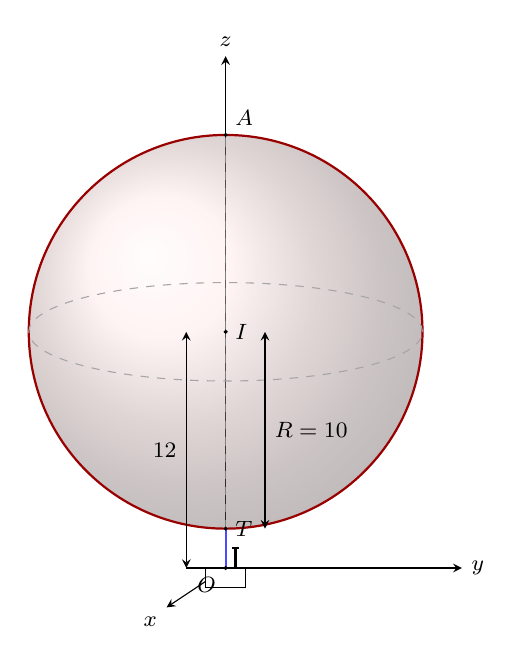
\begin{tikzpicture}[scale=0.25, >=stealth, font=\footnotesize]
					% Trục tọa độ
					\draw[->] (0,0) -- (0,26) node[above]{$z$};
					\draw[->] (-2,0) -- (12,0) node[right]{$y$};
					\draw[->] (0,0) -- (-3,-2) node[below left]{$x$};
					
					% Quả bóng
					\shade[ball color=red!15, opacity=0.4] (0,12) circle (10);
					\draw[thick, red!60!black] (0,12) circle (10);
					\draw[dashed, gray!70] (0,12) ellipse (10 and 2.5);
					
					% Dây và trục
					\draw[thick, blue!70] (0,0) -- (0,2);
					\draw[dashed, gray] (0,2) -- (0,22);
					
					% Hộp thiết bị
					\filldraw[fill=white, draw=black] (-1,-1) rectangle (1,0);
					\draw[thick] (0.5,0) -- (0.5,1) (0.3,1) -- (0.7,1);
					
					% Nhãn
					\filldraw (0,0) circle (2pt) node[below left]{$O$};
					\filldraw (0,12) circle (2pt) node[right]{$I$};
					\filldraw (0,2) circle (2pt) node[right]{$T$};
					\filldraw (0,22) circle (2pt) node[above right]{$A$};
					\draw[<->] (-2,0) -- (-2,12) node[midway, left]{$12$};
					\draw[<->] (2,2) -- (2,12) node[midway, right]{$R=10$};
				\end{tikzpicture}
				\par\textit{Hình 1: Trạng thái đứng yên}
			\end{minipage}
			\quad
			% === HÌNH 2: Trạng thái lệch gió ===
			\begin{minipage}[t]{0.45\linewidth}
				\centering
				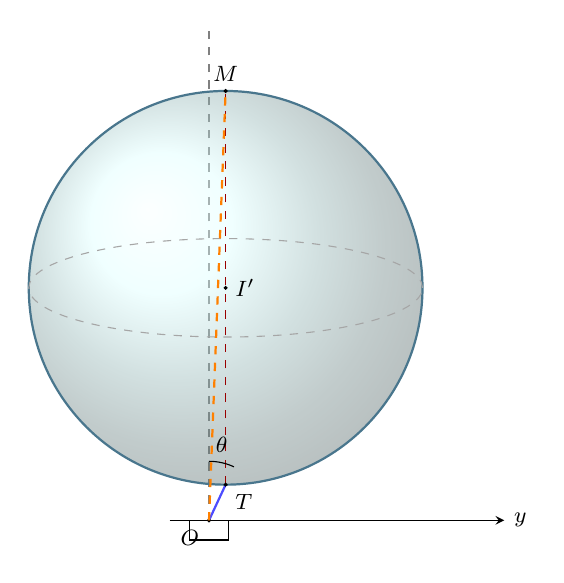
\begin{tikzpicture}[scale=0.25, >=stealth, font=\footnotesize]
					% Trục tham chiếu
					\draw[dashed, gray] (0,0) -- (0,25);
					\draw[->] (-2,0) -- (15,0) node[right]{$y$};
					
					% Góc lệch
					\def\ang{25}
					\coordinate (O) at (0,0);
					\coordinate (T) at ({\ang+90}:2); % Tọa độ cực
					\coordinate (T_pos) at ({2*sin(\ang)}, {2*cos(\ang)});
					\coordinate (I_pos) at ({2*sin(\ang)}, {2*cos(\ang)+10});
					\coordinate (M_pos) at ({2*sin(\ang)}, {2*cos(\ang)+20});
					
					% Quả bóng (giữ phương thẳng đứng)
					\shade[ball color=cyan!20, opacity=0.4] (I_pos) circle (10);
					\draw[thick, cyan!50!black] (I_pos) circle (10);
					\draw[dashed, gray!70] (I_pos) ellipse (10 and 2.5);
					
					% Dây cáp lệch
					\draw[thick, blue!70] (O) -- (T_pos);
					% Trục bóng
					\draw[dashed, red!60!black] (T_pos) -- (M_pos);
					
					% Góc
					\draw (0,3) arc (90:{90-\ang}:3) node[midway, above]{$\theta$};
					
					% Hộp thiết bị
					\filldraw[fill=white, draw=black] (-1,-1) rectangle (1,0);
					
					% Nhãn
					\filldraw (O) circle (2pt) node[below left]{$O$};
					\filldraw (T_pos) circle (2pt) node[below right]{$T$};
					\filldraw (I_pos) circle (2pt) node[right]{$I'$};
					\filldraw (M_pos) circle (2pt) node[above]{$M$};
					
					% Đường nối OM
					\draw[orange, thick, dashed] (O) -- (M_pos);
				\end{tikzpicture}
				\par\textit{Hình 2: Khi có gió thổi lệch $\theta$}
			\end{minipage}
		\end{center}
		
		\textbf{Phân tích chung:}
		Mặt cầu $(S)$ có tâm $I(0; 0; 12)$ và bán kính $R = 10$\,m. Tại gốc $O(0;0;0)$ đặt buồng hành khách.
		Điểm nối dây cáp với đáy quả bóng là $T$. Khi không có gió, quả bóng đứng thẳng nên $T$ nằm trên trục $Oz$ và có cao độ $z_T = z_I - R = 12 - 10 = 2$\,m. Do đó, chiều dài dây cáp $OT = 2$\,m. 
		
		\begin{itemchoice}
			\itemch \textbf{Đúng.} Khoảng cách từ tâm bóng $I(0;0;12)$ đến trạm $O(0;0;0)$ là $OI = \sqrt{0^2+0^2+12^2} = 12$\,m.
			\itemch \textbf{Đúng.} Chiều dài lớn nhất của tổ hợp (từ đáy buồng khách đến đỉnh bóng) là $L = OT + 2R = 2 + 2 \cdot 10 = 22$\,m.
			\itemch \textbf{Sai.} Khi dây cáp lệch $15^\circ$, do phần chứa khí không nghiêng nên véc-tơ $\overrightarrow{TI'}$ (nối từ đáy đến tâm bóng) luôn thẳng đứng hướng lên, $|\overrightarrow{TI'}| = R = 10$.
			\textit{Tính tọa độ:} $\overrightarrow{OT} = (2\sin 15^\circ; 0; 2\cos 15^\circ) \approx (0,5; 0; 1,9)$.
			Vị trí tâm bóng mới: $\overrightarrow{OI'} = \overrightarrow{OT} + \overrightarrow{TI'} = (2\sin 15^\circ; 0; 2\cos 15^\circ + 10)$.
			Độ cao (cao độ $z$) của tâm bóng là $z_{I'} = 2\cos 15^\circ + 10 \approx 11{,}9$\,m $\neq 11{,}2$\,m. 
			\itemch \textbf{Sai.} Khi dây lệch $25^\circ$, điểm xa nhất trên khí cầu là đỉnh $M$.
			Ta có véc-tơ $\overrightarrow{TM}$ thẳng đứng hướng lên và $|\overrightarrow{TM}| = 2R = 20$\,m.
			Sử dụng định lý Cô-sin trong tam giác $OTM$ với góc $\widehat{OTM} = 180^\circ - 25^\circ = 155^\circ$:
			$OM = \sqrt{OT^2 + TM^2 - 2\cdot OT \cdot TM \cdot \cos 155^\circ} = \sqrt{2^2 + 20^2 - 2\cdot 2 \cdot 20 \cdot \cos 155^\circ} \approx 21{,}8$\,m.
			Kết quả $21{,}8$\,m $\neq 18{,}3$\,m. 
		\end{itemchoice}
	}
\end{ex}
%%%=============================%%%

%%%=============EX_16=============%%%
\begin{ex}%[2D6C2-4]%[TDMZZ01]%[Vũ Hồng Toàn]
	Công ty X có giao cho hai xí nghiệp I và II sản xuất một loại sản phẩm Y. Xí nghiệp I sản xuất $60\%$ tổng sản phẩm và có tỉ lệ phế phẩm là $4\%$, xí nghiệp II có tỉ lệ phế phẩm là $2\%$. Để giảm xác suất chọn được phế phẩm, người ta dùng một con xúc xắc cân đối đồng chất để gieo ngẫu nhiên, nếu số chấm thu được không vượt quá $2$ thì chọn một sản phẩm của xí nghiệp I, nếu số chấm lớn hơn $2$ thì chọn ngẫu nhiên một sản phẩm của công ty (tức là của cả hai xí nghiệp). Gọi $A$ là biến cố chọn được phế phẩm, $B$ là biến cố chọn được sản phẩm của xí nghiệp I.
	\choiceTF
	{\True $\mathrm{P}(A\mid B) = 0{,}04$}
	{$\mathrm{P}(B) = 0{,}6$}
	{$\mathrm{P}(A) = 0{,}032$}
	{\True $\mathrm{P}(B\mid A) = \dfrac{11}{13}$}
	\loigiai{
		Gọi $D_1$ là biến cố số chấm thu được của xúc xắc không vượt quá $2$. Ta có $\mathrm{P}(D_1) = \dfrac{2}{6} = \dfrac{1}{3}$.\\
		$D_2$ là biến cố số chấm thu được của xúc xắc lớn hơn $2$. Ta có $\mathrm{P}(D_2) = \dfrac{4}{6} = \dfrac{2}{3}$.\\
		Tỉ lệ sản phẩm của Xí nghiệp I trong công ty $\mathrm{P}(X_1) = 0{,}6$.\\
		Tỉ lệ phế phẩm là $\mathrm{P}(A\mid X_1) = 0{,}04$; $\mathrm{P}(A\mid X_2) = 0{,}02$.\\
		Sơ đồ cây xác suất chọn sản phẩm và kiểm tra phế phẩm
		\begin{center}
			\begin{tikzpicture}[declare function={dai=3.0;cao=0.7;}, >=stealth, font=\footnotesize]
				\tikzset{nhan/.style={minimum size=20pt, font=\small, inner sep=0pt, align=center}}
				\path (0,0) node[nhan] (G) {\textbf{Gốc}};
				\path (dai, 3*cao) node[nhan] (D1) {$D_1$};
				\path (dai, -2*cao) node[nhan] (D2) {$D_2$};
				\path (2*dai, 3*cao) node[nhan] (B1) {$B$};
				\path (2*dai, -cao) node[nhan] (B2) {$B$};
				\path (2*dai, -3*cao) node[nhan] (nB) {$\overline{B}$};
				\path (3*dai, 4*cao) node[nhan] (A1) {$A$};
				\path (3*dai, 2*cao) node[nhan] (nA1) {$\overline{A}$};
				\path (3*dai, 0*cao) node[nhan] (A2) {$A$};
				\path (3*dai, -2*cao) node[nhan] (nA2) {$\overline{A}$};
				\path (3*dai, -2.5*cao-0.4) node[nhan] (A3) {$A$};
				\path (3*dai, -4*cao-0.4) node[nhan] (nA3) {$\overline{A}$};
				
				\draw[->] (G.east) -- (D1.west) node[sloped, pos=0.5, above] {$\dfrac{1}{3}$};
				\draw[->] (G.east) -- (D2.west) node[sloped, pos=0.5, below] {$\dfrac{2}{3}$};
				\draw[->] (D1.east) -- (B1.west) node[sloped, pos=0.5, above] {$1$};
				\draw[->] (D2.east) -- (B2.west) node[sloped, pos=0.5, above] {$0{,}6$};
				\draw[->] (D2.east) -- (nB.west) node[sloped, pos=0.5, below] {$0{,}4$};
				\draw[->] (B1.east) -- (A1.west) node[sloped, pos=0.5, above] {$0{,}04$};
				\draw[->] (B1.east) -- (nA1.west) node[sloped, pos=0.5, below] {$0{,}96$};
				\draw[->] (B2.east) -- (A2.west) node[sloped, pos=0.5, above] {$0{,}04$};
				\draw[->] (B2.east) -- (nA2.west) node[sloped, pos=0.5, below] {$0{,}96$};
				\draw[->] (nB.east) -- (A3.west) node[sloped, pos=0.5, above] {$0{,}02$};
				\draw[->] (nB.east) -- (nA3.west) node[sloped, pos=0.5, below] {$0{,}98$};
			\end{tikzpicture}
		\end{center}
		\begin{itemchoice}
			\itemch Vì sản phẩm thuộc xí nghiệp I thì tỉ lệ phế phẩm luôn là $4\%$ (không phụ thuộc việc gieo xúc xắc). Do đó $\mathrm{P}(A\mid B) = 0{,}04$.
			\itemch Xác suất chọn được sản phẩm Xí nghiệp I là
			\[\mathrm{P}(B) = \mathrm{P}(D_1) \cdot 1 + \mathrm{P}(D_2) \cdot 0{,}6 = \dfrac{1}{3} \cdot 1 + \dfrac{2}{3} \cdot 0{,}6 = \dfrac{11}{15} \approx 0{,}73.\]
			\itemch Xác suất chọn được phế phẩm là
			\[\mathrm{P}(A) = \dfrac{1}{3} \cdot 1 \cdot 0{,}04 + \dfrac{2}{3} \cdot 0{,}6 \cdot 0{,}04 + \dfrac{2}{3} \cdot 0{,}4 \cdot 0{,}02 = \dfrac{13}{375} \approx 0{,}035.\]
			\itemch Xác suất chọn được sản phẩm Xí nghiệp I là phế phẩm
			\[\mathrm{P}(A \cap B) = \dfrac{1}{3} \cdot 1 \cdot 0{,}04 + \dfrac{2}{3} \cdot 0{,}6 \cdot 0{,}04 = \dfrac{11}{375}.\]
			Áp dụng công thức Bayes
			\[\mathrm{P}(B \mid A) = \dfrac{\mathrm{P}(A \cap B)}{\mathrm{P}(A)} = \dfrac{11}{375}\cdot\dfrac{375}{13} = \dfrac{11}{13}.\]
		\end{itemchoice}
	}
\end{ex}
%%%=============================%%%


\Closesolutionfile{ans}

\caukq
\Opensolutionfile{ans}[ans/ansTN-DienKhuyet]

%%%=============EX_17=============%%%
\begin{ex}%[1H8C5-4]%[TDMZZ01]%[Võ Hiệp]
	\immini[thm]{Cho hình lăng trụ đều $ABC. A'B'C'$ có $AA'=8$, $AB=6$. Gọi $M$ là trung điểm của cạnh $CC'$. Hãy tính khoảng cách giữa hai đường thẳng $AB'$ và $A'M$ \textit{(làm tròn kết quả đến hàng phần trăm)}.
	}{
		
		\begin{tikzpicture}[scale=0.7, font=\footnotesize, line join=round, line cap=round, >=stealth]
			\def\a{4}
			\def\h{4}
			\path 	(0:0) coordinate (A)
			++(0:\a) coordinate (C)
			++(-150:3*\a/4) coordinate (B)
			($(A)+(90:\h)$) coordinate (A')
			($(B)+(90:\h)$) coordinate (B')
			($(C)+(90:\h)$) coordinate (C')
			($(C)!.5!(C')$)coordinate (M);
			\draw[dashed] 	(A)--(C) (A')--(M);
			\draw (C)--(C') 	(B)--(B')	(A)--(A') (A)--(B)--(C) (A')--(B')--(C')--cycle
			(A)--(B');
			\foreach \x/\g in {A/180,B/-45,C/0,A'/180,B'/-45,C'/0, M/0}
			\fill[black] 	(\x) circle (1pt)
			($(\g:4mm)+(\x)$) node {$\x$};	
		\end{tikzpicture}
		
	}
	\par
	\shortans[0]{3,53}
	\loigiai{
		\immini{
			Gọi $D$ là điểm sao cho $ABDC$ là hình thoi, $D'$ là điểm thỏa mãn $ABDC. A'B'D'C'$ là hình lăng trụ đứng, $M'$ là trung điểm $DD'$ (như hình vẽ bên).\\
			Khi đó, ta có
			$A'M\parallel B'M' \subset (AB'M')$.\\
			Suy ra $A'M\parallel (AB'M')$.\\
			Do đó $\mathrm{d}(A'M,AB')=\mathrm{d}(A'M,(AB'M'))=\mathrm{d}(A',(AB'M'))$.\\
			Xét hình chóp $M'. AA'B'$.\\
			Vì $ABDC. A'B'D'C'$ là lăng trụ đứng.\\
		}{
			\begin{tikzpicture}[scale=0.7, font=\footnotesize, line join=round, line cap=round, >=stealth]
				\def\a{4}
				\def\h{4}
				\path 	(0:0) coordinate (A)
				++(0:\a) coordinate (C)
				++(-150:3*\a/4) coordinate (B)
				($(B)+(C)-(A)$) coordinate (D)
				($(A)+(90:\h)$) coordinate (A')
				($(B)+(90:\h)$) coordinate (B')
				($(C)+(90:\h)$) coordinate (C')
				($(D)+(90:\h)$) coordinate (D')
				($(C)!.5!(C')$)coordinate (M)
				($(D)!.5!(D')$)coordinate (M')
				;
				\draw[dashed] 	(A)--(C)--(D) (A')--(M) (C)--(C') (B)--(C) (A)--(M')--(M) (A)--(D);
				\draw (A')--(B')--(D')--(C')--cycle (A)--(B)--(D) 	(A)--(B')--(M')
				(A)--(A') (B)--(B') (D)--(D') (B')--(C');
				\foreach \x/\g in {A/180,B/-45,C/0,A'/180,B'/180,C'/0, M/20,M'/20,D/-60,D'/30}
				\fill[black] 	(\x) circle (1pt)
				($(\g:4mm)+(\x)$) node {$\x$};	
			\end{tikzpicture}
		}
		\noindent
		Suy ra $\mathrm{d}(M',(AA'B'))=\mathrm{d}(C,(AA'B'))=\mathrm{d}(C,AB)=6\cdot\dfrac{\sqrt{3}}{2}=3\sqrt{3}$ (đường cao của $\triangle ABC$ đều).\\
		Diện tích tam giác $AB'A'$ là $S_{\triangle AB'A'}=\dfrac{1}{2}\cdot AA'\cdot A'B'=\dfrac{1}{2}\cdot 8\cdot 6 =24$.\\
		Suy ra thể tích $V_{M'. AA'B'}=\dfrac{1}{3}\cdot S_{\triangle AB'A'}\cdot \mathrm{d}(M',(AA'B'))= \dfrac{1}{3}\cdot 24\cdot 3\sqrt{3}=24\sqrt{3}$.\\
		Xét hình chóp $A'. AB'M'$.\\
		Từ giả thiết bài toán và cách dựng hình lăng trụ, ta có các tam giác $\triangle AB'A'$, $\triangle B'D'M'$, $\triangle ADM'$ vuông, $AD=6\sqrt{3}$. Suy ra\\
		$AB'=\sqrt{AA'^2+A'B'^2}=\sqrt{8^2+6^2}=10$.\\
		$B'M'=\sqrt{B'D'^2+D'M'^2}=\sqrt{6^2+4^2}=2\sqrt{13}$.\\
		$AM'=\sqrt{AD^2+DM'^2}=\sqrt{\left(6\sqrt{3}\right)^2+4^2}=2\sqrt{31}$.\\
		Suy ra $S_{\triangle AB'M'}=\sqrt{p(p-AB')(p-B'M')(p-AM')}=3\sqrt{139}$ với $p=\dfrac{AB'+B'M'+AM'}{2}$.\\
		Thể tích $V_{A'. AB'M'}=\dfrac{1}{3}\cdot S_{\triangle AB'M'}\cdot \mathrm{d}(A',(AB'M'))\Rightarrow \mathrm{d}(A',(AB'M'))=\dfrac{3V_{A'. AB'M'}}{S_{\triangle AB'M'}}$.\\
		Mà $V_{A'. AB'M'}= V_{M'. AA'B'}=24\sqrt{3} \Rightarrow \mathrm{d}(A',(AB'M'))=\dfrac{3\cdot24\sqrt{3}}{3\sqrt{139}}\approx 3{,}53$.
	}
\end{ex}
%%%=============================%%%

%%%=============EX_18=============%%%
\begin{ex}%[2D4V3-1]%[TDMZZ01]%[Lương Pho]
	\immini[thm]{Diện tích phần hình phẳng $(H)$ được tô màu vàng trong hình vẽ bên dưới bằng bao nhiêu (\textit{làm tròn kết quả đến hàng phần mười})?}{
		\begin{tikzpicture}[line cap=round,line join=round,>=stealth,xscale=.7,yscale=.5,font=\footnotesize,declare function={
				xmin=-0.5;xmax=7;
				ymin=-0.5;ymax=13;
				b=9-3*sqrt(3);a=-12/(b^2);
				f(\x)=a*(\x-b)^2+12;
			}]
			\fill[pattern=north east lines, pattern color=yellow]
			(0,0)--plot[domain=0:6] (\x, {f(\x)})--(6,8)--cycle;
			\fill[teal!30] (0,0)--(6,0)--(6,8)--cycle;
			\draw (0,0) rectangle (6,12) (0,0)--(6,8);
			\draw[smooth,samples=300] plot[domain=0:6] (\x, {f(\x)});
			\draw[|<->|] (-0.5,0)--(-0.5,12) node[left, pos=0.5]{$12$};
			\draw[|<->|] (0,-0.5)--(6,-0.5) node[below, pos=0.5]{$6$};
			\draw[|<->|] (6.5,8)--(6.5,12) node[right, pos=0.5]{$4$};
			\node at (3,7) {$(H)$};
		\end{tikzpicture}
	}
	\par
	\shortans[0]{29,9}
	\loigiai{
		\immini{Chọn hệ trục tọa độ $Oxy$ như hình vẽ bên.\\
			Xét parabol $(H)\colon y=a(x-x_0)^2+12$ (với $a<0$ và $0<x_0<6$) có đỉnh $I(x_0;12)$.\\
			Điểm $O(0;0)\in (H)$ nên $ax_0^2+12=0\Rightarrow a=-\dfrac{12}{x_0^2}$.\\
			Điểm $A(6;8)\in (H)$ nên
			\begin{eqnarray*}
				&&a(6-x_0)^2+12=8\\
				&\Leftrightarrow&-\dfrac{12}{x_0^2}\left(36-12x_0+x_0^2\right)+12=8\\
				&\Leftrightarrow&8x_0^2-144x_0+432=0\\
				&\Leftrightarrow&\hoac{&x_0=9+3\sqrt{3}>6 &&\text{ (loại)}\\&x_0=9-3\sqrt{3}&&\text{ (nhận).}}
			\end{eqnarray*}
		}{
			\begin{tikzpicture}[line cap=round,line join=round,>=stealth,xscale=.7,yscale=.5,font=\footnotesize,declare function={
					xmin=-1;xmax=7;
					ymin=-1;ymax=13;
					b=9-3*sqrt(3);a=-12/(b^2);
					f(\x)=a*(\x-b)^2+12;
				}]
				\fill[pattern=north east lines, pattern color=yellow]
				(0,0)--plot[domain=0:6] (\x, {f(\x)})--(6,8)--cycle;
				\draw[->] (xmin,0)--(xmax,0) node[shift={(-100:7pt)}]{$x$};
				\draw[->] (0,ymin)--(0,ymax) node[shift={(0:7pt)}]{$y$};
				\fill (0,0) node[shift={(225:9pt)}]{$O$};
				\clip (xmin,ymin) rectangle (xmax,ymax);
				\draw (0,0) rectangle (6,12) (0,0)--(6,8);
				\draw[smooth,samples=300] plot[domain=0:6] (\x, {f(\x)});
				\foreach \x in {6}{
					\fill (\x,0) circle (1pt) node[shift={(-90:7pt)}]{$\x$};}
				\foreach \y/\g in {12/180,8/180}{
					\fill (0,\y) circle (1pt) node[shift={(\g:9pt)}]{$\y$};}
				\foreach \x/\y/\nhan/\g in {6/8/A/0} {
					\draw[dashed] (\x,0) |- (0,\y);
					\fill (\x,\y) circle (1pt) node[shift={(\g:7pt)}]{$\nhan$};
				}
			\end{tikzpicture}
		}
		Với $x_0=9-3\sqrt{3}\Rightarrow a=-\dfrac{2}{9}\left(2+\sqrt{3}\right)$.\\
		Suy ra $(H)\colon y=-\dfrac{2}{9}\left(2+\sqrt{3}\right)\left(x-9+3\sqrt{3}\right)^2+12$.\\
		Diện tích phần màu vàng là
		\[\displaystyle\int\limits_0^6 \Bigg[-\dfrac{2}{9}\left(2+\sqrt{3}\right)\left(x-9+3\sqrt{3}\right)^2+12\Bigg]\mathrm{d}x-\dfrac{1}{2}\cdot 6\cdot 8\approx 29{,}9.\]
	}
\end{ex}
%%%=============================%%%

%%%=============EX_19=============%%%
\begin{ex}%[2H2V2-6]%[TDMZZ01]%[Hà Văn Hảo]
	\immini[thm]{Trong không gian $Oxyz$, coi Trái Đất là một hình cầu có tâm là gốc tọa độ và có bán kính bằng $16$, đơn vị dài trên mỗi trục tọa độ là $400$ km, đường xích đạo nằm trong mặt phẳng $(Oxy)$. Tại điểm $A(0;16;0)$, người ta phóng một tàu vũ trụ (coi như bay thẳng) lên không trung theo hướng của vectơ $\overrightarrow{u} = (2;0;1)$ với tốc độ $10$ km/s. Sau khoảng thời gian $3$ phút thì tàu vũ trụ ở vị trí $B$. Gọi $M$ là điểm nằm trên đường xích đạo và gần với $B$ nhất. Hãy xác định theo kilômét độ dài $MB$ (\textit{làm tròn kết quả đến hàng đơn vị}).}{
		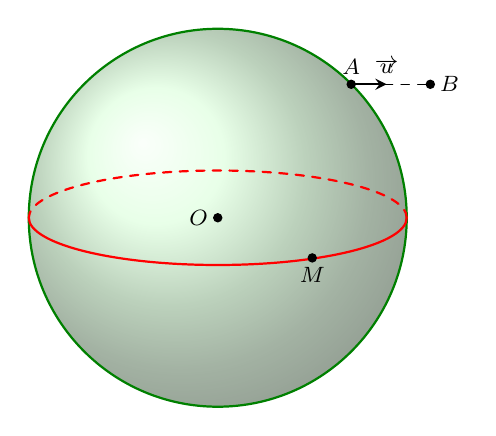
\begin{tikzpicture}[scale=0.15, font=\footnotesize, line join=round, line cap=round, >=stealth]
			\shade[ball color=green!20, opacity=0.6] (0,0) circle (16);
			\draw[thick, color=green!50!black] (0,0) circle (16);
			
			\draw[thick, color=red] (16,0) arc (0:-180:16 and 4);
			\draw[thick, dashed, color=red] (16,0) arc (0:180:16 and 4);
			
			\coordinate (O) at (0,0);
			\coordinate (A) at (11.3, 11.3);
			\coordinate (B) at (18, 11.3);
			\coordinate (M) at (8, -3.4);
			
			\fill (O) circle (0.4) node[left] {$O$};
			\fill (A) circle (0.4) node[above] {$A$};
			\fill (B) circle (0.4) node[right] {$B$};
			\fill (M) circle (0.4) node[below] {$M$};
			
			\draw[->, thick] (A) -- ++(3,0) node[above] {$\overrightarrow{u}$};
			\draw[dashed] (A) -- (B);
		\end{tikzpicture}
	}
	\par 
	\shortans[0]{829}
	\loigiai{
		\begin{itemize}
			\item Xác định tọa độ điểm $B$\\
			Đổi thời gian $t = 3$ phút $= 180$ giây.\\
			Quãng đường tàu bay được theo đơn vị km $s = v \cdot t = 10 \cdot 180 = 1\,800$ km.\\
			Đổi quãng đường sang đơn vị tọa độ $d = \dfrac{1\,800}{400} = 4{,}5$.\\
			Vectơ chỉ phương của quỹ đạo là $\overrightarrow{u} = (2; 0; 1)$, có độ dài $|\overrightarrow{u}| = \sqrt{2^2 + 0^2 + 1^2} = \sqrt{5}$.\\
			Tọa độ điểm $B$ được xác định bởi
			\[ \overrightarrow{AB} = \dfrac{d}{\left|\overrightarrow{u}\right|} \cdot \overrightarrow{u} = \dfrac{4{,}5}{\sqrt{5}} \cdot (2; 0; 1) = \left( \dfrac{9}{\sqrt{5}}; 0; \dfrac{4{,}5}{\sqrt{5}} \right). \]
			Vì $A(0; 16; 0)$, tọa độ điểm $B$ là
			\[ B = \left( \dfrac{9}{\sqrt{5}}; 16; \dfrac{4{,}5}{\sqrt{5}} \right) \approx (4{,}025; 16; 2{,}012). \]
			\item Xác định tọa độ điểm $M$\\
			Đường xích đạo nằm trong mặt phẳng $(Oxy)$ và là đường tròn tâm $O$, bán kính $R = 16$. Phương trình đường xích đạo $\heva{&x^2 + y^2 = 16^2 \\ &z = 0.}$\\
			Gọi $B'$ là hình chiếu của $B$ lên mặt phẳng $(Oxy)$, ta có $B' \left( \dfrac{9}{\sqrt{5}}; 16; 0 \right)$.\\
			Điểm $M$ trên đường xích đạo gần $B$ nhất chính là giao điểm của tia $OB'$ với đường tròn xích đạo.\\
			Độ dài $OB' = \sqrt{\left( \dfrac{9}{\sqrt{5}} \right)^2 + 16^2} = \sqrt{\dfrac{81}{5} + 256} = \sqrt{272{,}2} \approx 16{,}5$.\\
			Tọa độ điểm $M$ thỏa mãn $\overrightarrow{OM} = \dfrac{R}{OB'} \cdot \overrightarrow{OB'}$, do đó
			\[ \overrightarrow{OM} = \dfrac{16}{OB'} \cdot \overrightarrow{OB'} = \left( \dfrac{16 \cdot \dfrac{9}{\sqrt{5}}}{OB'}; \dfrac{16 \cdot 16}{OB'}; 0 \right). \]
			\item Tính độ dài $MB$\\
			Khoảng cách $MB$ trong không gian được tính bởi
			\[ MB^2 = (B_x - M_x)^2 + (B_y - M_y)^2 + (B_z - M_z)^2.\]
			Nhận thấy $(B_x - M_x)^2 + (B_y - M_y)^2$ là bình phương khoảng cách từ $B'$ đến $M$ trên mặt phẳng $(Oxy)$, tức là $(OB' - R)^2$.
			\[ MB = \sqrt{(OB' - R)^2 + B_z^2} .\]
			Thay các giá trị vào
			\[ MB = \sqrt{(\sqrt{272{,}2} - 16)^2 + \left( \dfrac{4{,}5}{\sqrt{5}} \right)^2} \approx \sqrt{(16{,}4985 - 16)^2 + 2{,}025} \approx \sqrt{0{,}2485 + 4{,}05} \approx 2{,}0733.\]
			Đổi sang đơn vị km $MB = 2{,}0733 \cdot 400 \approx 829{,}32$ km.\\
			Làm tròn đến hàng đơn vị, ta được $829$ km.
		\end{itemize}
	}
\end{ex}
%%%=============================%%%

%%%=============EX_20=============%%%
\begin{ex}%[0D0C2-5]%[TDMZZ01]%[Lê Hồ Quang Minh]
	\immini[thm]{Cho hình đa giác đều $(H)$ gồm có $4\,320$ đỉnh. Gọi $A$ là tập chứa tất cả các đa giác đều có các đỉnh là đỉnh của $(H)$. Chọn ngẫu nhiên từ $A$ ra một đa giác. Gọi $\mathrm{P}$ là xác suất để chọn được đa giác có góc ở đỉnh bằng $150^\circ$. Hãy tính $1\,000\mathrm{P}$ \textit{(làm tròn kết quả đến hàng đơn vị)}.}{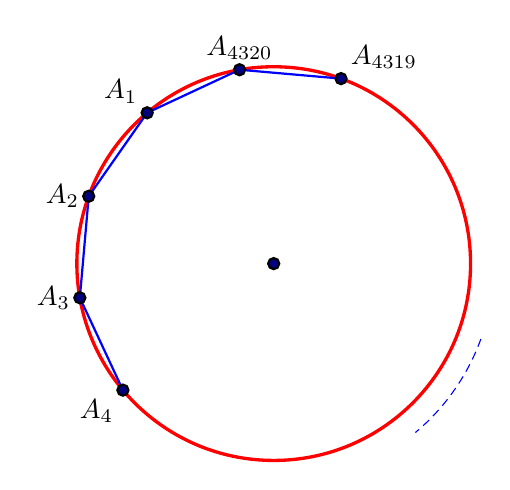
\begin{tikzpicture}
			\def\R{2.5}
			\def\n{4320}
			\draw[red, very thick] (0,0) circle (\R);
			\filldraw[fill=blue!50!black, thick] (0,0) circle (2pt);
			\coordinate (A4320) at (100:\R);
			\coordinate (A1) at (130:\R);
			\coordinate (A2) at (160:\R);
			\coordinate (A3) at (190:\R);
			\coordinate (A4) at (220:\R);
			\coordinate (A4319) at (70:\R);
			\draw[blue, thick] (A4319) -- (A4320) -- (A1) -- (A2) -- (A3) -- (A4);
			\foreach \p in {A4319, A4320, A1, A2, A3, A4} {
				\filldraw[fill=blue!50!black, thick] (\p) circle (2pt);
			}
			\node[above right] at (A4319) {$A_{4319}$};
			\node[above] at (A4320) {$A_{4320}$};
			\node[above left] at (A1) {$A_1$};
			\node[left] at (A2) {$A_2$};
			\node[left] at (A3) {$A_3$};
			\node[below left] at (A4) {$A_4$};
			\draw[blue, dashed, dash pattern=on 3pt off 2pt] 
			(-20:\R+0.3) arc (-20:-50:\R+0.3);
	\end{tikzpicture}}
	\par 
	\shortans[oly]{42}
	\loigiai{
		Giả sử đa giác đều cần tìm có $n$ cạnh ($n \ge 3$). Số đo góc ở đỉnh của đa giác đều $n$ cạnh là
		$$\alpha = \dfrac{(n-2) \cdot 180^\circ}{n} = 150^\circ \Rightarrow n = 12.$$
		Các đa giác đều có đỉnh là đỉnh của $(H)$ phải có số cạnh $n$ là ước của $4\,320$ và $n \ge 3$.\\
		Số lượng đa giác đều ứng với mỗi ước $n$ là $\dfrac{4\,320}{n}$.\\
		Số đa giác đều $12$ cạnh có đỉnh là đỉnh của $(H)$ là $ \dfrac{4\,320}{12} = 360$ (đa giác).\\
		Ta có $4\,320 = 2^5 \cdot 3^3 \cdot 5^1$.\\
		Tổng các ước của $4\,320$ là
		$\dfrac{2^6-1}{2-1} \cdot \dfrac{3^4-1}{3-1} \cdot \dfrac{5^2-1}{5-1} = 63 \cdot 40 \cdot 6 = 15\,120$.\\
		Tổng số đa giác đều trong tập $A$ là
		$$n(A) = \sum\limits_{n|4\,320, n \ge 3} \dfrac{4\,320}{n} = \left( \sum\limits_{d|4\,320} d \right) - \dfrac{4\,320}{1} - \dfrac{4\,320}{2} = 15\,120 - 4\,320 - 2\,160 = 8\,640.$$
		Xác suất chọn được đa giác có góc $150^\circ$ là
		$\mathrm{P} = \dfrac{360}{8\,640} = \dfrac{1}{24}$.\\
		Vậy $1\,000\cdot \mathrm{P} = \dfrac{1\,000}{24} \approx 42$.
	}
\end{ex}
%%%=============================%%%

%%%=============EX_21=============%%%
\begin{ex}%[0H9V1-6]%[TDMZZ01]%[Nguyễn Đức Tuấn Anh]
	\immini[thm]{Trên mặt phẳng toạ độ với đơn vị dài trên mỗi trục là kilômét có một khẩu pháo đặt tại gốc toạ độ và một mục tiêu chuyển động thẳng đều ở thời điểm ban đầu có toạ độ $A(0{,}5; 6)$. Ở thời điểm $20$ giây khoảng cách từ mục tiêu đến $3$ radar đặt tại $O$, $G(0{,}1; 0)$, $H(0; 0{,}1)$ lần lượt là $\dfrac{\sqrt{97}}{2}$ km; $\dfrac{\sqrt{2\,386}}{10}$ km; $\dfrac{2\sqrt{146}}{5}$ km. Ngay sau đó từ khẩu pháo bắn ra một viên đạn bay với tốc độ $v_0$ m/s để đón bắt mục tiêu. Hãy tính theo đơn vị m/s giá trị nhỏ nhất $v_0$ (\textit{làm tròn kết quả đến hàng đơn vị}).}{
		\begin{tikzpicture}[scale=1, font=\footnotesize, line join=round, line cap=round, >=stealth]
			\draw[->] (-0.5,0) -- (6,0) node[below] {$x$};
			\draw[->] (0,-0.5) -- (0,5) node[left] {$y$};
			\node at (0,0) [below left] {$O$};
			\path  
			(0,0) coordinate (O)
			(0.5,0) coordinate (G)
			(0,0.5) coordinate (H)
			(0.5,4.5) coordinate (A1)
			(4.5,0.5) coordinate (A2)
			($(A1)!0.1!(A2)$) coordinate (A)
			;
			\draw[rounded corners=10pt, blue, thick,fill=cyan!40] (0.3,0.3) rectangle (6,5);
			\fill (O) circle (1.5pt)
			(G) circle (1.5pt) node[below] {$G$}
			(H) circle (1.5pt) node[left] {$H$}
			(A) circle (1.5pt) node[above right] {$A$};
			\draw[dashed] (A1)--(A2);
			\draw[->, blue, thick] (O) -- (1.5,1) node[pos=.8, above] {$\overrightarrow{v_0}$};
			\node at (4.75, 2.5) {\textbf{Mặt biển}};
			\node at (-0.8,-0.8) {Khẩu pháo};
		\end{tikzpicture}
	}
	\par
	\shortans[0]{99}
	\loigiai{
		Gọi vị trí mục tiêu tại thời điểm $t=20$ s là $B(x; y)$.\\
		Theo giả thiết, khoảng cách từ $B$ đến các radar là
		\begin{itemize}
			\item $OB^2 = x^2 + y^2 = \left(\dfrac{\sqrt{97}}{2}\right)^2 = \dfrac{97}{4} = 24{,}25$. \quad$(1)$
			\item $GB^2 = (x-0{,}1)^2 + y^2 = \left(\dfrac{\sqrt{2386}}{10}\right)^2 = 23{,}86$. \quad $(2)$
			\item $HB^2 = x^2 + (y-0{,}1)^2 = \left(\dfrac{2\sqrt{146}}{5}\right)^2 = 23{,}36$. \quad$(3)$
		\end{itemize}
		Từ $(1)$ và $(2) \Rightarrow x^2 - (x-0{,}1)^2 = 24{,}25 - 23{,}86 = 0{,}39 \Rightarrow 0{,}2x - 0{,}01 = 0{,}39 \Rightarrow x = 2$.\\
		Từ $(1)$ và $(3) \Rightarrow y^2 - (y-0{,}1)^2 = 24{,}25 - 23{,}36 = 0{,}89 \Rightarrow 0{,}2y - 0{,}01 = 0{,}89 \Rightarrow y = 4{,}5$.\\
		Vậy tại $t=20$ s, mục tiêu ở vị trí $B(2; 4{,}5)$.\\
		Vận tốc của mục tiêu là
		\[\overrightarrow{v} = \dfrac{\overrightarrow{AB}}{20} = \dfrac{(2 - 0{,}5; 4{,}5 - 6)}{20}=(0{,}075; -0{,}075) \text{ (km/s)}.\]
		Giả sử đạn bắn ra tại thời điểm $t=20$ s và gặp mục tiêu sau khoảng thời gian $t' > 0$.\\
		Khi đó vị trí gặp nhau là $M(2 + 0{,}075t'; 4{,}5 - 0{,}075t')$.\\
		Quãng đường đạn bay được là $S = v \cdot t' = OM$.
		Khi đó
		\[v^2 = \dfrac{OM^2}{t'^2} = \dfrac{(2 + 0{,}075t')^2 + (4{,}5 - 0{,}075t')^2}{t'^2} = \left(\dfrac{2}{t'} + 0{,}075\right)^2 + \left(\dfrac{4{,}5}{t'} - 0{,}075\right)^2.\]
		Đặt $X = \dfrac{1}{t'} > 0$, ta cần tìm giá trị nhỏ nhất của hàm số
		\[f(X) = (2X + 0{,}075)^2 + (4{,}5X - 0{,}075)^2 = 24{,}25X^2 - 0{,}375X + 0{,}01125.\]
		Đây là tam thức bậc hai có hệ số $a = 24{,}25 > 0$, nên đạt giá trị nhỏ nhất tại $X = \dfrac{0{,}375}{2 \cdot 24{,}25} = \dfrac{3}{388}$.\\
		Giá trị nhỏ nhất là $f_{\min} = 0{,}01125 - \dfrac{0{,}375^2}{4 \cdot 24{,}25}$.\\
		Suy ra $v_{\min} = \sqrt{f_{\min}} \approx 0{,}098996 \text{ km/s} \approx 99 \text{ m/s}.$
	}
\end{ex}
%%%=============================%%%

%%%=============EX_22=============%%%
\begin{ex}%[0D0C2-2]%[TDMZZ01]%[Nguyễn Thành Hậu]
	Hiện tại đã có $6\,000$ em học sinh TDM 2K8 và đang có hơn $20$ giải Nhất tỉnh Toán.
	Tại tỉnh Phú Thọ ở một lớp 12 của một trường THPT có hai bạn Minh Châu và Vi Tiến Hân cùng đăng kí học Toán thầy Ái TDM và cùng đạt Nhất thủ khoa tỉnh Toán.
	Thầy Ái chỉ trao giải thưởng \textbf{THỦ KHOA TOÁN TỈNH} mỗi tỉnh một em cho nên muốn chọn ra một bạn để trao giải bằng cách cho mỗi bạn cầm hai con xúc xắc cân đối đồng chất và cùng gieo, bạn nào có tổng số chấm lớn hơn thì được chọn, bằng điểm thì gieo lại. Hãy tính xác suất để bạn Minh Châu nhận được phần thưởng \textbf{THỦ KHOA TOÁN TỈNH} ngay sau lần gieo đầu tiên (\textit{làm tròn kết quả đến hàng phần trăm}).
	\par
	\shortans[0]{0{,}44}
	\loigiai{Ta sẽ tính xác suất mà hai bạn Châu và Hân có tổng số chấm bằng nhau ở lần gieo đầu tiên.\\
		Tổng số chấm của hai con xúc xắc chỉ có thể là $2$, $3$, $\ldots$, $12$. Giả sử tổng số chấm của hai bạn Châu và Hân đều là $n$ $(2\le n\le 12)$. Gọi $x_{1}$, $x_{2}$, $1\le x_{1}, x_{2}\le 6$ là số chấm xuất hiện khi gieo lần thứ nhất, thứ hai của bạn Châu, khi đó \[x_{1}+x_{2}=n.\]
		\begin{itemize}
			\item \textbf{Trường hợp 1}.\\
			Khi $2\le n\le 7$,
			ta có tất cả $n-1$ cặp $(x_{1},x_{2})$ có thể ($x_{1}$ lần lượt nhận các giá trị từ $1$ đến $n-1$ thì $x_{2}$ lần lượt nhận các giá trị từ $n-1$ đến $1$, và hiển nhiên $1\le x_{1}, x_{2}\le 6$ ).\\
			Vì thế, xác suất để bạn Châu có tổng số chấm bằng $n$ là $\dfrac{n-1}{6\cdot 6}=\dfrac{n-1}{36}$.\\
			Tương tự, xác suất bạn Hân cũng có tổng số chấm bằng $n$ là $\dfrac{n-1}{36}$.\\
			Do đó, xác suất để hai bạn có tổng số chấm cùng bằng $n$ trong trường hợp này là $\left(\dfrac{n-1}{36}\right)^{2}$.
			\item \textbf{Trường hợp 2}.\\
			Với $8\le n\le 12$, ta có tất cả $13-n$ cặp $(x_{1},x_{2})$ có thể ($x_{1}$ lần lượt nhận các giá trị từ $n-6$ đến $6$ thì $x_{2}$ lần lượt nhận các giá trị từ $6$ đến $n-6$, và hiển nhiên $1\le x_{1}, x_{2}\le 6$ ).\\
			Do đó, xác suất để hai bạn có tổng số chấm cùng bằng $n$ trong trường hợp này là $\left(\dfrac{13-n}{36}\right)^{2}$.
		\end{itemize}
		Xác suất để hai bạn có tổng số chấm bằng nhau là \[\displaystyle\sum\limits_{n=2}^{7}\left(\dfrac{n-1}{36}\right)^{2}+\displaystyle\sum\limits_{n=8}^{12}\left(\dfrac{13-n}{36}\right)^{2}=\dfrac{73}{648}.\]
		Ta thấy rằng xác suất để bạn Châu có tổng số chấm lớn hơn bằng xác suất để bạn Hân có tổng số chấm lớn hơn nên xác suất này bằng \[\dfrac{1-\dfrac{73}{648}}{2}=\dfrac{575}{1296}\approx 0{,}44.\]
		Vậy xác suất để bạn Minh Châu nhận được phần thưởng \textbf{THỦ KHOA TOÁN TỈNH} ngay sau lần gieo đầu tiên là $0{,}44$.
	}
\end{ex}
%%%=============================%%%
\Closesolutionfile{ans}
\newpage
\indapan{12}{ans/ansTN-Dung}
\indapan[TF]{2}{ans/ansTN-DungSai}
\indapan[SA]{6}{ans/ansTN-DienKhuyet}
%%%%%%%%%%%%%%
%%nhãn kết thúc đề (để đếm số trang tự động mỗi đề)
\label{B\thedeso}